%
%-------------------------------------------------------------------------------
% ILC TDR Part III - Master file
%-------------------------------------------------------------------------------
%
\documentclass[11pt,twoside]{ILCTDR}
%\usepackage[english]{babel}
%\usepackage{blindtext}


%\usepackage{mytrc_style}

%FG: inserted multirow:
\usepackage{multirow} 
%

\usepackage{savesym}
\savesymbol{iint}
\savesymbol{iiint}
\usepackage{amsmath}
\restoresymbol{}{iint}
\restoresymbol{}{iiint}



%\usepackage{savesym}
%\savesymbol{iint}
%\savesymbol{iiint}
%\usepackage[maybess]{heppennames2} %symbols for physics processes (from CERN) ACHTUNG da ist amsmath dahinter
%\restoresymbol{}{iint}
%\restoresymbol{}{iiint}
% Ties Behnke: added ams math packages for symbols on request from Yasuhiro
%\usepackage{amsmath}
\usepackage{amssymb}
\usepackage{enumitem}
\usepackage{booktabs}

 

%\usepackage{cite}
%
% Directories containing figures
%
\graphicspath{
   {./Introduction/figs/}
   {./Detector/figs/}
   {./figs/}
   {./ILC/figs/}
   {./ILDfigs/}
   {./Integration/figs/}
   {./Modelling/figs/}
   {./Performance/figs/}
   {./References/figs/}
}
%


%\newcommand{\vbdlspacing}{\\[-15pt]}
%\newcommand{\vbabovecaption}{\vspace{-24pt}}
%\newcommand{\vbbelowcaption}{\vspace{-12pt}}
%\newcommand{\vbabove}{\vspace{-12pt}}
%\newcommand{\vbbelow}{\vspace{-12pt}}
%\newcommand{\itemspace}{\vspace{-6pt}}

%\renewcommand{\thepage}{\arabic{chapter}.\arabic{section}-\arabic{page}}
%\renewcommand{\thefigure}{\arabic{chapter}.\arabic{section}-\arabic{figure}}
%\renewcommand{\thetable}{\arabic{chapter}.\arabic{section}-\arabic{table}}

%\newcommand\writer[1]{{\vspace{-2mm}\noindent Edited by #1}\vspace{1mm}}
%\newcommand\writer[1]{{\marginpar{\small \begin{minipage}{2cm}{Author:\\#1}\end{minipage}}}}
%\newcommand\writer[1]{{\small \noindent Authors: #1}}
\newcommand\writer[1]{}

\newcommand\epluseminus{{\mathrm e}^+{\mathrm e}^-}

% from ILD LOI
%end from ILD LOI


\renewcommand\floatpagefraction{.98}
\renewcommand\topfraction{.98}
\renewcommand\bottomfraction{.98}

\setcounter{totalnumber}{4}
\setcounter{topnumber}{4}

%\renewcommand{\topfraction}{0.8}
\renewcommand{\textfraction}{.05}   

\renewcommand{\arraystretch}{1.15}
 
\newcommand{\eplus}{\mathrm{e}^+}
\newcommand{\eminus}{\mathrm{e}^-}
%\newcommand{\epem}{\eplus\eminus}%
\newcommand{\mpmm}{\mu^+\mu^-}
\newcommand{\tptm}{\tau^+\tau^-}
\newcommand{\lplm}{\ell^+\ell^-}
\newcommand{\eeX}{\epem X}
\newcommand{\mmX}{\mpmm X}
\newcommand{\Zzero}{\mathrm{Z}}
\newcommand{\Wboson}{\mathrm{W}}
\newcommand{\WpWm}{\Wboson^+\Wboson^-}
\newcommand{\Higgs}{\mathrm{H}}
\newcommand{\Ptau}{P_\tau}
\newcommand{\qq}{\mathrm{q}\overline{\mathrm{q}}}
\newcommand{\ttbar}{\mathrm{t}\overline{\mathrm{t}}}
\newcommand{\uubar}{\mathrm{u}\overline{\mathrm{u}}}
\newcommand{\ccbar}{\mathrm{c}\overline{\mathrm{c}}}
\newcommand{\bbbar}{\mathrm{b}\overline{\mathrm{b}}}
\newcommand{\ddbar}{\mathrm{d}\overline{\mathrm{d}}}
\newcommand{\ssbar}{\mathrm{s}\overline{\mathrm{s}}}
\newcommand{\nubar}{\overline{\nu}}
\newcommand{\GammaZ}{\Gamma_\Zzero}
\newcommand{\GammaW}{\Gamma_\Wboson}
\newcommand{\mZ}{m_\Zzero}
\newcommand{\mW}{m_\Wboson}
\newcommand{\mH}{m_\Higgs}
\newcommand{\topquark}{\mathrm{t}}
\newcommand{\mtop}{m_\topquark}
\newcommand{\Gtop}{\Gamma_\topquark}
\newcommand{\roots}{\sqrt{s}}
\newcommand{\rmsn}{\mathrm{rms}_{90}}
\newcommand{\rECAL}{R}
\newcommand{\stau}{\mbox{$\tilde{\tau}$}}
\def\XN#1{\mbox{$ \tilde{\chi}^0_#1$}}
\newcommand{\smur}    {\mbox{$ \tilde{\mu}_{\mathrm R}$}}
\newcommand{\smul}    {\mbox{$ \tilde{\mu}_{\mathrm L}$}}
\def\MXN#1{\mbox{$ M_{\tilde{\chi}^0_#1}$}}
\newcommand{\mstone}  {\mbox{$ M_{\tilde{\tau}_1} $}}
\newcommand{\gev}{GeV}
\newcommand{\mum}{\mathrm \mu m}

% temporary fix for DAQ chapter
%\newcommand{\fixme}{FIXME} % command for comments 
%\newcommand{\fixme}[1]{\textbf{FIXME: \textsf{(#1)}}} % command for comments 
\newcommand{\fixme}[1]{} % Temporary remove all comments
% Units spacing and formatting 
%Used in 3_Detector/ild-daq.tex and 2_Subsystems/Calo/HCAL.tex
\newcommand{\unit}[1]{\ensuremath{\mathrm{\,#1}}}
\renewcommand{\u}[1]{\unit{#1}}   
%\newcommand{\us}{\hbox{\textmu}s}
\newcommand{\smH}{\ensuremath{h}\xspace}  % SM higgs 
\newcolumntype{x}[1]{>{\centering\arraybackslash\hspace{0pt}}p{#1}}
\newcommand{\DBDnumbers}{}

\newcommand{\ILDfigure}{\thisfloatsetup{floatwidth=\SfigwFull,capposition=beside} \begin{figure}}
\newcommand{\DBDtable}{\thisfloatsetup{floatwidth=\SfigwFull,capposition=beside}
\begin{table}}

% Chapters to process
%
%\listfiles
%\includeonly{%
% ./ILD-introduction,%
%  ./ILD-summary,%
%}
% Enable an index
%
%%%\makeindex
%
% Enable a list of abbreviations (nomenclature)
%
\makenomenclature
%
%-------------------------------------------------------------------------------
% The document starts here
%-------------------------------------------------------------------------------
%
\begin{document}
%

%\newcommand{\volumetitle}{ILD}
\setcounter{chapter}{0}
\setcounter{part}{1}
%
% Set chapter number
%
\setcounter{chapter}{99}
%
%------------------------------------------------------------------------------
% Frontpage, Introduction, List of Authors, etc. (which have Roman numeral for page numbers)
% start here
%------------------------------------------------------------------------------
%
\frontmatter
%\input{./authors}
%
% Front page
%
%
% Title page
%
\begin{titlepage}
\begin{center}
~
 ~\vskip 4cm

    {\huge  INTERNATIONAL} 
    {\huge  LARGE} 
    {\huge  DETECTOR}
    
  \vskip 1.2cm

    {\huge \bfseries I}
    {\huge \bfseries D}
    {\huge \bfseries R}

  \vskip 1.2cm

%\vskip 3cm

    %{\huge Volume 1:~~~EXECUTIVE SUMMARY}

%\vskip 3cm

{\huge ILD Detector Collaboration} \\
    
  \vskip 0.5cm

{\huge }

  \vskip 3cm

    {\huge Draft Version 5-10-2019}

\end{center}
\end{titlepage}

\newpage\thispagestyle{empty}
\cleardoublepage


%\begin{minipage}{0.95\textwidth}{
%{\Large Editor:} 
\chapter*{ILD Editors}
% \vskip 0.25cm
%\begin{center}
\noindent Main Editors:\\
Ties Behnke, Kiyotomo Kawagoe

\vspace*{2mm}

\noindent Detector layout, technologies and Integration:\\
Karsten Buesser, Claude Vallee

\vspace*{2mm}
\noindent Physics:\\
Keisuke Fujii, Jenny List

\vspace*{2mm}
\noindent Software:\\
Frank Gaede, Akiya Miyamoto

\vspace*{2mm}
\noindent Performance:\\
Keisuke Fujii, Jenny List

\vspace*{2mm}
\noindent Costing:\\
Henri Videau, Karsten Buesser

%\newcommand{\DBDinst}[2]{\noindent  $^{\;\;\:\:#1}$\begin{minipage}[t]{0.95\textwidth}{#2}\end{minipage}\\}
%{
%\footnotesize
%\DBDinst{1}{Cambridge University, Cambridge, UK}
%\DBDinst{2}{CEA Saclay, Paris, France}
%\DBDinst{3}{CERN, Geneva, Switzerland}
%\DBDinst{4}{CIEMAT, Madrid, Spain}
%\DBDInst{5}{DESY, Hamburg and Zeuthen, Germany}
%\DBDinst{6}{IFCA, Cantabria, Spain}
%\DBDinst{7}{IFIC, Valencia, Spain}
%\DBDinst{8}{IN2P3, Lyon, France}
%\DBDinst{9}{IPHC, Strassbourg, Frnace}
%\DBDinst{10}{ITEP. Moscow. Russia}
%\DBDinst{11}{KEK, Tokyo, Japan}
%\DBDinst{12}{LAPCUPDP, Paris, France}
%\DBDinst{13}{LLR, Paris, France}
%\DBDinst{14}{MPI, Munich, Germany}
%\DBDinst{15}{Russian Academy of Science, Russia}
%\DBDinst{16}{Shinshu University, Matsumoto City, Japan}
%\DBDinst{17}{Tel Aviv University, Tel Aviv, Israel}
%\DBDinst{18}{Tohoku University, Sendai, Japan}
%\DBDinst{19}{Tokyo University, Tokyo, Japan}
%\DBDinst{20}{University of Victoria, Canada}
%}
%

%\end{center}



%%
% \vskip 3cm
%%
%\end{flushright}
%}
%\end{minipage}
%
%\newpage\thispagestyle{empty}
%\begin{center}
%~
% ~\vskip 5cm
%\end{center}
%
%\newpage\thispagestyle{empty}
%

%
%------------------------------------------------------------------------------
% Here are the introductory front-matter chapters
%------------------------------------------------------------------------------
%
% List of contributors
%
\cleardoublepage\setcounter{page}{1}
%\chapter*{List of Contributors} 
%\addcontentsline{toc}{chapter}{List of Contributors}
%
% List of Authors
%
%\begin{center}
%\input{./frontmatter/Authors.tex}
%\end{center}
%
% Acknowledgements
%
%\chapter*{Acknowledgements} 
%\addcontentsline{toc}{chapter}{Acknowledgements}
%\input{./frontmatter/Acknowledgements.tex}
%
% Table of contents
%
\tableofcontents 
\addcontentsline{toc}{chapter}{Contents}
%
% Want to set counter for section numbering to 0 for preface (\textit{i.e.}, Executive Summary)
% This means that the sections will not be numbered, but will appear in the TOC and
% on the running headers (odd pages only).
\setcounter{secnumdepth}{0}
%------------------------------------------------------------------------------
% frontmatter ends here
%------------------------------------------------------------------------------
%
%%\setcounter{page}{1}
%\setcounter{figlcl}{0}
%\setcounter{tablcl}{0}
\setcounter{secnumdepth}{3} \setcounter{subsection}{0}
\setcounter{subsubsection}{0}
\usecounter{subsubsection}

%
%------------------------------------------------------------------------------
% Main matter starts here  (it has arabic numerals)
%------------------------------------------------------------------------------
%
\mainmatter
%
% Start from page 1
%
\setcounter{page}{1}
%
% Introduction and Overview
%
\setcounter{chapter}{0}
%\setcounter{page}{1}
%\setcounter{figlcl}{0}
%\setcounter{tablcl}{0}
\setcounter{secnumdepth}{3} \setcounter{subsection}{0}
\setcounter{subsubsection}{0}
\usecounter{subsubsection}


% 18.1.2013 use the performnace and analysis section which include results
\renewcommand{\DBDnumbers}{-numbers}

\chapter{Introduction}
\writer{Ties Behnke, Kiyotomo Kawagoe}{2}
The ILD detector is a proposed detector for the international linear collider, ILC. It has been developed over the last 10 years within a proto-collaboration with the goal to develop and eventually propose a fully integrated detector for the ILC. 

The fundamental ideas and concepts behind the ILD detector have been discussed in two previous documents, the letter of intent \cite{ild:bib:ILDloi} and the detailed baseline document, DBD \cite{ild:bib:ILDDBD}. This document summarises the overall design of the detector, describes developments since the publishing of the DBD, and describes in more detail an effort to optimize the ILD detector. 

The ILD detector concept has been designed as a multi-purpose detector. It should deliver excellent physics performance for collision energies between 90~Gev and 1~TeV, the largest possible energy reach of the ILC. The ILD detector has been optimized to perform excellentLY at the initial ILC energy of 250 GeV. 

The science which will be done at the ILC requires a true multi-purpose detector. A central element of the design has been the capability of the detector to reconstruct precisely complex hadronic final states as well as more events with leptons or missing energy in the final state. Thus traditional precision detector elements as vertex detectors are combined in an overall design philosophy called particle flow, which has been developed for optimal hadronic event reconstruction.

The high precision vertex detector positioned very closely to the interaction point is followed by a hybrid tracking layout, realised as a combination of silicon tracking with a time projection chamber, and a calorimeter system. The complete system is located inside a large solenoid providing a magnetic field of 3.5-4 T. On the outside of the coil, the iron return yoke is instrumented as a muon system and as a tail catcher calorimeter. 

The vertex detector is realised as a multi-layer pixel-vertex detector (VTX), with three super-layers each comprising two layers. The detector has a pure barrel geometry. To minimise the occupancy from background hits,
the first super-layer is only half as long as the outer two. Whilst the underlying detector technology has not yet been decided, 
the VTX is optimised for point resolution and minimum material thickness. 
	
A system of silicon strip and pixel detectors surrounds the VTX detector. In the barrel, two layers of silicon strip detectors (SIT) are arranged to bridge the gap between the VTX and the TPC. In the forward region, a system of two silicon-pixel disks and five silicon-strip disks (FTD) provides low angle tracking coverage.

A distinct feature of ILD is a large volume time projection chamber (TPC) with up to 224 points per track. The TPC is optimised for 3-dimensional point resolution and minimum material in the field cage and in the end-plate. It also allows d$E$/d$x$ based particle identification.

Outside the TPC a system of Si-strip detectors in between the TPC and the ECAL (SET), provide additional high precision space points which improve the tracking performance and provide additional
    redundancy in the regions between the main tracking volume and the calorimeters. 

A highly segmented electromagnetic calorimeter (ECAL) provides up to 30 samples in depth and small transverse cell size, split into a barrel and an end cap system. For the absorber Tungsten has been chosen, for the sensitive area silicon diodes or scintillator strips are considered.
\thisfloatsetup{floatwidth=\SfigwFull,capposition=beside}
\begin{figure}[t!]
\begin{tabular}{cc}
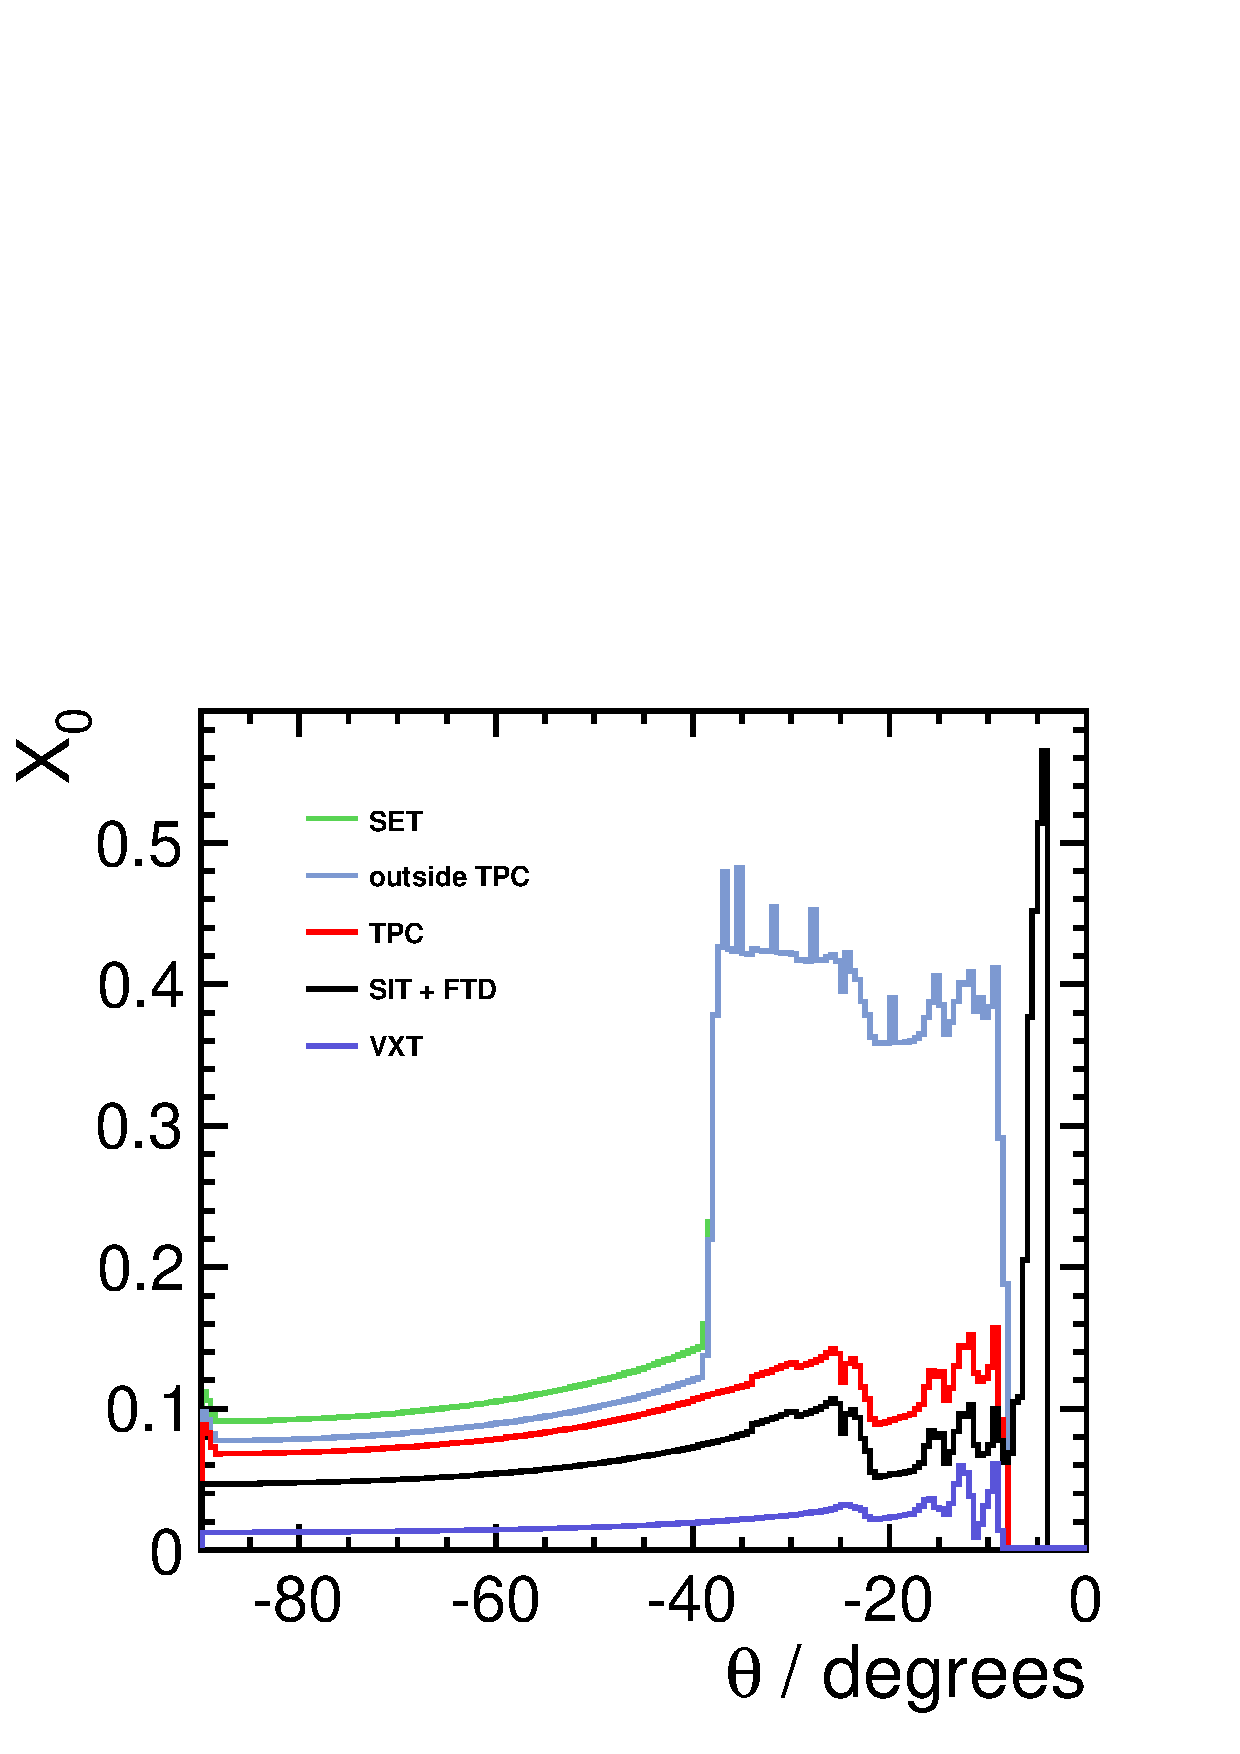
\includegraphics[width=0.52\hsize,viewport={0 -10 600 500},clip]{Introduction/fig/material-budget-new.pdf} &
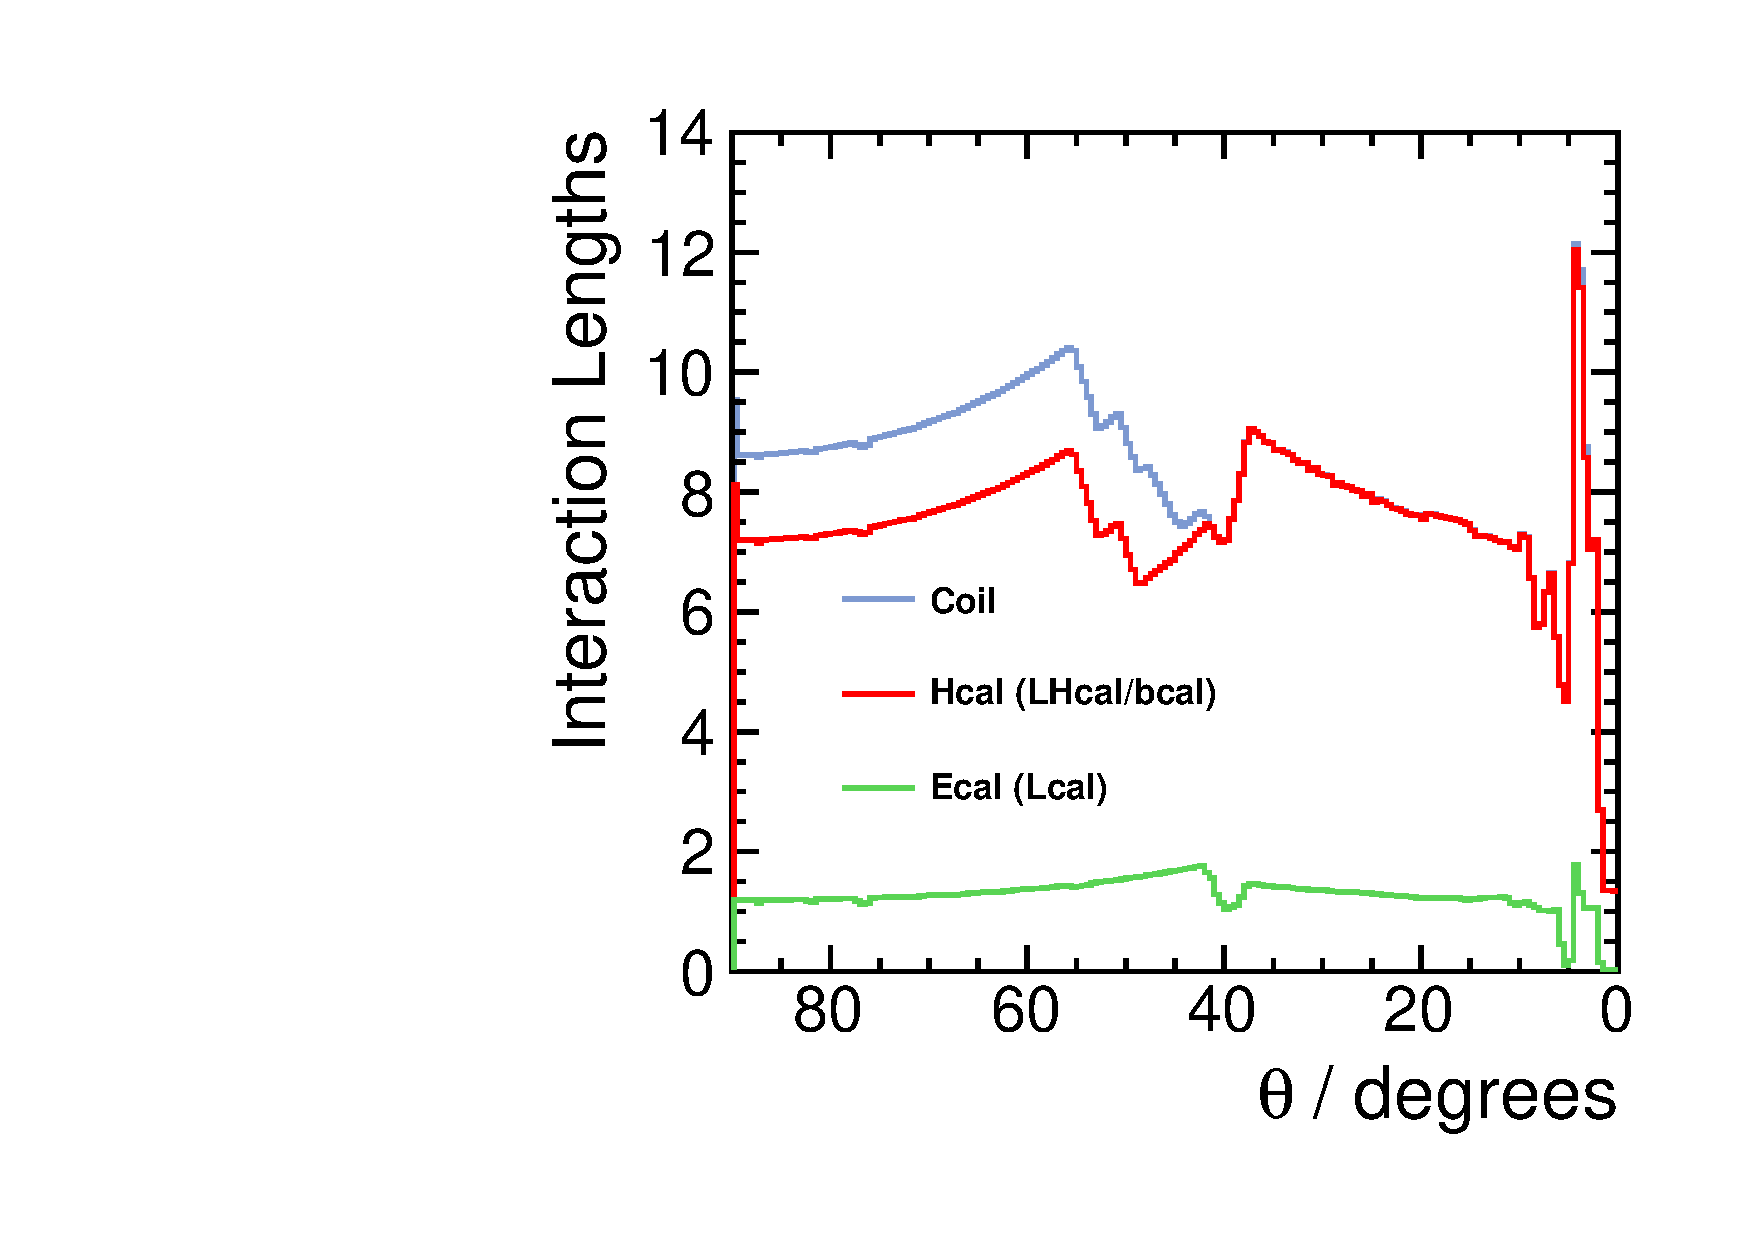
\includegraphics[width=0.5\hsize]{Introduction/fig/intlen_ILD_o1_v05.pdf}
\end{tabular}
\caption[Material in the ILD detector]{Left: Average total radiation length of the material
  in the tracking detectors as a function of polar angle. Right: Total interaction length in the detector, up to the end of the calorimeter system, and including the coil of the detector.}
%\end{figure}
\label{fig:intro:material}
%\begin{tabular}{cc}

\end{figure}


This is followed by a segmented hadronic calorimeter (HCAL) with up to 48 longitudinal samples and small transverse cell size. Two 
options are considered, both based on a Steel-absorber structure. One option uses scintillator tiles of $3 \times 3$\,cm$^2$, 
which are read out with an analogue system. The second uses a gas-based readout which allows a $1 \times 1$\,cm$^2$ 
cell geometry with a semi-digital readout of each cell. 

At very forward angles, below the coverage provided by the ECAL and the HCAL, a system of high precision and radiation hard calorimetric detectors (LumiCAL, BeamCAL, LHCAL) is foreseen. These
extend the calorimetric coverage to almost $4\pi$, measure the luminosity, and  monitor the quality of the colliding beams.

A large volume superconducting coil surrounds the calorimeters, creating an axial $B$-field of nominally 3.5-4\,Tesla.

An iron  yoke, instrumented with scintillator strips or resistive plate chambers (RPCs), returns the magnetic flux of the solenoid, and, at the same time, serves as a muon filter, muon detector and tail catcher calorimeter.

\thisfloatsetup{floatwidth=\SfigwFull,capposition=beside}
\begin{figure}[b!]
\begin{tabular}{cc}

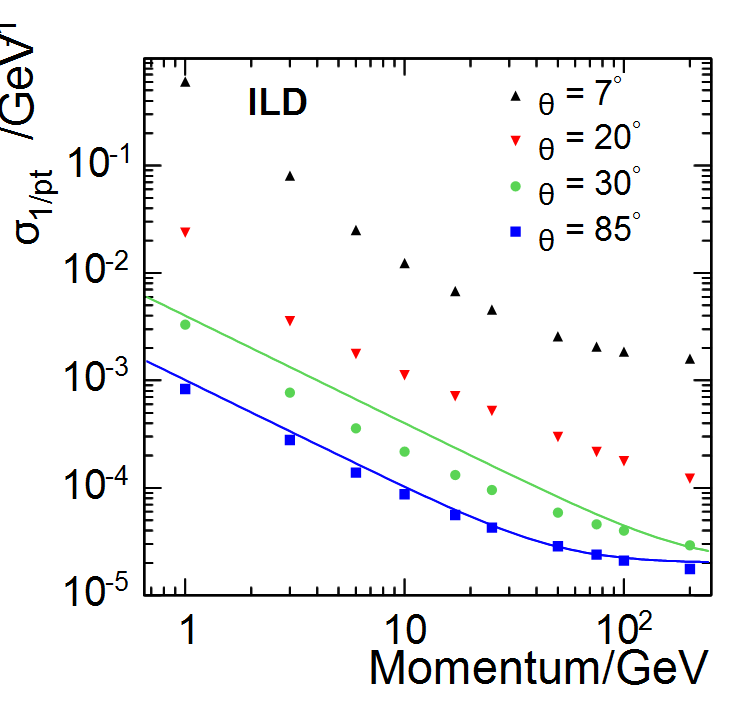
\includegraphics[width=0.5\hsize]{Introduction/fig/deltaInvP_all_fits.png} &
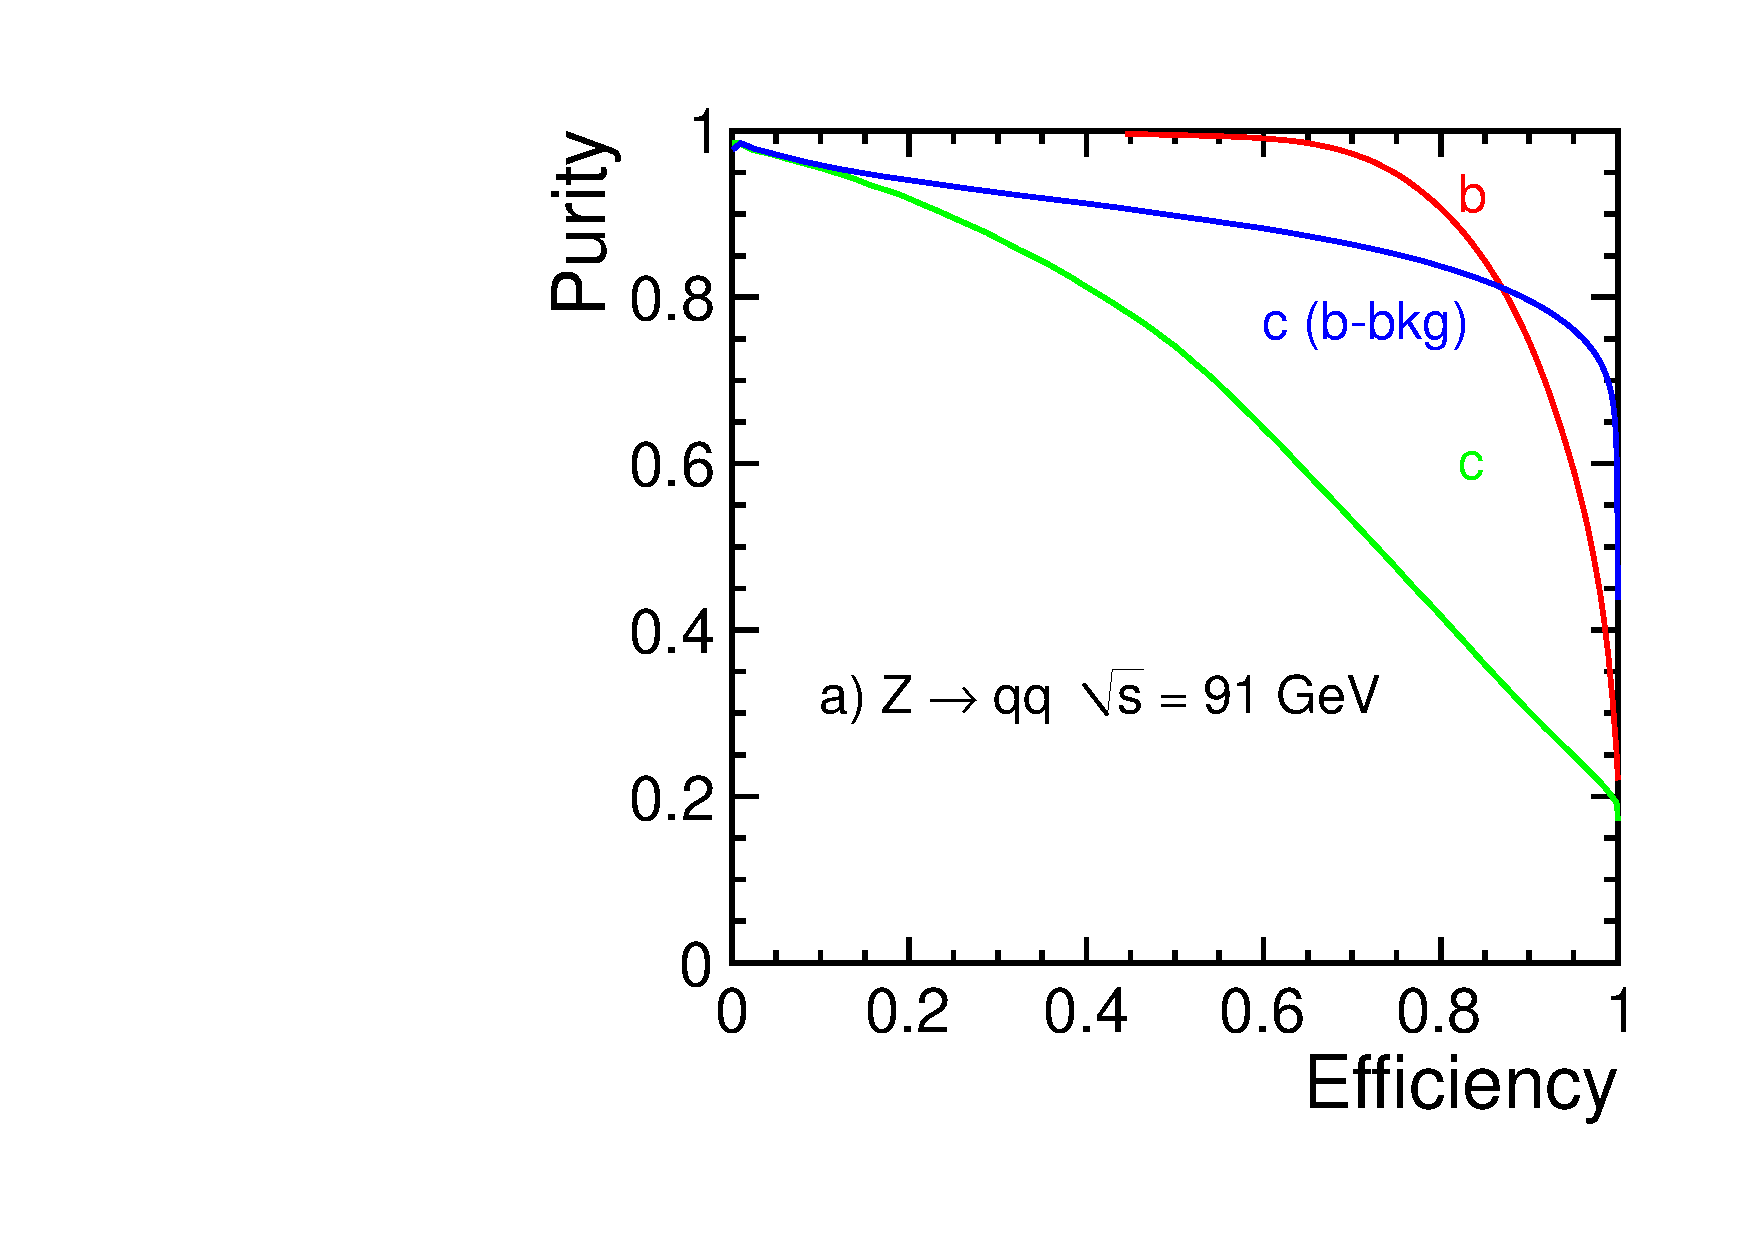
\includegraphics[width=0.5\hsize]{Introduction/fig/evalZ-lcfiweights_qq91new_v02-test.pdf}
\end{tabular}
\caption{\label{ild:fig:intro:tracking}(left) Momentum resolution for the ILD detector concept, as a function of the transverse momentum of the particle. (right) Flavour tagging efficiency versus purity for bottom events in sample of Z decays at 91\,GeV, and for charm events with only bottom background. )}
\end{figure}



\begin{figure}[t!]

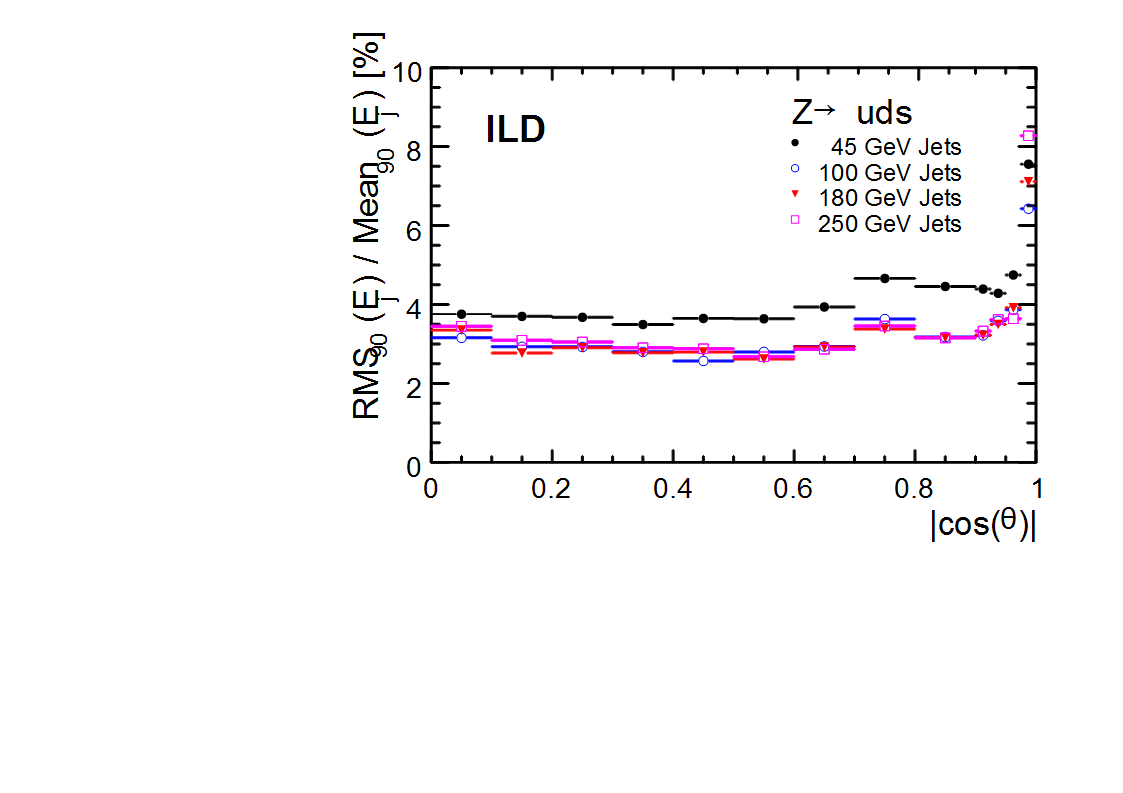
\includegraphics[width=0.8\hsize]{Introduction/fig/ild01_o1_pflow.png}

\caption{\label{ild:fig:intro:pflow}Fractional jet energy resolution
    plotted against $|\cos\theta|$ where theta is the polar angle of the thrust axis of the event. }
\end{figure}


The main parameters of the ILD detector are summarised in Table~\ref{ild:tab:barrelpara} and table~\ref{ild:tab:endcappara}.
%\begin{sidewaystable}[thb]
\begin{table}\hspace*{-0cm}\small
%\begin{tabular}{|l|p{0.8cm}p{0.8cm}p{1.0cm}|p{2.5cm}p{3.0cm}p{3.0cm}|}
%\begin{tabular}{|l|p{0.06\textwidth}p{0.06\textwidth}p{0.07\textwidth}|p{0.25\textwidth}p{0.20\textwidth}p{0.20\textwidth}|}
\begin{tabular}{ l p{0.05\hsize}p{0.04\hsize}p{0.04\hsize} p{0.20\hsize}p{0.20\hsize}p{0.20\hsize} }
%\hline
\toprule
\multicolumn{7}{l}{{\bf Barrel system}}\\
%\hline
\midrule
System & R(in) & R(out) & z & \multicolumn{3}{l}{comments}\\
       & \multicolumn{3}{c}{[mm]}   &&&\\
%\hline
\midrule
VTX    & 16         & 60        & 125 & 3 double layers &  Silicon pixel sensors, & \\
       &            &           &           & layer 1: & layer 2: & layer 3-6 \\
       &            &           &           & $\sigma<3 \mu m$ & $\sigma < 6 \mu m$ & $\sigma < 4 \mu m$ \\
Silicon &           &           & &&&\\
- SIT   & 153       & 300       & 644   & 2 silicon strip layers & $\sigma = 7 \mu m$& \\
- SET   & 1811      &           & 2300   & 2 silicon strip layers & $\sigma = 7 \mu m$& \\
- TPC   & 330       & 1808      & 2350   & MPGD readout & $1 \times 6 $mm$^2$ pads & $\sigma=60 \mu m$ at zero drift \\
%\hline
\midrule
ECAL    & 1843      & 2028      & 2350   & W absorber  & SiECAL & 30 Silicon sensor layers, $5 \times 5$ mm$^2$ cells \\
        &           &           &        &             & ScECAL & 30 Scintillator layers,  $ 5\times 45$ mm$^2$ strips \\
HCAL    & 2058      & 3410      & 2350   & Fe absorber & AHCAL & 48 Scintillator layers, $3 \times 3$cm$^2$ cells, analogue \\
        &           &           &         &            & SDHCAL & 48 Gas RPC layers, $1\times 1$ cm$^2$ cells, semi-digital\\
%\hline
\midrule
Coil    & 3440      & 4400      & 3950    & 3.5 T field & $ 2 \lambda $& \\
Muon    & 4450      & 7755      & 2800    & 14 scintillator layers& &\\
%\hline
\bottomrule
\end{tabular}
\caption{\label{ild:tab:barrelpara}List of the main parameters of the ILD detector for the barrel part.}
\end{table}

The performance of the ILD concept has been extensively studied using a detailed GEANT4 based simulation model and sophisticated reconstruction tools. Backgrounds have been taken into account to the best of current knowledge. 
A key characteristics of the detector is the amount of material in the detector. Particle flow requires a thin tracker, to minimise interactions before the calorimeters, and thick calorimeters, to fully absorb the showers. Figure~\ref{ild:fig:intro:material}~(left) shows the material in the detector in radiation lengths, until the entry of the calorimeter. The right plot shows the total interaction length including the calorimeter system. 

The performance of the tracking system can be summarised by its combined momentum resolution, shown in Figure~\ref{ild:fig:intro:tracking}~(left). A resolution of $\sigma_{1/p_T} = 2 \times 10^{-5}$\,GeV$^{-1}$ has been achieved for high momenta. For many physics studies the tagging of long lived particles is of key importance. Several layers of pixel detectors close to the IP allow the reconstruction of displaced vertices, as shown in Figure~\ref{ild:fig:intro:tracking}~(right).



%\begin{table}\hspace*{-2.5cm}\small
%\begin{tabular}{|l|p{0.8cm}p{0.8cm}p{1.0cm}|p{2.7cm}p{3.7cm}p{3.7cm}|}

\begin{table}\hspace*{-0cm}\small
%\begin{tabular}{|l|p{0.8cm}p{0.8cm}p{1.0cm}|p{2.5cm}p{3.0cm}p{3.0cm}|}
\begin{tabular}{ l p{0.05\hsize}p{0.04\hsize}p{0.04\hsize} p{0.20\hsize}p{0.20\hsize}p{0.20\hsize} }

%\hline
\toprule
\multicolumn{7}{ l }{{\bf End cap system}}\\
\midrule
System & z(min) & z(max) & r(min), r(max) & \multicolumn{3}{l}{comments}\\
       & \multicolumn{3}{c}{[mm]}   &&&\\
\midrule

FTD    & 220     & 371    &      & 2 pixel disks & $\sigma=2-6 \mu m$ &\\
       &         &        &      & 5 strip disks & $\sigma = 7 \mu m$& \\
ETD    & 2420    & 2445   & 419-1822 & 2 silicon strip layers & $\sigma=7 \mu m$ & \\
\midrule
ECAL   & 2450    & 2635   &      & W-absorber & SiECAL & Si readout layers \\
       &         &        &      &            & ScECAL & Scintillator layers \\
HCAL   & 2650    & 3937   & 335-3190& Fe absorber & AHCAL & 48 Scintillator layers $3 \times 3 $cm$^2$ cells, analogue\\
       &         &        &      &              & SDHCAL & 48 gas RPC layers $1\times 1$cm$^2$ cells, semi-digital \\
BeamCal & 3595   & 3715   & 20-150  & W absorber& 30 GaAs readout layers & \\
Lumical & 2500   & 2634   & 76-280 & W absorber & 30 Silicon layers & \\
LHCAL   & 2680   & 3205   & 93-331 & W absorber &&\\
\midrule
Muon    & 2560   &        & 300-7755 & 12 scintillator layers&&\\
\bottomrule
\end{tabular}
\caption{\label{ild:tab:endcappara}List of the main parameters of the ILD detector for the end cap part.}

\end{table}

Calorimeter system and tracking system together enter into the particle flow performance. The performance of the ILD detector for different energies and as a function of the polar angle is shown in Figure~\ref{ild:fig:intro:pflow}. 

The few plots shown in this introduction illustrate the anticipated performance of the detector and illustrate the potential for precision measurements with the ILD detector. More details on the performance may be found in section~\ref{ild:sec:performance} of this document. 

In this document the current state of the design of the ILD detector is summarised. The technologies which are proposed for the different parts of the detector are introduced. An extensive benchmarking has been performed, to demonstrate the performance of the ILD detector. This has been done for two different detector implementations, a large and a smaller one. Both concepts are the result of intense optimization efforts, with different goals - cost effectivnes was foremost a criterium for the smaller one, ultimate performance for the larger model. 

The ILD group who is proposing this detector has currently some 70 member institutes from all around the world. The group has evolved into a proto-collaboration, which is positioning itself to move forward with a proposal for a detector at the ILC at the moment that ILC becomes a real project. 

A lot of the work presented in this report is based on intense R\&D work which has taken place over the last decade to develop the necessary technologies. 
This work has typically happened within dedicated R\&D collaborations, which are independent but maintain very close connections to ILD. All technologies selected by ILD for one of its subsystems have been proven experimentally to meet the performance goals, or to come very close. 

Developing a very powerful detector concept over a long period of time requires balancing cutting edge technologies, which might become available while the concept is being developed, with safe and sound solutions. ILD in many cases is pursuing more than one technological option, to remain flexible and to be able to adopt to new developments. The concept group  wants to remain open and flexible to be prepared to select the most modern and most powerful technology once it is necessary. 
However a distinction is made between options and alternatives: while options have undergone an extensive R\&D program and have passed critical proof-of-concept tests, alternatives are potentially interesting and promising technologies which have not matured to a similar level at the time of writing this document. 

The following document starts with a short review of the science goals of the ILC, and how the goals can be achieved today with the detector technologies at hand. After a discussion of the ILC and the environment in which the experiment will take place the detector is described in more detail. The integration of the different sub-systems into an integrated detector is discussed, as is the interface between the detector and the collider. This is followed by a concise summary of the benchmarking which has been performed in order to find an optimal balance between performance and cost. To this end the costing methodology used by ILD is presented, and a cost estimate for the detector in 2018 costs is presented. The report closes with a summary of the proposed detector and its performance. 
\chapter{The ILC Environment}

\writer{Karsten Buesser, Keisuke Fujii}{3}
\chapter{The ILD detector concept}
%\writer{Ties Behnke, Kiyotomo Kawagoe, Claude Vallee}{}
\label{chap:ILD}

\section{The overall ILD concept}

The overall ILD concept has been kept unchanged since the DBD~\cite{ild:bib:ilddbd}. The detector global layout and the performance of the subdetectors are tightly linked to the accelerator characteristics and the physics requirements, as summarised in figure ~\ref{fig:ILD:specifications}. 

The high beamstrahlung background at the collision point requires a magnetic field higher than 3\,T to confine most of the low-energy electron pairs  within the beam pipe, and sets a minimum of $\approx$1.5~cm for the closest distance of approach of the vertex detector inner layer from the beamline. On the other hand the bunch structure of short trains separated by long idle periods sets rather relaxed conditions on the data acquisition, with the possibility to avoid a hardware trigger system. This in addition allows to power the front-end electronics only during active bunch trains (so-called "power-pulsing" mode), which minimises the subdetector cooling requirements and associated material budgets.  

The subdetector specifications are tightly linked to the physics requirements from precision Higgs and electroweak physics. The dominant Higgs strahlung process, which at an $e^+e^-$ collider provides the unique opportunity to tag Higgs production independently of Higgs decay mode, requires a very high-precision momentum measurement of isolated particles from Z decays and hence a high precision main tracker. The efficient tagging of quark and lepton flavours to disentangle Higgs couplings requires a very high precision and low-material vertex detector, which also improves on the particle momentum measurements, as well as a high calorimeter granularity to identify leptons in jets. Similarly an efficient identification of W, Z and top hadronic decays in a crowded multijet environment needs a high jet energy resolution, twice better than currently realized at LHC, as well as an efficient spatial jet separation. ILD considers that the best concept to meet these requirements altogether is particle flow, where the charged and neutral particle contents of the jets are measured with the high performance trackers and the high granularity calorimeters, respectively. Within this scheme, an efficient match between the trackers and the calorimeters requires the calorimeters to be positioned inside the coil.     

\begin{figure}[t!]
\centering
%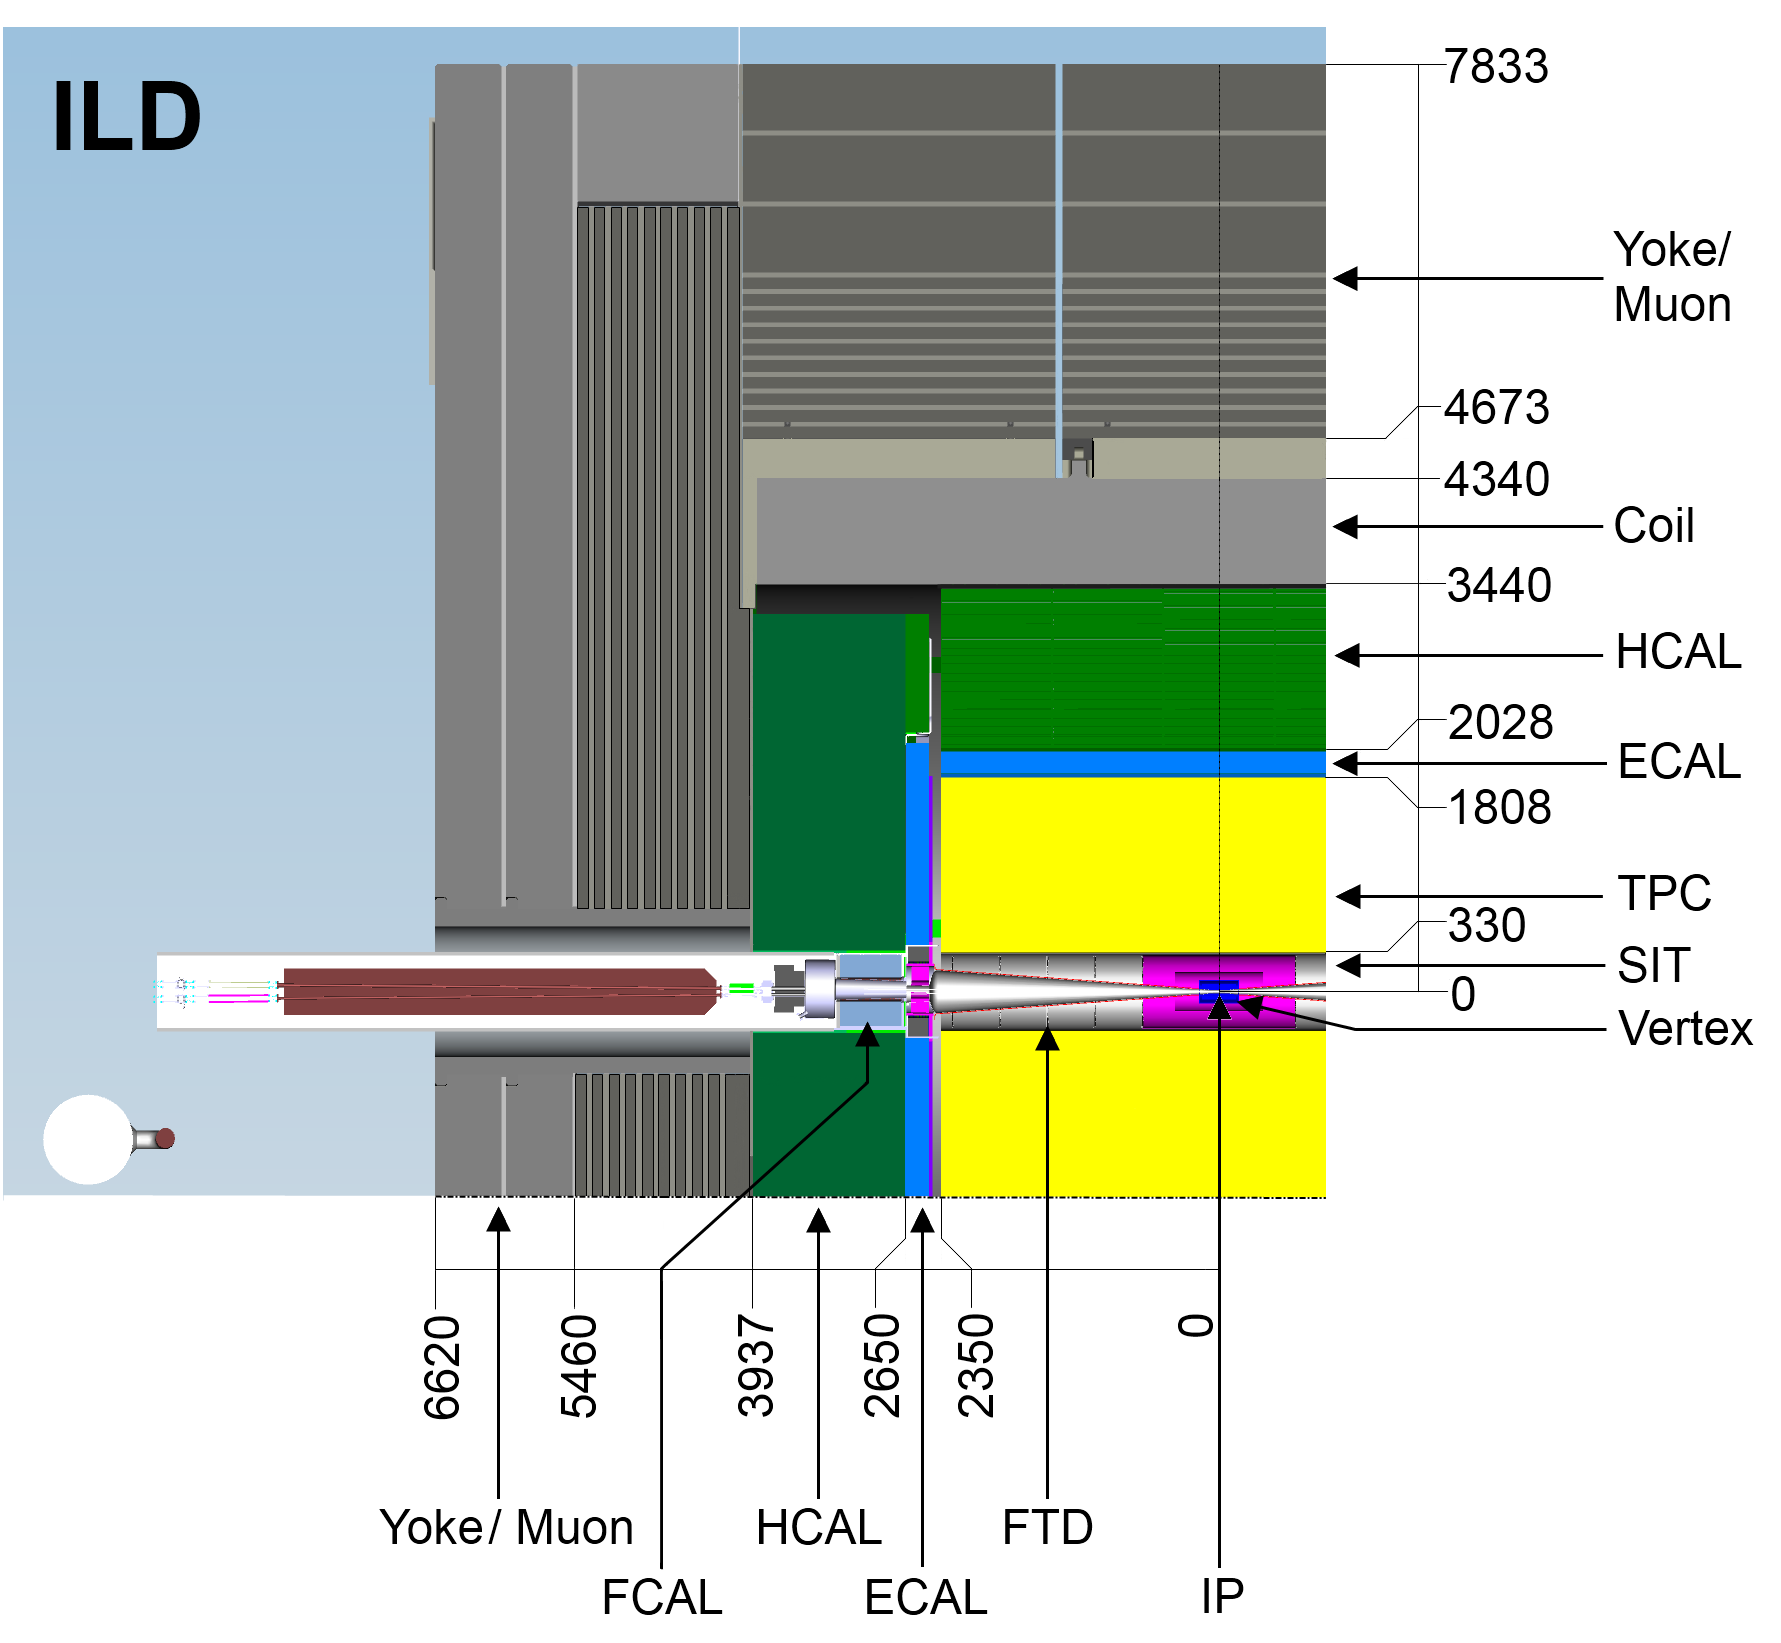
\includegraphics[width=0.8\hsize]{Detector/fig/ILD_quadrant_2.png}
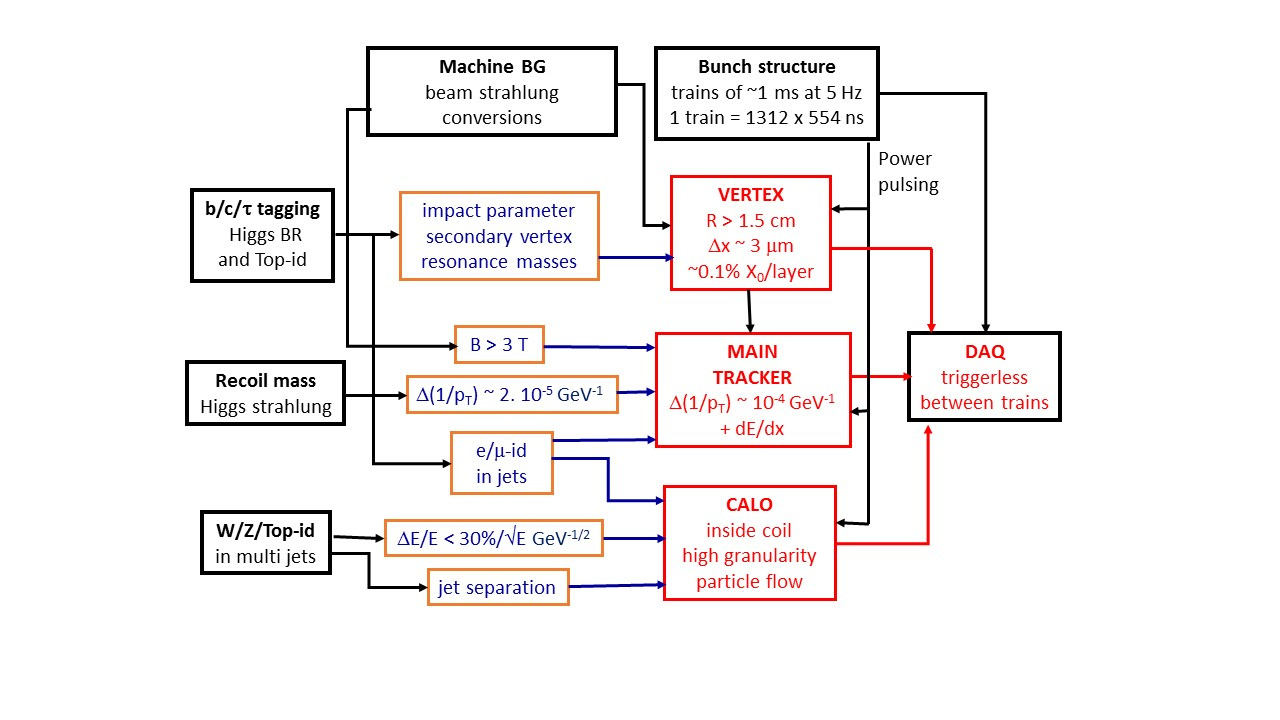
\includegraphics[width=1.0\hsize]{ILD/fig/ILD_specifications.jpg}
\caption{Interplay between ILC machine characteristics, physics requirements and detector specifications.}
\label{fig:ILD:specifications}
\end{figure}
%\textit{Detector performance aspects to be anticipated for higher energies}


\section{Optimizing ILD}

The baseline ILD layout of the DBD~\cite{ild:bib:ilddbd} had intentionally large dimensions in order to maximize the tracking performance and the particle flow capabilities of the calorimeters. The main cost drivers of the DBD detector were the electromagnetic calorimeter and the coil/yoke system, for which specific options are considered to reduce their costs (chapters 6.4 and 9). In the past years a re-optimization process of the detector global dimensions has been launched to identify an optimal point in the cost-performance space.

In a first step, a parametric study \cite{Ref:bib:TPCOPT} of the dependence of cost and performance as function of the outer radius and length of the main tracker (the TPC in ILD) has been performed. 
A simple model has been constructed, based on the cost estimate published as part of the ILD DBD~\cite{ild:bib:ilddbd}. In this model the cost of each subdetector is scaled as a function of the size based on simple scaling laws. Sensitive detector elements like Silicon planes are scaled with the total area, while mechanical elements - for example, the absorber in a calorimeter - scale with the volume. The reference is always the DBD cost estimate. To study the effect of changing the TPC radius and length, all other dimensions outside of the TPC are tied to the TPC radius and TPC length. Clearances between detectors are kept constant, and do not scale. In this way, an overall cost scaling of the ILD detector can be computed, which is probably correct at the level of 10-20\%. 

The performance of the detector is measured by a combined performance estimator, based on a few observables mostly from Higgs physics. Essentially, these are the tracking performance (momentum resolution and impact parameter resolution), the Higgs mass precision (with and without Beam-Strahlungs background), the inverse of the significance of b-tagging, and the minimum $p_t$ to reach the last layer of the vertex detector. All numbers are normalised to the performance of the DBD detector. For a more complete description of the method and the definitions, see \cite{Ref:bib:TPCOPT}. 

Two types of iso-curves are then defined in the space opened by the TPC radius and length: Equal performance, and equal cost. In figure ~\ref{fig:ILD:aspect_ratio} iso-cost and iso-performance curves are shown. The three red lines correspond to costs relative to the DBD of (from top to bottom) 100\%, 90\% and 80\%. The blue lines indicate equal-performance lines. From the plot it can be seen that the dependence of the cost on the detector radius is steeper than on the length, while the performance scales roughly the same for both. This shows that targeting a given cost reduction maintains a higher performance when reducing the radius while keeping the overall length unchanged, instead of keeping the aspect ratio r/z unchanged.  

\begin{figure}[t!]
\centering
%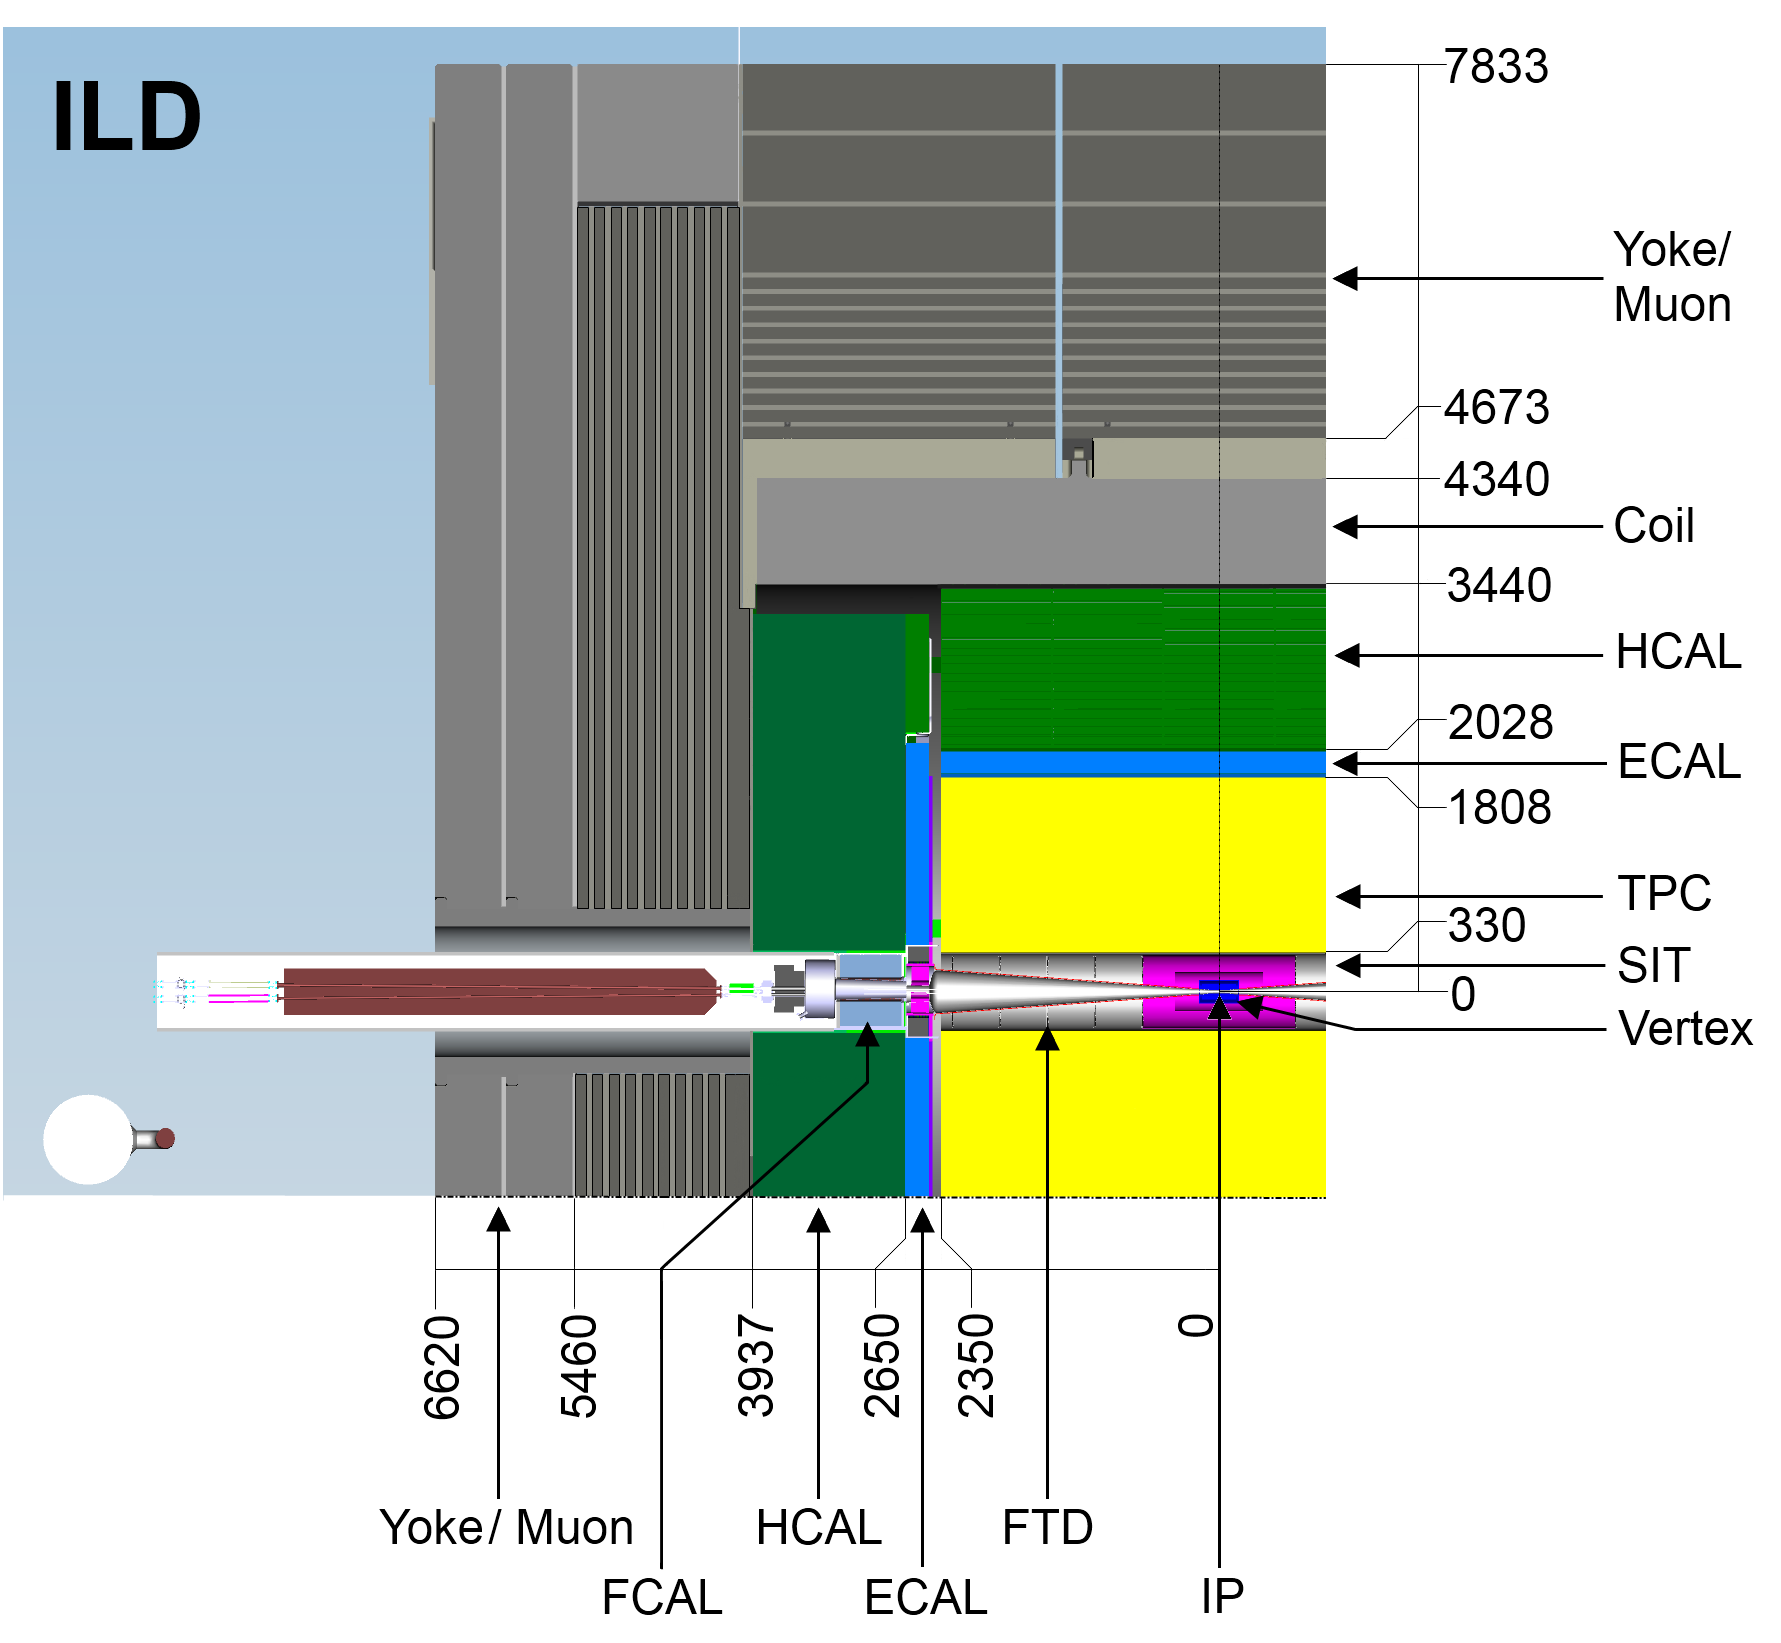
\includegraphics[width=0.8\hsize]{Detector/fig/ILD_quadrant_2.png}
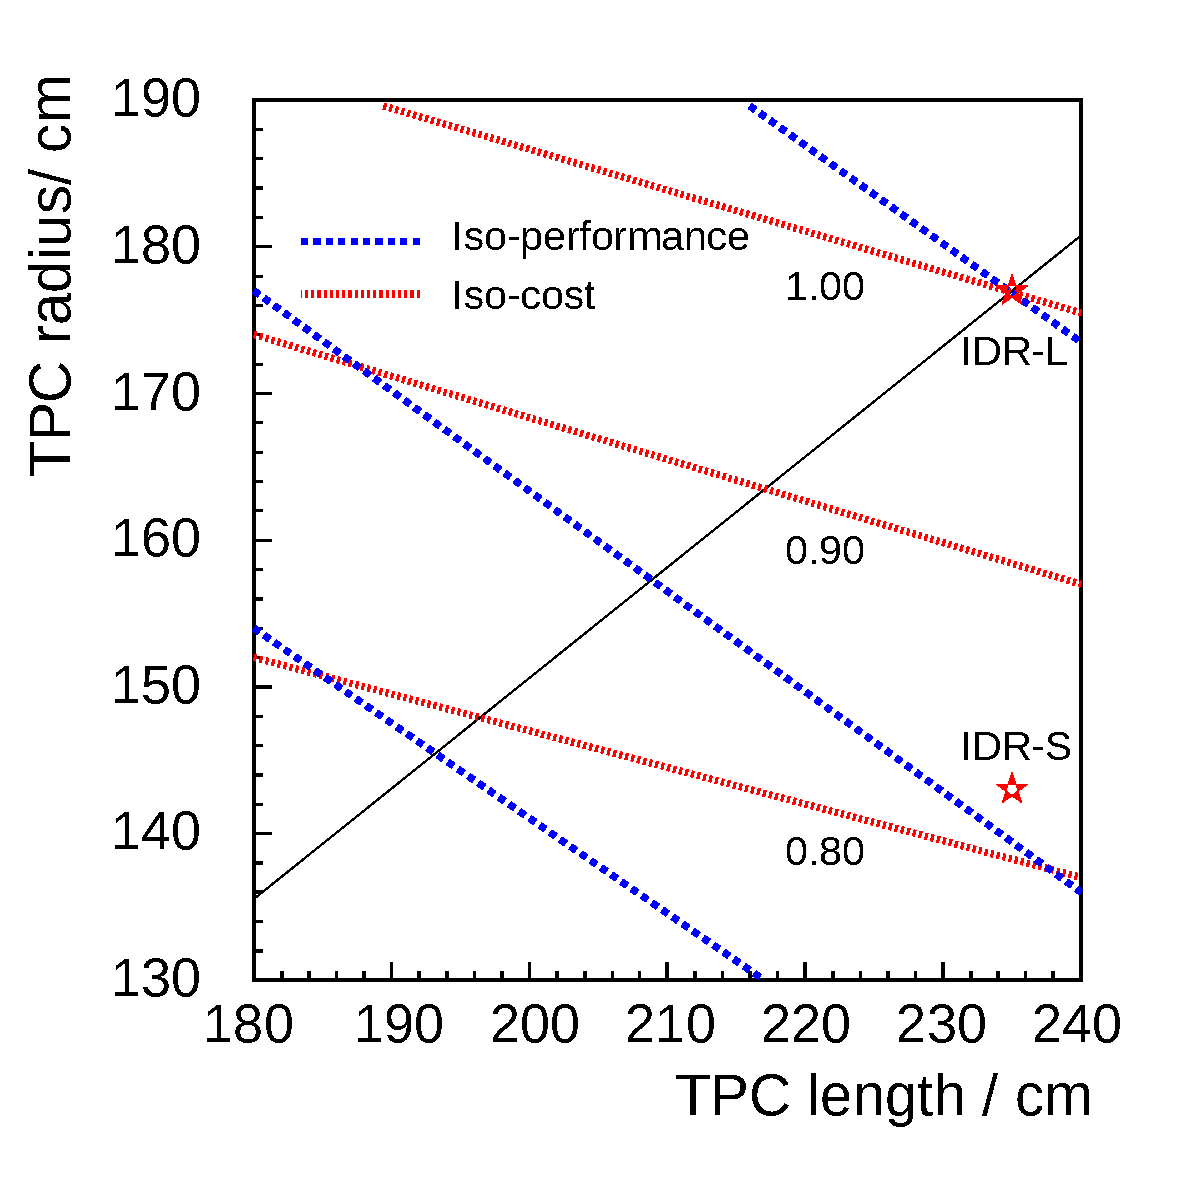
\includegraphics[width=0.5\hsize]{ILD/fig/aspect_ratio.pdf}
\caption{Iso-performance and iso-cost curves resulting from a parametric evaluation of the ILD detector in the tracker radius-length parameter space. The stars indicate the location of the different ILD models in this parameter space. The black diagonal line indicates dimension changes at a constant r/z aspect ratio.}
\label{fig:ILD:aspect_ratio}
\end{figure}

Based on this study, detector models with different sizes were defined with the following guidelines:

\begin{itemize}
    
\item The number of detector models is limited to two to maintain simulations and analyses at a manageable level.

\item One of the models ("IDR-L") has dimensions similar to those of the DBD model, in order to have a well understood reference in the studies. The only changes compared to the DBD are associated to the collider parameter evolution (e.g. the new L* optics, see chapter 3), and to better understanding of the subdetector technology constraints. This resulted in small changes to the TPC outer radius and length. 

\item The second model ("IDR-S") has a reduced outer radius of the main tracker while keeping its length unchanged. The smaller radius has to be far enough from the IDR-L radius to provide a significant lever-arm for the comparison. The chosen value is equal to that of the new CLIC detector model CLICdp~\cite{Arominski:2018uuz}, half way of the even smaller radius of the SiD detector~\cite{ild:bib:ilddbd}. With this choice IDR-S has similar outer tracker dimensions to CLICdp for both radius and length. This offers the possibility to compare the performance of the TPC option to the all-silicon option favored by CLICdp. 

\item All other components of IDR-S are similar to IDR-L. The inner tracking and very forward detectors are identical. The calorimeter depths and cell sizes are also kept unchanged, and the number of cells is reduced only as function of the calorimeter radii. All external systems such as coil, yoke and endcaps have their radial dimensions reduced accordingly.

\item In order to compensate for the smaller tracking lever-arm the nominal magnetic field of IDR-S is increased from 3.5\,T to 4\,T.

\end{itemize}

\begin{figure}[t!]
\centering
%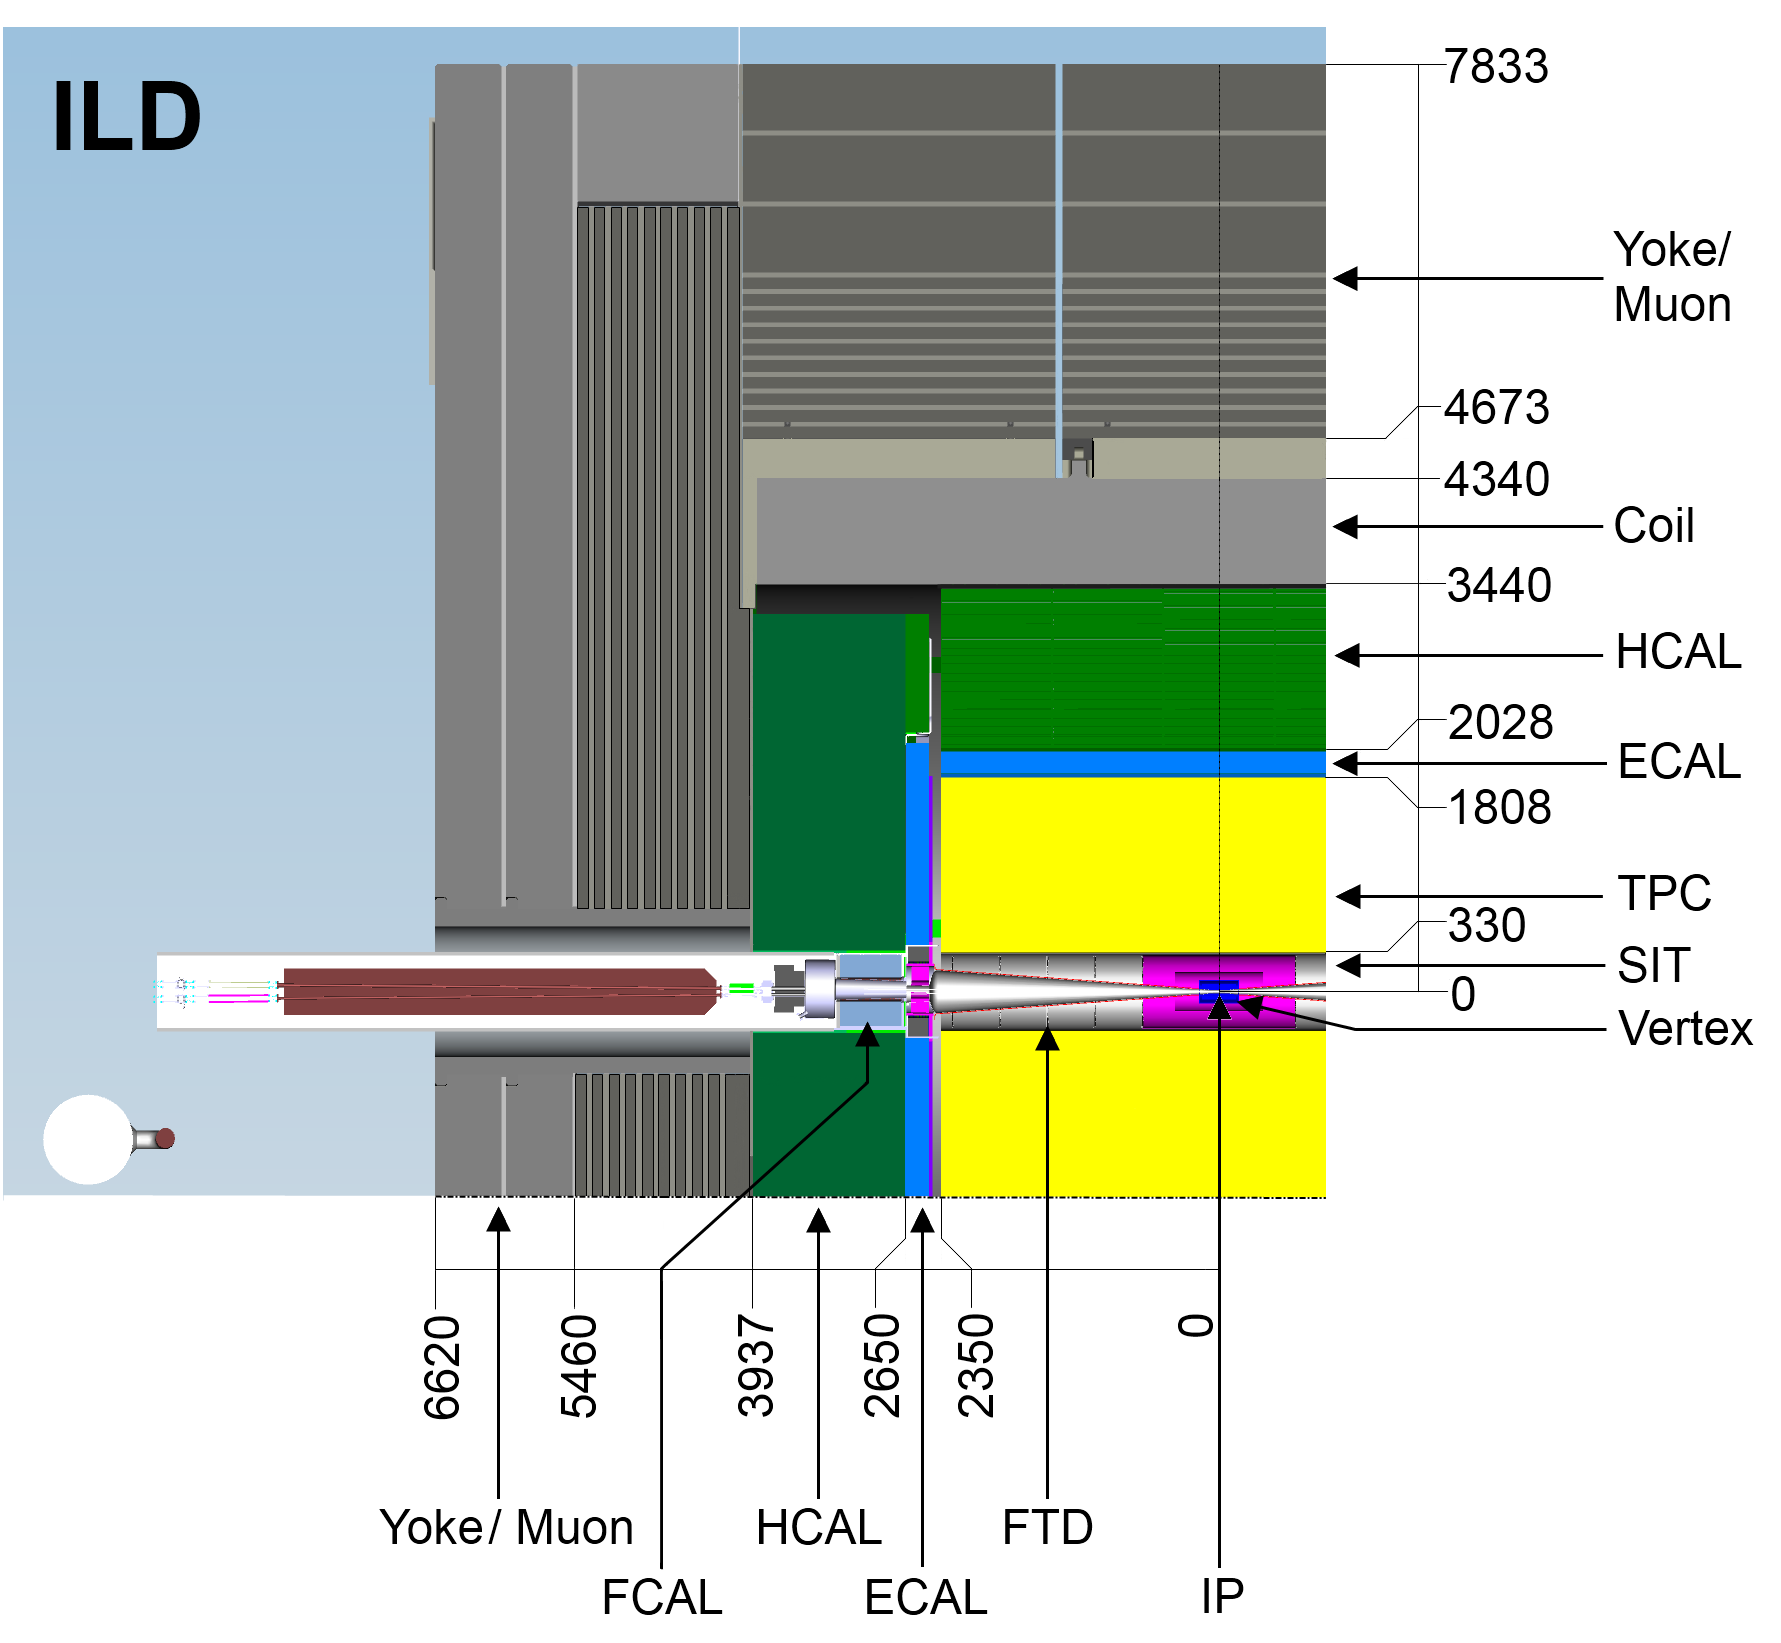
\includegraphics[width=0.8\hsize]{Detector/fig/ILD_quadrant_2.png}
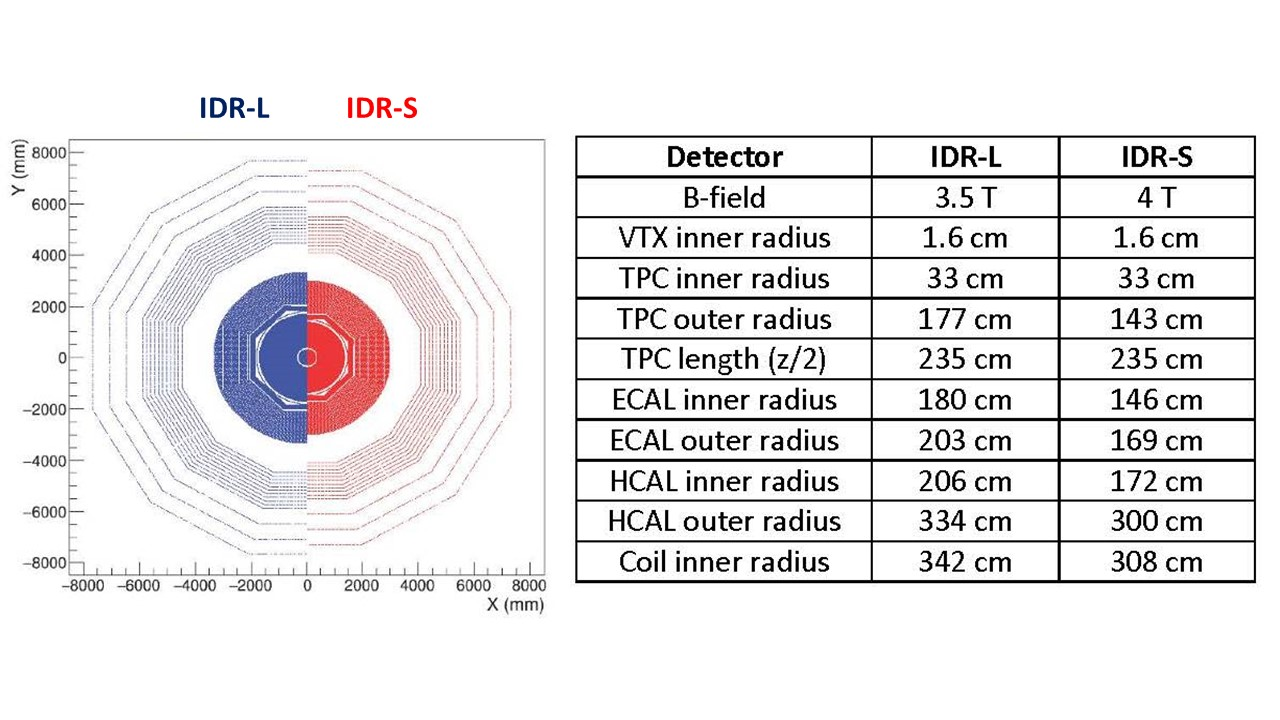
\includegraphics[width=1.0\hsize]{ILD/fig/ILD_small-large.jpg}
\caption{The large ("IDR-L") and small ("IDR-S") models used for the ILD optimization: R-$\phi$ view (left) and main subdetector dimensions (right).}
\label{fig:ILD:sizes}
\end{figure}

The resulting IDR-L and IDR-S dimensions are summarised in figure ~\ref{fig:ILD:sizes}. Both models were used for detailed simulations of physics benchmark samples. The simulation framework is described in chapter~\ref{chap:modelling}. The detector and physics performance of both models are compared in chapter~\ref{chap:performance} and their costing estimated in chapter~\ref{chap:costing}. \vfill


	
\chapter{Detector Layout and Technologies}

\section{Overall structure of the detector}
\writer{Claude Vallee, Karsten Buesser}{1}
\vspace{4cm}
\subsection{Global structure and parameters}
\writer{Claude Vallee, Karsten Buesser}{1}

Reminder of the global structure of the ILD detector, focusing details on the main changes since DBD, and mentioning remaining open options like anti-DID.

\vspace{2cm}
\subsection{Subdetecor layouts}
\writer{Subdetector technical conveners}{4}

Description of the latest baseline design of subdetectors, including open options. Each technology option description should indicate its advantages (pro) and critical aspects (cons) in respect to ILD specifications. Potential new capabilities for the future (e.g. calorimeter timing) should also be indicated.

Vertex detector (Besson, Ishikawa, Vos): nb layers, dimensions, technology options.

Internal silicon trackers (Besson, Vos, Vila): FTD disks, dimensions, technology per disk, SiT including pixel option, short discussion status
outer TPC  silicon layers

TPC (Colas, Sugiyama): structure and readout options (GEM, Micromegas)

ECAL (Brient, Ootani): mechanical layout and readout options (Si, Sc)

HCAL (Laktineh, Sefkow): mechanical options (Videau,TESLA_ and readout options (Sc, RPC)

VFS (Benhammou, Schuwalow): layout adapted to new L*, LUMICAL, BEAMCAL,LHCAL sensors

Iron instrumentation (Saveliev): sensitive layers in yoke baseline design and sensor structure

\vspace{2cm}
\section{Subdetector technology status}
\writer{Subdetector conveners}{}

This section is one of the main technical added values of the IDR. It should summarize all technological progress since the DBD, including beam tests of technological prototypes and ongoing spinoffs. It should also indicate the remaining steps to fulfil the ILD requirements, with a focus of critical aspects associated to each technology choice. For conciseness only the highlights should be illustrated, with all details to be referenced in technical publications. As regards illustrations it is proposed to stick to o(1-2) photo and o(1-2) plot  for each technology. 

\vspace{2cm}
\subsection{Vertex detector}
\writer{Auguste Besson, Akimasa Ishikawa, Marcel Vos}{3}

CMOS spin-offs: ALPIDE (ALICE upgrade) and MIMOSIS (CBM), New PSIRA chip for ILD

DEPFET spin-off: BELLE-2, BEAST and first physics events

FPCCD long prototype and irradiation tests

Short mention of other options:  SOI, etc

Low material support developments (PLUME ladder) and cooling studies

\vspace{2cm}
\subsection{Silicon inner tracking detectors}
\writer{Marcel Vos, Ivan Vila}{1}

Above DEPFET developments and FTD thermo-mechanical mockup

\vspace{2cm}
\subsection{Time projection chamber}
\writer{Paul Colas, Akira Sugiyama}{3}

TPC prototype for generic beam tests of all readout options, the gating scheme and cooling. Mention LYCORIS silicon telescope and new field cage in construction.

CO2 Cooling measurements            

Successful gating achieved with GEM

GEM and Micromegas spacial and ionization resolutions

Ongoing technological developments: improved module planarity, GRIDPIX RO options, etc.  

\vspace{2cm}
\subsection{Calorimeters}
\writer{Jean Claude Brient, Wataru Ootani, Felix Sefkow, Imad Laktineh}{5}

Si-ECAL: technological prototype (incl long slab) beamtest results, CMS HGCAL spinoff.

Sc-ECAL results from new detector unit in construction.

AHCAL beamtest results from large technological prototype, CMS HGCAL spinoff.

SDHCAL beamtest results of large technological prototype at CERN, ongoing development of large chambers. 

\vspace{2cm}
\subsection{Very forward detectors}
\writer{Yan Benhammou, Sergej Schuwalow}{2}

LUMICAL sensors: Beam test of thinner prototypes with improved transverse resolution of e-showers

BEAMCAL and LHCAL developments

\vspace{4cm}
\subsection{Iron instrumentation}
\writer{Valery Saveliev}{1}

Fermilab Scintillator detectors prototypes and performance tests

\vspace{2cm}
\chapter{ILD Global Integration}
\writer{Karsten Buesser, Claude Vallee}

\vspace{2cm}
\section{External ILD integration}
%\writer{Yasuhiro Sugimoto}{1}
\label{ild:sec:external_integration}
%Generic layout of the cavern, mentioning the current options for its configuration (TDR, Tohoku, YS).

The proposed site for the ILC is located in the Kitakami mountains in the north of the Japanese main island Honshu. Dedicated studies are under way to adapt the generic ILC design, as described in the Technical Design Report, to the realities in this environment. For ILD, the arrangements of the surface and underground installations around the interaction point (IP) are of natural importance. The current conceptual design of the civil facilities and the plans for the detector related infrastructure and services have been coordinated between the relevant detector and ILC machine groups as well as with local experts.

\subsection{Site-related Infrastructure}

ILD is foreseen to be assembled on the surface, similar to CMS at LHC. Figure~\ref{fig:integration:surface} shows a rendering of the surface installations above the ILC interaction point. At the heart is the detector assembly building that is located directly over the central shaft that gives access to the underground collider hall. A large gantry crane above the shaft allows for the lowering of the pre-instrumented detector parts into the underground area. A preparation building is foreseen where sub-detector elements can be assembled and tested. A research building and a computing building provide the infrastructure for the operation of the detectors at the IP Campus. 

\begin{figure}[htbp]
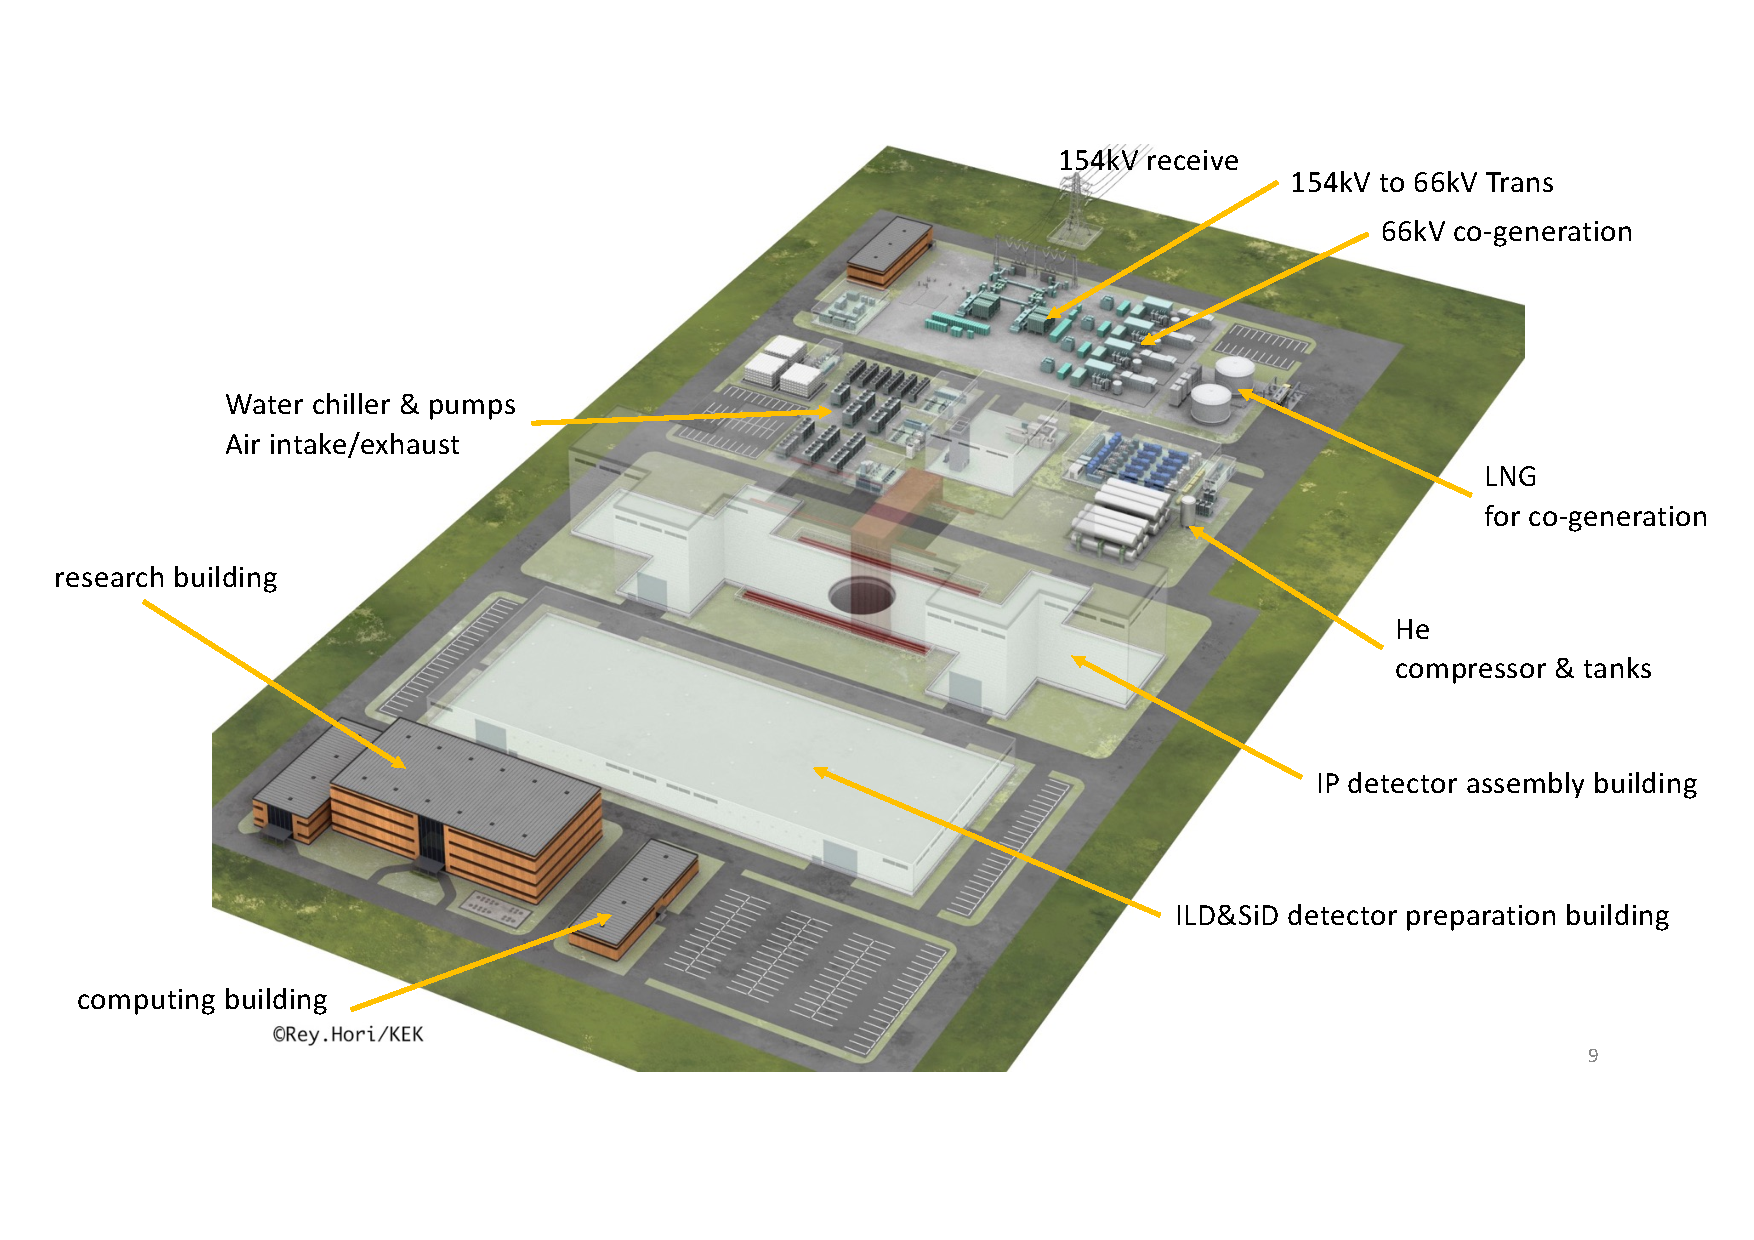
\includegraphics[width=0.9\hsize]{Integration/fig/Surface_Facilities.pdf}
\caption{\label{fig:integration:surface}Conceptual design (artist's view) of the surface facilities ("IP Campus") above the ILC interaction point~\cite{ild:bib:surface_facilities}. }
\end{figure}

The underground experimental hall is about 100~m below the surface and hosts two experiments, ILD and SiD, in a "push-pull" arrangement where both detectors share the same interaction region (c.f.~Figure~\ref{fig:integration:underground}). The detectors are installed on movable platforms and can be rolled into or out of the beam line within a few hours. They can be opened and maintained in their parking positions. Access to the underground hall is provided by two vertical shafts and an access tunnel that allows for vehicles to drive directly into the underground area, c.f.~Figure\ref{fig:integration:access}.

\begin{figure}[h!]
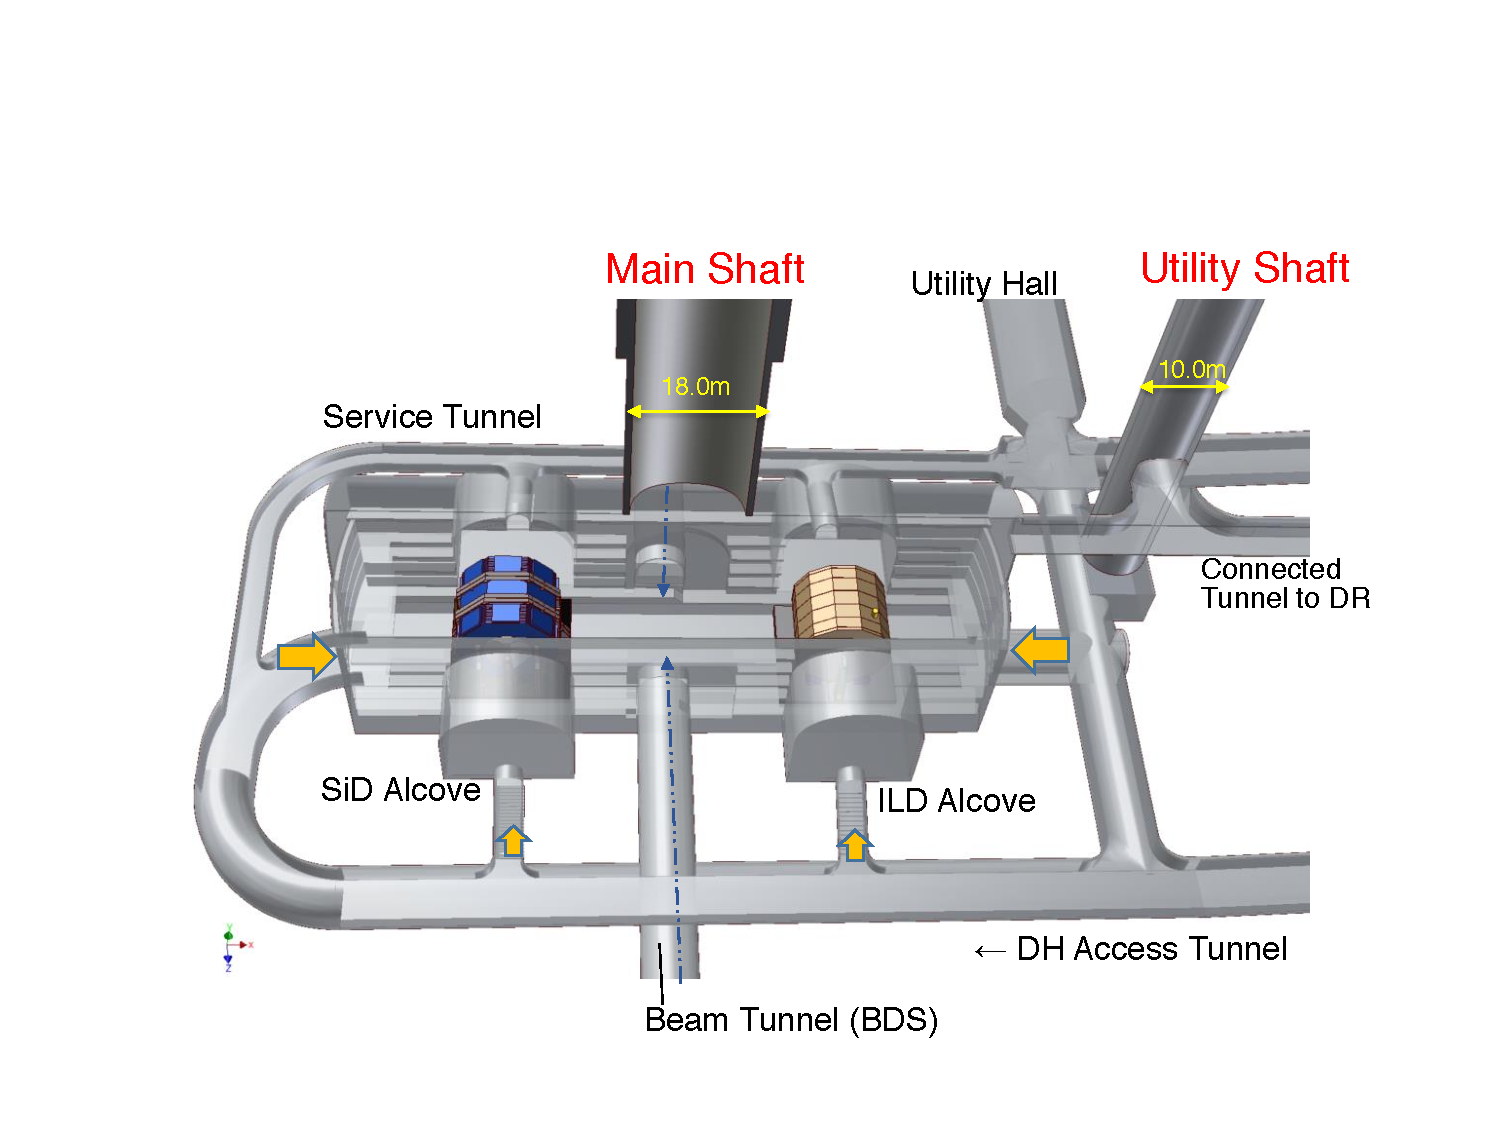
\includegraphics[width=1.0\hsize]{Integration/fig/Underground_Facilities.pdf}
\caption{\label{fig:integration:underground}Underground facilities with the detector hall, ILD and SiD in push-pull configuration, access tunnels and shafts~\cite{ild:bib:underground_facilities}. }
\end{figure}


\begin{figure}[h!]
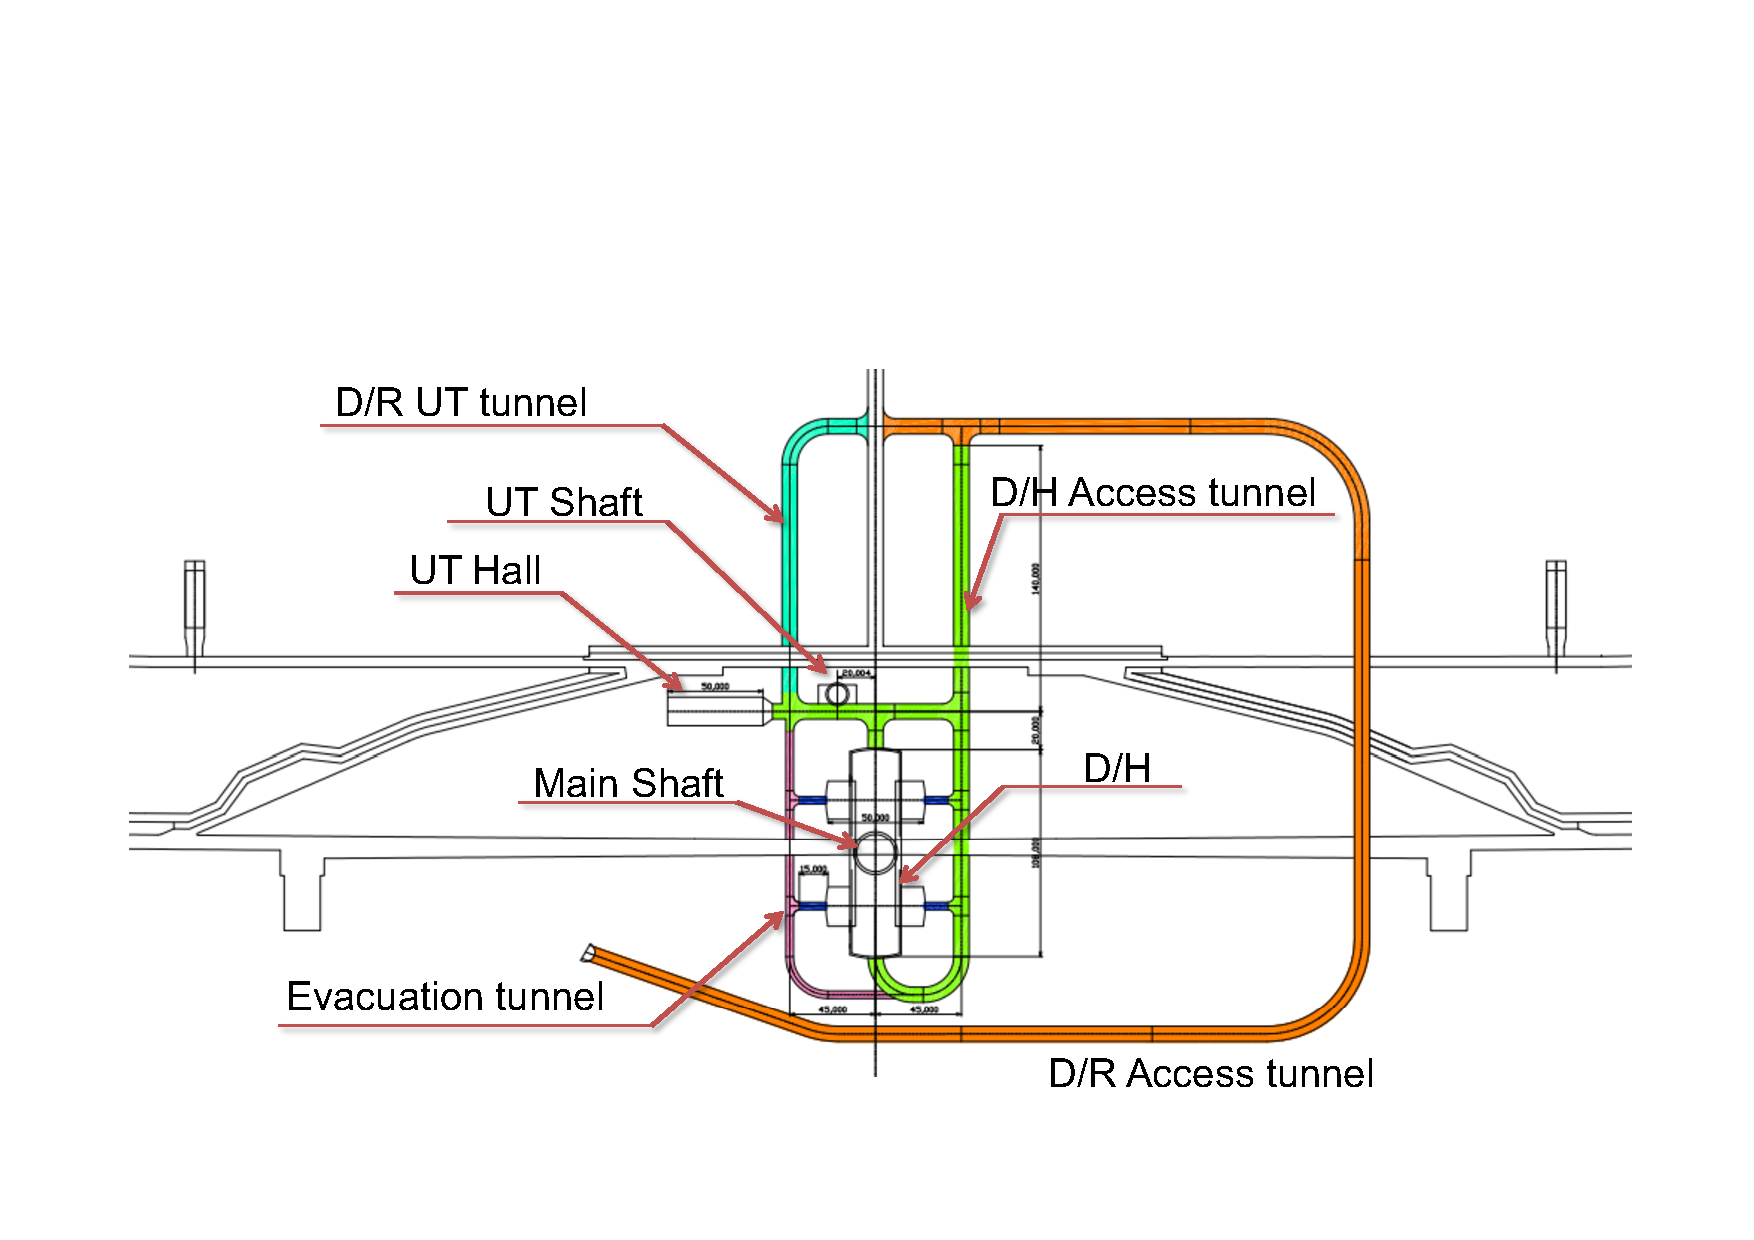
\includegraphics[width=1.0\hsize]{Integration/fig/Access.pdf}
\caption{\label{fig:integration:access}Access to the underground infrastructure is provided by two shafts, main shaft and utility (UT) shaft, and a system of access tunnels~\cite{ild:bib:Access} that serve the detector hall (D/H) as well as the damping rings (D/R). }
\end{figure}
%\vspace{2cm}

\subsection{Detector Utilities and Cavern Ancillary Services}
%\writer{Yasuhiro Sugimoto}{1}

%Summary of ancillary services from subdetectors in the cavern and on surface, as it will result from subdetector information to be provided in 
%Yasuhiro's excel file.

%ILD overall wish for utility space
%on the platform, the service gallery 
%and the service cavern.
In order to operate the ILD detector in the underground detector cavern, electricity, cooling water and other services have to be supplied from surface facilities. Though conceptual designs existed at the time of the DBD, more detailed knowledge about the requirements from the detector exists by now and should lead to an optimisation of the facilities layout and locations.


\subsubsection{Service Locations}
\label{ild:sec:service_locations}

There are several possible locations for detector services: on the detector platform, on service galleries on the wall of the detector hall, in dedicated utility/service caverns (shown as "Utility Hall" / "UT Hall" in Figures~\ref{fig:integration:underground}, \ref{fig:integration:access}), and on surface. A possible configuration is shown in Figure~\ref{fig:integration:services}.
It is assumed that large or noisy apparatus such as transformers (6.6~kV$\rightarrow$400/200/100~V), heat exchangers and pumps for cooling water, sub-detector cooling plants, etc. should be located in the utility/service cavern. Cryogenic plant for the QF1 magnet is also supposed to be located in the utility/service cavern.

The utility/service cavern should be relatively close to the detector, but well isolated from the detector hall  regarding the noise, vibration, and radiation. Design of the facilities including caverns (CFS) for detector utilities/services has to be made based on requirements from the detector side. In order to clarify the requirements, a rough estimation on the ILD needs in electricity, cooling water, and space has been made (c.f. section~\ref{ild:sec:power}). 

The Design of the utility/service cavern is not fixed yet. In the baseline design (TDR-modified), the utility/service cavern has a dead-end as shown in Figure~\ref{fig:integration:access}. In addition, this cavern is supposed to be used for both detectors and accelerators, and does not have enough space for the estimated ILD needs. 
%Another proposal was made by a study team in Tohoku erea~\cite{ild:bib:tohokuutilitydesign}. In this design, the detector hall was extended by 25~m to be used for accelerator utilities, and the utility shaft is connected to this extended part. This design does not take detector utilities into account, and not acceptable for detectors. 
ILD proposes another design as shown in Figure~\ref{fig:integration:USC}. In this design, there are two utility/service caverns, one for the accelerator and ILD, and another one for SiD. The size of the accelerator/ILD utility cavern of 25m x 25m with five floors would be large enough for accelerator and ILD, and that of 25m x 18m with three floors would be large enough for SiD. Figure~\ref{fig:integration:services} is drawn assuming this utility/service cavern design.

\begin{figure}[h!]
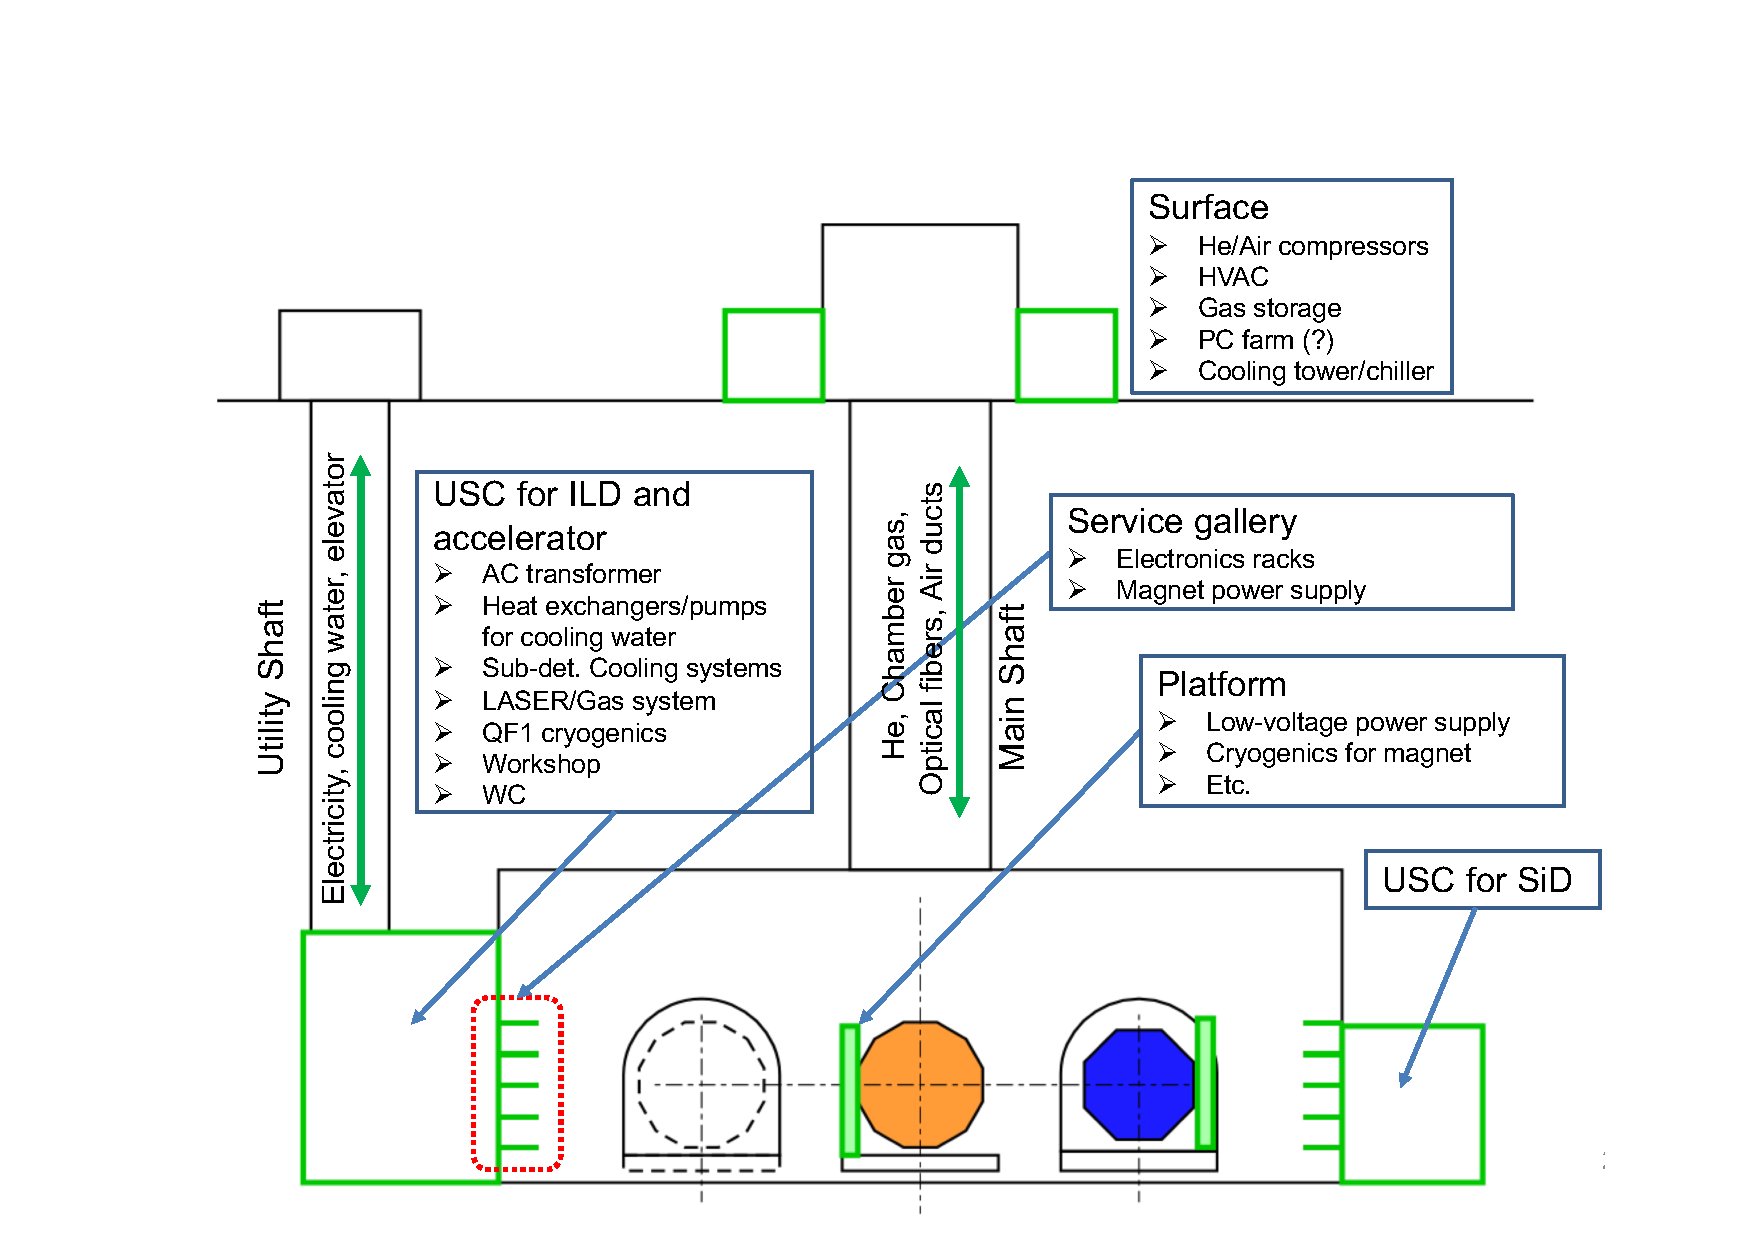
\includegraphics[width=1.0\hsize]{Integration/fig/Services_v2.pdf}
\caption{\label{fig:integration:services}Schematic drawing of the possible locations for detector services. The Utility/Service cavern (USC) for the detector is proposed but not yet implemented into the ILC baseline design~\cite{ild:bib:services_figure}. }
\end{figure}

\begin{figure}[h!]
\centering
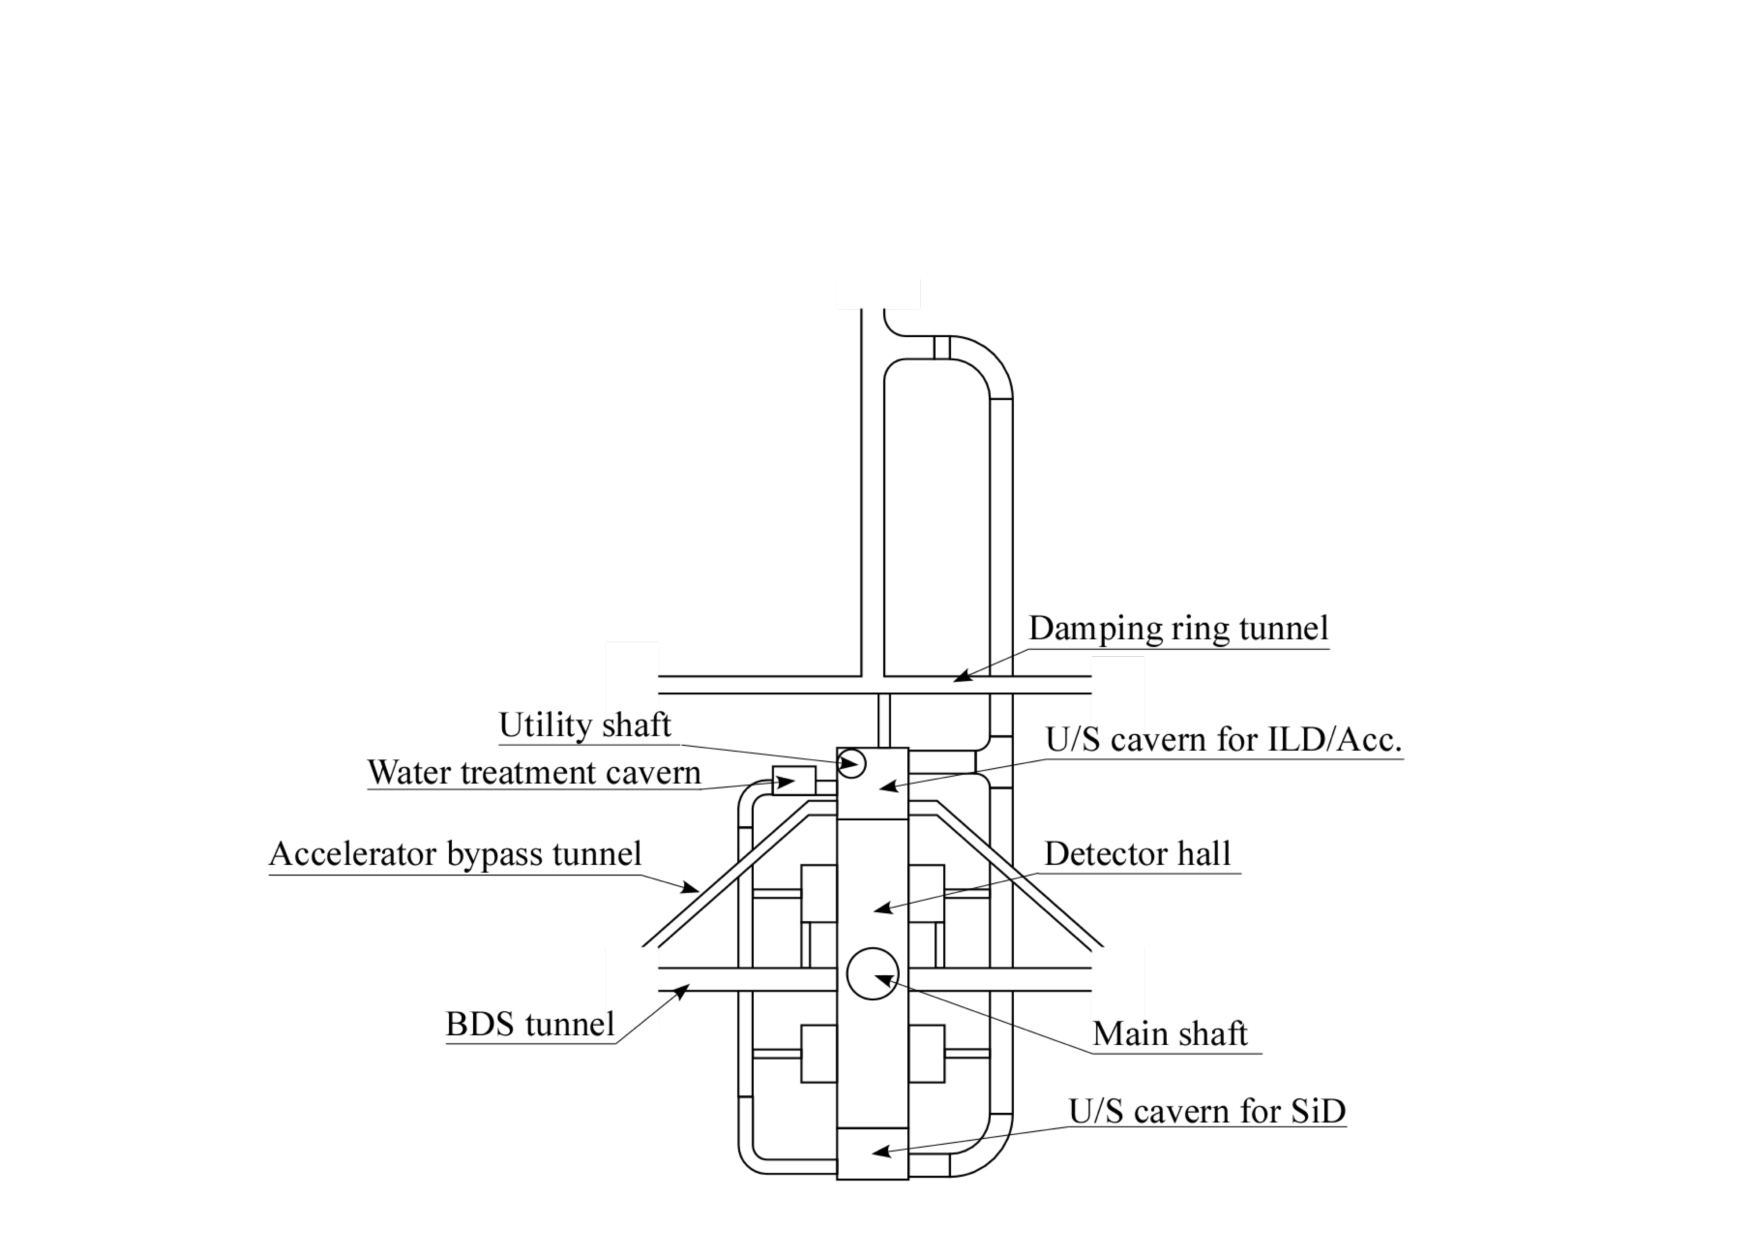
\includegraphics[width=1.0\hsize]{Integration/fig/underground.pdf}
\caption{\label{fig:integration:USC}A possible design of Utility/Service caverns. }
\end{figure}

\subsubsection{Power Consumption and Cooling Requirements}
\label{ild:sec:power}
The requirements for power and cooling at ILD have been studied in a bottom-up approach where the current information from all detector components has been assembled and cross-checked.

A tentative estimation of the power consumption in the detector hall and surface facilities for ILD is listed in Table~\ref{tab:integration:power}. The total power consumption in the underground caverns is about 1~MW, dominated by the ILD solenoid and the machine components associated to the detector. 

The cooling water which is necessary for extracting the power consumption is shown in Table~\ref{tab:integration:cooling}.
Distribution of the underground power is visualized in Figure~\ref{fig:integration:power}. It can be seen that the fraction of the power consumption that is coming from the sub-detectors is small.

\begin{table}[htb]
    \centering
    \begin{tabular}{l|l|c|c|c|c}
       \multicolumn{2}{l|}{{\bf Item}} & {\bf Power} &\multicolumn{3}{c}{ } \\ \hline
        \multirow{3}{*}{QD0/QF1/Crab Cavity} & Power Supply  & 150 & \multicolumn{3}{l}{ } \\
                            & Cold Box      & 150 & \multicolumn{3}{l}{ } \\
                            & He Compressor & 300 & \multicolumn{3}{l}{on surface}\\ \hline
        \multirow{3}{*}{Detector Solenoid} & Power Supply  & 250 & \multicolumn{3}{l}{ } \\
                            & Cold Box      & 50 & \multicolumn{3}{l}{ } \\
                            & He Compressor & 500 & \multicolumn{3}{l}{on surface}\\ \hline                      
        \multirow{10}{*}{Subdetectors} & {\bf Total}  & {\bf 161} & {\bf Front-end Electr.} & {\bf Back-end Electr.} & {\bf Cooling}\\ \cline{2-6}
        & Muon  & 12 & 5 & 5  & 2 \\
        & HCAL  & 45.5 & 27.5 & 8 & 10 \\
        & ECAL  & 40 & 20 & 12 & 8 \\
        & VFS   & 9 & 2 & 5 & 2 \\
        & SET   & 9 & 2 & 5 & 2 \\
        & TPC   & 16.2 & 15 & - & 1.2 \\
        & SIT   & 8 & 1 & 5 & 2 \\
        & FTD   & 8 & 1 & 5 & 2 \\
        & VTX   & 13.5 & 2 & 1.5 & 10 \\\hline
        \multicolumn{2}{l|}{Computer Farm}& 1000 & \multicolumn{3}{l}{on surface}\\ \hline
        \multicolumn{2}{l|}{Water Pump}& 25 & \multicolumn{3}{l}{}\\ \hline
        \multicolumn{2}{l|}{HVAC}& 600 & \multicolumn{3}{l}{on surface}\\ \hline
        \multicolumn{2}{l|}{Lighting}& 25 & \multicolumn{3}{l}{}\\ \hline
        \multicolumn{2}{l|}{Air Compressor}& 50 & \multicolumn{3}{l}{on surface}\\ \hline
        \multicolumn{2}{l|}{Platform Mover}& 100 & \multicolumn{3}{l}{}\\ \hline
        \multirow{2}{*}{Cranes} & 3x5t & 21 & \multicolumn{3}{l}{}\\
        & 40t & 50 & \multicolumn{3}{l}{}\\ \hline
        \multicolumn{2}{l|}{{\bf TOTAL}}& {\bf 3432} & \multicolumn{3}{l}{}\\ \hline
        \multicolumn{2}{l|}{Underground}& 982 & \multicolumn{3}{l}{}\\ \hline
    \end{tabular}
    \caption{Breakdown of the power consumption estimates for the ILD detector and appended ILC components (in kW)~\cite{ild:bib:services}. Power-pulsing operations are assumed for the ILD subdetectors.}
    \label{tab:integration:power}
\end{table}

\begin{table}[]
    \centering
    \begin{tabular}{m{1.4cm}|m{1.7cm}|m{0.6cm}|m{0.6cm}|m{0.7cm}|m{0.6cm}|m{0.6cm}|m{0.7cm}|m{0.6cm}|m{0.6cm}|m{0.7cm}}
    \multicolumn{2}{m{1.4cm}|}{}& \multicolumn{3}{c|}{Chilled Water} & \multicolumn{3}{c|}{Low-conductive Water} & \multicolumn{3}{c}{Normal Water} \\ \hline
    \multicolumn{2}{m{1.4cm}|}{Item} & Heat (kW) & $\Delta$T (K) & Flow (l/min) & Heat (kW) & $\Delta$T (K) & Flow (l/min) & Heat (kW) & $\Delta$T (K) &Flow (l/min) \\ \hline
    \multirow{2}{1.4cm}{QD0/QF1/ Crab Cav.} & Power Supply & & & & 150 & 10 & 214 & & & \\
    & Cold Box & & & & 150 & 10 & 214 & & & \\\hline
    \multirow{2}{1.4cm}{Detector Solenoid} & Power Supply & & & & 250 & 10 & 357 & & & \\
    & Cold Box & & & & 50 & 10 & 71 & & & \\\hline
    \multirow{9}{1.4cm}{Subdetectors} & Muon & 12 & 5 & 34 & & & & & \\
    & HCAL & 45.5 & 5 & 130 & & & & & & \\
    & ECAL & 40 & 5 & 114 & & & & & & \\
    & VFS & 9 & 5 & 26 & & & & & & \\
    & SET & 9 & 5 & 26 & & & & & & \\
    & TPC & 3 & 5 & 5 & & & & 13 & 5 & 38\\
    & SIT & 8 & 5 & 23 & & & & & & \\
    & FTD & 8 & 5 & 23 & & & & & & \\
    & VTX & 13.5 & 5 & 39 & & & & & & \\\hline
    \multicolumn{2}{m{2cm}|}{Pump} & 11 & 5 & 31 & 11 & 10 & 16 & 3.7 & 5 & 11\\ \hline
    \multicolumn{2}{m{2cm}|}{AC Transformer} & 49 & 5 & 140 & & & & & & \\ \hline
    \multicolumn{2}{m{2cm}|}{{\bf Total}} & 208 & & 595 & 611 & & 873 & 17 & & 48 \\ \hline
    \multicolumn{2}{l|}{{\bf Total Chilled Water}} & \multicolumn{3}{r|}{{\bf 595}} & \multicolumn{6}{r}{}\\ \hline
    \multicolumn{2}{l|}{{\bf Total Normal Temp. Water}} & \multicolumn{3}{r|}{} & \multicolumn{6}{r}{{\bf 921}}\\ \hline

    \end{tabular}
    \caption{Breakdown of the cooling water requirement estimates for ILD and appended ILC components~\cite{ild:bib:services}.}
    \label{tab:integration:cooling}
\end{table}

\begin{figure}[h!]
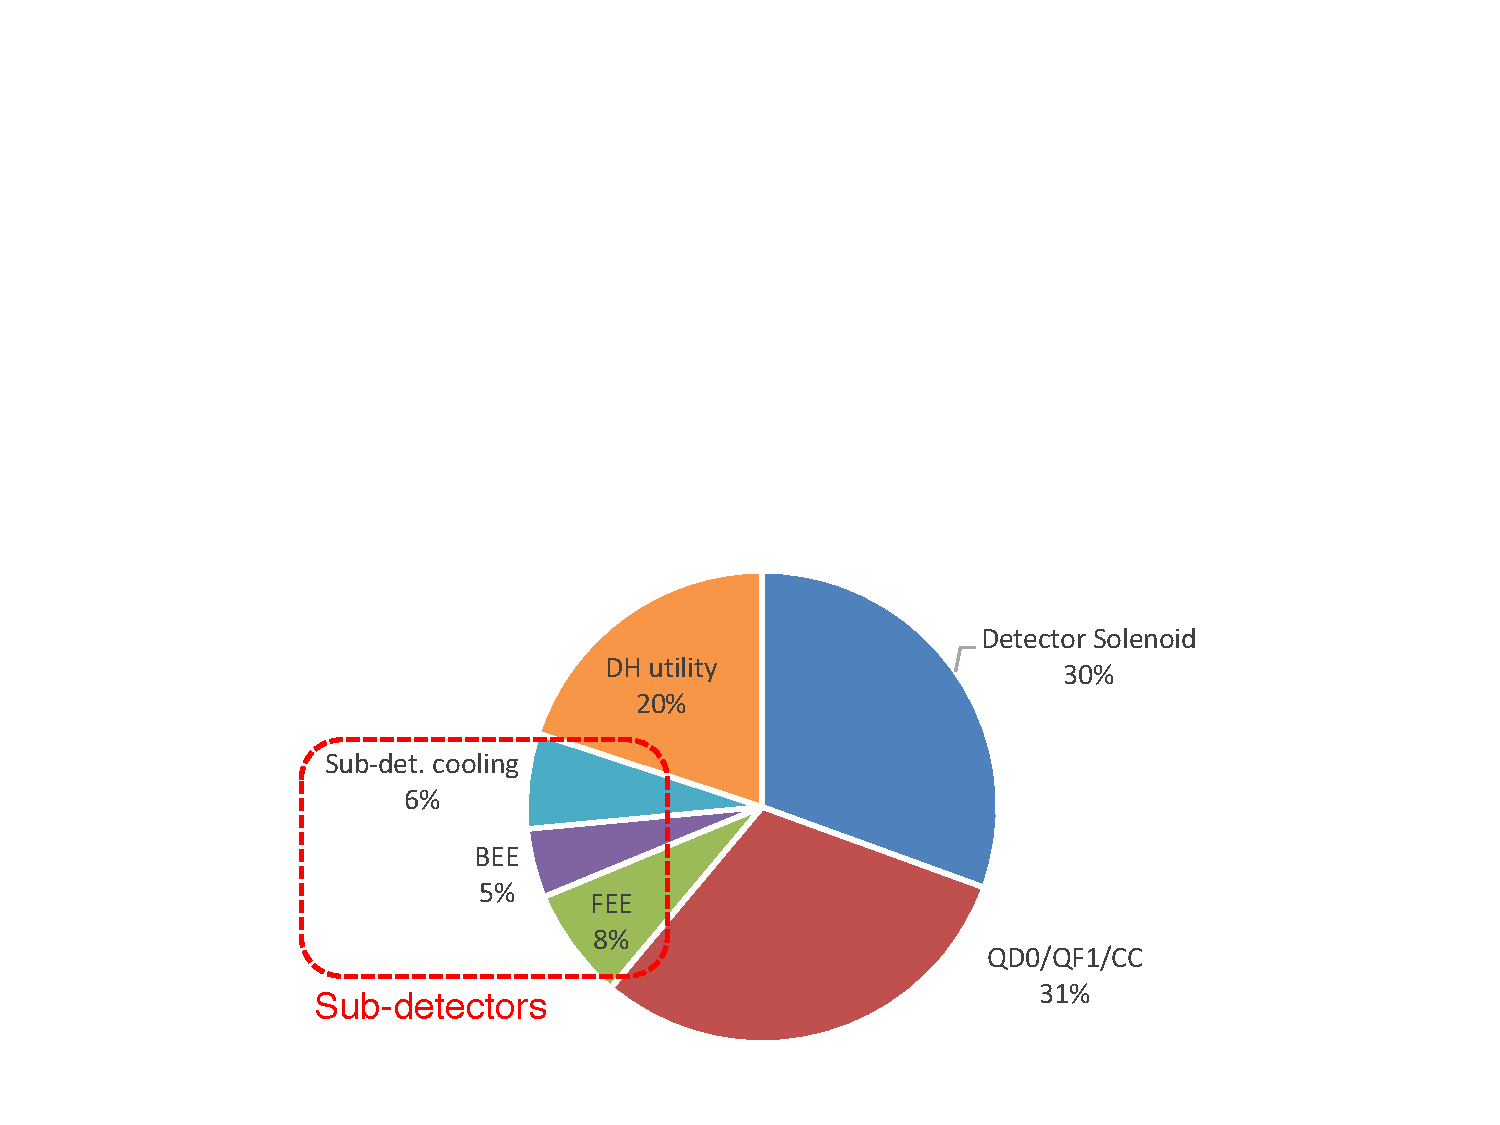
\includegraphics[width=0.7\hsize]{Integration/fig/Power.pdf}
\caption{\label{fig:integration:power}Distribution of the underground power consumption for ILD~\cite{ild:bib:services}. While the detector solenoid, the machine elements (magnets QD0/QF1 and the crab cavity system CC) use the major part of the power, the detector hall (DH) utilities and the sub-detectors cooling, back- and front-end electronics (BEE, FEE) contribute less. The total power consumption sums up to about 1~MW.}
\end{figure}
\vspace{2cm}
\FloatBarrier

\subsection{Access and Assembly}
\label{ild:sec:access}
The Kitakami site of the ILC is located in a mountainous and rural area, only accessible by road~(c.f.~Figure~\ref{ild:fig:ilc_site}). The nearest port, Kesennuma, is about 40~km away on the Pacific coast. All ILD parts need to be shipped via the central access roads into the mountains. Typically, street transport in Japan is limited to trucks with up to 25~t of mass (including the weight of the truck itself). The total mass of ILD is of about 15,500~t, posing a specific challenge for the logistics infrastructure. Heavy-load transports of up to 70~t loads are possible in exceptional cases. For the transport of the ILD solenoid modules, this option is under study~(c.f.~Figure~\ref{ILD:fig:magnet_transport}).

The heaviest parts of ILD are the yoke rings. They need to be assembled on-site from pre-fabricated iron blocks. Figure~\ref{fig:integration:yoke_assembly} shows three options that are under study for the procedures. If a remote campus close to the interaction region could be made available, with a dedicated reinforced street in-between, then the pre-fabricated iron slabs from the factory could be assembled into blocks of up to 200~t there. The blocks could then be transported via the dedicated road to the interaction region for assembly of the yoke rings. Another option would be the construction of a pre-assembly hall at the interaction region. The construction of the iron block could then take place there, in the vicinity of the detector assembly hall and therefore a reduced transportation problem. A remote area would still be useful as storage space. 

%The exact configuration of a possible remote %campus and the IP campus depends on local %boundary conditions and also has an impact on %the project cost and is therefore subject to %future optimisation studies.

\begin{figure}[h!]
\centering
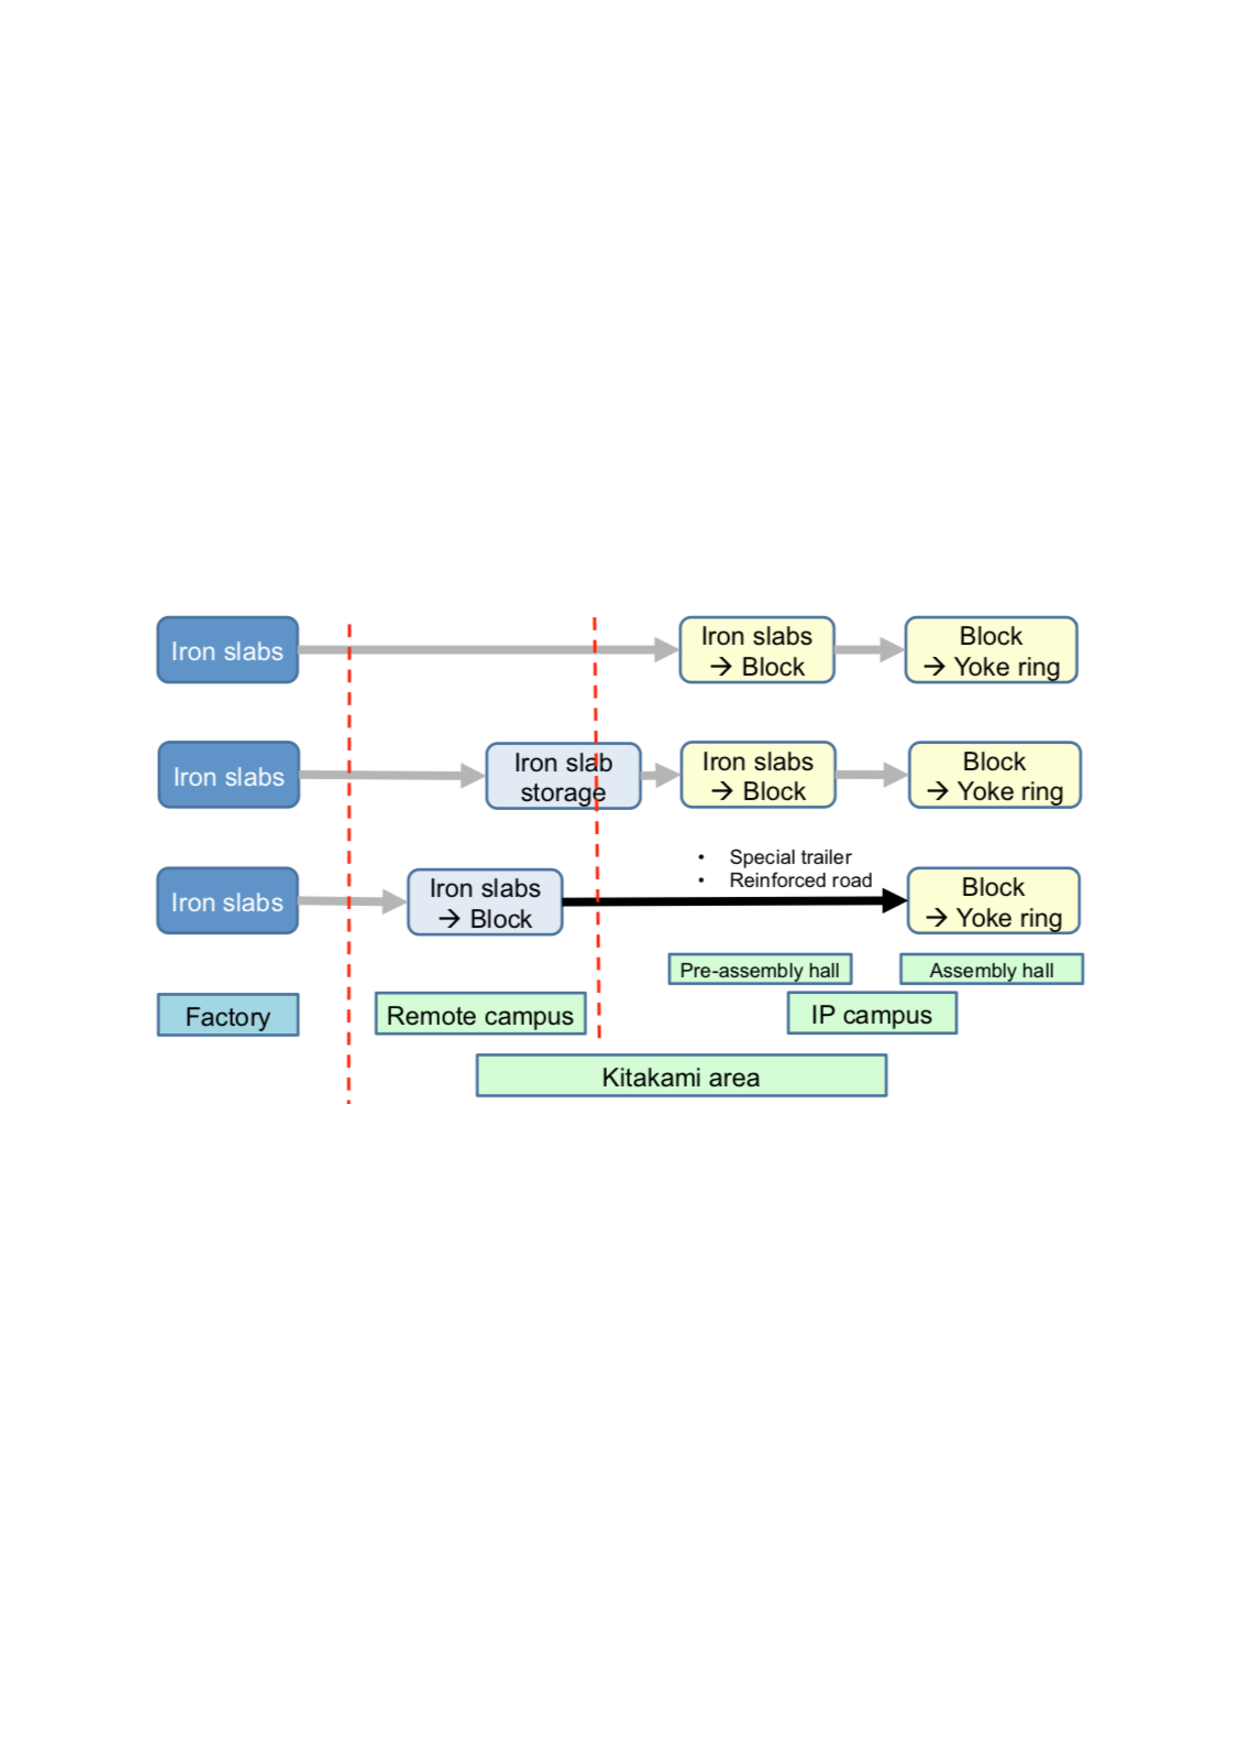
\includegraphics[width=0.8\hsize]{Integration/fig/yoke_assembly.pdf}
\caption{\label{fig:integration:yoke_assembly}Options under study for the (pre)assembly of the ILD iron return yoke~\cite{ild:bib:ejade_mdi}.}
\end{figure}

Figure~\ref{fig:integration:surface} shows a conceptual layout of the surface installations above the interaction region. The central detector assembly hall serves both detectors, SiD and ILD, and is located above the central access shaft to the underground areas (compare Figure~\ref{fig:integration:underground}). A pre-assembly building for SiD and ILD is located right next to it. Heavy and large parts, like the ILD yoke blocks, could be assembled in the pre-assembly area before they are moved to the central assembly hall for the installation of the yoke rings.
%\begin{figure}[p]
%\centering
%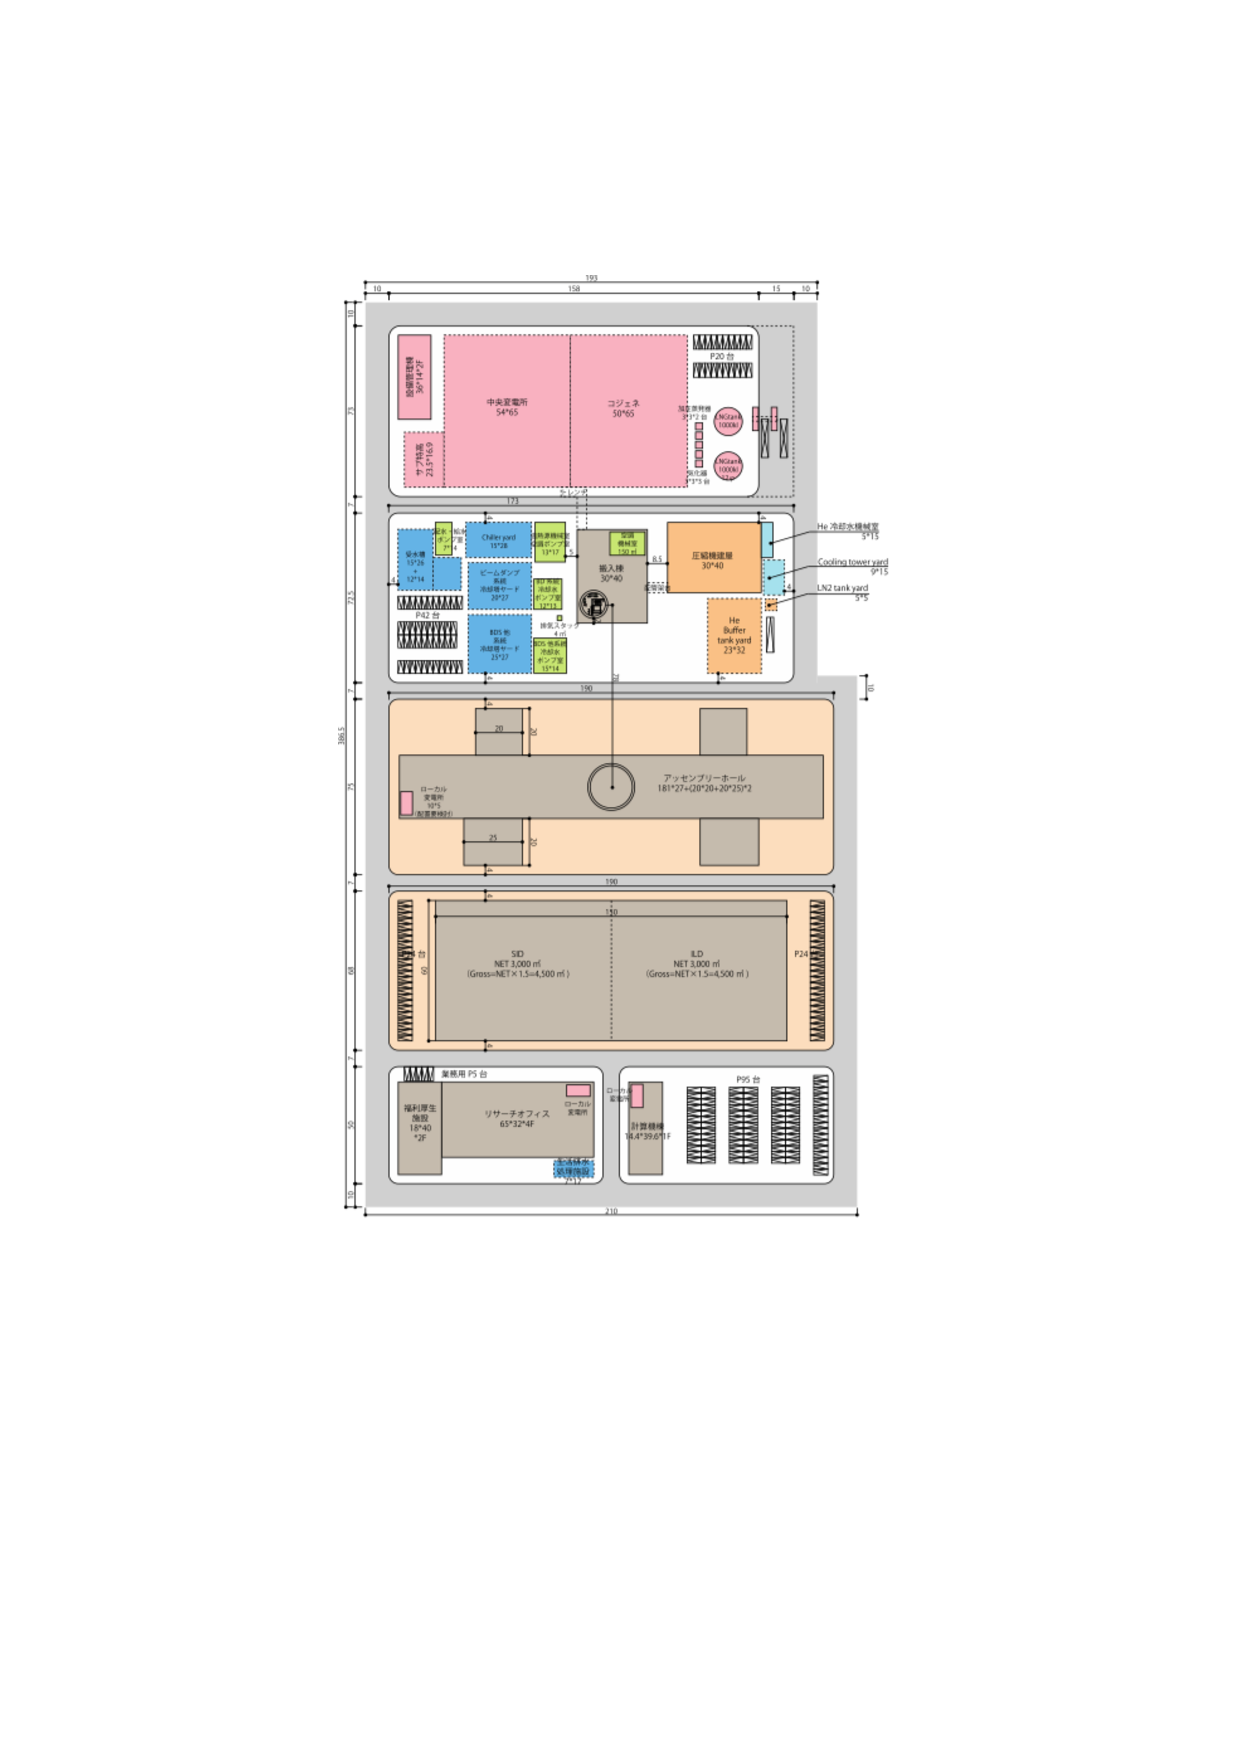
\includegraphics[width=0.8\hsize]{Integration/fig/interaction_area.pdf}
%\caption{\label{fig:integration:interaction_area}Conceptual design of the %interaction area surface installations with the detector assembly hall over %the large shaft in the middle and with a dedicated detector pre-assembly %building next to it~\cite{ild:bib:ejade_mdi}.}
%\end{figure}

A survey has been done within ILD to assemble the requirements of the sub-detectors on assembly, storage and on-site testing space. Figure~\ref{fig:integration:assembly_space} shows the results from SDHCAL, TPC and SiECAL (barrel and endcap). Though the information is at a very conceptual level, it serves as valuable input for the planners of the interaction region surface installations that need to be accommodated in the Kitakami mountains. 

The distribution of work between main campus, a possible remote campus, and the IP campus depends on the exact availability and possible locations and needs to be worked out in detail, once the boundary conditions are better known.

It should be noted, that the assembly of the detector takes only a limited amount of time and that some of the foreseen buildings, as the detector preparation building, could be made from temporary structures so that part of the occupied area could be recultivated again.

\begin{figure}[h!]
\centering
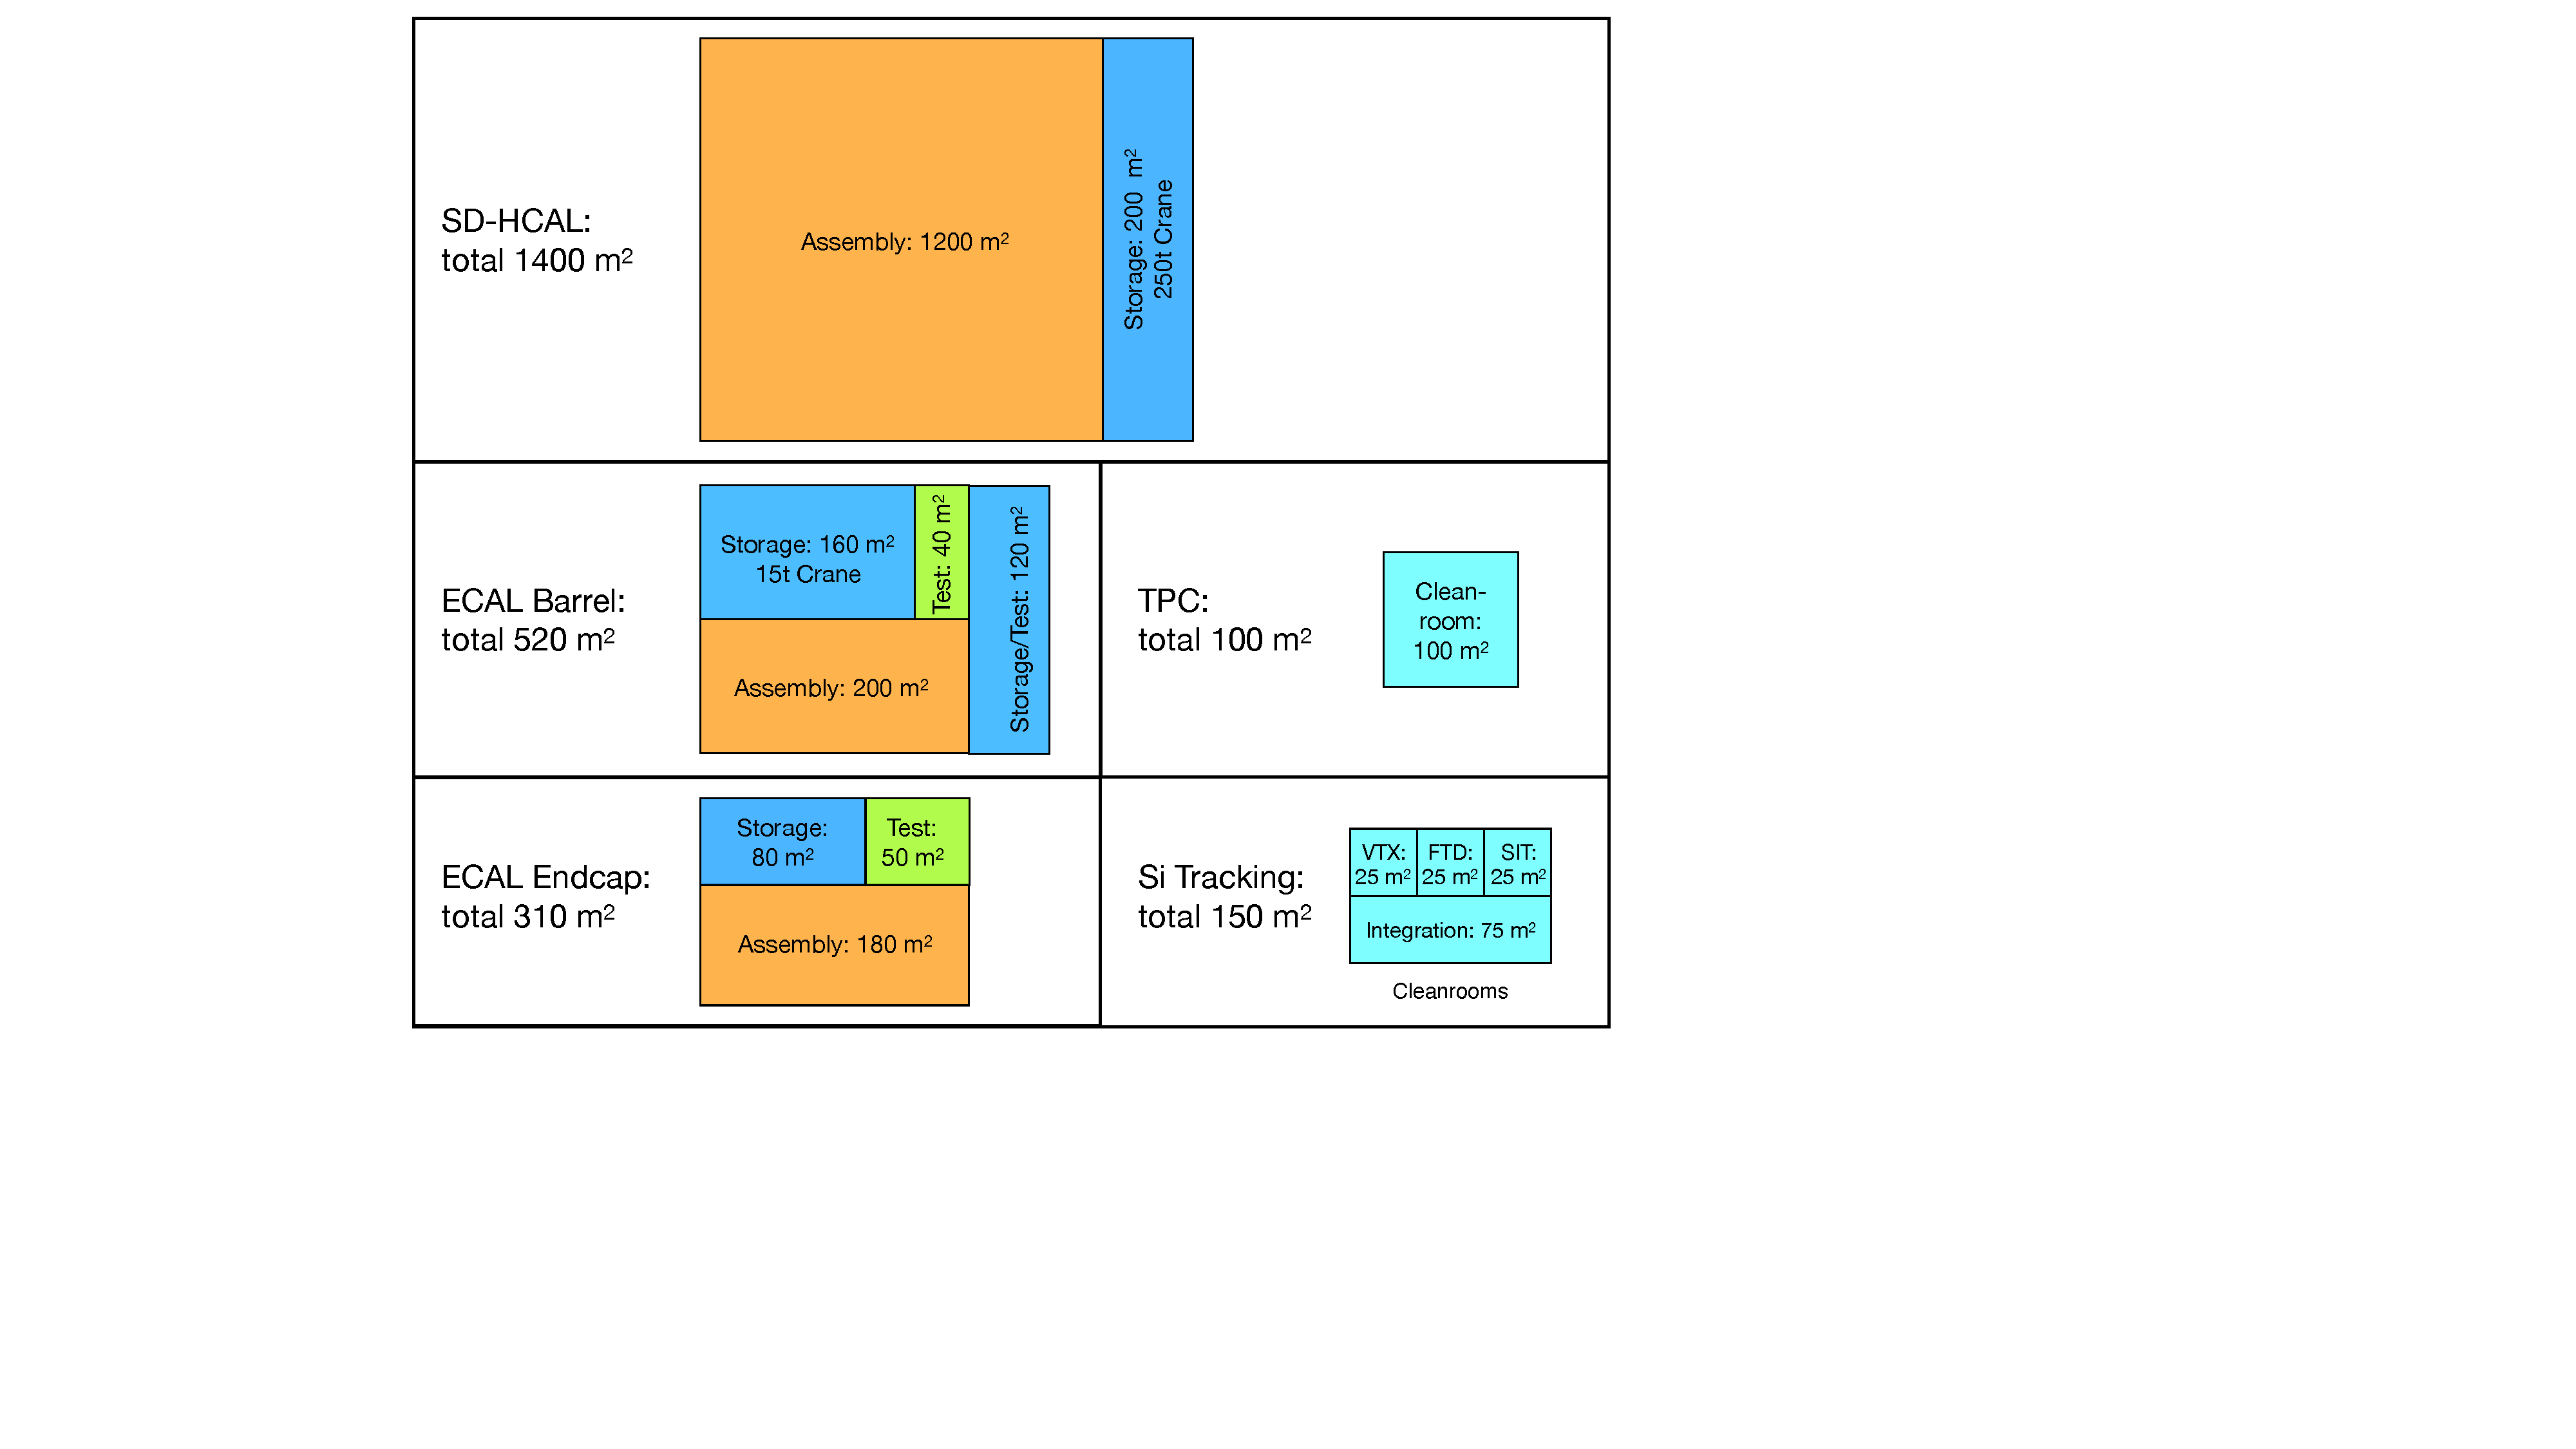
\includegraphics[width=0.8\hsize]{Integration/fig/Assembly_Space.pdf}
\caption{\label{fig:integration:assembly_space}Result of a subdetector survey on assembly space requirements~\cite{ild:bib:ejade_mdi,ild:bib:assembly}.}
\end{figure}

The final assembly of ILD and SiD should happen above ground in the central detector assembly hall. The major parts, the SiD barrel detector and the ILD yoke rings, have masses of up to 4500~t and will be lowered through the central access shaft into the underground areas with the help of a gantry crane. A similar procedure has been followed for the CMS detector at CERN and was proven to be very efficient. Figure~\ref{fig:integration:gantry_crane} shows an artists view of the SiD barrel detector hanging from a gantry crane.
\begin{figure}[h!]
\centering
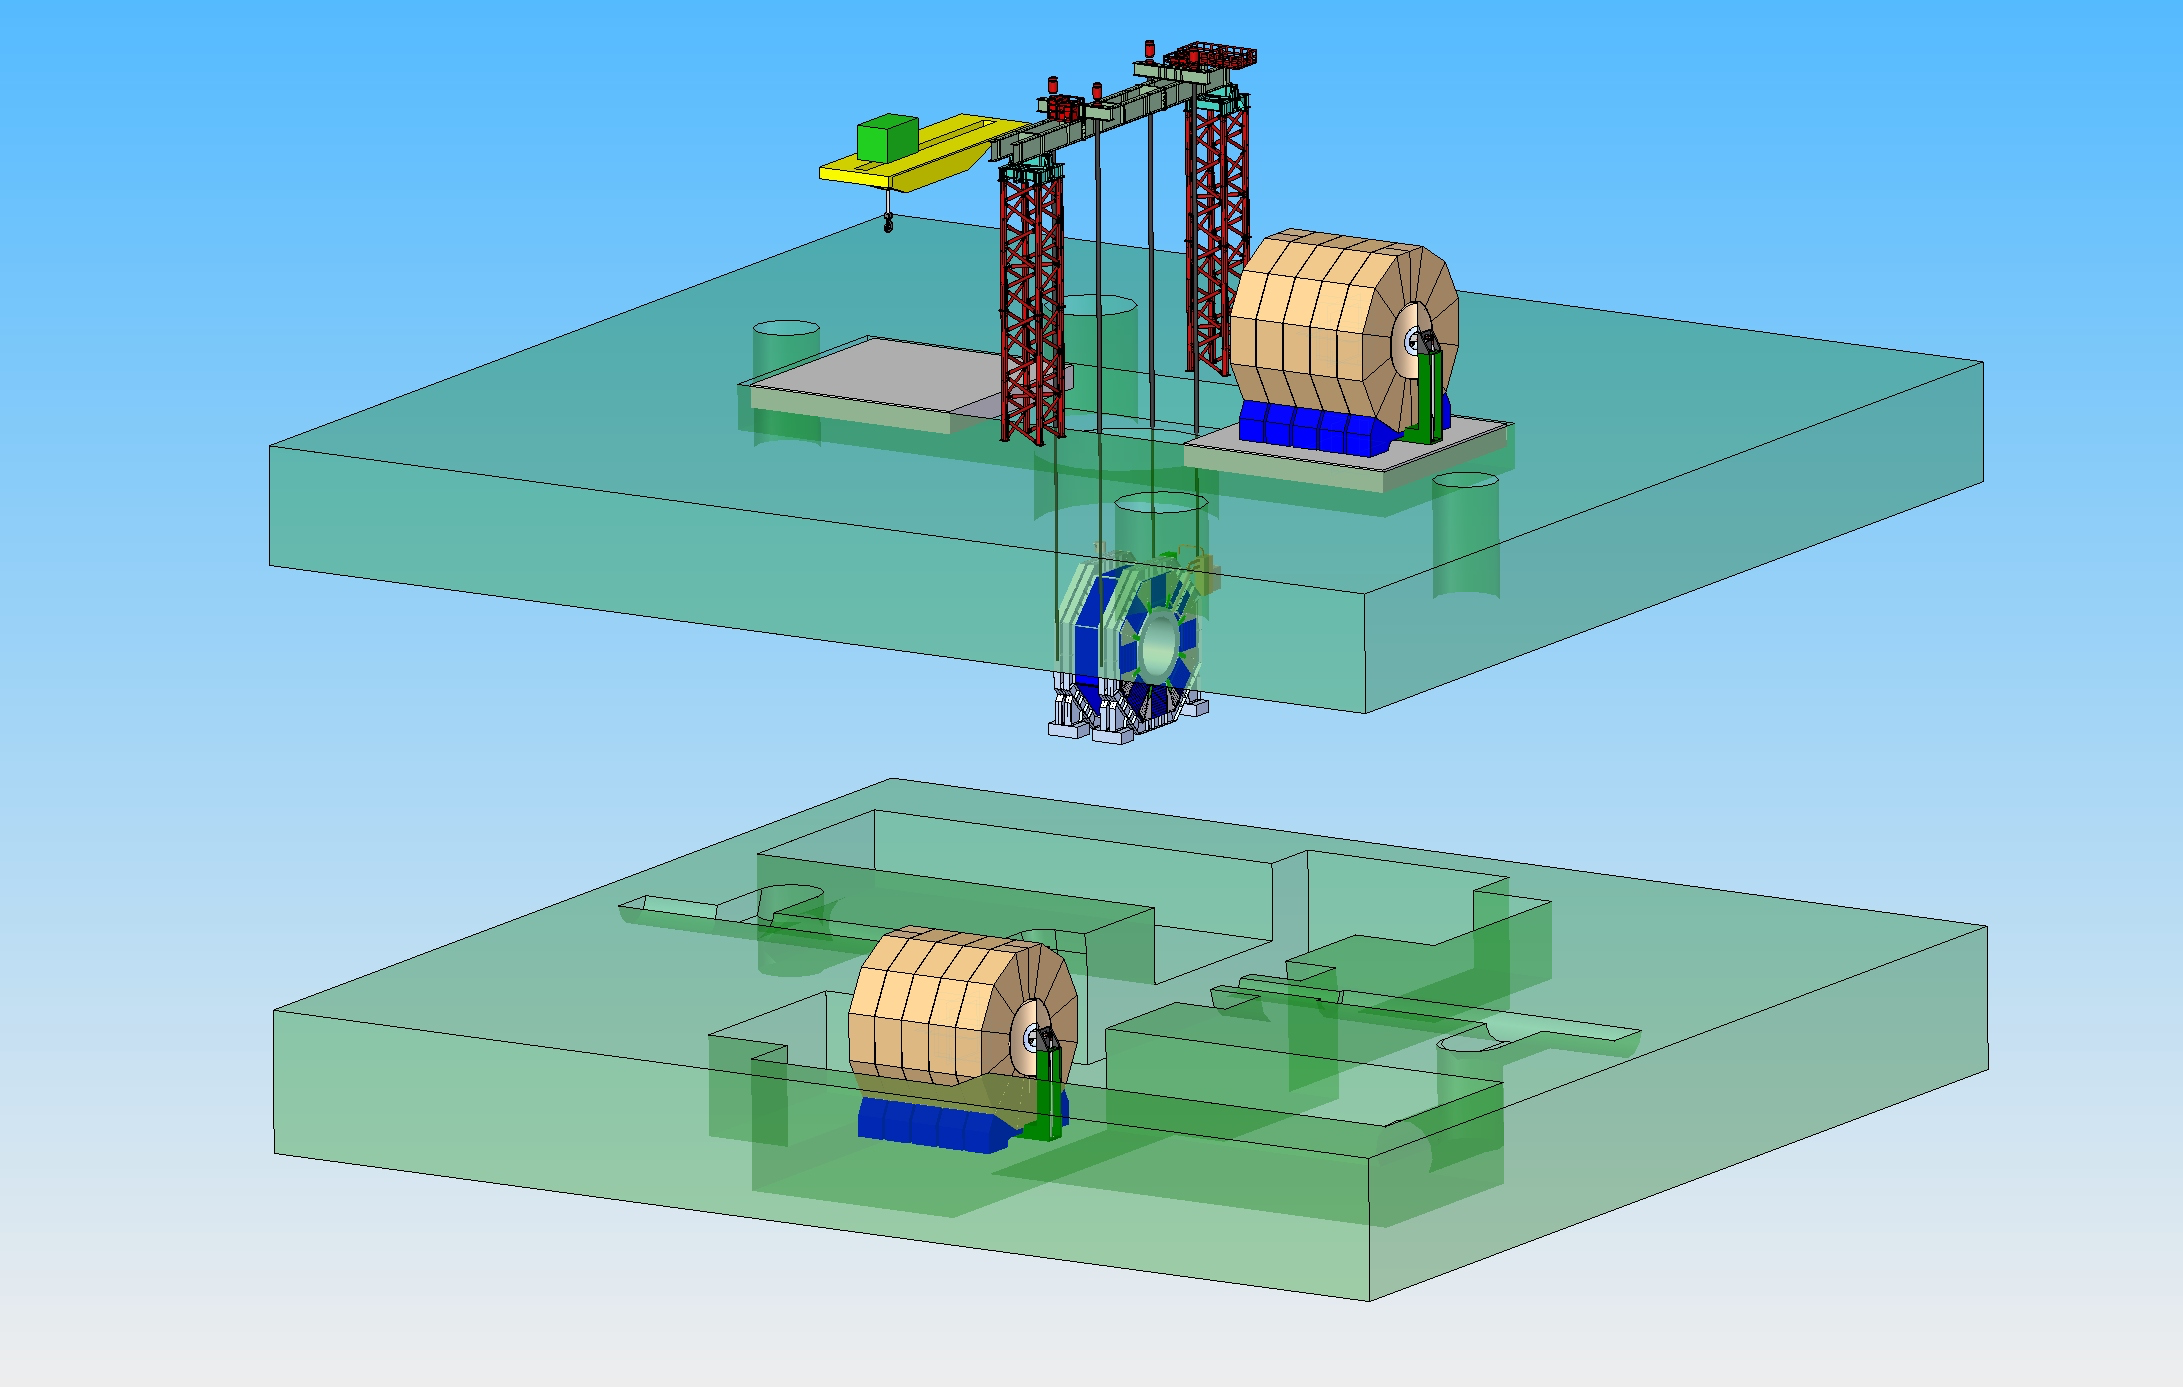
\includegraphics[width=0.8\hsize]{Integration/fig/gantry_crane.png}
\caption{\label{fig:integration:gantry_crane}Lowering of SiD and ILD main parts via the central shaft into the underground detector hall with the help of a heavy load gantry crane~\cite{ild:bib:gantry_crane}.}
\end{figure}

The main advantage of the CMS-style surface assembly of the detectors lies in the decoupled time lines for the construction of the machine and the detectors. In this case, the on-site assembly can start as soon as the surface buildings are ready while the underground excavations and constructions can carry on. Figure~\ref{fig:integration:assembly_timeline} shows a rough schedule for the detector construction.
\begin{figure}[h!]
\centering
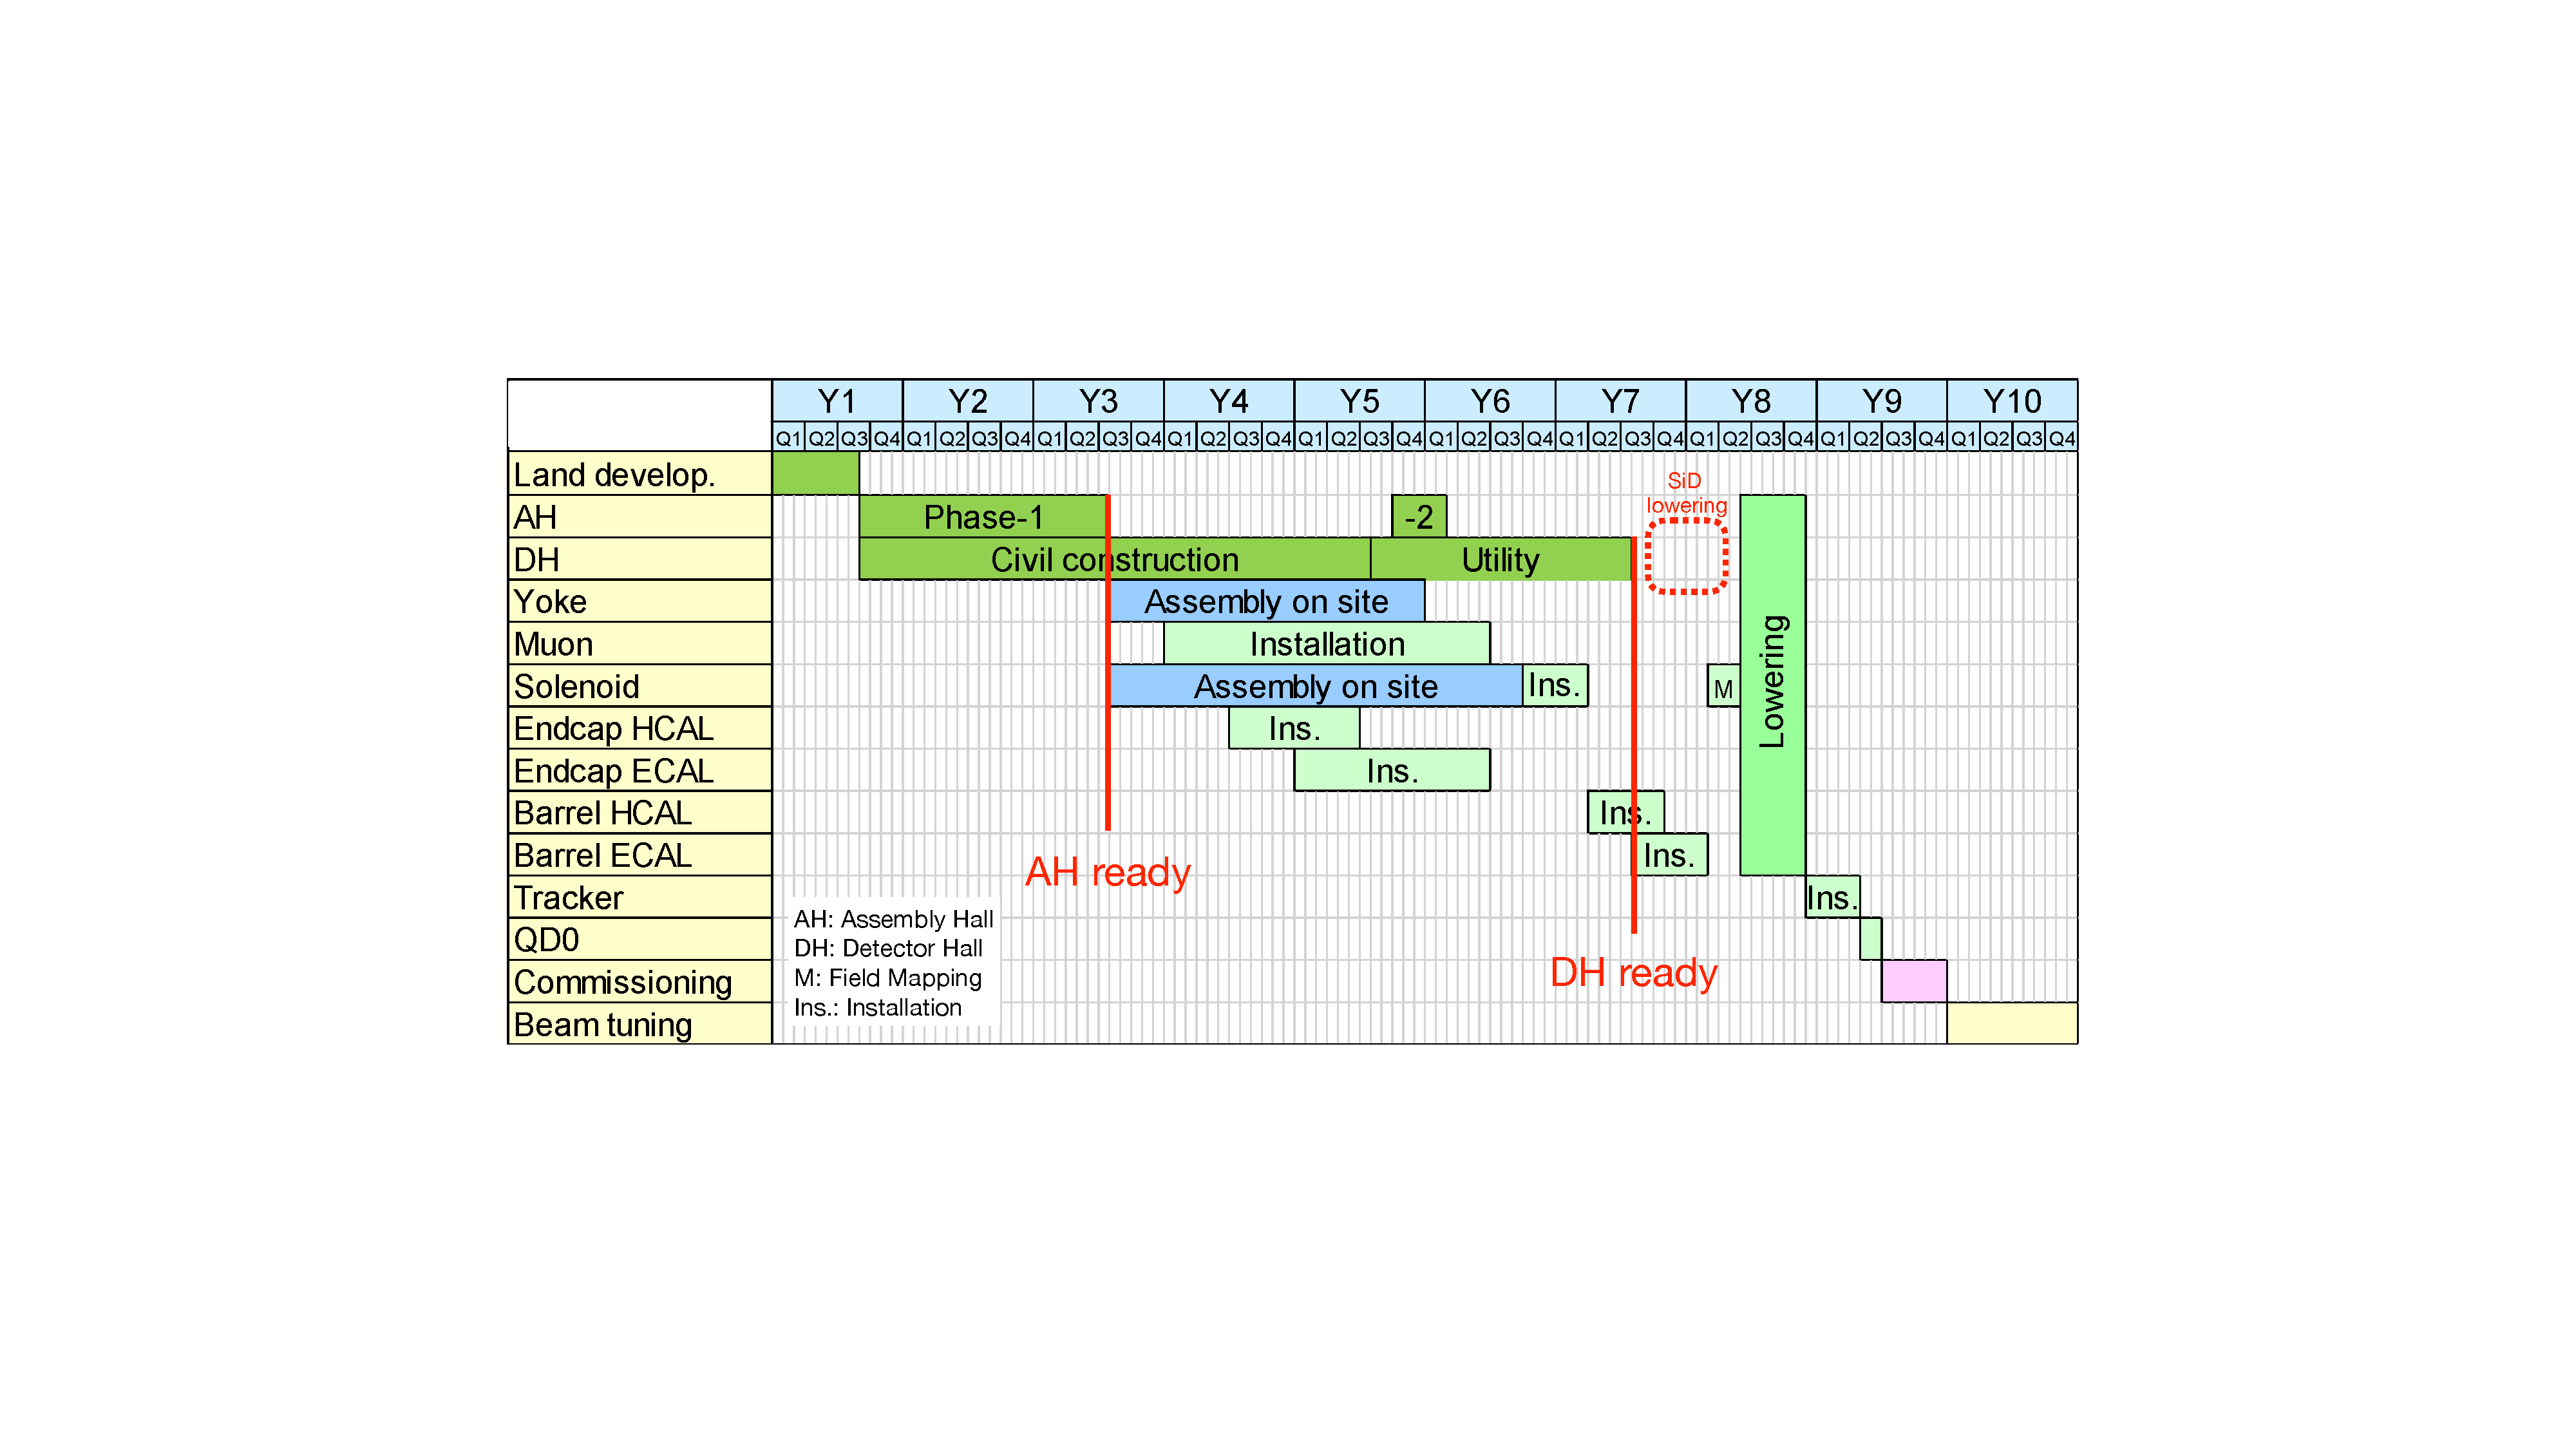
\includegraphics[width=0.8\hsize]{Integration/fig/Detector_Assembly_Timeline.pdf}
\caption{\label{fig:integration:assembly_timeline}Tentative timeline for the detector construction and assembly~\cite{ild:bib:ejade_mdi, ild:bib:assembly}}
\end{figure}
On-site assembly can start 2.5~y after the ground breaking when the surface buildings are ready. The lowering of the large detector parts only takes place about one year before the commissioning of the machine would start. The total technical construction and assembly time is of about 9 years.
\section{Internal ILD integration}
%\writer{Karsten Buesser, Roman Poeschl, Toshiaki Tauchi}{3}

The ILD detector concept underwent a dedicated effort to come to an integrated design that from subdetector level up to the major structures gives a conceptual engineering view of the full system. This includes realistic mechanical designs with tolerances, deformations and dead material zones as well as an integrated design of all detector services: electrical, cooling, gases, etc.

\subsection{ILD Mechanical Structure}

The mechanical structure of ILD has not changed since the DBD~\cite{ild:bib:ilddbd}. The main parts are the three barrel yoke rings and the two endcaps. The central barrel ring carries the solenoid coil in its cryostat; all barrel detectors are suspended from the cryostat. The two other central yoke rings can move over the cryostat. The endcaps can be opened as well. All rings can be moved using airpad systems. Figure~\ref{ILD:fig:mechanical_model} shows the mechanical model of the ILD yoke structure.
\begin{figure}[h!]
    \centering
    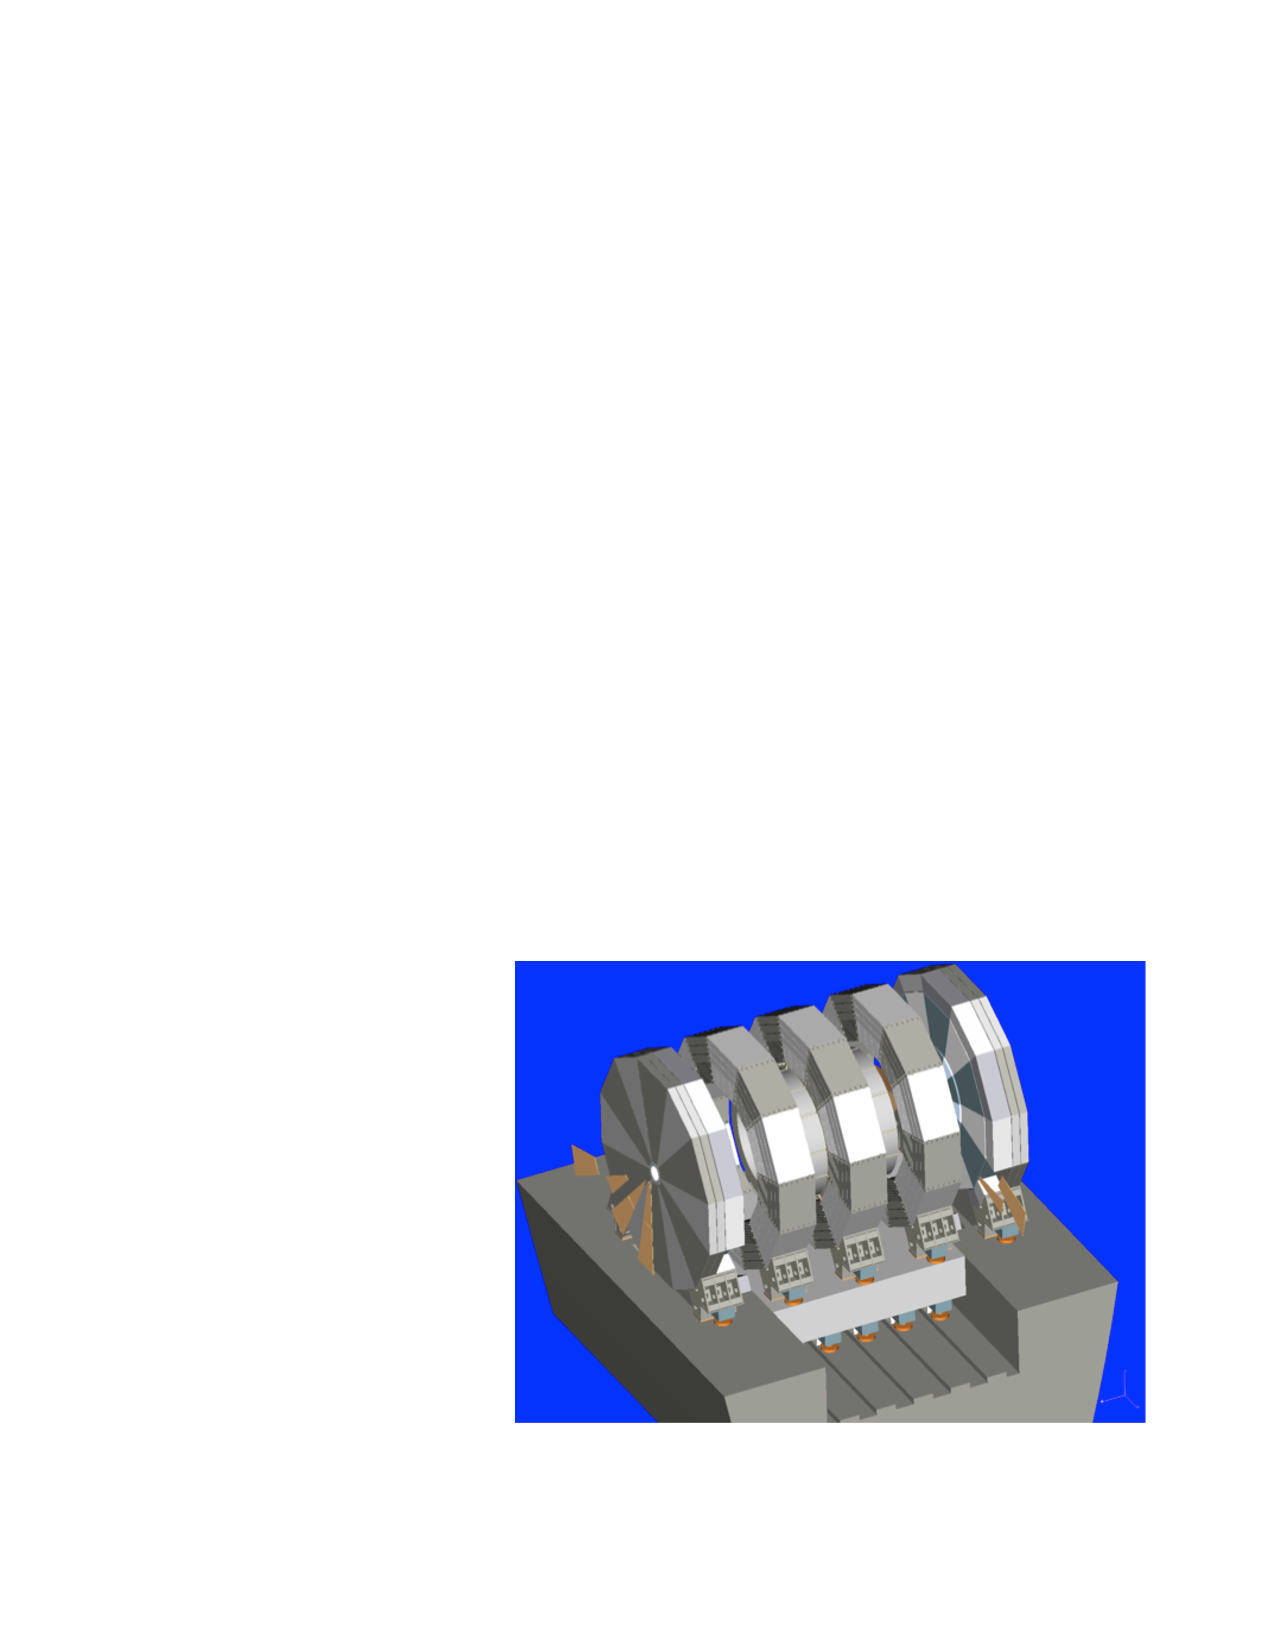
\includegraphics[width=1.0\hsize]{Integration/fig/ILD_Mechanical.pdf}
    \caption{Mechanical structure of the ILD detector~\cite{ild:bib:ilddbd}.}
    \label{ILD:fig:mechanical_model}
\end{figure}


\subsection{ILD Services and Utilities}
\label{ild:sec:services}
Each component of ILD has requirements on services and utilities that are needed for operations and maintenance. This typically includes power and data lines, gas and cooling systems, guidances for laser beams, etc. All major support systems for those services, e.g. power supplies, cooling plants, lasers, DAQ computers, or gas systems are located outside of the detector, sometimes even far away (c.f.~section~\ref{ild:sec:service_locations}). General paths have been defined in the global detector structure where space is allocated for those services. The routing of those paths has to be designed to minimise the amount of gaps and dead material in the active detector areas, while at the same time provide enough space for the foreseen utilities. Three main pathways have been defined for ILD:
\begin{enumerate}
    \item The services of all barrel detectors are collected at both front-faces of the barrel, go around the solenoid cryostat and leave the detector through the gap between the central yoke ring and the neighbouring rings.
    \item The services of the endcap detectors (ECAL, HCAL, Muon) leave the detector along the endcap yoke ring.
    \item The services for the forward calorimeter systems (FCAL, ECAL ring) pass parallel to the beamline, outside of the QD0 magnet.
\end{enumerate}

This scheme allows for the opening of the yoke endcaps as well as for moving the barrel yoke rings independently from each other. The front-end electronic systems of the subdetectors can often drive only a limited cable length. Therefore, space for additional patch panels, drivers, data concentrators needs to be provided inside the ILD detector. While the exact requirements for those are not known in each case, conceptual locations have been defined. Figure~\ref{ILD:fig:cable_paths} shows the general service paths and proposed locations for the patch panels in ILD.

\begin{figure}[h!]
    \centering
    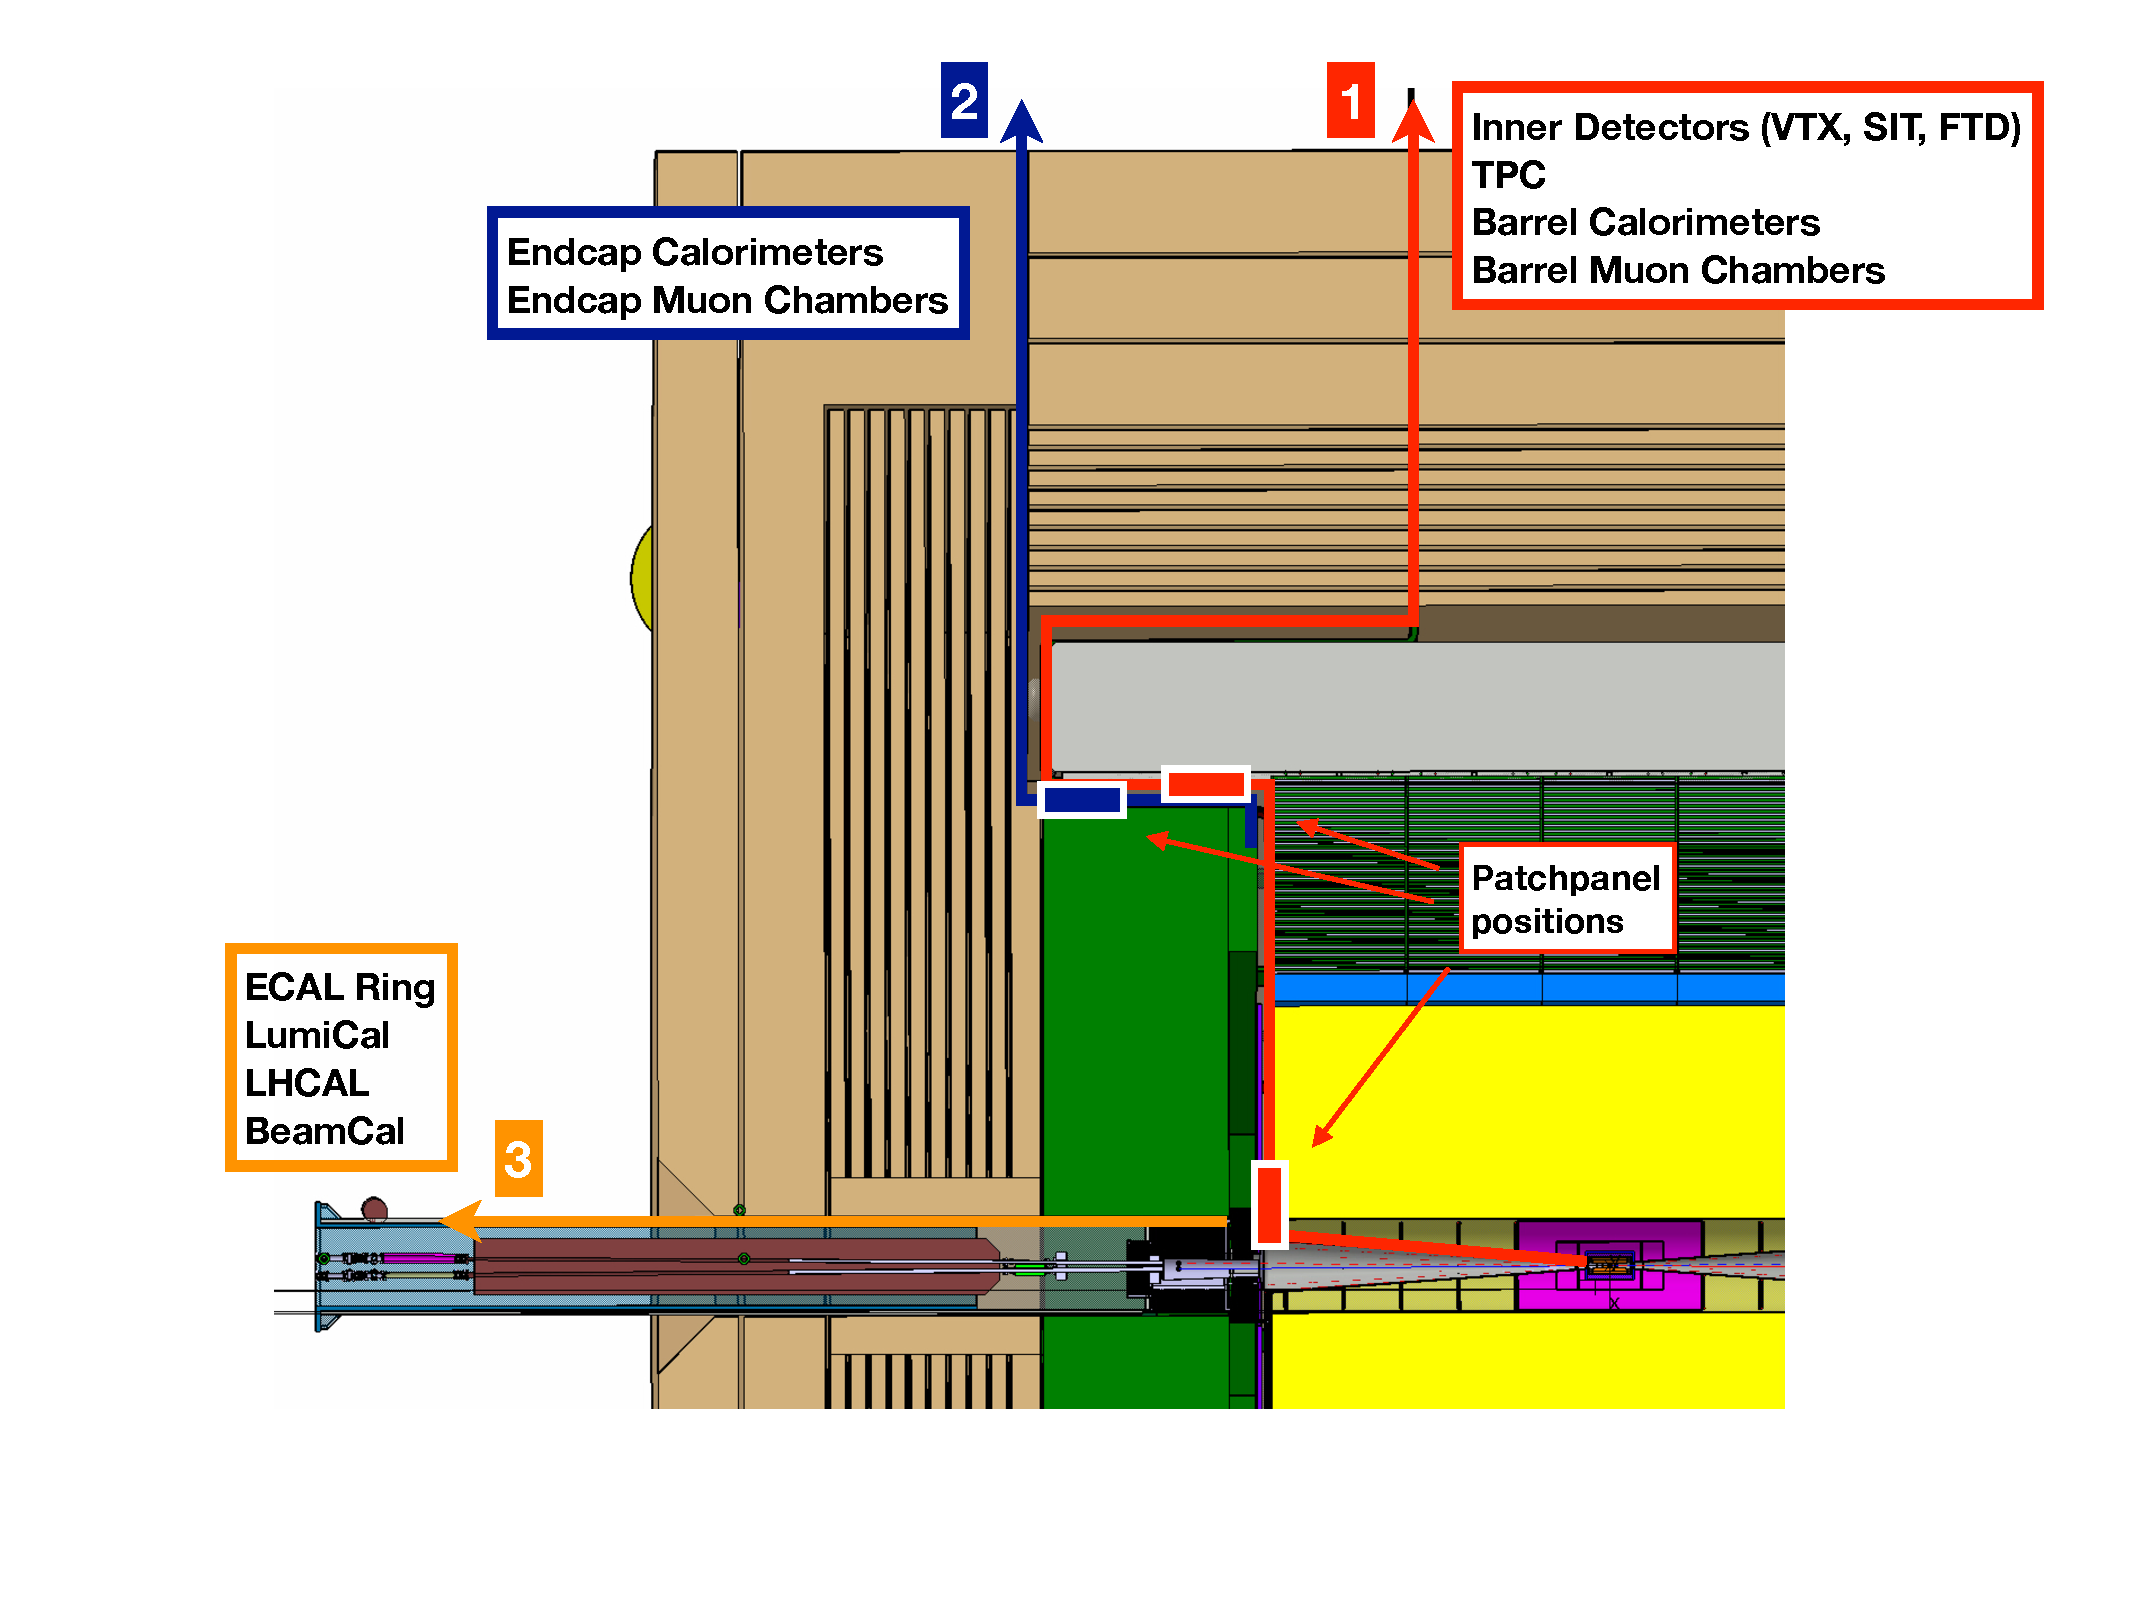
\includegraphics[width=1.0\hsize]{Integration/fig/cable_paths_new.pdf}
    \caption{Service paths in the ILD detector and suggested positions for patch panels.}
    \label{ILD:fig:cable_paths}
\end{figure}


\subsection{Inner Detector Integration}

At the heart of ILD, directly at the interaction point, is the inner detector that comprises the beam pipe as well as the vertex detector and the inner silicon tracking devices, SIT and FTD~(c.f.~Figure~\ref{ILD:fig:inner_detector_schematic}).

\subsubsection{Mechanical Integration}
The vertex detector is suspended from the beam pipe that itself is carried together with the Forward Tracking Disks and the Si Intermediate Tracker from the Inner Detector Support Structure (ISS). The ISS is a support tube made out of carbon-fibre reinforced plastic and is suspended from the end flanges of the TPC. A piezo-based active alignment system (see Figure~\ref{ILD:fig:inner_detector_integration}) allows for the positioning of the ISS with a precision better than 0.01~mm~\cite{ild:bib:inner_detector_integration}, independently of the main ILD detector structure. This is required to adjust the beam pipe and the inner tracking devices with respect to the beam axis, to better precision than what can be achieved with the complete ILD detector, e.g.~after push-pull operations.

\begin{figure}[h!]
    \centering
        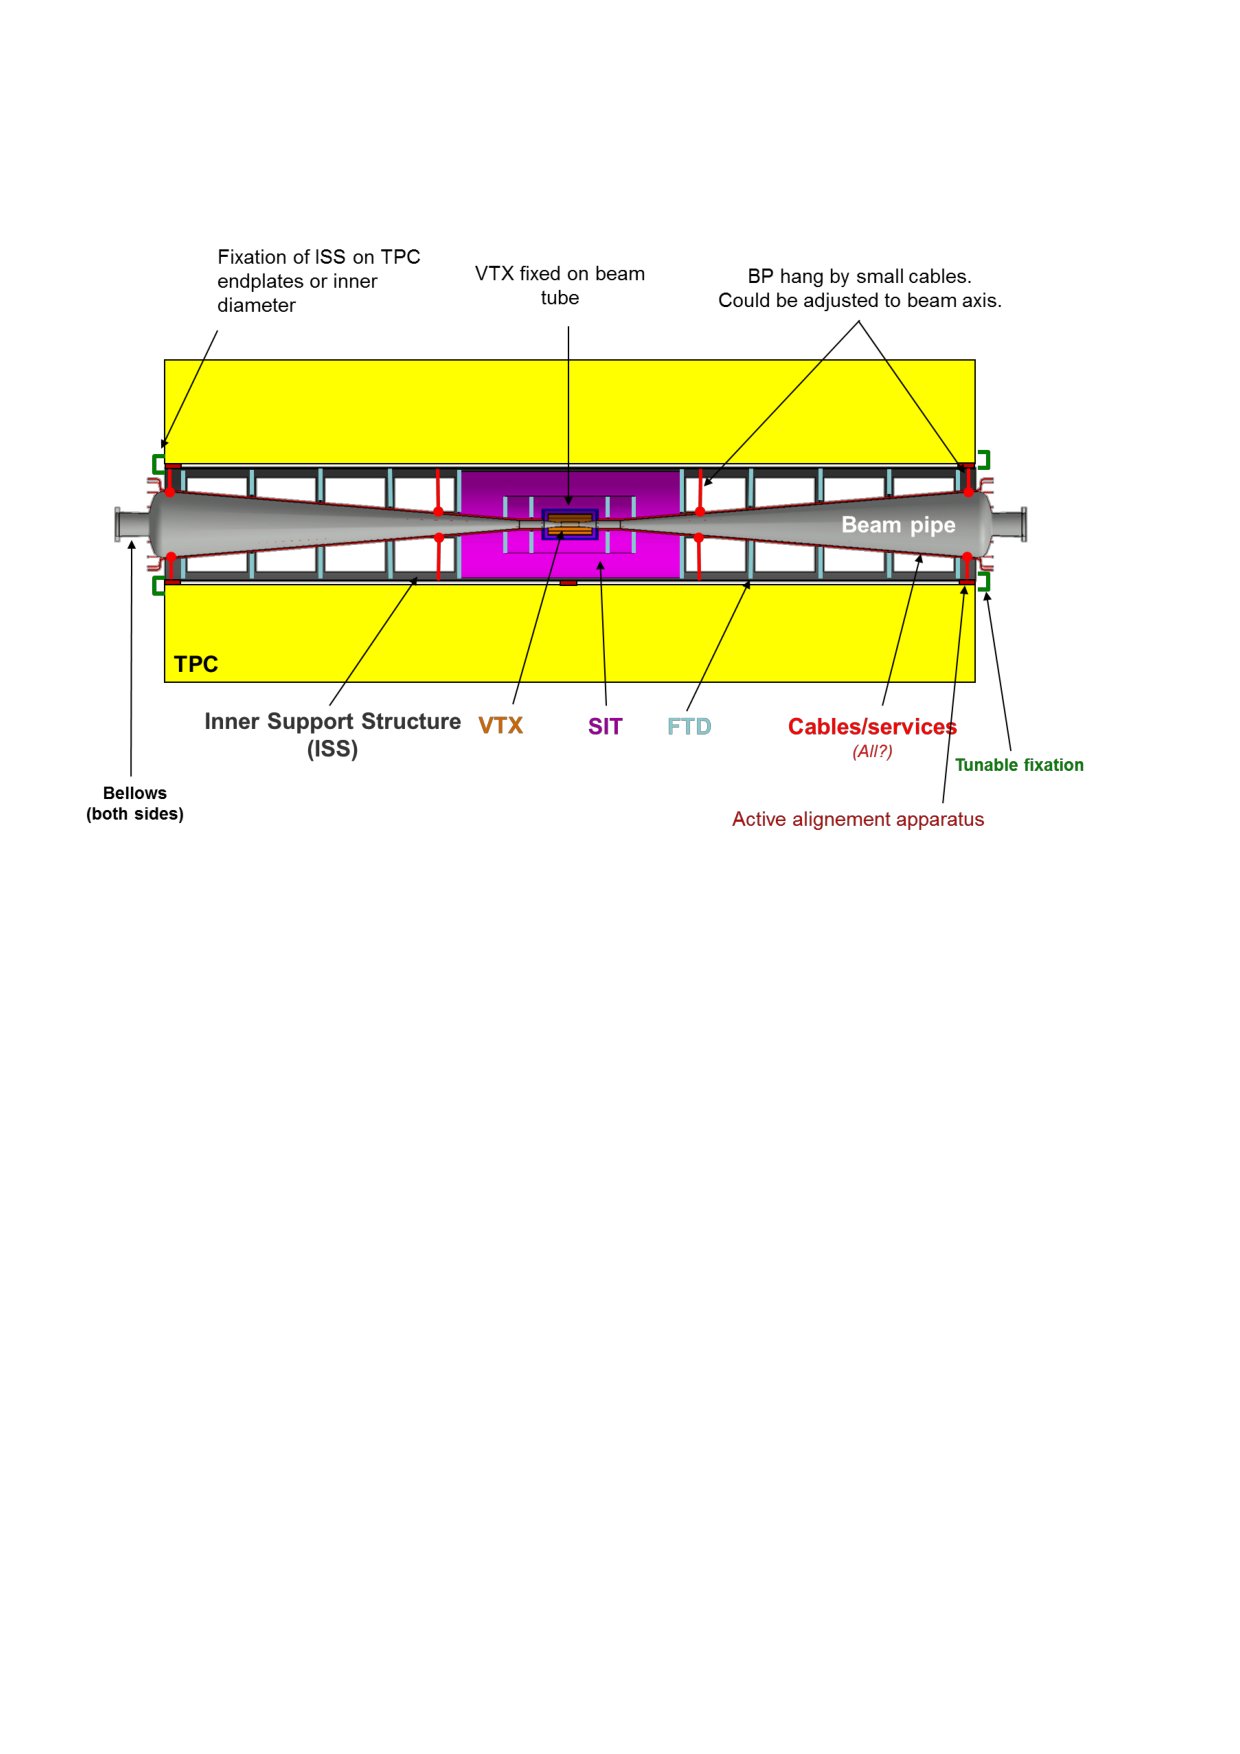
\includegraphics[width=0.8\hsize]{Integration/fig/Inner_Detector_Schematic.pdf}
    \caption{Schematic of the inner tracking detector system~\cite{ild:bib:inner_detector_integration}.}
    \label{ILD:fig:inner_detector_schematic}
\end{figure}

\begin{figure}[h!]
    \centering
        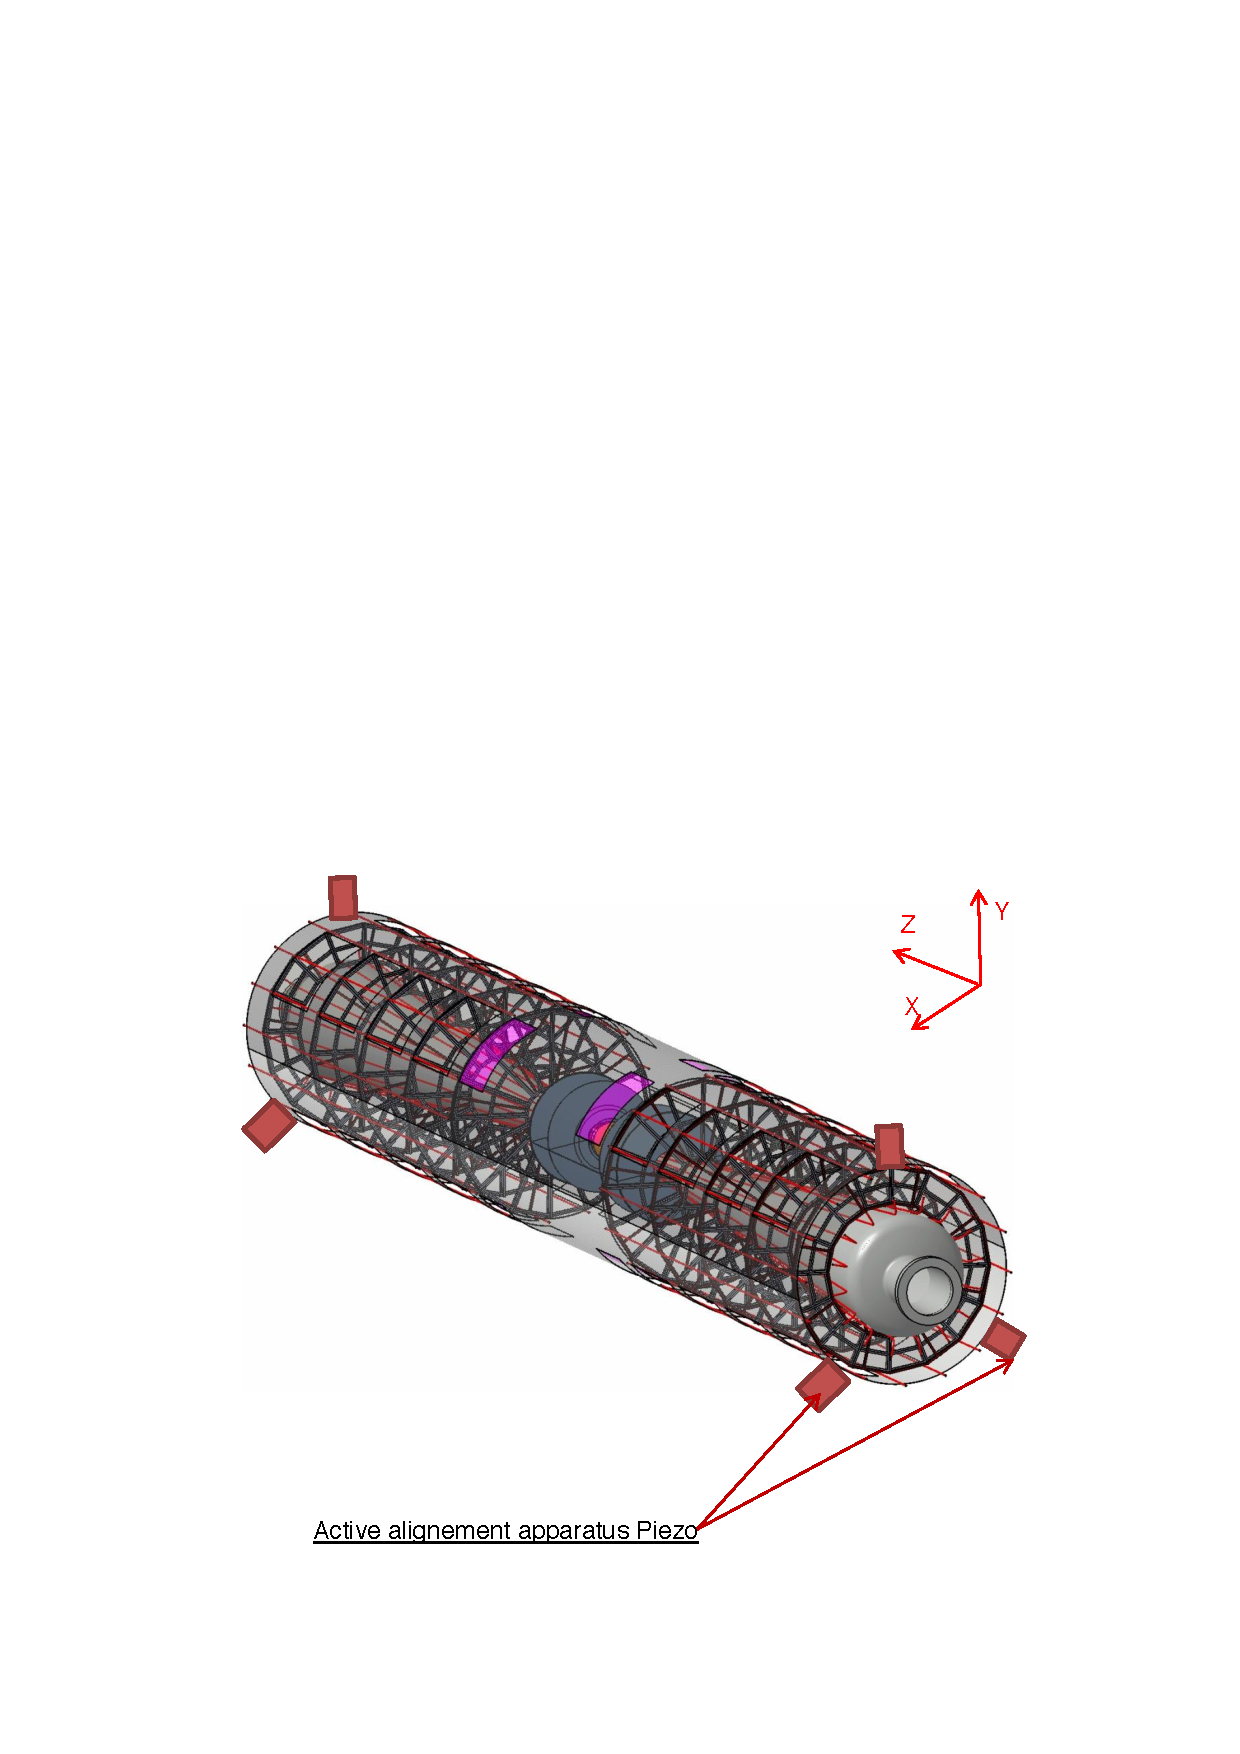
\includegraphics[width=0.8\hsize]{Integration/fig/Inner_Detector_Integration.pdf}
    \caption{Engineering design of the inner detector~\cite{ild:bib:inner_detector_integration}.}
    \label{ILD:fig:inner_detector_integration}
\end{figure}

\subsubsection{Electrical Services and Cooling}
A concept has been developed for the power scheme of the vertex detector (CMOS version), see Figure~\ref{ILD:fig:vtx_services}. Copper based power and control cables as well as optical fibres for the data readout connect the vertex detector with patch panels at either ends of the ISS. From here, the cables are routed as described in section~\ref{ild:sec:services} to the outside of the detector. An engineering design for the details of the cabling and patch panels inside the ISS is still pending. Figure~\ref{ILD:fig:si_services} shows the place holders for the cables in the current model. The vertex detector will be cooled using air flow cooling, where the cooling pipes also need to follow the general services paths.

\begin{figure}[h!]
    \centering
        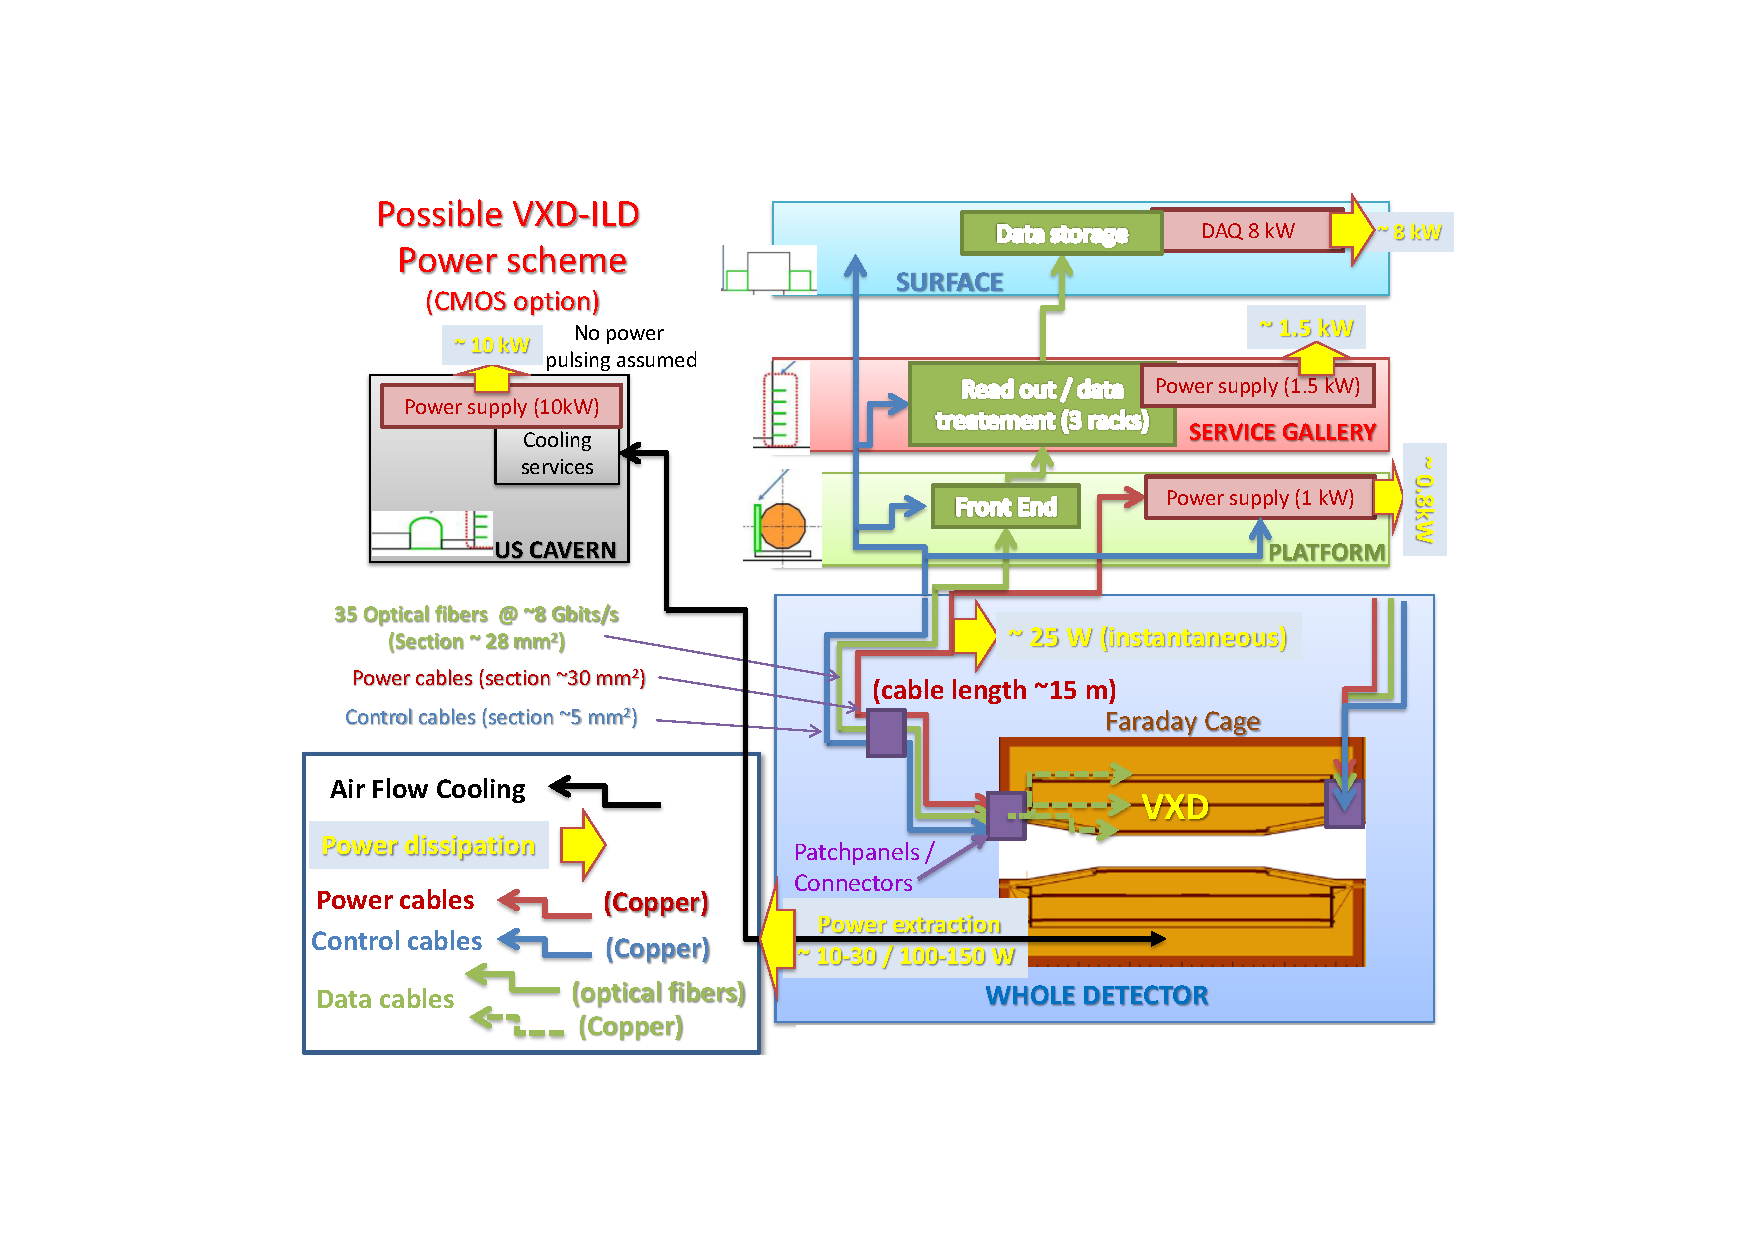
\includegraphics[width=0.8\hsize]{Integration/fig/VTX_services.pdf}
    \caption{Diagram of a power scheme for the vertex detector (CMOS option)~\cite{ild:bib:VTX_integration}.}
    \label{ILD:fig:vtx_services}
\end{figure}

\begin{figure}[h!]
    \centering
        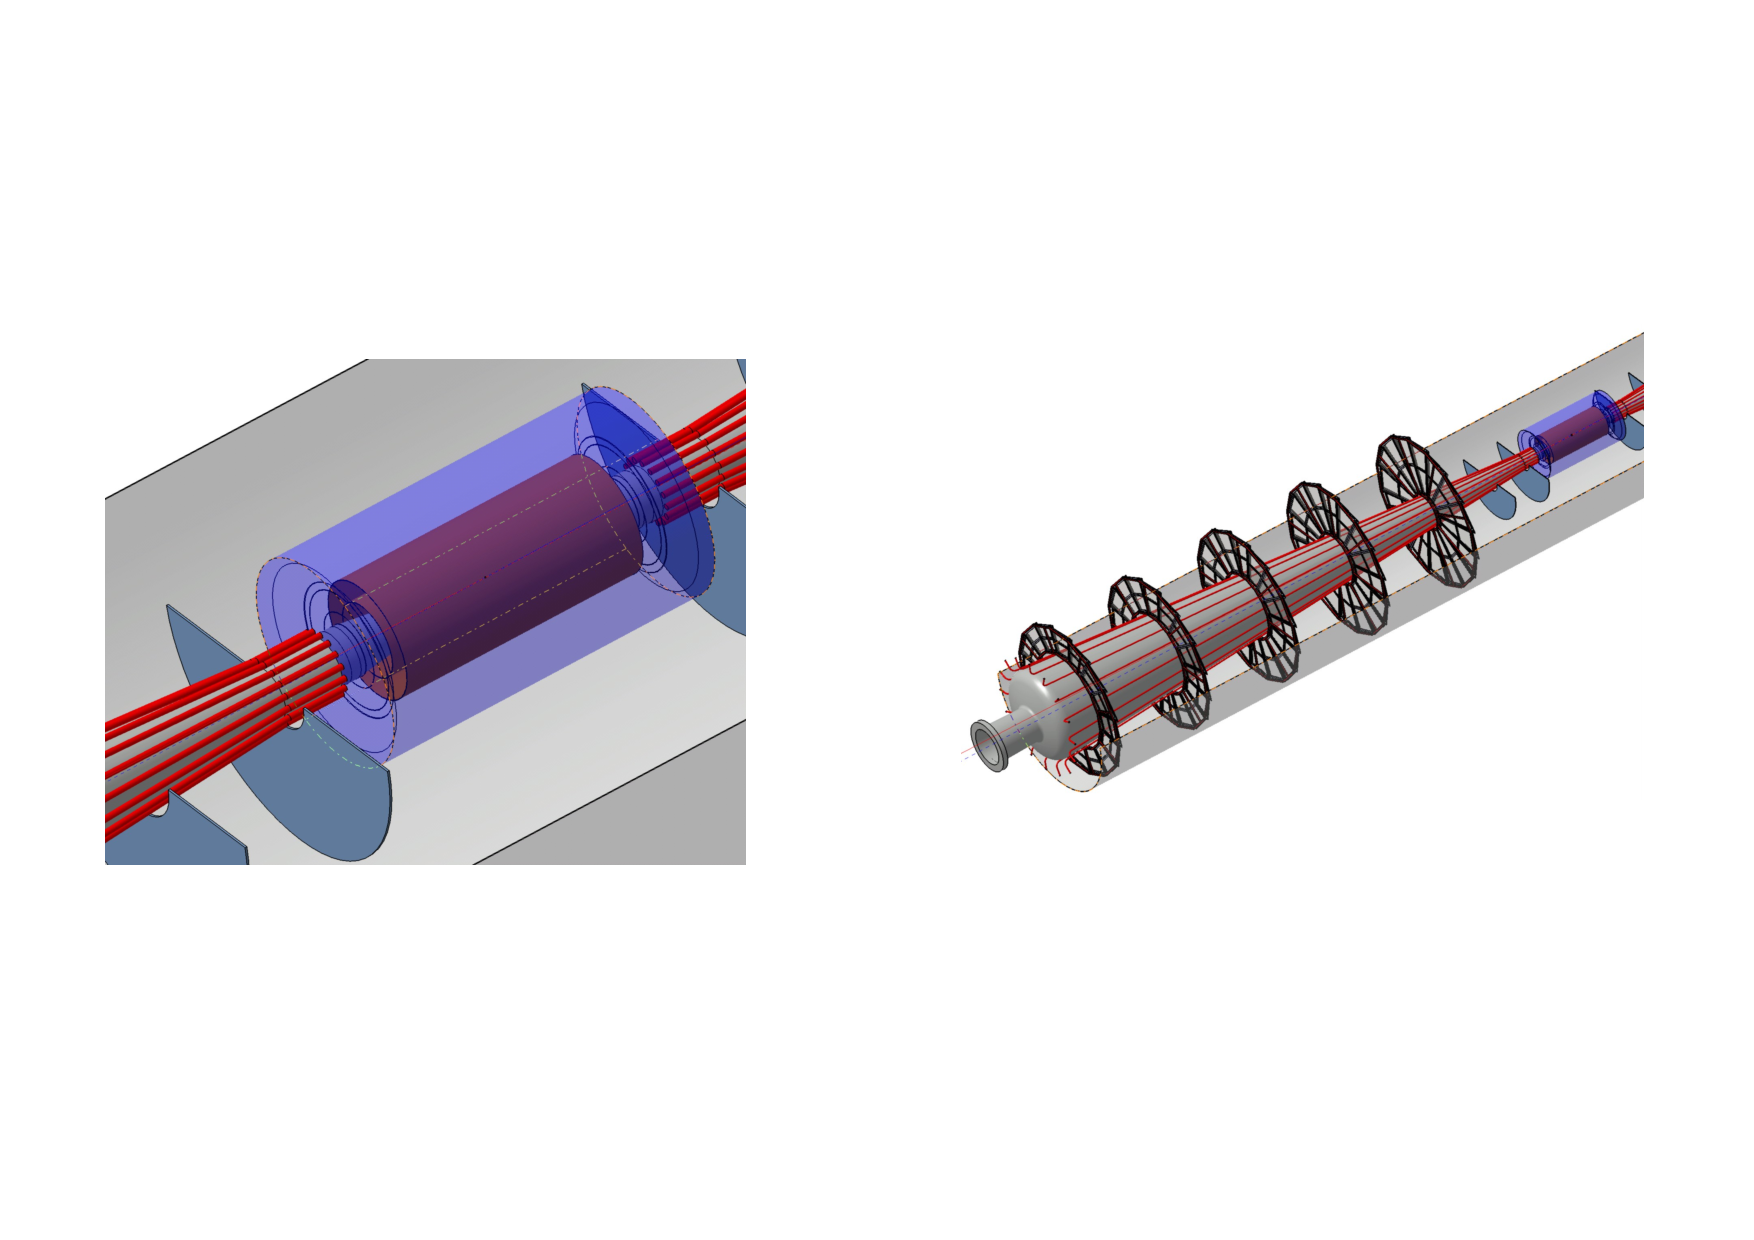
\includegraphics[width=0.8\hsize]{Integration/fig/SI_Services.pdf}
    \caption{Cable placeholders for the inner SI detectors (VTX, SIT, FTD)~\cite{ild:bib:SI_integration}.}
    \label{ILD:fig:si_services}
\end{figure}

\subsection{TPC Integration}

\subsubsection{Mechanical integration}

The mechanical integration of the TPC is still under study. Two possible concepts are being followed up. Either the TPC will be suspended directly from the solenoid cryostat with the help of carbon ribbons or support struts. Or it can be mounted to the absorber structure of the hadronic calorimeter. In the first case, the TPC would be decoupled from the mechanical properties of the calorimeters, at the price of having larger lever arms that might amplify vibrations. A longitudinal damping system would probably be required. In the second case, the lever arms would be much shorter, but the dynamic behaviour of the full system of the cryostat, hadronic and electomagnetic calorimeter as well as the TPC itself needs to be understood. 

\subsubsection{Electrical Services and Cooling}

The electrical services and the cooling pipes of the TPC start on both end plates and will be routed through gaps in the front-faces of the calorimeters, between the end-cap and barrel detectors (c.f.~Figure~\ref{ILD:fig:tpc_cables}). A cooling system based on 2-phase CO2 has been tested in 2014 and 2018 on a system of
7 Micromegas modules. Figure~\ref{ILD:fig:tpc_cooling} shows a solution with a 6-loop geometry. The external supplies of the TPC need to be accommodated in the detector environment: while a gas mixing and supply system will most probably be placed on the surface area, distribution sub-systems need to be closer to the detector, e.g.~on the detector platform. The high-voltage power supplies will be placed in the detector hall at reasonable cable-length distances. Figure~\ref{ILD:fig:tpc_interfaces} shows a schematic drawing of the TPC connections to the outer world.

\begin{figure}[h!]
    \centering
    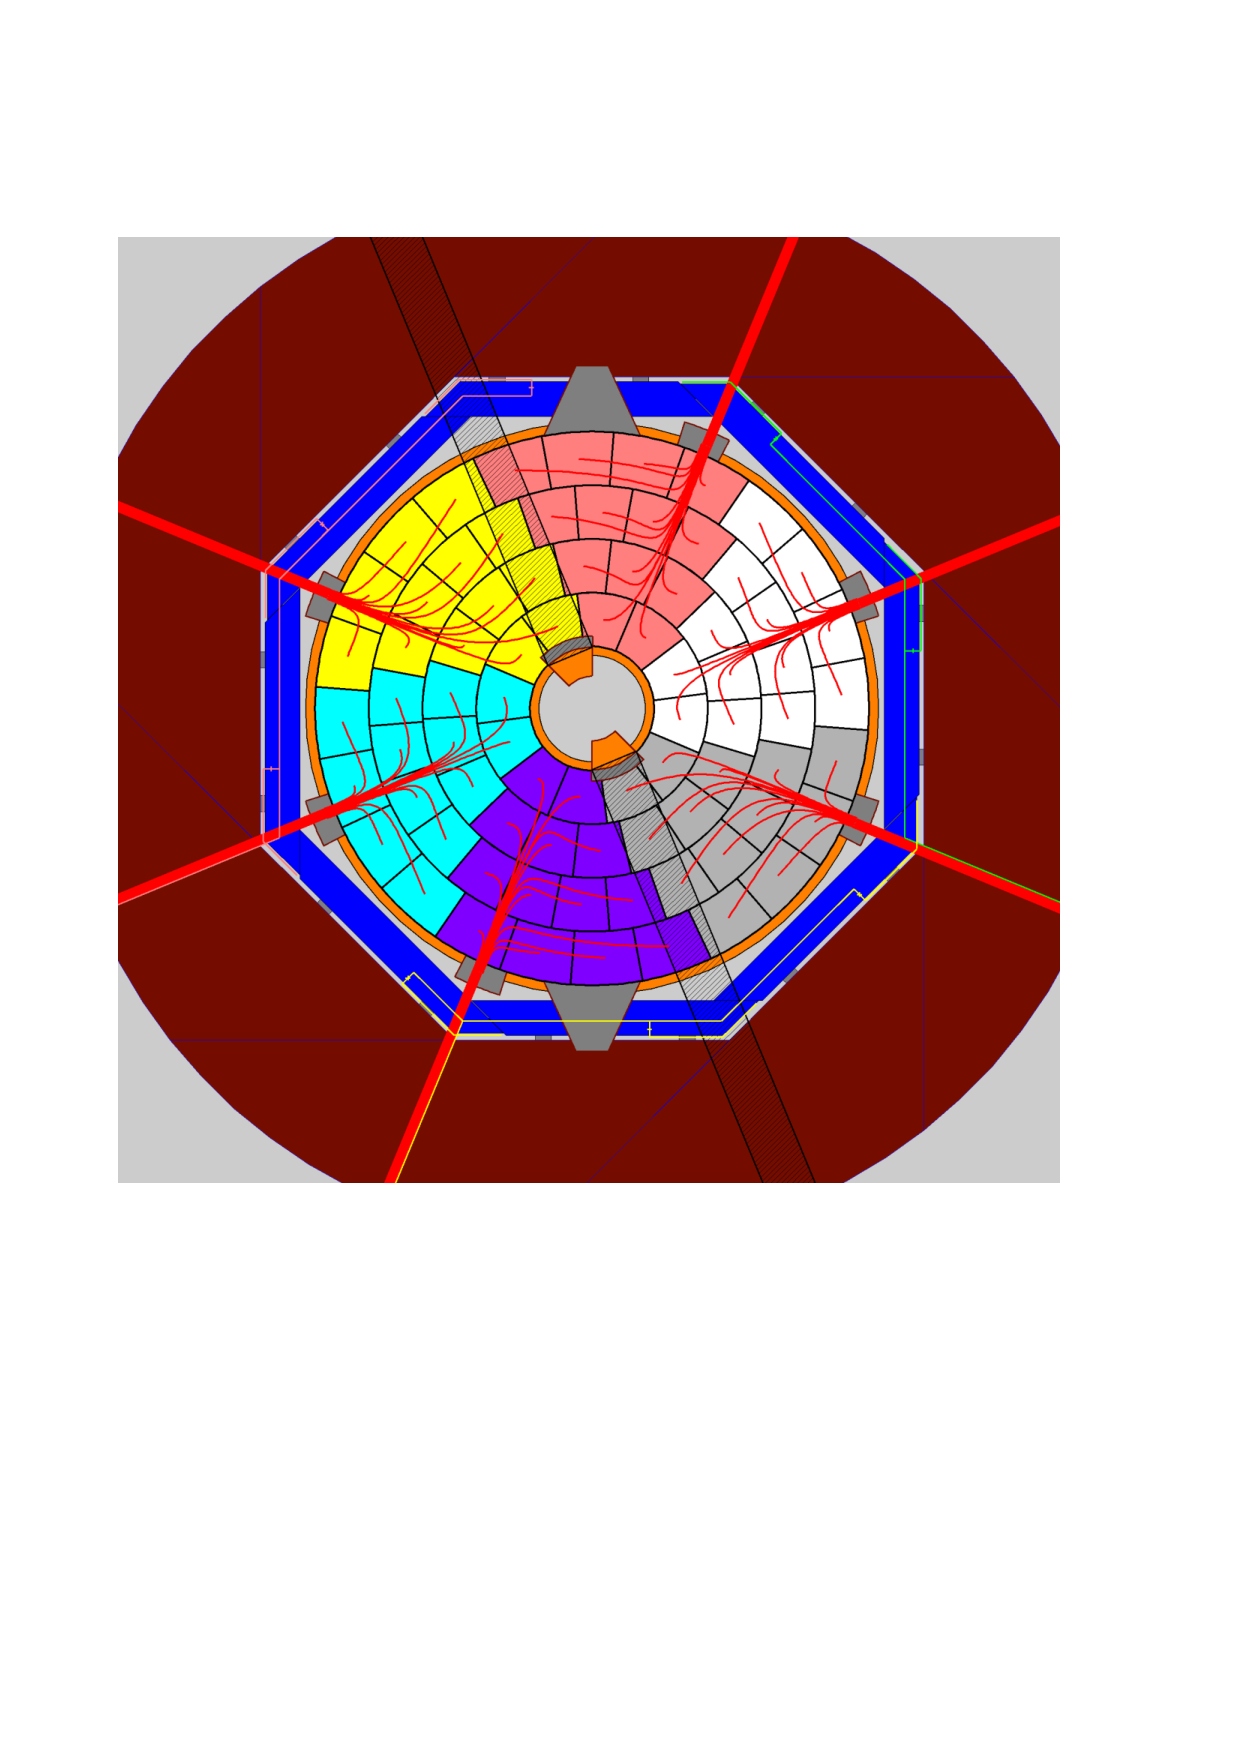
\includegraphics[width=0.6\hsize]{Integration/fig/TPC_Cables.pdf}
    \caption{Sketch of the cable paths on the front-end of the TPC~\cite{ild:bib:TPC_ICD}.}
    \label{ILD:fig:tpc_cables}
\end{figure}
\begin{figure}[h!]
    \centering
    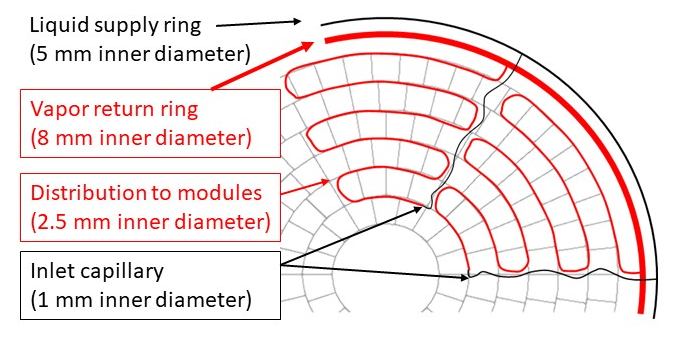
\includegraphics[width=1.0\hsize]{Integration/fig/TPC_Cooling_v2.png}
    \caption{Sketch of a TPC cooling system with tube routing on the TPC end plate. Figure courtesy of Bart Verlaat, Nikhef.}
    \label{ILD:fig:tpc_cooling}
\end{figure}

\begin{figure}[h!]
    \centering
    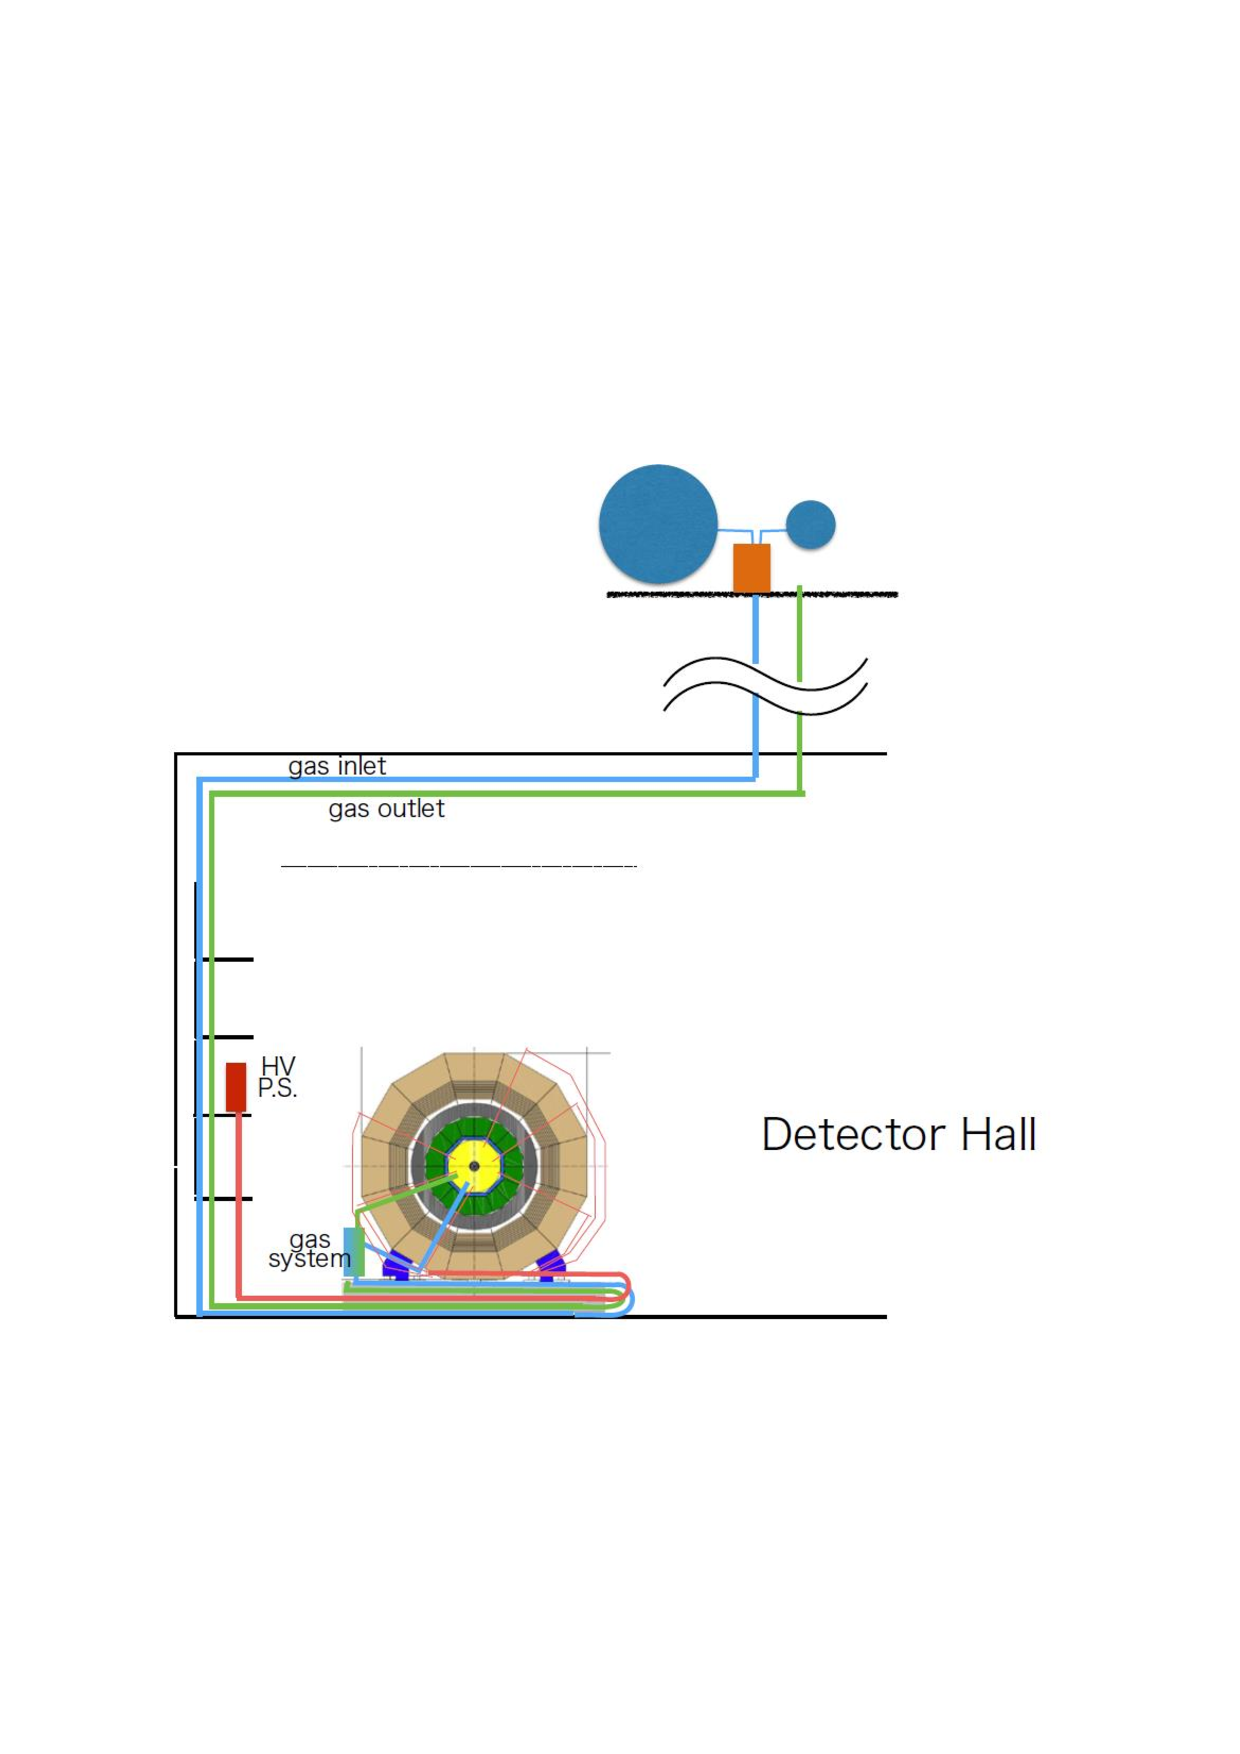
\includegraphics[width=1.0\hsize]{Integration/fig/TPC_Interfaces.pdf}
    \caption{Gas and HV interfaces of the TPC~\cite{ild:bib:TPC_ICD}.}
    \label{ILD:fig:tpc_interfaces}
\end{figure}


\subsection{Electromagnetic Calorimeters Integration}

\subsubsection{Mechanical Integration}

The two options under study for the ILD electromagnetic calorimeters, SiECAL and ScECAL, share the same mechanical design as shown in Figure~\ref{fig:det:ECAL}. The ECAL barrel consists of eight staves that are built from five modules each~(c.f.~figure~\ref{ILD:fig:ECAL_Mechanics}). The staves are supported from the HCAL barrel sections. The ECAL endcaps are supported from the HCAL endcap detector.
\begin{figure}[h]
    \centering
        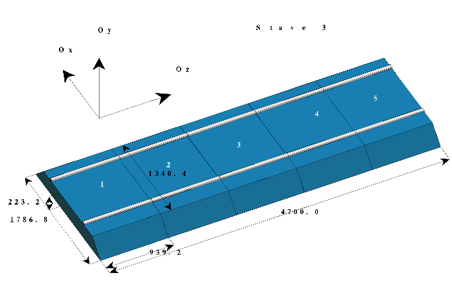
\includegraphics[width=0.5\hsize]{Integration/fig/ECAL_Stave.png}
        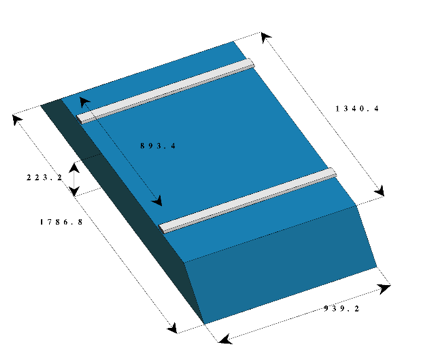
\includegraphics[width=0.3\hsize]{Integration/fig/ECAL_Module.png}
    \caption{ECAL stave and module~\cite{ild:bib:SiECAL_ICD}}
    \label{ILD:fig:ECAL_Mechanics}
\end{figure}

\subsubsection{SiECAL Electrical Services and Cooling}

A detailed integrated design of the SiECAL electrical services and of the cooling system has been developed. Figure~\ref{ILD:fig:siecal_services} shows a close-up view of the upper side of a SiECAL module. The front-end electronics is located at the end of the readout slabs. The services are collected at dedicated hubs for a full column of slabs ("SiECAL Hub2" in the Figure). The service from the column hubs are collected at one central hub for each full stave ("SiECAL Hub1"). Figure~\ref{ILD:fig:siecal_block_diagram} shows a block diagram of the electrical services for the SiECAL and the connections from "Hub1" to the outside power supplies, to the common clock and the DAQ. 

\begin{figure}[h!]
    \centering
        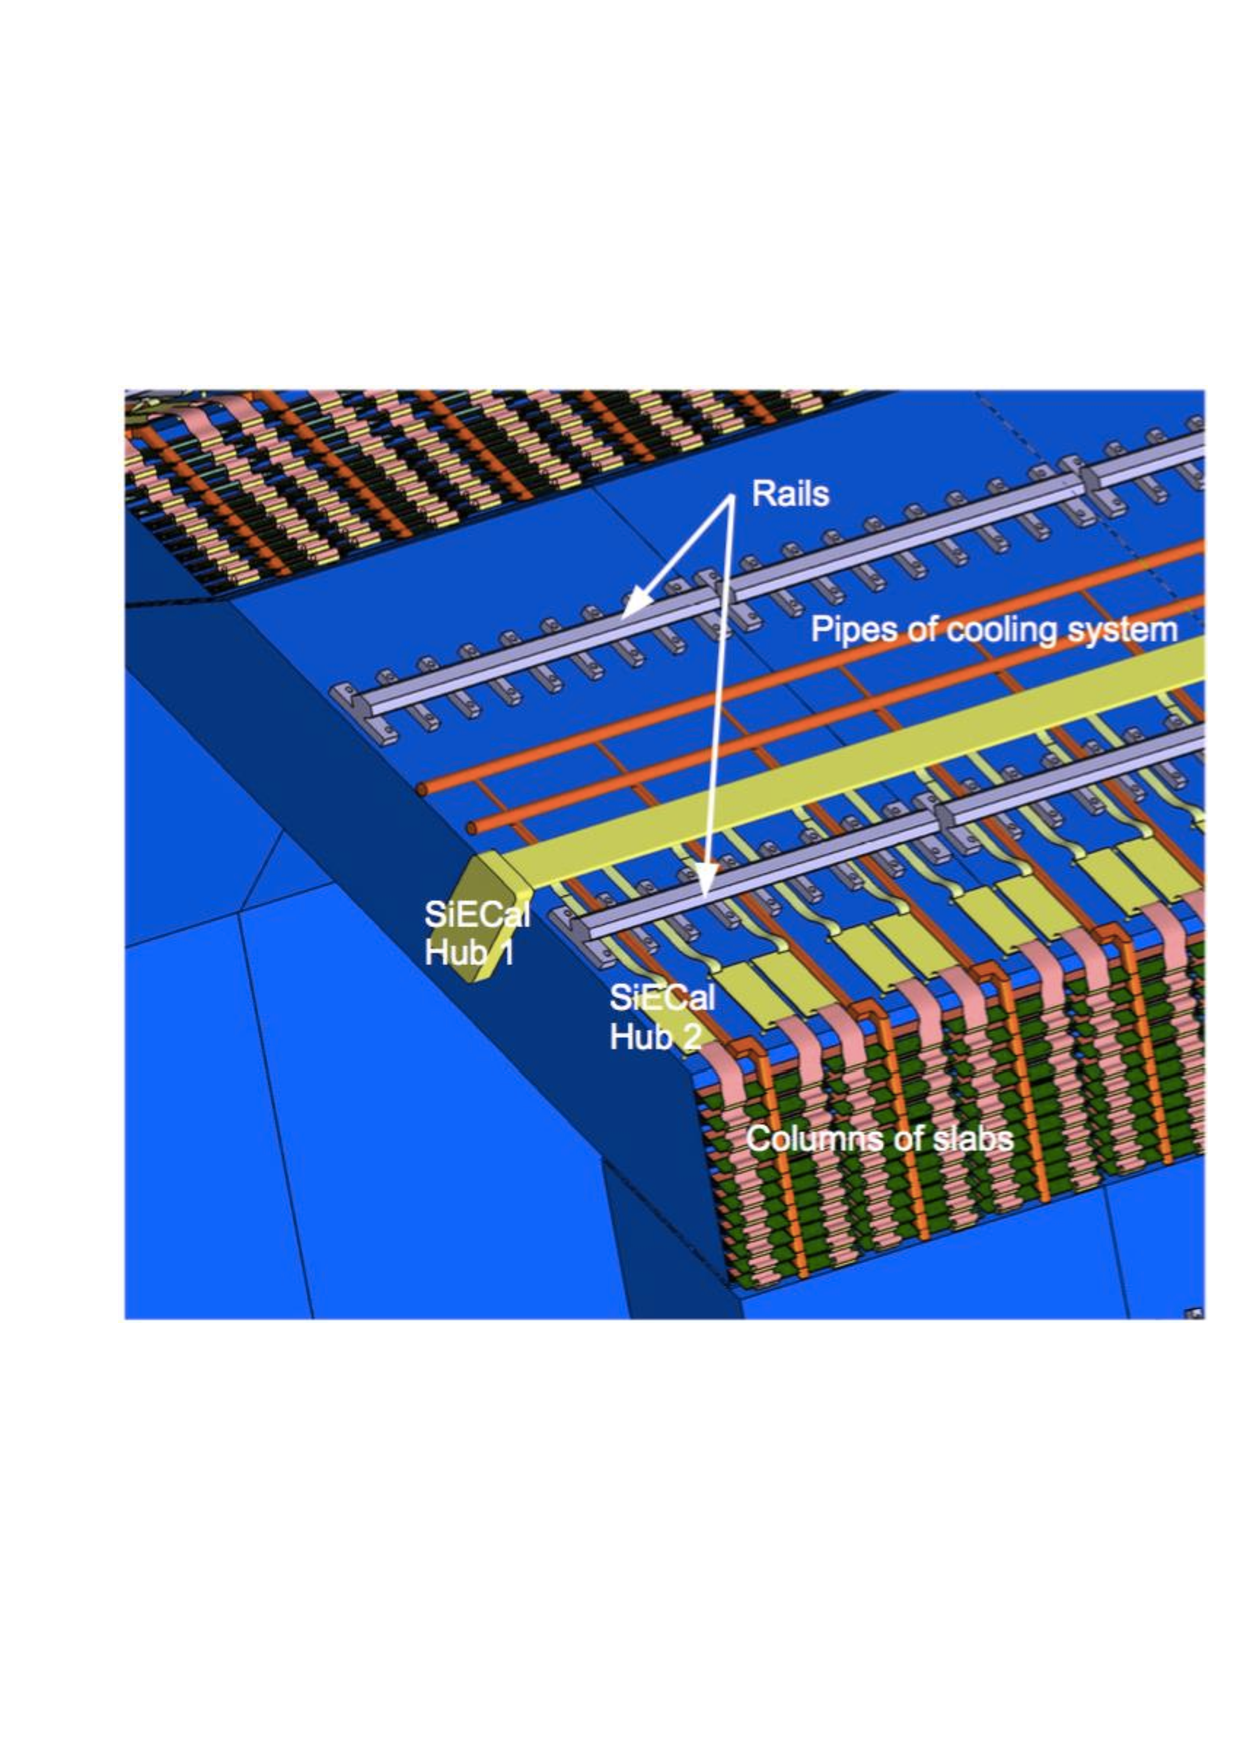
\includegraphics[width=0.6\hsize]{Integration/fig/SiECAL_Services.pdf}
    \caption{Services on an SiECAL module~\cite{ild:bib:SiECAL_ICD}.}
    \label{ILD:fig:siecal_services}
\end{figure}

\begin{figure}[h!]
    \centering
        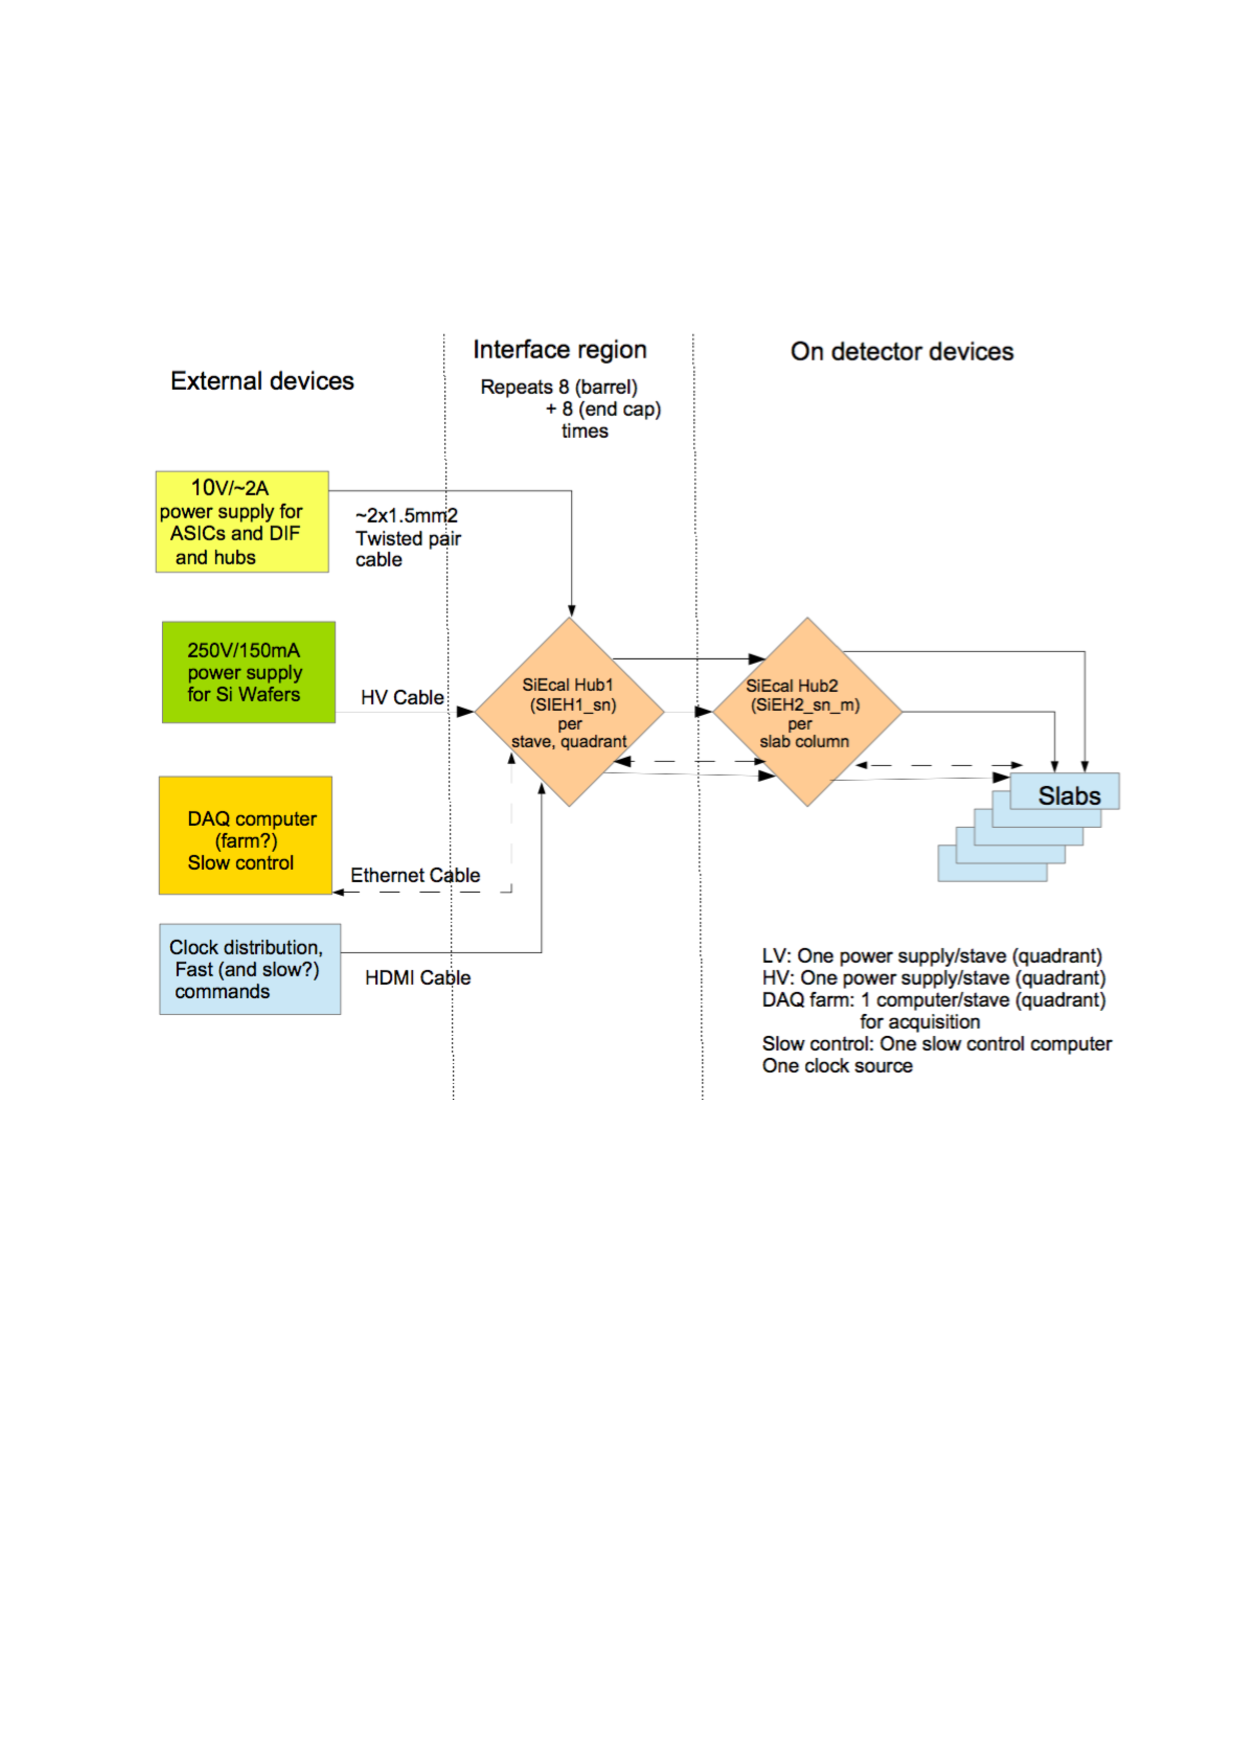
\includegraphics[width=0.8\hsize]{Integration/fig/SiECAL_Block_Diagram.pdf}
    \caption{Block diagram of the electrical services for the SiECAL~\cite{ild:bib:SiECAL_ICD}.}
    \label{ILD:fig:siecal_block_diagram}
\end{figure}

A conceptual design for the SiECAL cooling system is shown in Figure~\ref{ILD:fig:siecal_cooling}. The system foresees leakless water cooling, where a cooling station would be located outside of the ILD detector in the underground area. The water will be distributed via an hierarchical system of cooling lines ("A" to "F") to the barrel and endcap detectors.

\begin{figure}[h!]
    \centering
        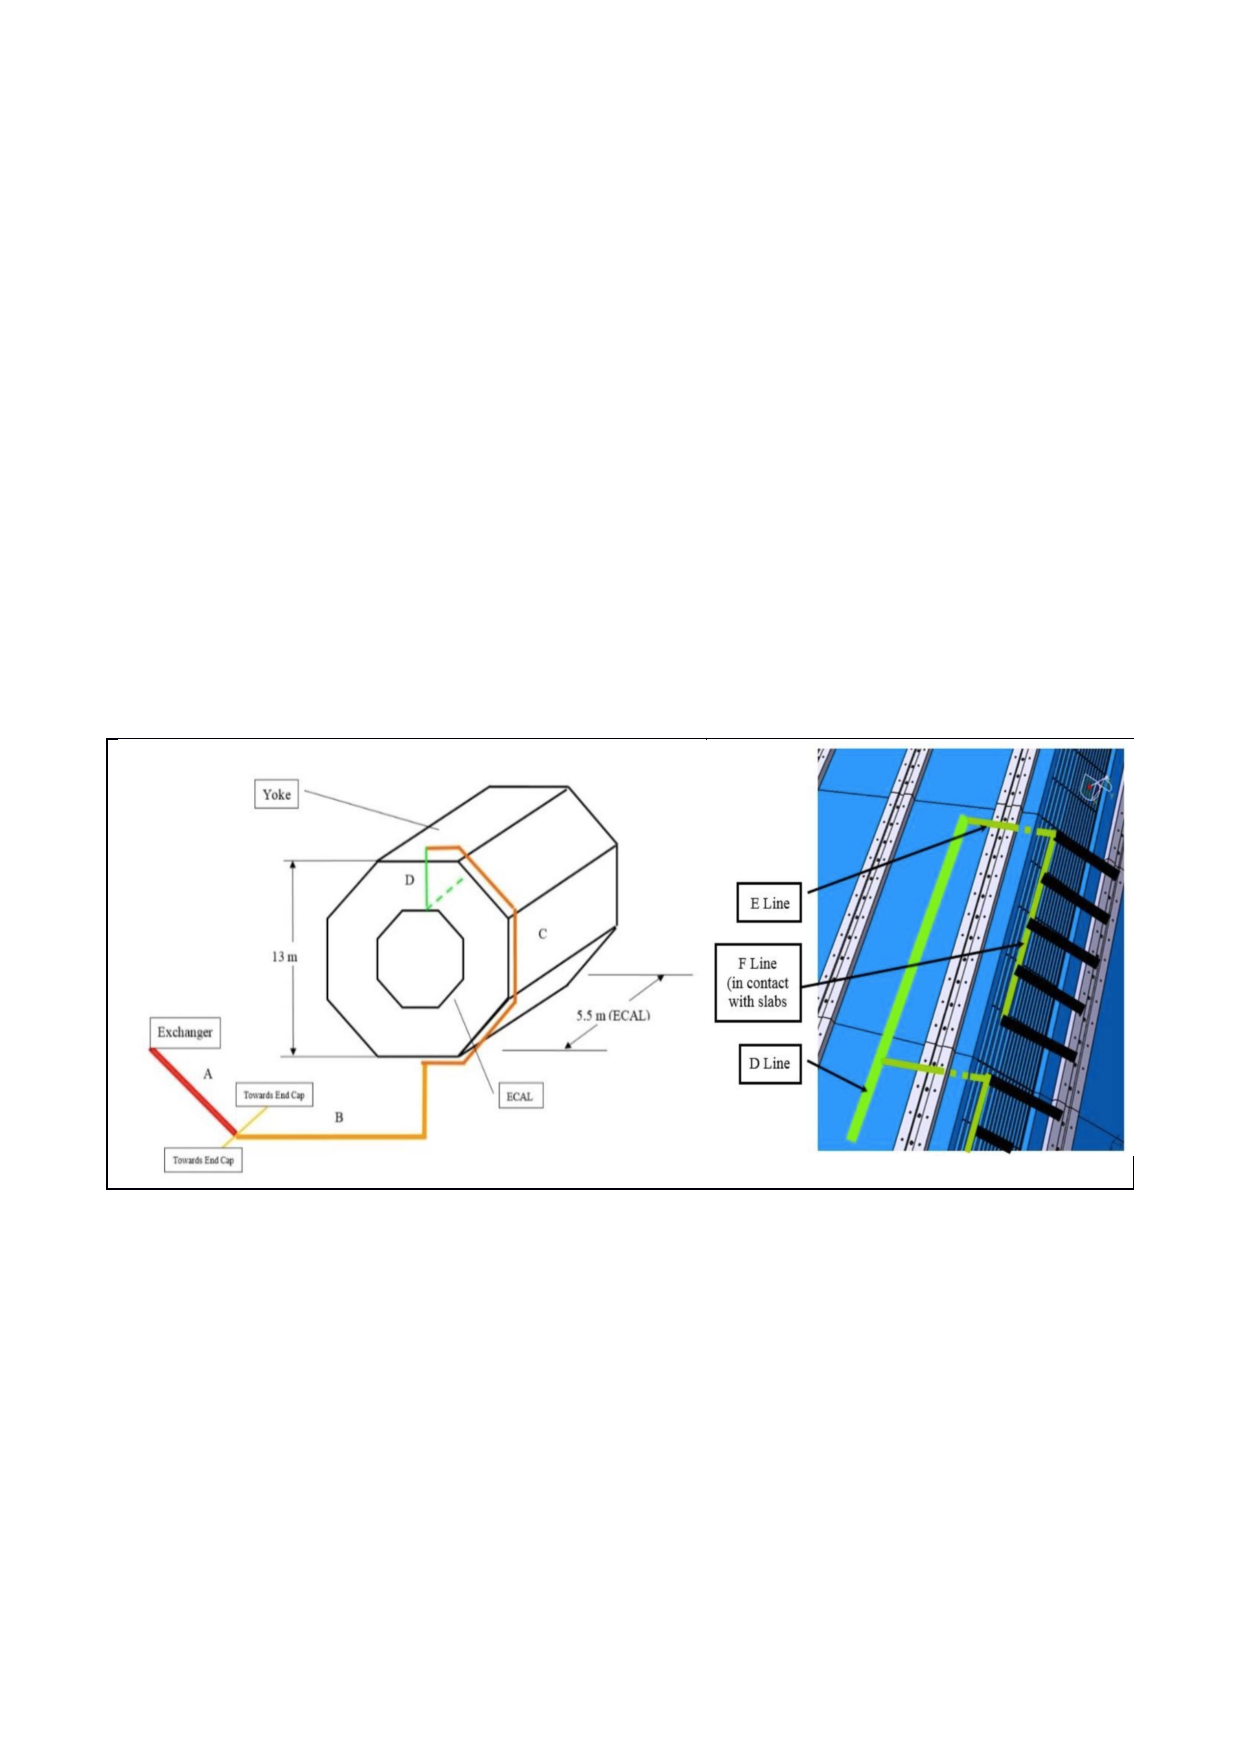
\includegraphics[width=0.8\hsize]{Integration/fig/SiECAL_Cooling.pdf}
    \caption{Conceptual design of the SiECAL cooling system~\cite{ild:bib:SiECAL_ICD}.}
    \label{ILD:fig:siecal_cooling}
\end{figure}

\subsubsection{ScECAL Electrical Services}
The distribution of the electrical services for the ScECAL is very similar to the SiECAL case. Figure~\ref{ILD:fig:scecal_block_diagram} show a block diagram of the service distributions. Also in this case, two series of hubs are planned, one for each stave and one for each column of slabs, to distribute HV and signals accordingly.
\begin{figure}[h!]
    \centering
        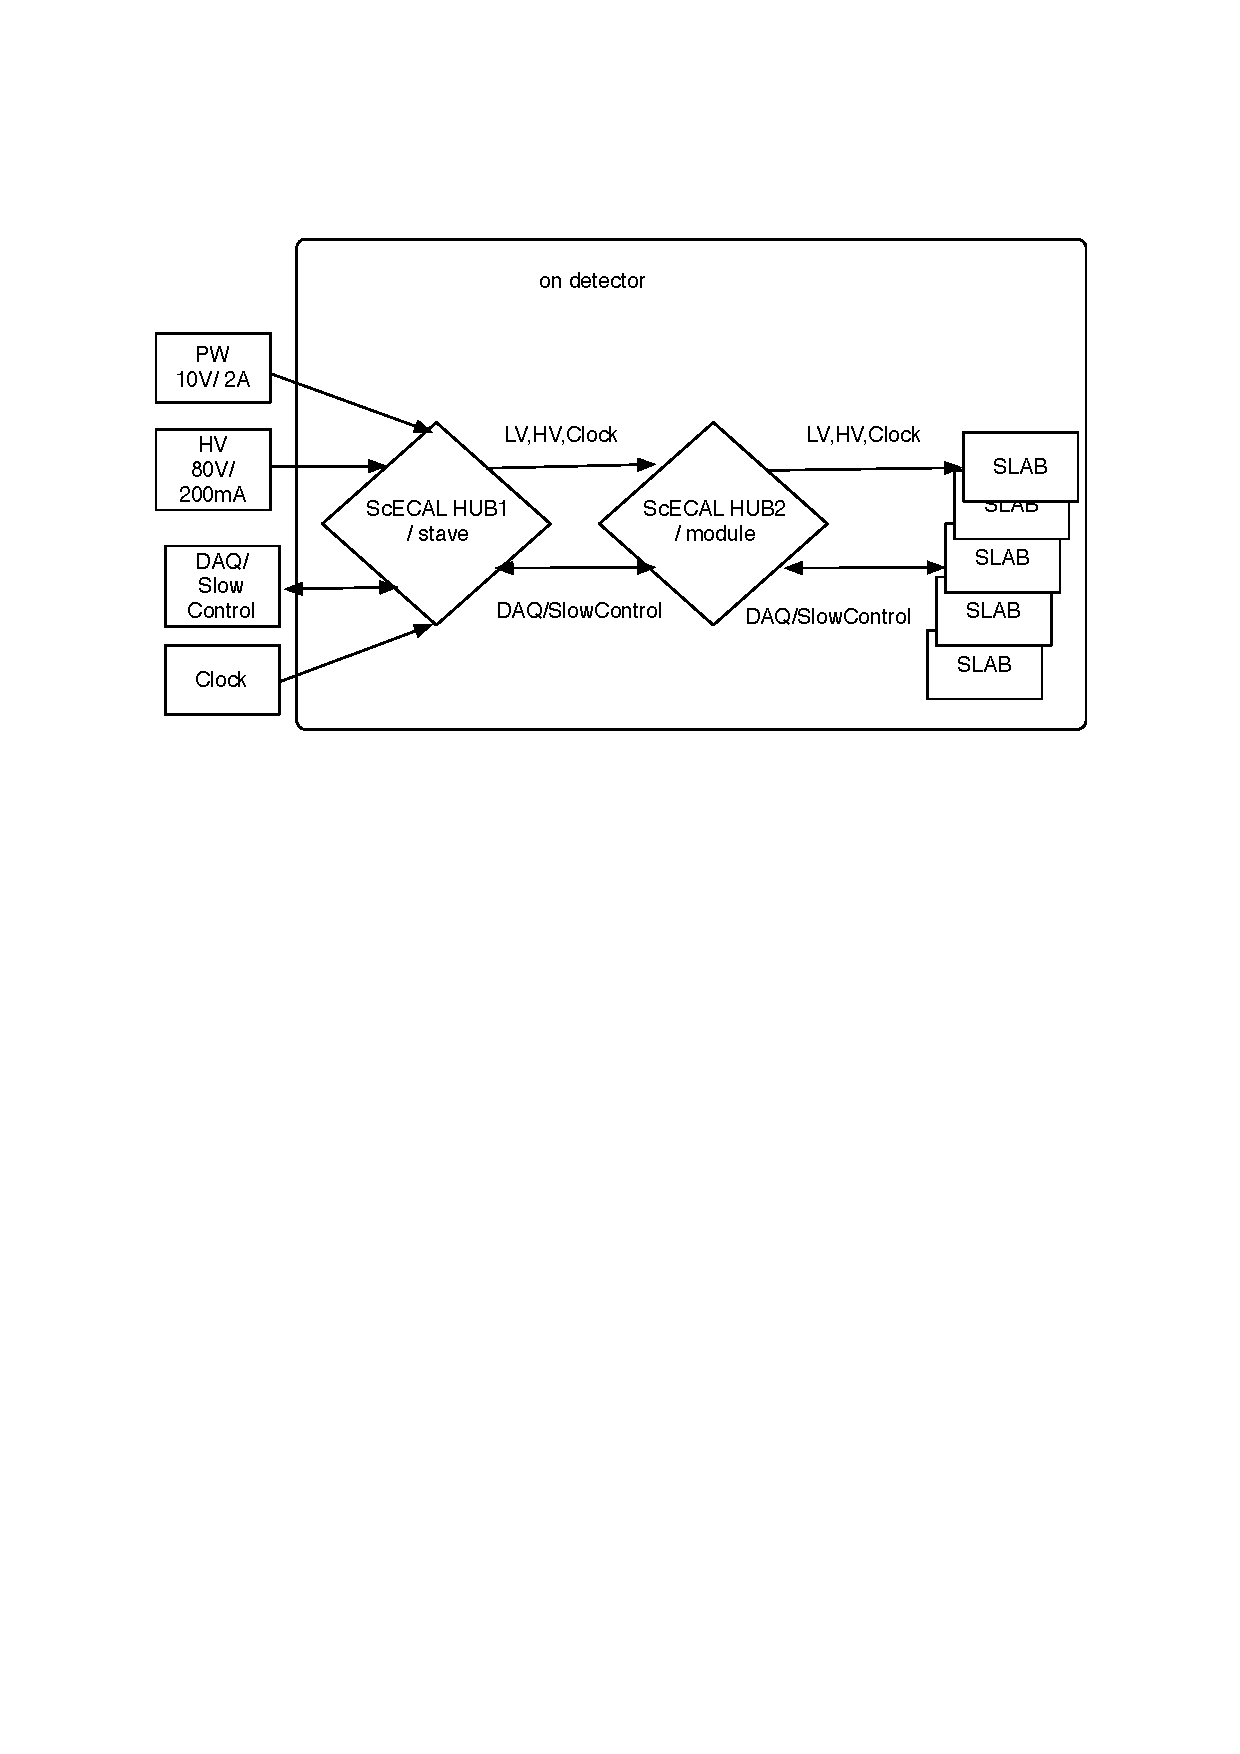
\includegraphics[width=0.8\hsize]{Integration/fig/ScECAL_Block_Diagram.pdf}
    \caption{Block diagram of the electrical services for the ScECAL~\cite{ild:bib:ScECAL_ICD}.}
    \label{ILD:fig:scecal_block_diagram}
\end{figure}


\subsection{Hadronic Calorimeters Integration}
\subsubsection{Mechanical Integration}

Two absorber structures are under study for ILD, the so-called "TESLA" and "Videau" structures~(c.f.~Figure~\ref{fig:det:HCAL}). The main differences from the viewpoint of the detector integration are the mechanical behaviour, further discussed in section~\ref{ild:sec:mechanical_structures}, and the layout of the detector electrical and cooling services. The analogue AHCAL and the semi-digital SDHCAL can be adapted to both mechanical structures. In practice, the AHCAL has been designed with the "TESLA" structure in mind, while the SDHCAL is optimised for the "Videau" case.

\subsubsection{AHCAL Electrical Services and Cooling}
An engineering model of the AHCAL barrel section in the "TESLA" structure has been designed and is shown in Figure~\ref{ILD:fig:ahcal_module_services}. Eight of these modules form a ring, two rings form the barrel detector. The active layers are read out via electronic boards that are located on the outside of the absorber structure. The data concentrators and power interfaces are accessible when the endcaps of the ILD detector are open.  
\begin{figure}[h!]
    \centering
        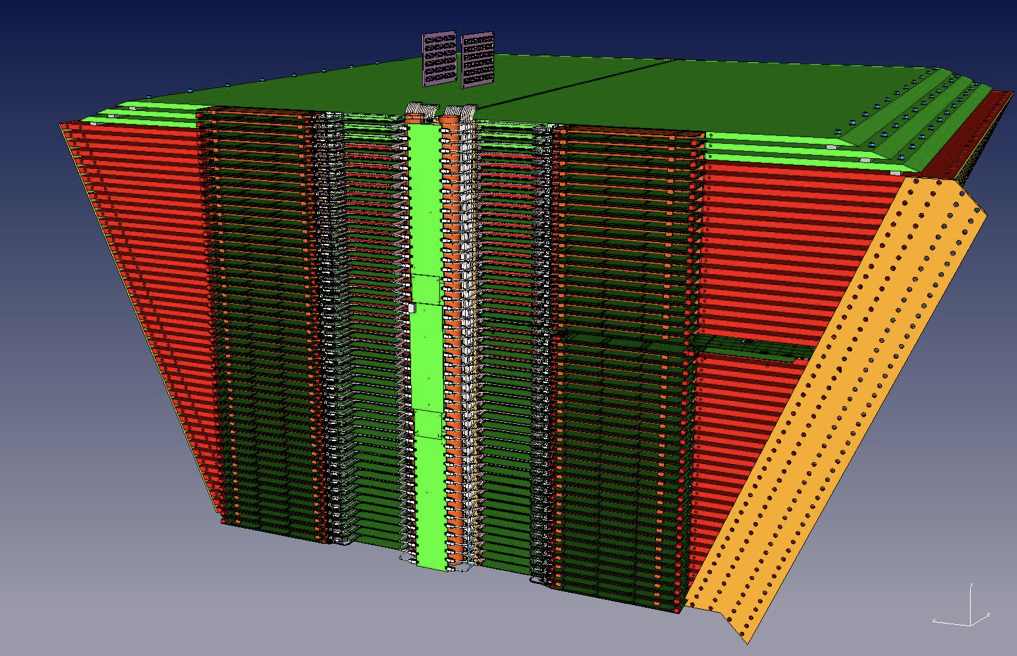
\includegraphics[width=0.8\hsize]{Integration/fig/AHCAL_Module_Services.png}
    \caption{Engineering design of an AHCAL module with electrical and cooling services. Only one instrumented layer is shown for the wedge shape outer parts of the module.1}
    \label{ILD:fig:ahcal_module_services}
\end{figure}
A close-up of the data concentator boards, the electrical services and the cooling system is shown in Figure~\ref{ILD:fig:ahcal_services_closeup}. This service concept has been implemented and successfully used with the AHCAL prototype, Fig.~\ref{fig:AHCAL-TileProto}. The electrical and cooling lines of ECAL, AHCAL, the TPC and the inner detector are routed via the gaps in the AHCAL front between the barrel and the endcap detector, as shown in Figure~\ref{ILD:fig:barrel_services}. 
\begin{figure}[h!]
    \centering
        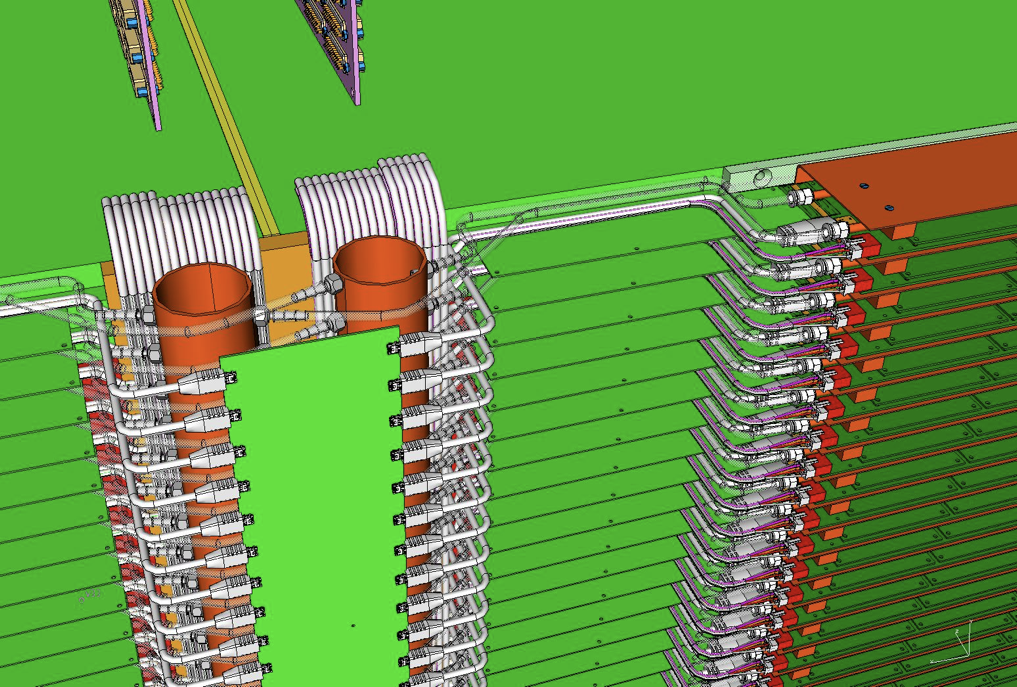
\includegraphics[width=0.9\hsize]{Integration/fig/AHCAL_Services_Closeup.png}
    \caption{AHCAL module front face with readout boards, cables and cooling lines.}
    \label{ILD:fig:ahcal_services_closeup}
\end{figure}
\begin{figure}[h!]
    \centering
        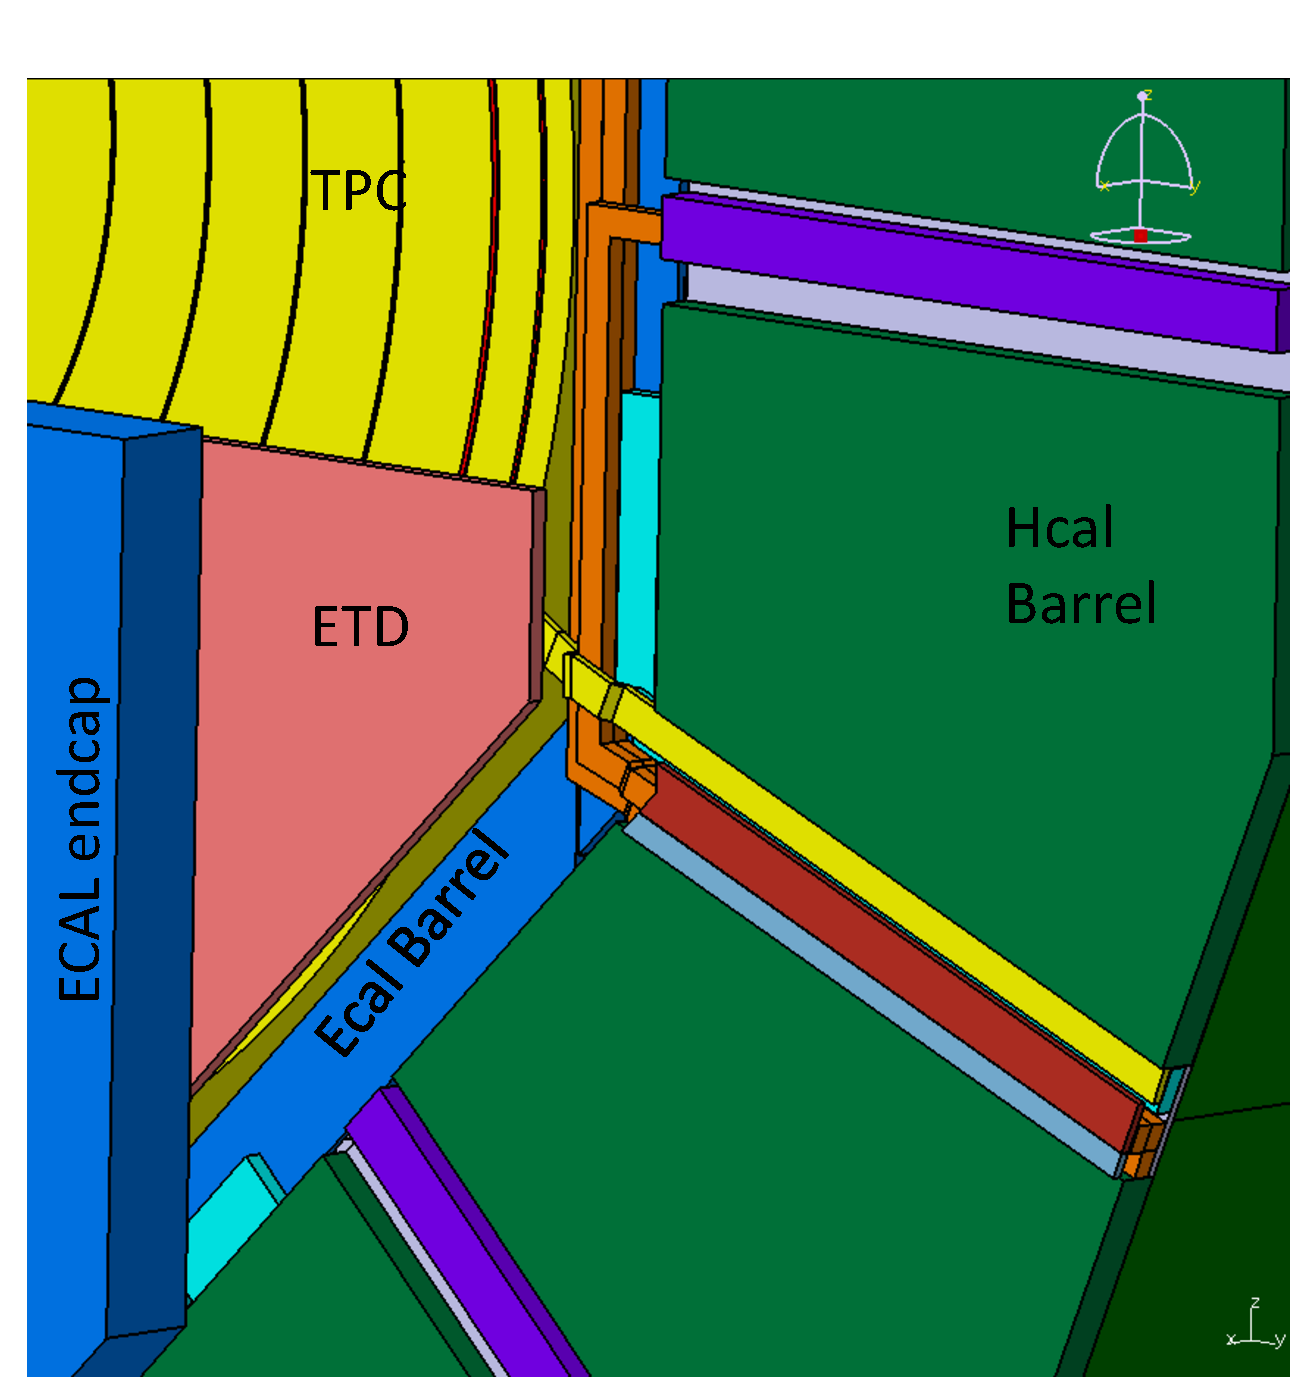
\includegraphics[width=0.7\hsize]{Integration/fig/Barrel_Services.pdf}
    \caption{Service paths on the AHCAL barrel front. The domain tagged "ETD" corresponds to an empty space following removal of the Endcap Tracking Detector from the ILD baseline design (section 5.1.2).}
    \label{ILD:fig:barrel_services}
\end{figure}
\subsubsection{SDHCAL Electrical Services and Cooling}
The SDHCAL barrel detector consists of three or five rings of eight wedge-shaped modules in the Videau configuration. As the active layers are installed from the outside of the barrel structures, access requires the removal of the respective barrel rings from the detector solenoid. The cables and cooling services run on the outside of each module to the barrel front face, as shown in Figure~\ref{ILD:fig:sdcal_module_services}. The SDHCAL services are routed around the detector solenoid to the outside. The services of the inner detector, the ECAL and the TPC can be routed on the front side of the SDHCAL barrel detector, as shown in Figure~\ref{ILD:fig:sdhcal_barrel_services}.
\begin{figure}[h!]
    \centering
        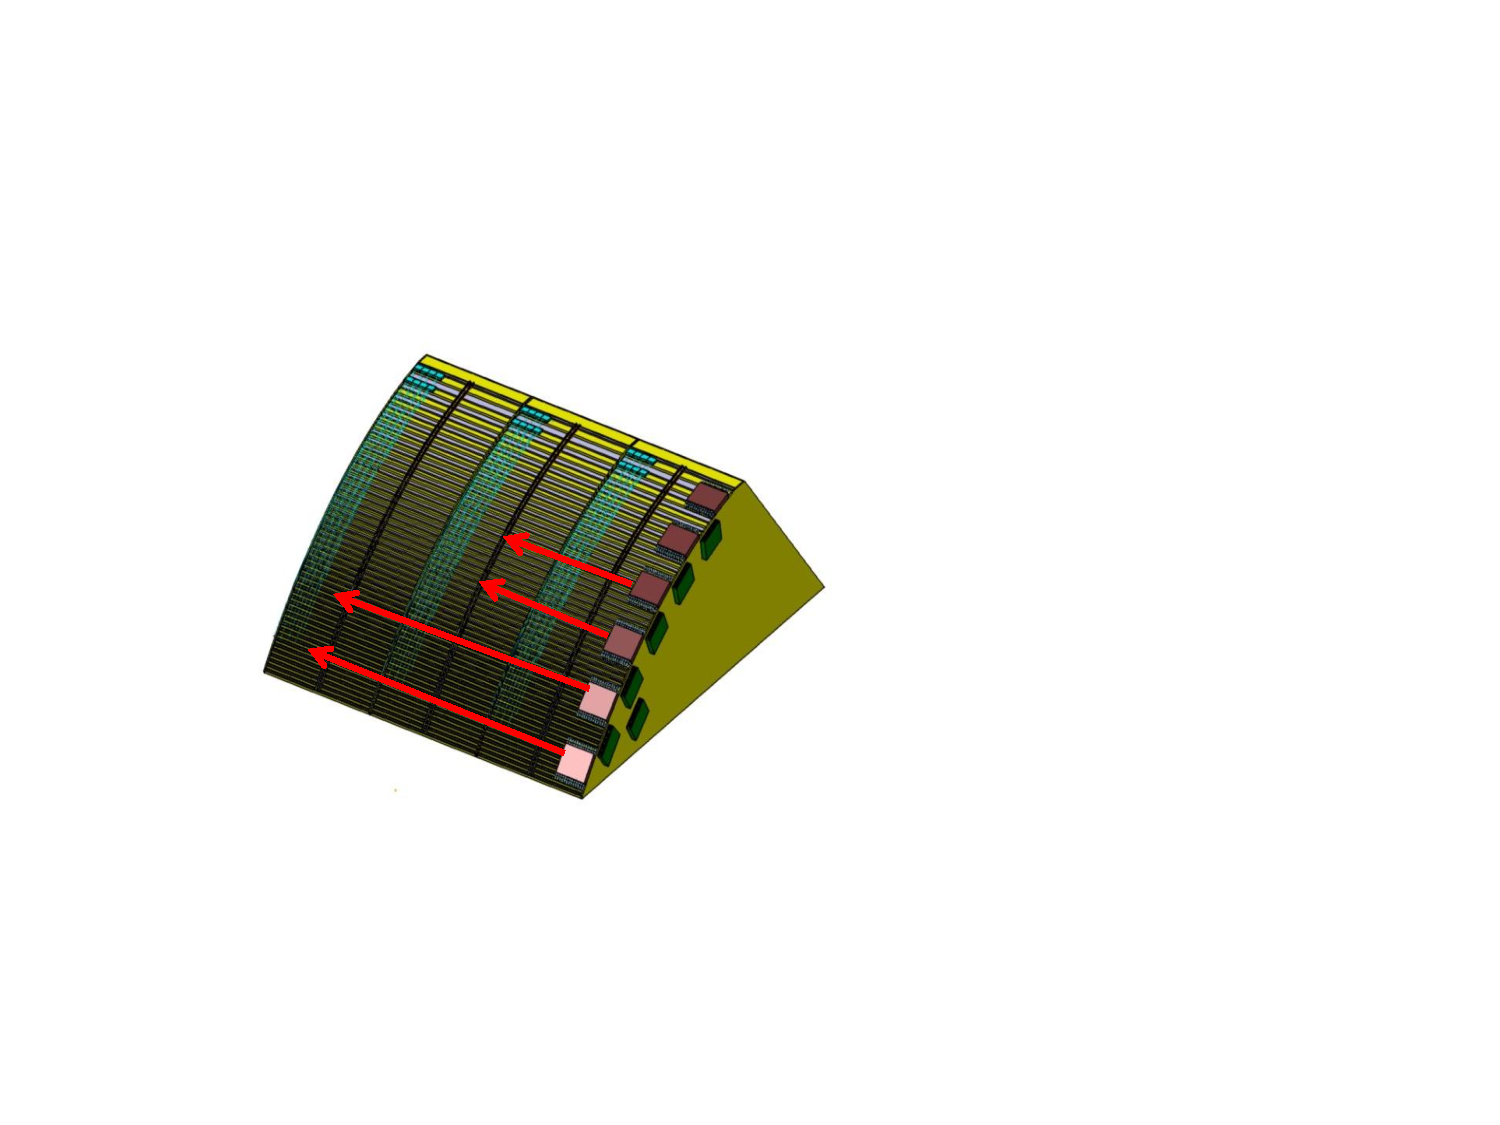
\includegraphics[width=0.8\hsize]{Integration/fig/SDHCAL_Module_Services.pdf}
    \caption{SDHCAL module with readout boards, cables and cooling lines.}
    \label{ILD:fig:sdcal_module_services}
\end{figure}
\begin{figure}[h!]
    \centering
        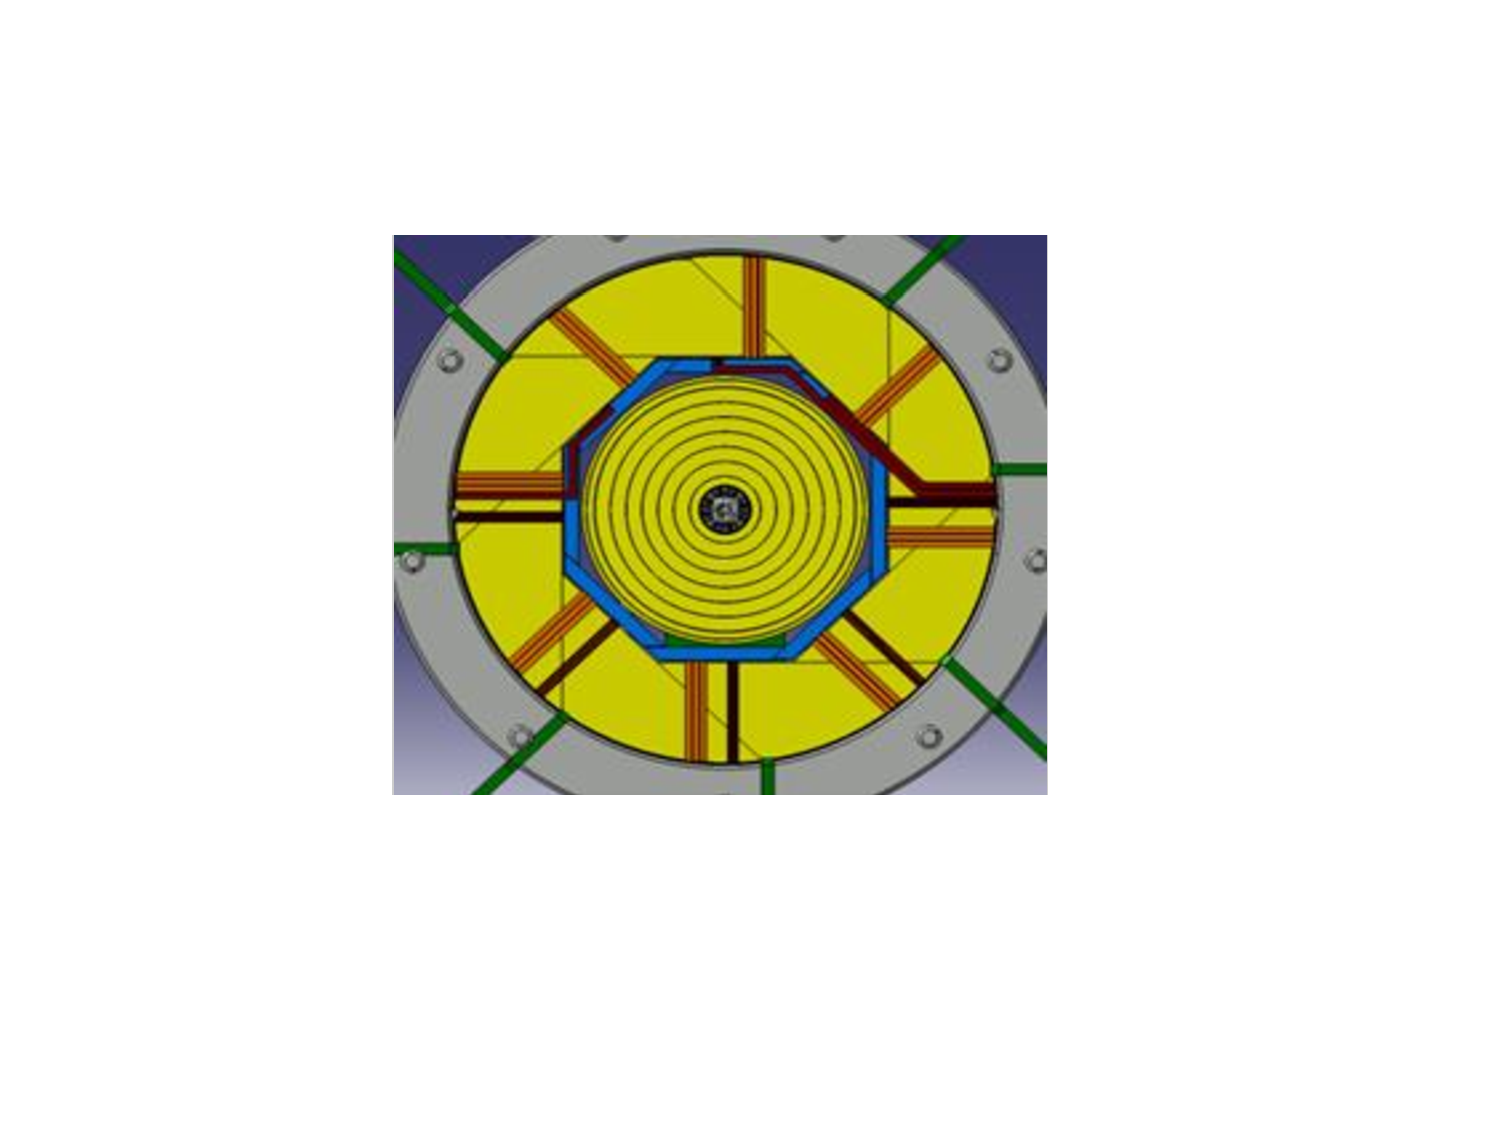
\includegraphics[width=0.8\hsize]{Integration/fig/SDHCAL_Barrel_Services.pdf}
    \caption{Service paths on the SDHCAL barrel front.}
    \label{ILD:fig:sdhcal_barrel_services}
\end{figure}

%\subsection{Yoke/Muon Integration}

\subsection{Very Forward System Integration}
The very forward systems, BeamCal, LumiCal and LHCal, are carried by the support structure for the final focus quadrupole QD0. Figure~\ref{ILD:fig:vfs_integration} shows the mechanical layout and the conceptual service paths of the forward calorimeters.
\begin{figure}[h!]
    \centering
    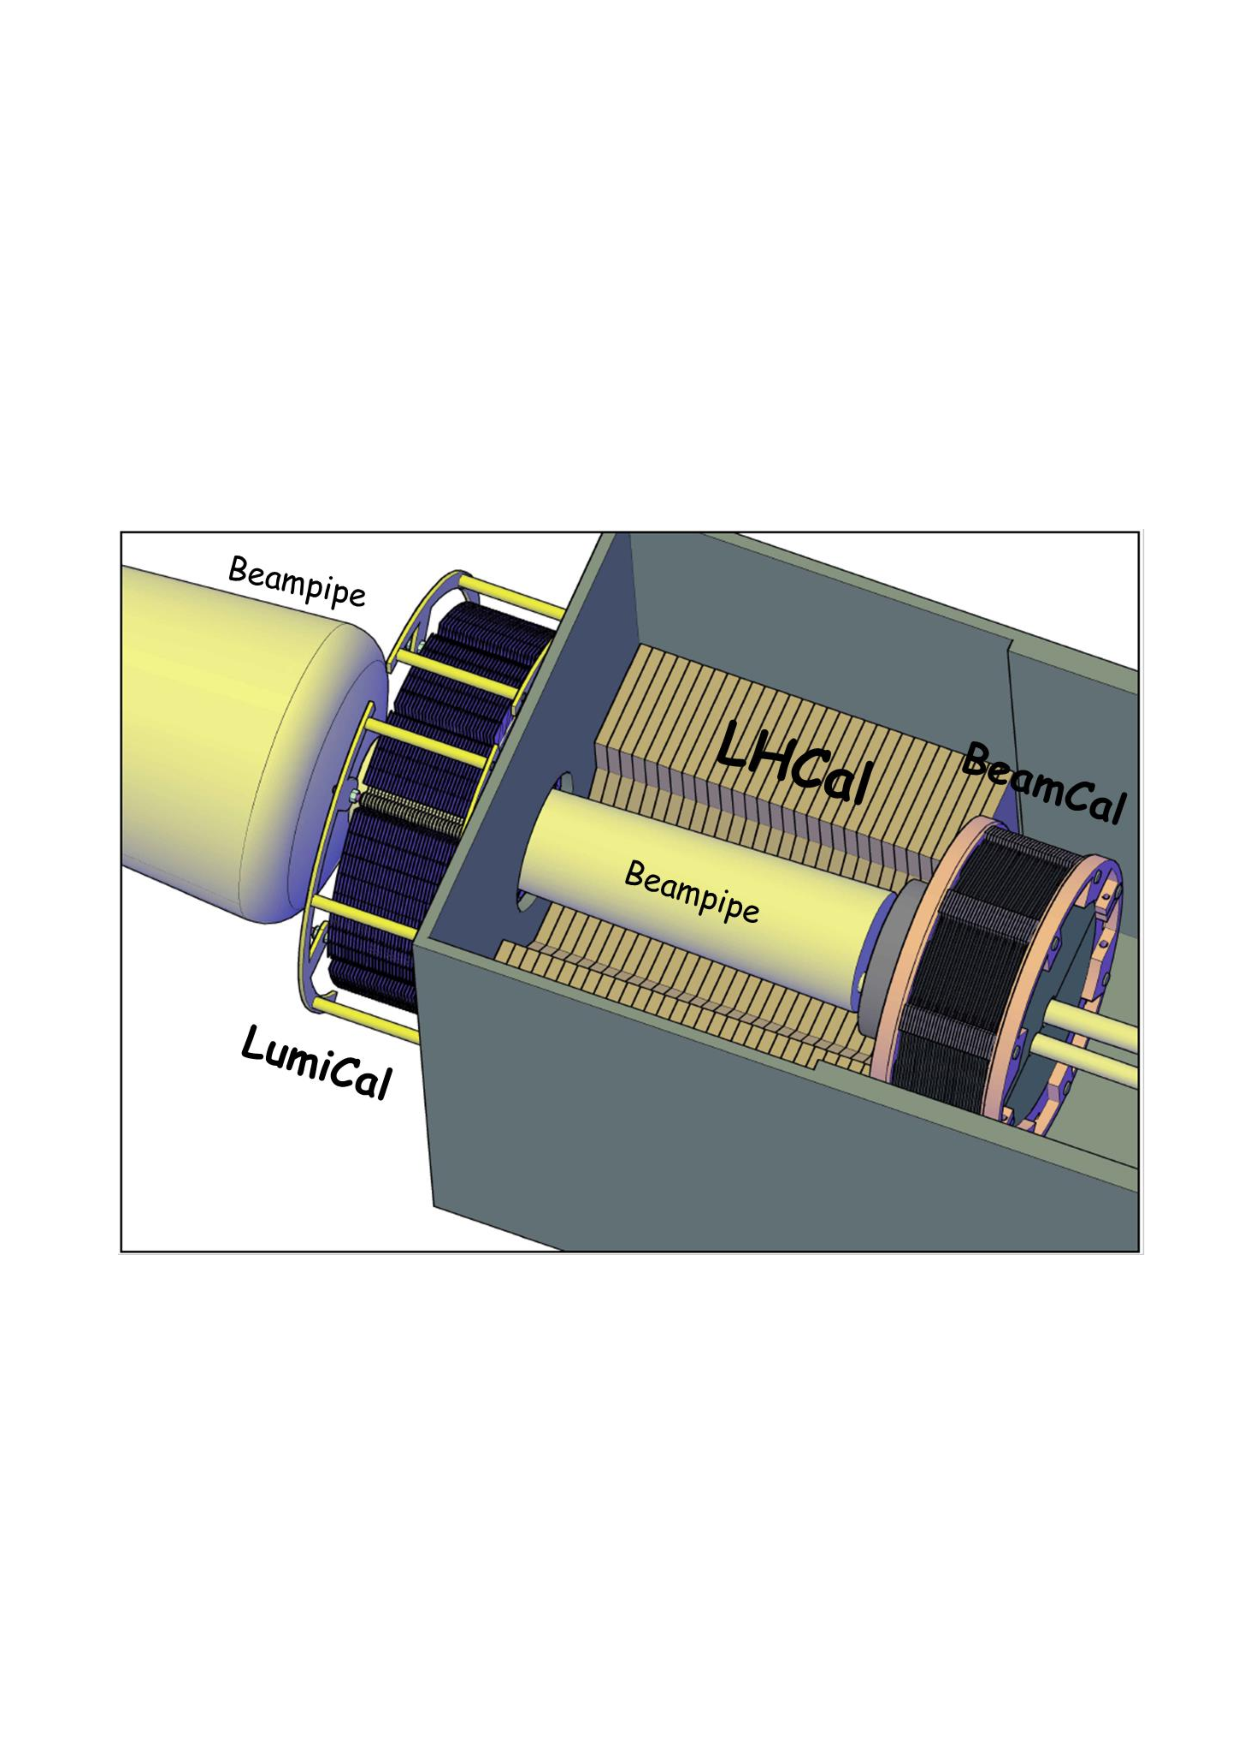
\includegraphics[width=0.45\hsize]{Integration/fig/VFS_Design.pdf}
        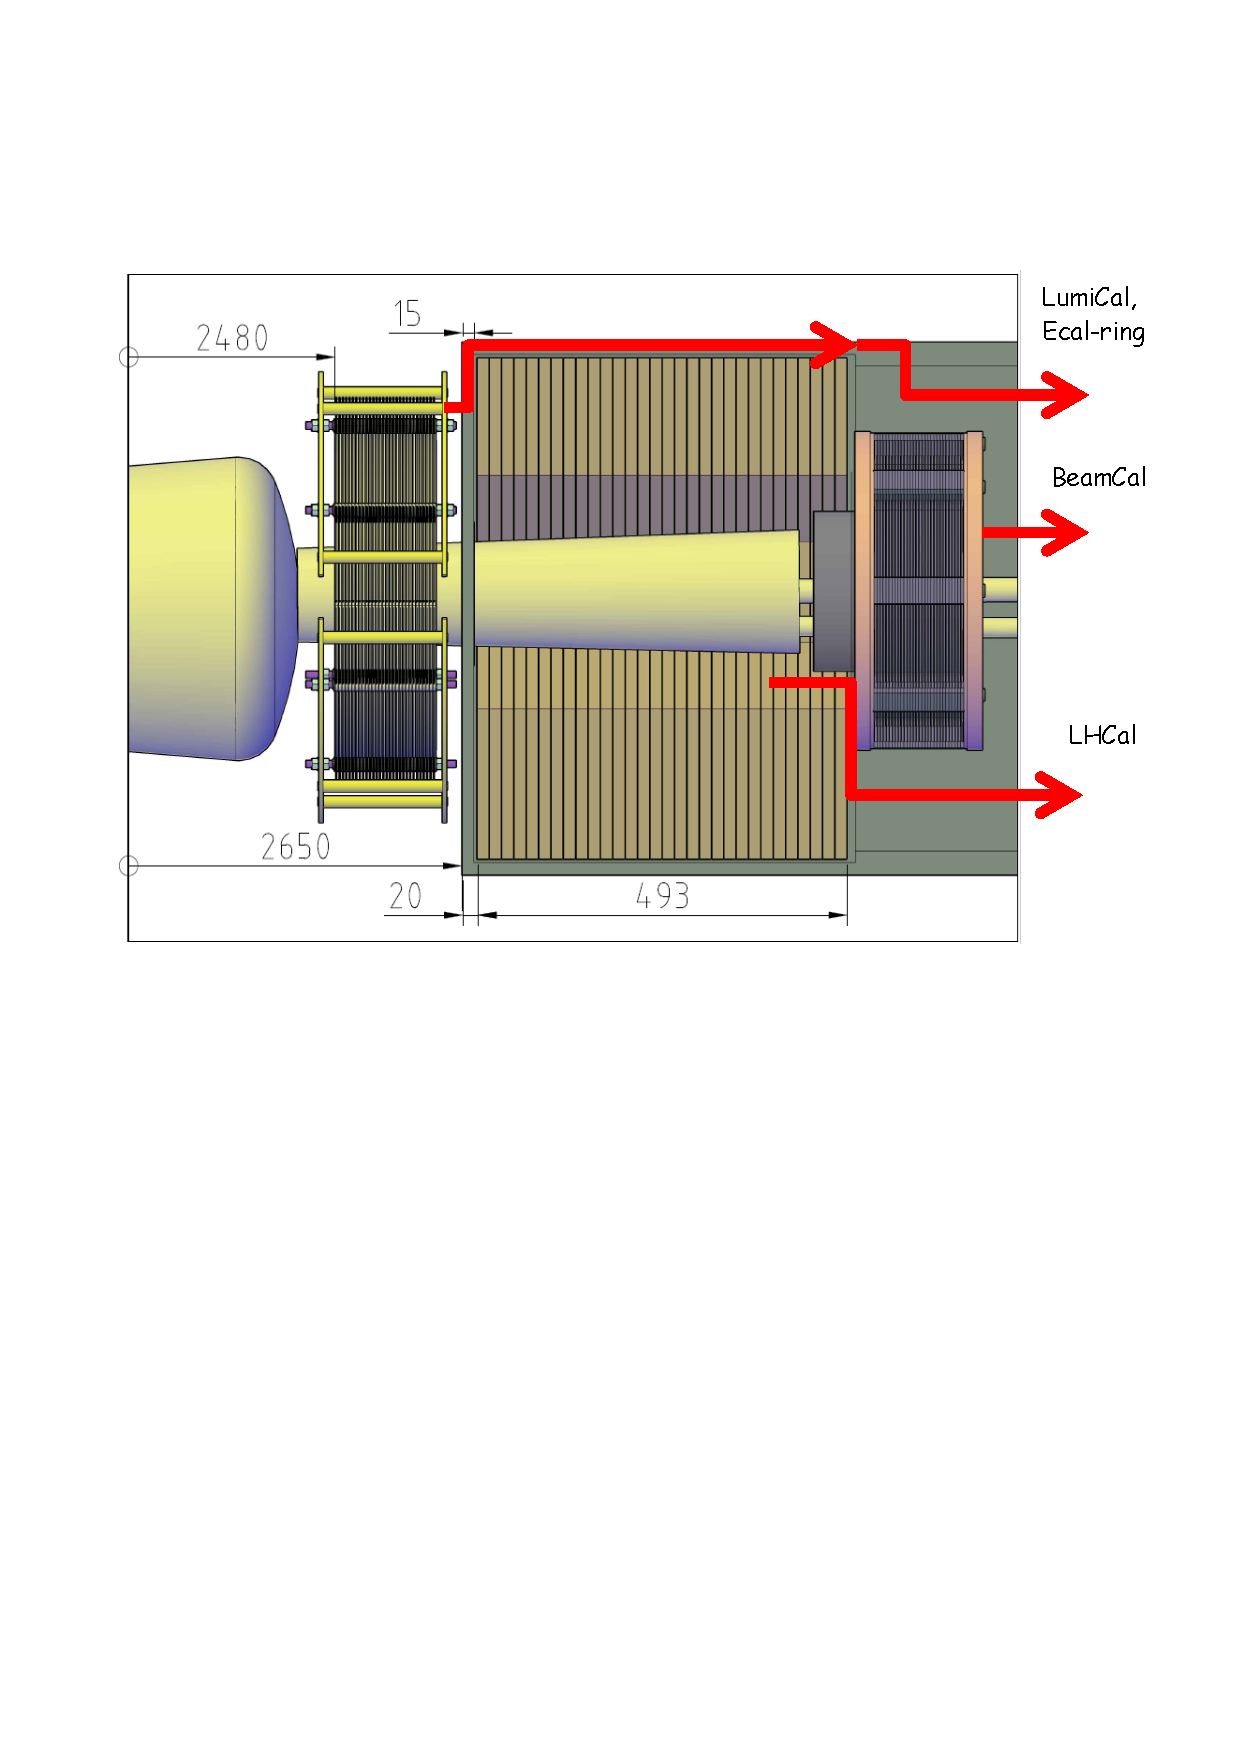
\includegraphics[width=0.45\hsize]{Integration/fig/VFS_Services.pdf}
    \caption{Design of the very forward systems with indication of service and cable paths~\cite{ild:bib:VFS_ICD}.}
    \label{ILD:fig:vfs_integration}
\end{figure}
\section{Data acquisition}
%\writer{Matthew Wing, Taikan Suehara}{2}

The ILD data acquisition takes advantage of the relatively low rate of relevant physics $e^+e^-$ interactions (O(0.1 hadronic evt)/BX) and of the long idle periods between bunch trains (chapter 3) to provide a triggerless readout of the detector. The subdetector data of all BXs of a given bunch train are collected before the next bunch train and processed offline as a single data set for identification, bunch tagging and reconstruction of the individual interactions. 


\subsection{DAQ architecture}

The overall organisation of the DAQ system is summarized in Figure~\ref{fig:integration:DAQ_architecture}. 

\begin{figure}[t!]
\centering
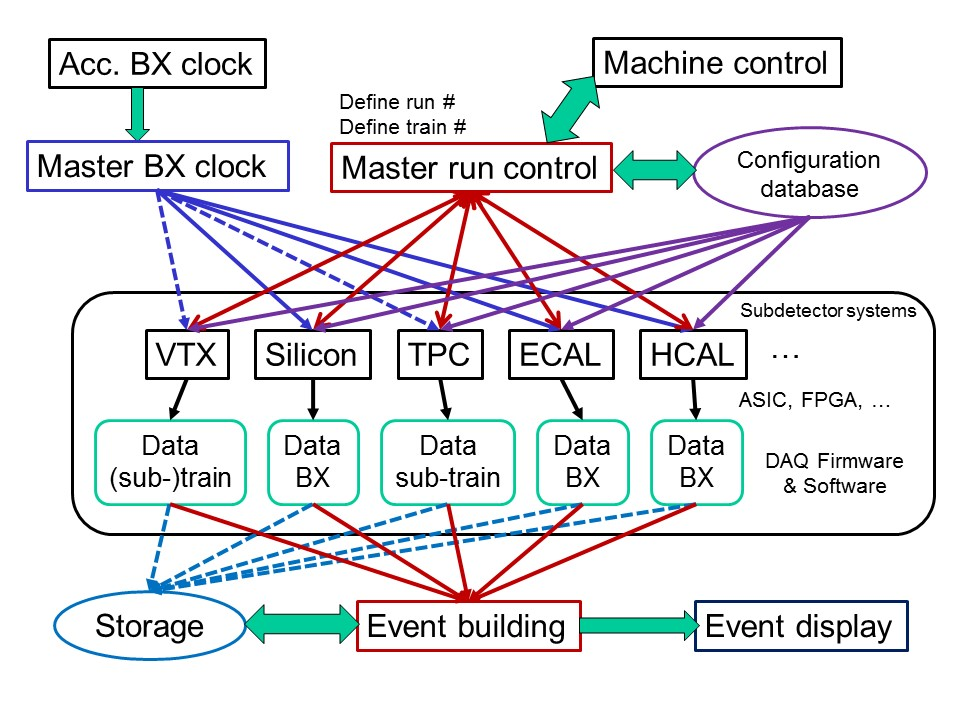
\includegraphics[width=0.75\hsize]{Integration/fig/DAQ_architecture.jpg}
\caption{\label{fig:integration:DAQ_architecture}Global architecture of the ILD data acquisition system.}
\end{figure}

The processing of subdetector data is first performed locally with a high parallelism within FPGA and ASIC boards which each typically treat O(100) subdetector channels. The individual data are zero-suppressed, amplified, time stamped and digitised, depending on the subdetector, and stored in local pipelines dimensioned adequately for a full bunch train. The "event building" is performed between bunch trains by gathering all subdetector data of a given bunch train into a single bunch train data set. The bunch train data sets are stored locally on the IP Campus (section 6.1) and transferred to an offline computing farm which may be located on the main campus. In the farm each bunch train data set is processed individually by one processor in order to identify individual events, tag their bunch crossings and perform calibration and reconstruction. This scheme caters for the different time resolutions of the subdetectors, which range from individual bunch tagging as done e.g. in the calorimeters, to a full train integration time as in the TPC.

One critical component of the system is the clock distribution to the subdetector front-ends: this has to be done on the overall ILD detector with a precision better than 10 ps to enable time-of-flight measurements. On the other hand the overall data flow requirements are moderate. They have not changed significantly compared to the estimates reported in~\cite{ild:bib:ilddbd}, and correspond to a raw data rate of O(100MB)/train for a storage data size of O(10PB)/year. The data flow is dominated by high granularity detectors exposed to high beam background close to the beampipe (VTX and BeamCAL). If needed it could be further reduced by local partial event processing ahead of the event building.

\subsection{DAQ R\&D}

The front-end processing has benefited from the development of subdetector technological prototypes including final readout front-end components as reported in section 5.2. ASIC and FPGA boards with the required ILD specifications are now available for most subdetectors.

A number of common DAQ aspects relevant for the final ILD central DAQ have been developed \cite{ild:bib:AIDADAQ} within the AIDA-2020 programme. They include both hardware and software components which have been used for different detectors or combinations of detectors in beam tests involving not only ILD prototypes but also detectors developed for the HL-LHC. 

The core hardware component of the central DAQ system, the Trigger Logic Unit (TLU), provides a common interface for synchronisation and control of subdetectors. A new TLU has been developed to distribute signals to multiple detectors in beam tests. The AIDA-2020 TLU (Figure~\ref{fig:integration:DAQ_TLU}) has been extended over the previous version to be able to synchronise detectors with differing trigger and readout schemes, such as the CALICE calorimeters, pixel detectors and tracking devices, as well as to be able to operate at a higher particle flux. Therefore, data from different detectors corresponding to the same particle in a test beam can be combined. The TLU is used extensively in test-beam facilities at CERN and DESY and will continue to do so thereby serving the needs of many detectors also beyond ILC R\&D. 

\begin{figure}[t!]
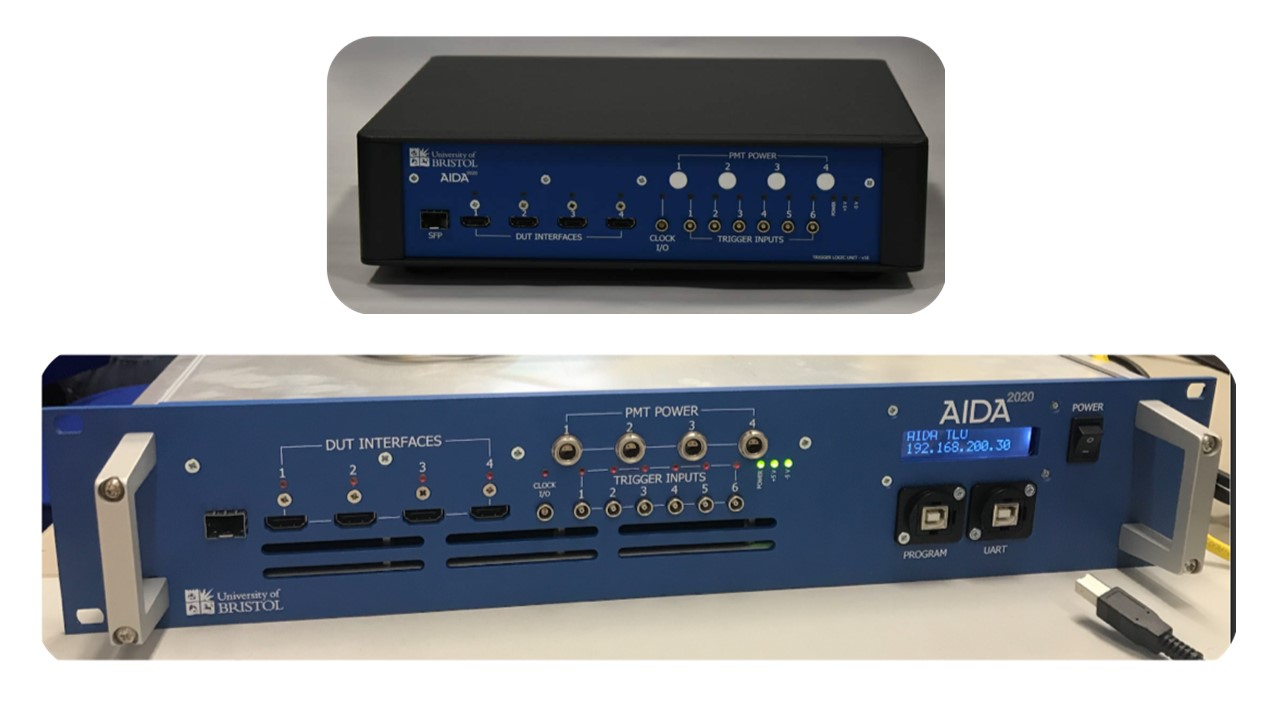
\includegraphics[width=1.0\hsize]{Integration/fig/DAQ_TLU.jpg}
\caption{\label{fig:integration:DAQ_TLU}The AIDA-2020 newly developed Trigger Logic Unit. Top: table top enclosure. Bottom: 19-inch rack-mounted enclosure. The two enclosures have identical inner components and provide the same functionalities.}
\end{figure}

Within AIDA-2020 DAQ software packages have also been developed for both data collection and monitoring. The EUDAQ2 software is an extension of the EUDAQ software developed for the EUDET pixel beam telescope. It supports detectors with different trigger schemes and different readout speeds, enabling combined beam tests of very different detectors to be performed. The software has been tested and used in several beam tests so far, notably for the AHCAL (also in conjunction with the CMS HGCAL), and for tracker modules of the ATLAS upgrade.  The TLU is also fully integrated into the EUDAQ2 framework. The monitoring software, DQM4HEP, originally developed for the SDHCAL, has been used for data quality monitoring and slow control monitoring. This software is a generic development which has extendibility built in and so can be used to monitor data from any detector in any format. It has already been successfully used by the AHCAL+beam telescope and SDHCAL+SiECAL combined beam tests. 

These DAQ developments have allowed multiple detectors to be more easily integrated, sparing time for understanding technical aspects of the detector technologies and the physics performances.  Further detector developments will also benefit from this. The work also informs our understanding of integration and DAQ issues for the final ILD.


\section{Mechanical structure studies}
%\writer{Felix Sefkow, Henri Videau, Karsten Buesser, Roman Poeschl, Toshiaki Tauchi}{3}
\label{ild:sec:mechanical_structures}

The mechanical behaviour of the ILD components is crucial in two respects. On the one hand, the high-precision and hermeticity of the detector requires a precise relative adjustment of subdetector components within each other, with tight tolerances at the interfaces and boundaries. These aspects were studied by simulating static deformations of the components under gravity and other constraints. On the other hand large devices in Japan must obey strict rules as regards their behaviour in case of seismic events (see section~\ref{ild:sec:earthquake}). This was investigated by modelling the dynamic behaviour of components, including the computation of their "eigen modes" and their reaction to reference earthquake parameters from the foreseen ILC Kitakami site. Most of the attention has up to now been given to the calorimeter mechanical structure which governs the global stiffness of the ILD detector inside the coil. %Some evaluations have also started for other subdetectors such as the TPC.

%\subsection{Calorimeter structure}

As mentioned in section~\ref{ild:sec:hcal} two options of the hadronic calorimeter, so-called "Videau" and "TESLA", are under consideration. In both cases, the electromagnetic modules are fixed to the inner plates of the hadronic wheels with two rails parallel to the z direction. Two critical aspects are of particular importance for the calorimeters: the respect of the tolerances of the thin azimutal clearance (2.5mm) between the electromagnetic modules, to avoid mutual contact and possible damage of the modules, and the flatness of the hadronic absorber plates which define the gaps in which the sensitive layers are introduced. The latter is particularly important for the SDHCAL instrumentation option since RPC's require a high level of flatness. Both Videau and TESLA mechanical options have been simulated in detail and the results provide input for further optimization of the layouts.

\subparagraph{\textbf{Videau simulations:}} The static behaviour of a full Videau calorimeter wheel was simulated with a shell model. In order to save computing time, the electromagnetic modules were approximated by a 3D solid model. This simplification was validated separately by a comparison to a single module shell model simulation. The results are shown in Figure~\ref{fig:integration:Videau_deformations}: the hadronic structure turns out to be very stiff with largest deformations of a fraction of a mm. This is due to the vertical flanges of the Videau modules which strongly rigidify the overall structure. The electromagnetic modules are also only slightly distorted: the largest deformation stays below 1mm and the azimutal clearance between modules is reduced to 2.3 mm in the worst case, well within the required tolerances. 

One advantage of the Videau layout is to avoid a projective dead zone at a polar angle of $90^0$, but the number of dead zones in z is 4 for the baseline number of 5 wheels. One question is whether one could reduce this number of dead zones by reducing the number of wheels to 3. Mechanical simulations show that for 3 wheels it is possible to keep deformations at the boundary between the electromagnetic modules within specifications, provided the inner hadronic absorber plate thickness is slightly increased.

First dynamic simulations of the Videau structure were also performed with the computation of eigen modes. They show that the overall calorimeter barrel behaves as a rigid structure under oscillating accelerations, with little variation of the z distance between the wheels. 


\begin{figure}[t!]
\centering
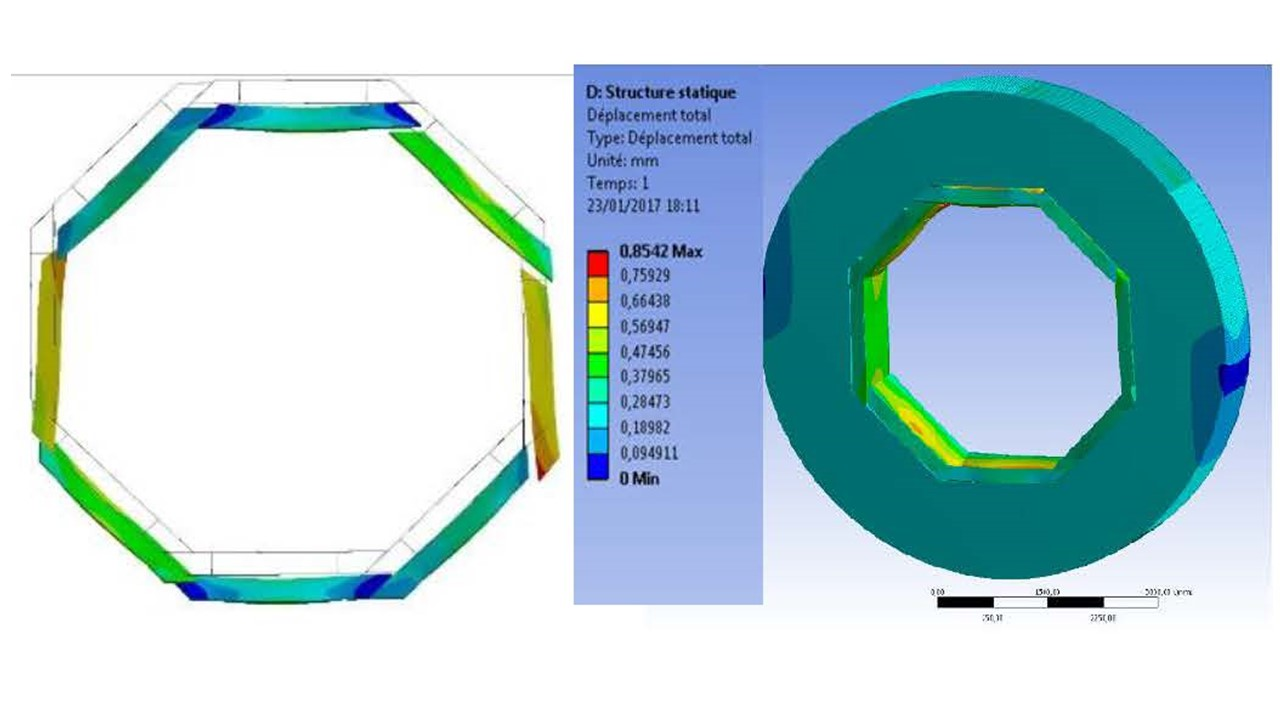
\includegraphics[width=1.0\hsize]{Integration/fig/Videau_deformations.jpg}
\caption{\label{fig:integration:Videau_deformations}Static deformations of the calorimeter "Videau" structure (right, in mm) and zoom on the electromagnetic modules displacements with a magnification factor of 750 (left).}
\end{figure}

\subparagraph{\textbf{TESLA simulations:}} 

In the ILD DBD the TESLA mechanical layout was initiall designed with corners at $0^{o}$, $45^{o}$, $90^{o}$ etc. in azimuth, which corresponded to the optimal configuration as regards mechanical stiffness. In order to facilitate the silicon sensor tiling of the ECAL endcap, the structure has since then been rotated by $22.5^{o}$. Since there are no vertical disks, the behaviour of the structure now resembles that of a Roman arc. 

The mechanical behaviour of the barrel structure with the new orientation has been simulated with shell and 3D models. The simulations showed deformations of up to 5~mm, requiring actions to reduce them. A minimised number of 10~mm wide additional spacers have been introduced between absorber plates in critical points -- near the fixtures of the ECAL and near the supports from the cryostat -- (Figure~\ref{fig:integration:Tesla_deformations} left), resulting in static deformations of less than 2~mm everywhere (Figure~\ref{fig:integration:Tesla_deformations} right). 

\begin{figure}[t!]
\centering
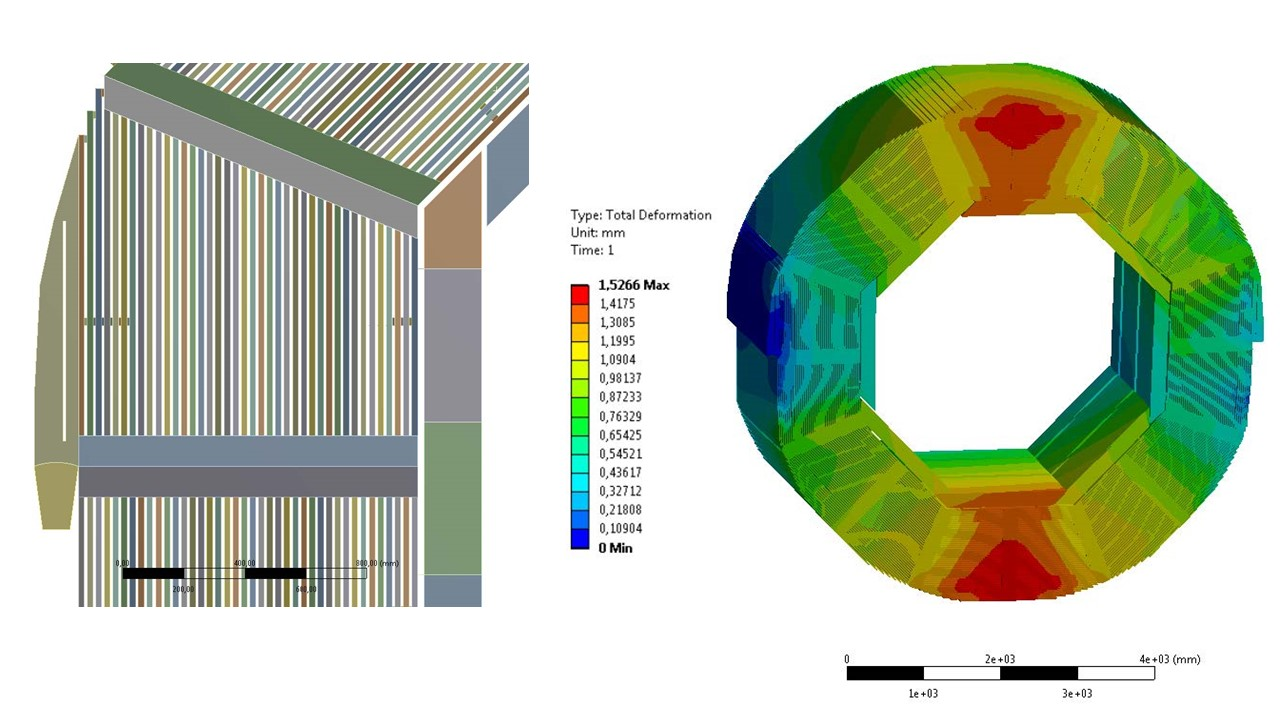
\includegraphics[width=1.0\hsize]{Integration/fig/Tesla_studies.jpg}
\caption{\label{fig:integration:Tesla_deformations}Zoom on the consolidation of the TESLA structure with spacers (left) and resulting static deformations of the structure (right).}
\end{figure}

The 3D model has also been used to obtain the first 200 vibration eigen modes. However, calculating the response of the system to an external excitation exceeds computational limitations and requires more advanced methods. 
The so-called component mode synthesis (CMS) method has been used, in which the detailed sub-structure of calorimeter modules is replaced by blocks which however preserve the overall mechanical behaviour of the module at specially configured boundaries. 
A simplified AHCAL model has been used to validate this model against a full 3D simulation up to the response to frequency sweeps and to real Japanese Earth quake data. 
The application of this model to the re-optimised AHCAL structure is in progress. 

%\subparagraph{\textbf{Simulations cross checks:}} 

%The detailed simulation models of the Videau and TESLA structures have been shared between LLR and DESY in order to allow mutual cross-checks of the results in the future. 

%\subsection{Other subdetectors}

%\textit{If available, results on the mechanical behaviour of other subdetectors (e.g. TPC) are also welcome.}

\vspace{2cm}

e\section{Coil and yoke studies}
%\writer{Karsten Buesser, Uwe Schneekloth}{3}

A conceptual design of the ILD solenoid, the yoke and the cryostat had been developed for the ILD DBD, c.f.~\cite{ild:bib:Magnet_Note, ild:bib:Cryostat_Note}. Recently, studies have been done to optimise the engineering design of the magnet, to study the magnetic properties of the large and small ILD detector models, and to explore possible cost reductions.

\subsection{Magnet Engineering Studies}
A common study by KEK, Toshiba and Hitachi has been started toebeteer understand the engineering challenges in the design and manufacturing of the ILD solenoid coil and the Anti-DID. Figure~\ref{ILD:fig:solenoid_manufacturing} shows a conceptual design of the manufacturing process. While the three solenoid modules and the Anti-DID coils would be fabricated in industry, transportation boundary conditions require the assembly of the complete magnet on or close to the final detector site.
\begin{figure}[h!]
    \centering
    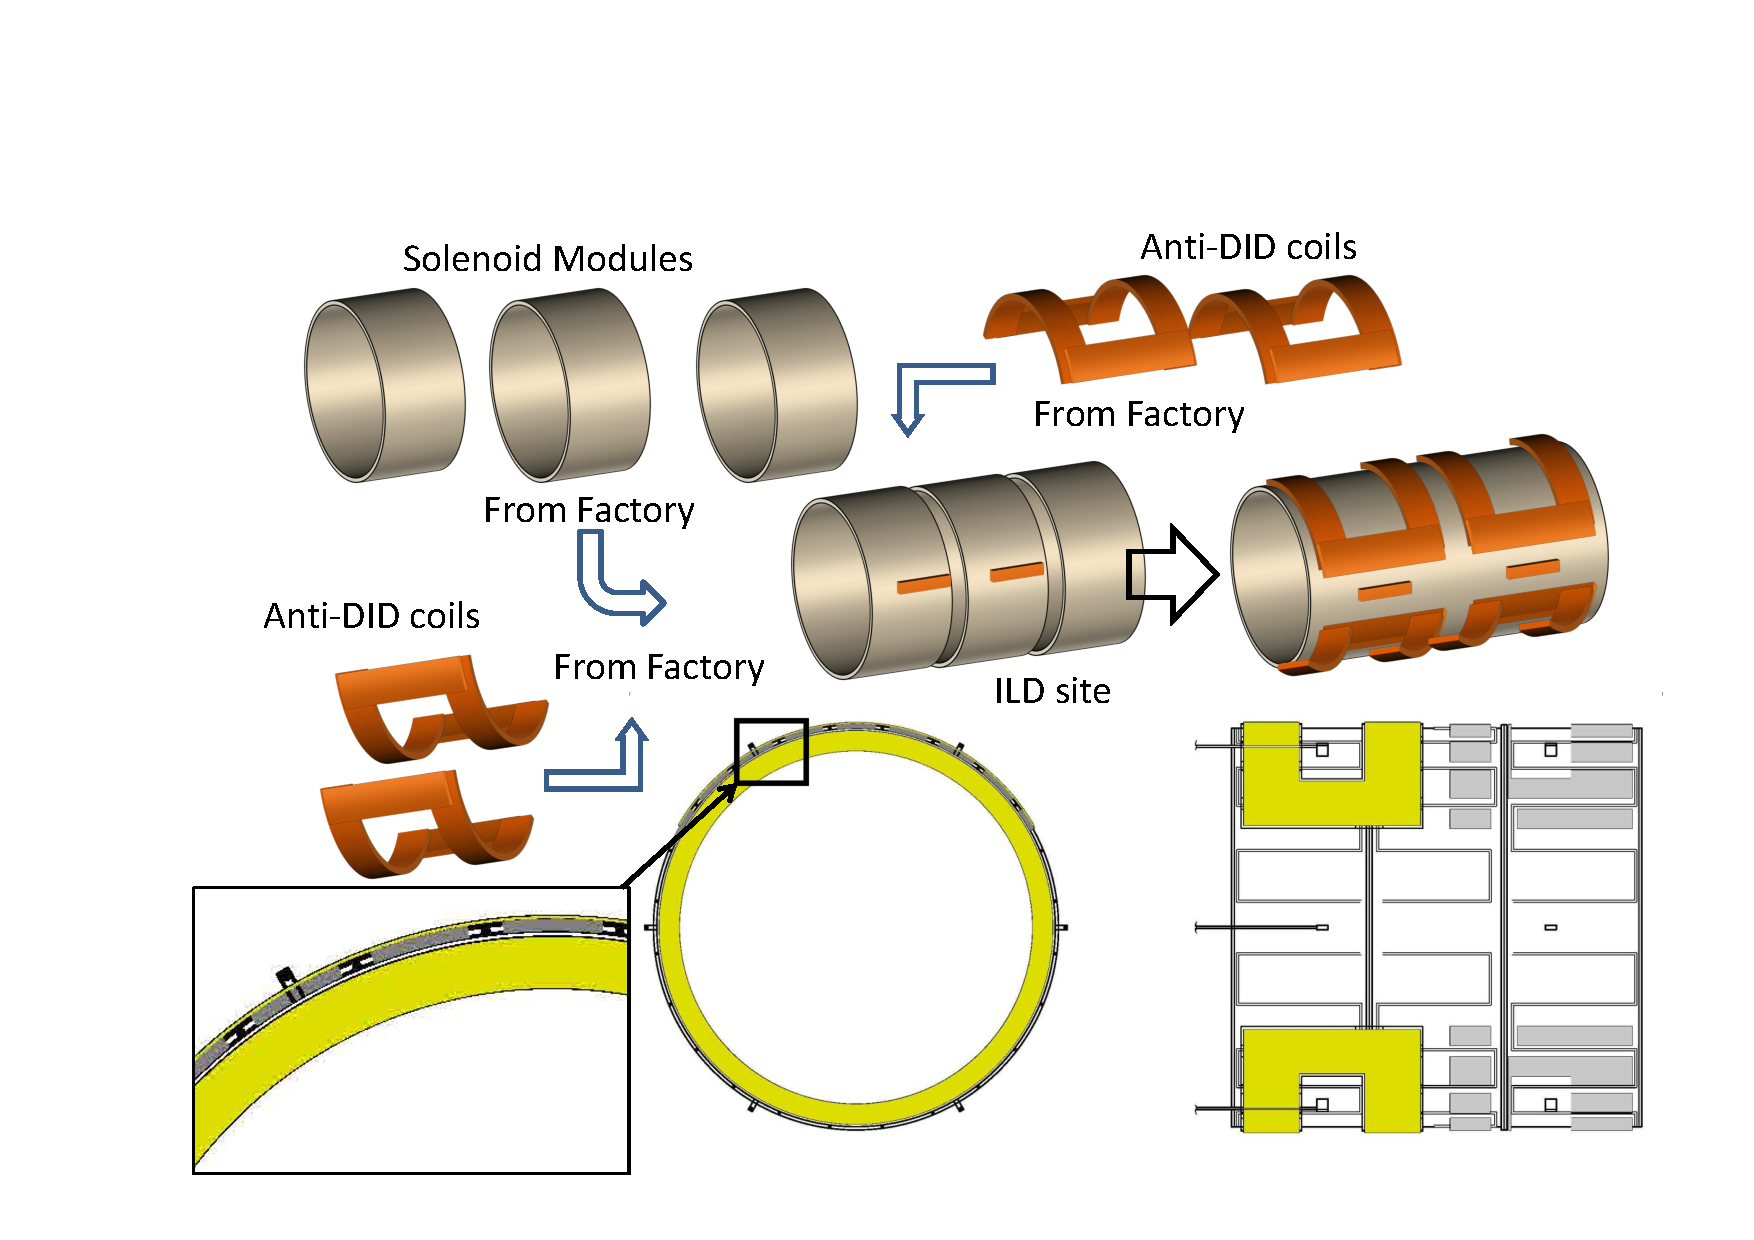
\includegraphics[width=0.8\hsize]{Integration/fig/Solenoid_Manufacturing.pdf}
    \caption{Conceptual manufacturing process of the ILD solenoid and the Anti-DID coils~\cite{ild:bib:Solenoid_Manufacturing}.}
    \label{ILD:fig:solenoid_manufacturing}
\end{figure}
A case study by Toshiba concluded that the main solenoid modules can be transported on street with the use of a specialised Jumbo Carrier while the modules of the Anti-DID would fit on a flatbed trailer~(figure~\ref{ILD:fig:magnet_transport}).
\begin{figure}[h!]
    \centering
    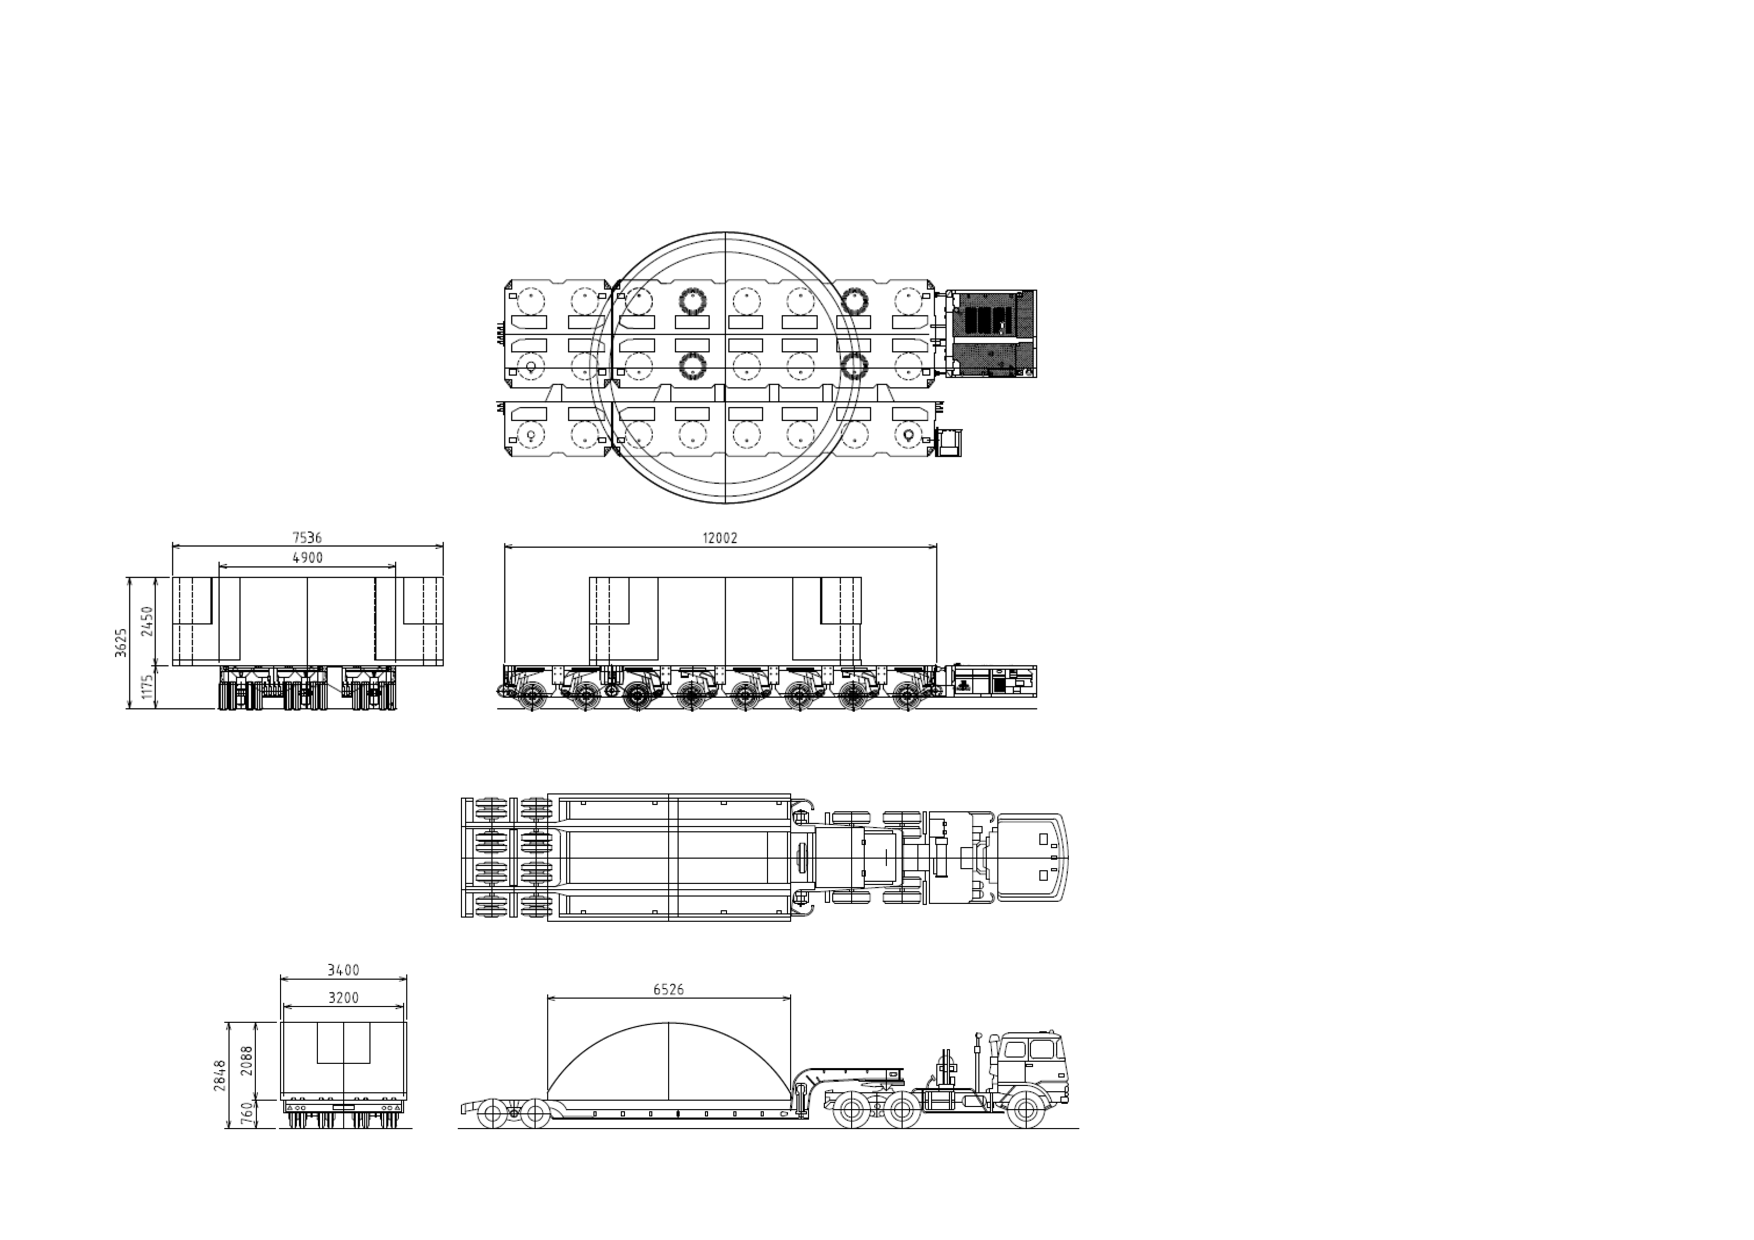
\includegraphics[width=0.8\hsize]{Integration/fig/Magnet_Transport.pdf}
    \caption{While a solenoid module requires transportation by a specialised Jumbo Carrier (top), the Anti-DID modules would fit on a low flatbed trailer (bottom)~\cite{ild:bib:Solenoid_Manufacturing}}
    \label{ILD:fig:magnet_transport}
\end{figure}

The so-called "Anti-DID" coil has been proposed to add a small additional dipole field to the solenoid for better suppression of backgrounds~(c.f. section~\ref{ild:sec:beam_backgrounds} and \cite{ild:bib:anti-did}). Figure~\ref{ILD:fig:anti_did_design} shows a conceptual design of the Anti-DID coils and the resulting simulated dipole field with a maximum value of 0.036~T. Splitting the Anti-DID coils in four makes construction at the manufacturer and transport to the ILC site easier (c.f.~figure~\ref{ILD:fig:magnet_transport}).

\begin{figure}[h!]
%\begin{center}
\begin{subfigure}{0.49\hsize} \includegraphics[width=\textwidth]{Integration/fig/Anti-DID.png}
\caption{ \label{ild:fig:anti_did_mechanics}}
 \end{subfigure}
%\hspace{0.03\textwidth}
\begin{subfigure}{0.49\hsize} \includegraphics[width=\textwidth]{Integration/fig/Anti-DID_Field.pdf}
\caption{  \label{ild:fig:anti-did-field}}
 \end{subfigure}
%\end{center}
\caption{Conceptual design study of the Anti-DID coils (a) and simulated Anti-DID field (b)~\cite{ild:bib:anti-did-design}}
\label{ILD:fig:anti_did_design}
\end{figure}

\subsection{Field Optimisation Studies}

The coil and yoke system should provide at the same time a high magnetic field in the central region and low stray field on the outside of the detector. The nominal fields for the large (small) ILD detector model are 3.5T (4T). To allow for safety margins and possible extensions to higher field values, the coil design has been developed to reach 0.5T more in each case. Figure~\ref{ILD:fig:magnet_nominal} therefore shows the field map and the field distribution for the large ILD detector model and a maximum field of 4T. The corresponding distributions for the small ILD detector model are shown in figure~\ref{ILD:fig:magnet_small}. The field maps are the result of 3D magnetic field simulations. They are implemented in the simulation tools of the detector (chapter 7) to allow for reconstruction with maximum realism when this is required by specific studies such as beam background effects (section 6.5). 

\begin{figure}[t]
\begin{center}
\begin{subfigure}{0.9\hsize} \includegraphics[width=\textwidth]{Integration/fig/field_nominal_4.png}
\caption{ \label{ild:fig:magnet_nominal_map}}
 \end{subfigure}
\hspace{0.03\textwidth}
\begin{subfigure}{0.9\hsize} \includegraphics[width=\textwidth]{Integration/fig/field_nominal_4_plot.png}
\caption{  \label{ild:fig:magnet_nominal_field}}
 \end{subfigure}
\end{center}
\caption{Field map of the ILD solenoid for the large ILD model with a maximum field of 4~T (a) and field distribution along the detector axis (b)~\cite{ild:bib:Magnet_Simulations}}
\label{ILD:fig:magnet_nominal}
\end{figure}

\begin{figure}[t]
\begin{center}
\begin{subfigure}{0.9\hsize} \includegraphics[width=\textwidth]{Integration/fig/field_small_4_5.png}
\caption{ \label{ild:fig:magnet_small_map}}
 \end{subfigure}
\hspace{0.03\textwidth}
\begin{subfigure}{0.9\hsize} \includegraphics[width=\textwidth, height = 6cm]{Integration/fig/field_small_4_5_plot.png}
\caption{  \label{ild:fig:magnet_small_field}}
 \end{subfigure}
\end{center}
\caption{Field map of the ILD solenoid for the small ILD model with a maximum field of 4.5~T (a) and field distribution along the detector axis (b)~\cite{ild:bib:Magnet_Simulations}}
\label{ILD:fig:magnet_small}
\end{figure}


The ILD detector is expected to share its experimental environment with another detector, e.g. SiD, in a push-pull scenario. This model of operations assumes that each detector can run its magnetic field while still allowing the other detector crew to work on their detector with the use of standard iron-based tools. Therefore a limit on the maximum magnetic stray fields has been agreed upon at a maximum of 5~mT at a distance of 15~m from the detector axis~\cite{Parker:2009zz}. This requirement is the main driver for the thickness of the iron yoke of ILD. Figures~\ref{ILD:fig:magnet_nominal_stray} and \ref{ILD:fig:magnet_small_stray} show the simulated stray fields for the large and the small detector model at 4~T and 4.5~T maximum central field.
\begin{figure}[t]
\begin{center}
\begin{subfigure}{0.9\hsize} \includegraphics[width=\textwidth]{Integration/fig/strayfield_nominal_4.png}
\caption{ \label{ild:fig:magnet_nominal_stray_map}}
 \end{subfigure}
\hspace{0.03\textwidth}
\begin{subfigure}{0.9\hsize} \includegraphics[width=\textwidth]{Integration/fig/strayfield_nominal_4_plot.png}
\caption{  \label{ild:fig:magnet_nominal_stray_field}}
 \end{subfigure}
\end{center}
\caption{Map of the ILD solenoid strayfield for the large ILD model with a maximum central field of 4~T (a) and field distribution at a distance of 15~m parallel to the detector axis (b)~\cite{ild:bib:Magnet_Simulations}.}
\label{ILD:fig:magnet_nominal_stray}
\end{figure}

\begin{figure}[h!]
\begin{center}
\begin{subfigure}{0.9\hsize} \includegraphics[width=\textwidth]{Integration/fig/strayfield_small_4_5.png}
\caption{ \label{ild:fig:magnet_small_stray_map}}
 \end{subfigure}
\hspace{0.03\textwidth}
\begin{subfigure}{0.9\hsize} \includegraphics[width=\textwidth, height =6cm]{Integration/fig/strayfield_small_4_5_plot.png}
\caption{  \label{ild:fig:magnet_small_stray_field}}
 \end{subfigure}
\end{center}
\caption{Field map of the ILD solenoid for the small ILD model with a maximum field of 4.5~T (top) and field distribution at a distance of 15~m parallel to the detector axis (bottom)~\cite{ild:bib:Magnet_Simulations}.}
\label{ILD:fig:magnet_small_stray}
\end{figure}

Simulations have been done with different codes and the results are very consistent with an average value for the large detector of 5.6$\pm$0.6~mT for the maximum stray field at 15~m~\cite{ild:bib:Magnet_Simulations}. The stray fields for the small detector model are very similar. 

The stringent limits on the stray fields are a cost driver for ILC as they drive the thickness of the iron return yoke. If the thickness would be reduced by 60~cm, the maximum stray fields at 15~m would increase to 9.3$\pm$0.8~mT but at the same time reduce the cost for the yoke by about 20\% for the large ILD detector model~\cite{ild:bib:Magnet_Simulations}.

A cost reduction of in total $\approx$50\% can be reached if the iron yoke is reduced further to a thickness of 2.04~m (including gaps). The stray fields at 1~m distance from the outside of the yoke would be at the level of 100~mT which is acceptable for the operation of magnetically sensitive equipment and which is well below limits given by human safety regulations. The far stray fields in direction of the other detector need to be shielded in that case, e.g. by using a magnetic shielding wall. Figure~\ref{ILD:fig:magnet_wall} shows the simulation of the large ILD detector model magnetic fields with a reduced yoke and a shielding wall.

Though this concept looks attractive, further studies are required. The shielding wall needs to be mobile and has to follow the push-pull movements. An engineering solution needs to be developed. Another problem is the radiation shielding. In the present design, the thick iron yoke serves as a radiation shield and allows for access to the outer side of the detector while the ILC delivers beams to the interaction region~\cite{ild:bib:Radiation_Hall}. A reduced yoke might be too thin to serve for this purpose alone and additional radiation shielding, e.g. made from concrete, might need to be added. 
\begin{figure}[htb]
    \centering
    \includegraphics[width=0.8\hsize]{Integration/fig/magnet_wall.png}
    \caption{Field map of the ILD solenoid for the large ILD model with a iron shielding wall towards the direction of the other detector in the experimental hall~\cite{ild:bib:Magnet_Simulations}.}
    \label{ILD:fig:magnet_wall}
\end{figure}



\section{\label{sec:beam:background} Beam background studies}
%\writer{Daniel Jeans, Yan Benhammou, Sergej Schuwalow, Claude Vallee}{2}
\label{ild:sec:beam_backgrounds}
The ILD detector response is affected by three main sources of beam-related background: beamstrahlung emitted at the crossing point of the electron and positron bunches, halo muons produced upstream of the detector along the beamline, and low energy neutrons back-scattered from the beam dumps. Their impact on the detector occupancies has been quantified and possible mitigation investigated\cite{ild:bib:Machine_Backgrounds,ild:bib:schuetz_thesis}. Results are similar for both options of the ILD detector and are shown here for the large version.

\subsection{Beamstrahlung}

Beamstrahlung photons are radiated from the ILC beam particles in the interaction with the electromagnetic fields of the strongly focused oncoming bunches. These photons can convert to $e^+e^-$ pairs with a broad energy spectrum. Most of the low-energy pairs are confined close to the z axis by the solenoid magnetic field but, due to the crossing angle between the colliding beams, a significant fraction hit the very forward detectors near the incoming and outgoing beam pipes. The central detectors are also affected, both directly by the $e^+e^-$ pairs, and indirectly through back-scattering of low-energy particles from the forward detectors. It was proposed to mitigate these effects by the addition of a small dipole field to the main solenoidal field. This so-called "anti-DID" field can be tuned to guide a large fraction of the  $e^+e^-$ pairs into the outgoing beampipe. 

These effects have been quantified for the updated 250 GeV ILC conditions (ILC250, see Section~\ref{ild:sec:ilc}), using a full simulation of the beamstrahlung particle production and of their tracking within ILD~\cite{ild:bib:Machine_Backgrounds}. Special care has been taken to ensure stable results by adapting the GEANT4 tracking parameters to low energy particles. A realistic field map of both solenoid and anti-DID fields has been used. The response of the most affected detector, the BeamCAL, is shown in Figure~\ref{fig:integration:beamcal} with and without anti-DID. A positive effect of the anti-DID is clearly visible: when the anti-DID field is applied, the particle distribution is more symmetric around the central beampipe, and the overall energy deposition in BeamCAL is reduced by about 30\%.

\begin{figure}[t!]
\begin{subfigure}{0.48\textwidth}
\includegraphics[width=1.0\hsize]{Integration/fig/BG_beamcal_a.jpg}
\caption{}
\end{subfigure}
\begin{subfigure}{0.48\textwidth}
\includegraphics[width=1.0\hsize]{Integration/fig/BG_beamcal_b.jpg}
\caption{}
\end{subfigure}
\caption{\label{fig:integration:beamcal}Beamstrahlung energy deposition in the BeamCAL without (a) and with (b) anti-DID field for the large ILD version at ILC-250 (arbitrary units). }
\end{figure}

\begin{table}
\begin{center}
\begin{tabular}{ l c c c }
\toprule
LAYER: & hits/BX & hits/BX & hits/BX/$cm^2$ \\
& No anti-DID & anti-DID & anti-DID \\
& mean $\pm$ RMS & mean $\pm$ RMS & mean $\pm$ RMS \\
\midrule
VXD 1: & 1400 $\pm$ 780 & 910 $\pm$ 360 & 6.6 $\pm$ 2.6 \\
VXD 2: & 970 $\pm$ 560  & 540 $\pm$ 210 & 4.0 $\pm$ 1.5 \\
VXD 3: & 150 $\pm$ 80   & 130 $\pm$ 60  & 0.21 $\pm$ 0.10 \\
VXD 4: & 110 $\pm$ 60   & 110 $\pm$ 50  & 0.18 $\pm$ 0.09 \\
VXD 5: & 44 $\pm$ 30    & 40 $\pm$ 26   & 0.04 $\pm$ 0.03 \\
VXD 6: & 39 $\pm$ 27    & 34 $\pm$ 24   & 0.04 $\pm$ 0.03 \\
\midrule
FTD 1: & 42 $\pm$ 30 & 38 $\pm$ 26 & 0.043 $\pm$ 0.030 \\
FTD 2: & 27 $\pm$ 19 & 24 $\pm$ 15 & 0.029 $\pm$ 0.019 \\
FTD 3: & 62 $\pm$ 45 & 40 $\pm$ 27 & 0.014 $\pm$ 0.010 \\
FTD 4: & 42 $\pm$ 33 & 25 $\pm$ 17 & 0.009 $\pm$ 0.007 \\
FTD 5: & 29 $\pm$ 23 & 18 $\pm$ 13 & 0.007 $\pm$ 0.005 \\
FTD 6: & 16 $\pm$ 13 & 9 $\pm$ 7   & 0.004 $\pm$ 0.003 \\
FTD 7: & 10 $\pm$ 8  & 6 $\pm$ 5   & 0.003 $\pm$ 0.003 \\
\midrule
SIT 1: & 51 $\pm$ 37 & 24 $\pm$ 16 & 0.0032 $\pm$ 0.0023 \\
SIT 2: & 49 $\pm$ 36 & 21 $\pm$ 12 & 0.0029 $\pm$ 0.0017 \\
SIT 3: & 77 $\pm$ 56 & 34 $\pm$ 24 & 0.0014 $\pm$ 0.0010 \\
SIT 4: & 71 $\pm$ 54 & 31 $\pm$ 21 & 0.0013 $\pm$ 0.0009 \\
\midrule
SET 1: & 39 $\pm$ 28 & 15 $\pm$ 10 & 0.00003 $\pm$ 0.00002 \\
SET 2: & 46 $\pm$ 36 & 18 $\pm$ 12 & 0.00003 $\pm$ 0.00002 \\
\bottomrule
\end{tabular}
\end{center}
\caption{\label{ild:tab:BGhits}Number of beamstrahlung hits per bunch crossing in the silicon trackers without (left) and with (middle and right) anti-DID field for the large ILD version at ILC250.}
\end{table}



A similar improvement is seen for the central detectors in table~\ref{ild:tab:BGhits}. The most affected are the inner layers of the vertex detector, where the background is equally shared between direct hits rather uniformly distributed, and back-scattered particles showing hot spots in azimuth. Background hits further away from the beampipe are dominated by direct $e^+e^-$ pairs. The anti-DID has little effect on direct $e^+e^-$ hits but helps to suppress back-scattered particles and associated hot spots in the central detectors.
%\textit{Comment also on TPC hits}.

For the small ILD version, the overall beamstrahlung background hit rates are reduced by $\approx$10\%  thanks to better confinement within the beampipe by the higher solenoid field of 4T.

%\textit{Add info on beamstrahlung effects on beamcal reconstruction and on HCAL occupancy near beampipe}

%\begin{figure}[t!]
%\includegraphics[width=0.8\hsize]{Integration/fig/BG_rates.jpg}
%\caption{\label{fig:integration:rates}Number of beamstrahlung hits per bunch crossing in the silicon trackers without (left) and with (right) anti-DID field for the large ILD version at ILC250. \textit{Give rates per $cm^2$ and transform figure into latex table.}}
%\end{figure}

\subsection{Halo muons}

The electrons and positrons of the beam halo produce high-energy penetrating muons parallel to the beam by interacting with beamline components such as collimators. Beam simulations~\cite{Keller:2019aak} predict that a fraction of $10^{-3}$ of the incident beam electrons hit a machine component of the beam delivery system and may therefore produce muons. Five magnetized muon spoilers and one optional larger magnetized muon wall are foreseen to deviate these muons outside the ILC experimental hall. The resulting rate of muons in ILD has been simulated for ILC250 and ILC500. 

\begin{figure}[t!]
\includegraphics[width=1.0\hsize]{Integration/fig/BG_muons.jpg}
\caption{\label{fig:integration:muons}Energy spectrum of muons entering the ILC experimental hall for ILC500, normalised to a full single train of 2625 bunches assuming a beam halo fraction of $10^{-3}$. Red curve: muon filtering with 5 spoilers only; Blue curve: muon filtering with an additional muon wall~\cite{ild:bib:schuetz_thesis}.}
\end{figure}

Figure~\ref{fig:integration:muons} shows the energy spectra of the muons crossing the ILD detector for the two filtering options. The muon wall significantly reduces the flux of the lower energy muons below a few 10 GeV. At ILC500 the rate of halo muons crossing ILD is of the order of 4 (resp. 0.6) muons/BX without (resp. with) the optional muon wall. At ILC250 the corresponding numbers are of the order 1 and 0.03 muons/BX for the two filtering options, respectively.

These halo muons will affect the occupancy of the detector but should be easily identified and subtracted from the physics events using topological and timing information.

\subsection{Backscattered neutrons from beam dumps}

A potential additional source of beam-related background consists in particles back-scattered from the electron and positron beam dumps located 300m from the interaction point in both beam directions. This background is expected to be dominated by low energy neutrons which can propagate over a long distance. Their contribution has been fully simulated with FLUKA in the context of SiD, including a detailed description of the beamline up to the beam dump as well as of the dump system itself~\cite{ild:bib:schuetz_thesis}. The incoming neutron fluxes close to SiD are expected to be the same as for ILD and were interfaced to the ILD detector simulation to estimate their impact in the detector. The simulation was normalised to the dump of one full electron bunch on the +z side of the detector.

The total number of neutrons reaching the ILD detector region is found to be O($10^6$) per electron bunch dump. These neutrons have very low momenta of a few 10 MeV and most of them do not deposit a detectable signal in the detector. Their propagation in ILD was simulated and the map of their stopping points in the detector is shown in Figure~\ref{fig:integration:neutrons}. The results are in line of what is found for SiD~\cite{ild:bib:schuetz_thesis}: most neutrons are absorbed in the external layers of the ILD iron yoke, with a very small fraction reaching the external layers of the very forward calorimeters. Their energy depositions concentrate close to their stopping points: they are very small ($\approx$0.1 MIP on average) and asynchronous with respect to the bunch crossings. No visible signal is seen in the ILD vertex detector and central tracker. This indicates that the neutron background should not be a critical issue within its current state of understanding.

\begin{figure}[t!]
\centering
\begin{subfigure}{0.40\textwidth}
\includegraphics[width=1.0\hsize]{Integration/fig/BG_neutrons_a.jpg}
\caption{}
\end{subfigure}
\begin{subfigure}{0.48\textwidth}
\includegraphics[width=1.0\hsize]{Integration/fig/BG_neutrons_b.jpg}
\caption{}
\end{subfigure}
\caption{\label{fig:integration:neutrons}Map of the stopping points in ILD of neutrons back-scattered from the beamdump: (a) transverse coordinates and (b) longitudinal coordinates. The maps are normalised to the dump of one electron bunch on the +z side of ILD~\cite{ild:bib:schuetz_thesis}.}
\end{figure}



\section{Alignment/ calibration procedures}
\writer{Graham Wilson, Ties Behnke}{1}

There was little progress here since the LOI/DBD. Most of the corresponding text of these documents could be recovered and summarized for the IDR, taking into account the latest considerations about in-situ calibration with particles/collisions and subdetector requirements.

\vspace{2cm}

\section{Earthquake Safety}
\label{ild:sec:earthquake}
Japan is one of most seismically active regions in the world. The proposed site for the ILC in the Kitakami mountains of northern Honshu has been especially selected putting emphasis on benign seismic conditions. Earthquake history has been taken into account as well as recent surveys on active tectonic faults. Nevertheless, earthquakes can occur and need to be taken into account. Figure~\ref{ild:fig:integration:earthquake_map} shows all earthquakes that were detected during 30 days in winter 2018/2019 in northern Honshu. The ILD interaction region is in the region around (39N, 141,5E).

\begin{figure}[h!]
\centering
\includegraphics[width=0.8\hsize]{Integration/fig/earthquake_map.png}

\caption{\label{ild:fig:integration:earthquake_map}Map of northern Honshu with all detected earthquakes between 23rd December 2018 and 23rd January 2019 (30 days)~\cite{ild:bib:hi-net}. The ILC site is indicated by the red ellipse.}
\end{figure}

\subsection{Structural Design}

Emphasis has been put on the design of the ILD detector with respect to earthquake safety in view of operability of the detector as well as disaster prevention. General rules are provided by the ISO3010 standard: "Bases for design of structures -- seismic actions on structures". The ISO standard states two basic principles:
\begin{itemize}
\item The structure should not collapse nor experience other similar forms of structural failure due to severe earthquake ground motions that could occur at the site (ultimate limit state: ULS).
\item The structure should withstand moderate earthquake ground motions which may be expected to occur at the site during the service life of the structure with damage within accepted limits (serviceability limit state: SLS).
\end{itemize}

The design seismic forces on mechanical structures can be determined by taking into account normalised design response spectra, weighted with load factors that take into account the respective state, ULS or SLS, local conditions and structural factors. In addition, required degrees of reliability of the structures can be taken into account.

An acceleration response spectrum for the SLS state at the Kitakami site is shown in Figure~ \ref{ild:fig:integration:earthquake_spectra} for structures with different damping behaviours. In the ULS state, the accelerations are assumed to be larger by about a factor of two. These type of standard spectra serve as input for the structural studies described in section~\ref{ild:sec:mechanical_structures}.
\begin{figure}[t!]
\includegraphics[width=0.8\hsize]{Integration/fig/earthquake_spectra.pdf}
\caption{\label{ild:fig:integration:earthquake_spectra}Standard response spectra for earthquakes in Kitakami (hard soil) for structures with different damping behaviour~\cite{ild:bib:earthquake}. A maximum acceleration of 150~gal (1 gal = 1 cm/s$^2$) for an earthquake with a recurrence frequency of 100~years has been assumed.}
\end{figure}

\subsection{Seismic Isolation}

Seismic isolation could be an attractive solution to mitigate the risk of earthquake induced accidents. Base isolation systems are in use in many cases in seismic active countries like Japan, under buildings, bridges and other critical infrastructure. A recent study~\cite{ild:bib:Seismic_Damping} has explored the possibility to install seismic damping systems underneath the ILD detector, e.g. under the detector platform. Standard isolation systems consist of rubber bearings in combination with oil dampers. Figure~\ref{ild:fig:integration:damping_earthquake} shows that accelerations acting on the ILD detector could be damped by a factor of $\approx$35 in case of a catastrophic earthquake. At the same time, such a system unfortunately increases the displacements of the detector in case of seismic mircrotremors that occur frequently in Japan, also at the Kitakami site~(c.f.~Figure~\ref{ild:fig:integration:earthquake_map}). An extended system that adds a rigid sliding bearing could mitigate the problem. Here, friction keeps the detector coupled to the ground at lower acceleration forces. Figure~\ref{ild:fig:integration:damping_microtremor} shows that no amplification of microtremors happens in that case. At the same time, the damping behaviour in case of major earthquakes is still in the order of a factor of $\approx$22 better than without base isolation~(Figure~\ref{ild:fig:integration:damping_earthquake}). 

\begin{figure}[h!]
\begin{center}
\begin{subfigure}{0.9\hsize} \includegraphics[width=\textwidth]{Integration/fig/Damping_Earthquake.pdf}
 \caption{ \label{ild:fig:integration:damping_earthquake}}
 \end{subfigure}
\hspace{0.03\textwidth}
\begin{subfigure}{0.9\hsize} \includegraphics[width=\textwidth]{Integration/fig/Damping_Microtremor.pdf}
 \caption{  \label{ild:fig:integration:damping_microtremor}}
 \end{subfigure}
\end{center}
\caption{
(a) Simulated accelerations on the ILD detector in case of a catastrophic earthquake without base isolation (top) with an rubber bearing/oil damper system (middle) and with an additional rigid sliding bearing (bottom). Acceleration spectra from the 2011 Tohoku earthquake have been used as a case study for a most severe case~\cite{ild:bib:Seismic_Damping}.
(b) Simulated displacements of the ILD detector in case of microtremors without base isolation (top) with an rubber bearing/oil damper system (middle) and with an additional rigid sliding bearing (bottom) \cite{ild:bib:Seismic_Damping}.
}
\end{figure}


%\begin{figure}[h!]
%\centering
%\includegraphics[width=0.8\hsize]{Integration/fig/Damping_Earthquake.pdf}
%\caption{\label{ild:fig:integration:damping_earthquake}Simulated accelerations on the ILD detector in case of a catastrophic earthquake without base isolation (top) with an rubber bearing/oil damper system (middle) and with an additional rigid sliding bearing (bottom). Acceleration spectra from the 2011 Tohoku earthquake have been used as a case study for a most severe case~\cite{ild:bib:Seismic_Damping}.}
%\end{figure}
%\begin{figure}[h!]
%\centering
%\includegraphics[width=0.8\hsize]{Integration/fig/Damping_Microtremor.pdf}
%\caption{\label{ild:fig:integration:damping_microtremor}Simulated displacements of the ILD detector in case of microtremors without base isolation (top) with an rubber bearing/oil damper system (middle) and with an additional rigid sliding bearing (bottom) \cite{ild:bib:Seismic_Damping}.}
%\end{figure}

A seismic base isolation system underneath the detector platform could therefore mitigate seismic risks for the ILD detector. However, earthquakes could also occur when the detector is still under construction or has been opened and moved partially away from the platform. Systematic risk evaluations and the development of mitigation strategies for the full lifetime of ILD still need to be done.

\section{Technical Documentation}

The technical description of the ILD detector concept comprises specification and design documents as well as 3D engineering models, interface descriptions and drawings. All the documents that form the backbone of the ILD technical documentation are stored in the ILC Engineering Data Management System ILC-EDMS~\cite{ild:bib:edms}. As this powerful system is made for experts and requires appropriate attention, an easy accessible frontend ("EDMSdirect") has been made available. The ILD technical documentation is organised in a Work Breakdown Structure (WBS) that is mapped on a tree browser that can be accessed on the web~\cite{ild:bib:edmsdirect}. Figure~\ref{ild:fig:integration:edmsdirect} shows the tree browser for the ILD technical documentation. All WBS top nodes can be expanded by clicking on them. In the Figure, this has been done for the node "Design Integration".


\begin{figure}[t!]
\centering
\includegraphics[width=0.8\hsize]{Integration/fig/EDMS_direct.png}

\caption{\label{ild:fig:integration:edmsdirect}Part of the treebrowser of the ILD technical documentation Work Breakdown Structure in the ILC Engineering Data Management System. The top level node "Design Integration" is shown expanded.}
\end{figure}

Figure~\ref{ild:fig:integration:edmsdirect_document} shows the document browser that opens for the documents stored in the EDMSdirect system. Shown here is the "Conventions and Rules" document that belongs to the previous mentioned WBS node "Design Integration". A preview of the document is shown in the document browser. The document browser allows for preview of the respective documents as well as downloads of pdf or source files, depending on the authorisation of the users. Documents can be made worldwide visible as well as protected for selected users.

\begin{figure}[h!]
\centering
\includegraphics[width=0.8\hsize]{Integration/fig/EDMS_direct_document.png}

\caption{\label{ild:fig:integration:edmsdirect_document}Example document (here:"ILD Conventions and Rules") in the document browser of EDMSdirect.}
\end{figure}

\subsection{Interface Control Documents}
The technical integration of the ILD detector is based on a set of Interface Control Documents which describe the interfaces of each subdetector to its environment:
\begin{itemize}
    \item Mechanical Interface
    \begin{itemize}
        \item Local coordinate system
        \item Mechanical concept
        \item Critical dimensions
        \item Weights
        \item Positioning and alignment constraints
    \end{itemize}
    \item Electrical Interface
    \begin{itemize}
        \item Block and connection diagrams
        \item List of connectors
        \item Cabling and connection sheets
        \item Grounding circuits
        \item Power consumption
    \end{itemize}
    \item Gas and Liquid Interfaces
    \item Thermal Interfaces
    \item Test Interfaces
\end{itemize}
The Interface Control Documents are living documents that are updated as the design and understanding of the subdetector technologies advance. All documents are stored in EDMS~\cite{ild:bib:edms} and are accessible via the treebrowser of the ILD technical documentation~\cite{ild:bib:edmsdirect}.

A dedicated document describes the ILD Conventions and Rules (c.f.~Figure~\ref{ild:fig:integration:edmsdirect_document}). It contains a definition of the global ILD coordinate system, unit conventions, naming and numbering conventions as well as mechanical, electrical and cooling constraints and rules. This document is also available on~\cite{ild:bib:edmsdirect}. 

The interface descriptions together with the conventions and rules contain the information that has been used in creating the integrated model of the ILD detector.














\chapter{Physics and Detector Modelling}
\section{Modelling of ILC Conditions and Physics Processes}
\section{Detector Modelling}
\section{Reconstruction Tools}

\newcommand{\fix}[1]{\textcolor{red}{\texttt{#1}}} % command for comments 
%\newcommand{\fix}[1]{} % remove all comments

\chapter{Detector and Physics Performance}

%%%%%%%%%%%%%%%%%%%%%%%%%%%%%%%%%%%%%%%%%%%%%%%%%%%%%%%%%%%%%%%
\section{System performance}
\writer{Frank Gaede}{5}

%%%%%%%%%%%%%%%%%%%%%%%%%%%%%%%%%%%%%%%%%%%%%%%%%%%%%%%%%%%%%%%
\subsection{Vertexing}

%%%%%%%%%%%%%%%%%%%%%%%%%%%%%%%%%%%%%%%%%%%%%%%%%%%%%%%%%%%%%%%
\subsection{Tracking}

\fix{Tracking Efficiency plots need to be redone with pair-bg overlaid !}

%
% tracking resolution for single muons
% 
\thisfloatsetup{floatwidth=\SfigwFull,capposition=beside}
\begin{figure}[b!]
\begin{tabular}{cc}
\includegraphics[width=0.5\hsize]{Performance/fig/PResolution_ILD_ls5_v02.png} &
\includegraphics[width=0.5\hsize]{Performance/fig/IPResolution_ILD_ls5_v02.png}
\end{tabular}
\caption{\label{fig:perf:trkres} Momentum (left) and impact parameter (right) resolution for the two ILD detector models,
  as a function of momentum of the single muon. Large detector: closed symbols - small detector: open symbols.}
\end{figure}


%
% tracking efficiency for ttbar - 1D
% 
\thisfloatsetup{floatwidth=\SfigwFull,capposition=beside}
\begin{figure}[b!]
\begin{tabular}{cc}
\includegraphics[width=0.5\hsize]{{Performance/fig/trkEff_Momentum_ttbar_ILD_ls5_v02_publish2}.png} &
\includegraphics[width=0.5\hsize]{{Performance/fig/trkEff_theta_ttbar_ILD_ls5_v02_publish1}.png}
\end{tabular}
\caption{\label{fig:perf:trkeff_p}Track finding efficiency for $t \bar t$-events at 500 GeV, as a function of momentum (left) and 
 $cos(\theta)$ (right) for the large (red) and small (blue) ILD detector models. }
\end{figure}


%
% tracking efficiency for ttbar - as function of pt
% 
\thisfloatsetup{floatwidth=\SfigwFull,capposition=beside}
\begin{figure}[b!]
\begin{tabular}{cc}
\includegraphics[width=0.5\hsize]{{Performance/fig/trkEff_pt_ttbar_ILD_ls5_v02_monitor}.png} &
\includegraphics[width=0.5\hsize]{{Performance/fig/trkEff_pt_ttbar_ILD_ls5_v02_publish1}.png}
\end{tabular}
\caption{\label{fig:perf:trkeff_pt}Track finding efficiency for $t \bar t$-events at 500 GeV, as a function of transeverse momentum for the large (red)
  and small (blue) ILD detector models. left: $p > 0$~GeV ; right: $p > 1$~GeV }
\end{figure}


%
% tracking efficiency for ttbar - 2D
% 
\thisfloatsetup{floatwidth=\SfigwFull,capposition=beside}
\begin{figure}[b!]
\begin{tabular}{cc}
\includegraphics[width=0.5\hsize]{{Performance/fig/EffTrkPerformance2DcosThetaPt_purity0.0}.png} &
\includegraphics[width=0.5\hsize]{{Performance/fig/EffTrkPerformance2DcosThetaMomentum_purity0.0}.png}
\end{tabular}
\caption{\label{fig:perf:trkeff_2D}Track finding efficiency for $t \bar t$-events at 500 GeV, as a function of transverse momentum (left),
  momentum (right) and $cos(\theta)$ for the large ILD detector model. }
\end{figure}



%
% tracking efficiency for single muons - 2D
% 
\thisfloatsetup{floatwidth=\SfigwFull,capposition=beside}
\begin{figure}[b!]
\begin{tabular}{cc}
\includegraphics[width=0.5\hsize]{Performance/fig/SingleMuon_EffTrk2DCosThetaPt.png} &
\includegraphics[width=0.5\hsize]{Performance/fig/SingleMuon_EffTrk2DCosThetaP.png}
\end{tabular}
\caption{\label{fig:perf:trkeff_2D_single}Track finding efficiency for single muons as a function of transverse momentum (left),
  momentum (right) and $cos(\theta)$ for the large ILD detector model. \fix{FG: do we need these single particle eff. plots ?} }
 \end{figure}


%%%%%%%%%%%%%%%%%%%%%%%%%%%%%%%%%%%%%%%%%%%%%%%%%%%%%%%%%%%%%%%
\subsection{Particle Flow performance and JER}


%
% uds - JER w/ rms90 and JES
% 
\thisfloatsetup{floatwidth=\SfigwFull,capposition=beside}
\begin{figure}[b!]
\begin{tabular}{cc}
\includegraphics[width=0.5\hsize]{Performance/fig/JERLargeSmall_v02-00-01.pdf} &
\includegraphics[width=0.5\hsize]{Performance/fig/JESLargeSmall_v02-00-01.pdf}
\end{tabular}
\caption{\label{fig:perf:trkeff_jer_ls} Jet energy resolution (left) and jet energy scale (right) for the large and small ILD detector
models as a function of the jet energy for uds di-jet events.}
 \end{figure}


%
% uds and bb/cc- JER w/ rms90 and JES - large ILD
% 
\thisfloatsetup{floatwidth=\SfigwFull,capposition=beside}
\begin{figure}[b!]
\begin{tabular}{cc}
\includegraphics[width=0.5\hsize]{Performance/fig/Jet_Energy_Resolution_Barrel_rel_pfo_without_nu.pdf} &
\includegraphics[width=0.5\hsize]{Performance/fig/Jet_Energy_Scale_Barrel_rel_pfo_without_nu.pdf}    \\
\includegraphics[width=0.5\hsize]{Performance/fig/Jet_Energy_Resolution_Barrel_rel_pfo_with_nu.pdf} &
\includegraphics[width=0.5\hsize]{Performance/fig/Jet_Energy_Scale_Barrel_rel_pfo_with_nu.pdf}   
\end{tabular}
\caption{\label{fig:perf:trkeff_jer_ccbb} Jet energy resolution (left) and jet energy scale (right) for uds, cc and bb events as a function of the jet
  energy in the large ILD detecgtor model. Top row: without correction. Bottom row: with correcting the neutrino energy using the Monte-Carlo truth value. }
 \end{figure}


%%%%%%%%%%%%%%%%%%%%%%%%%%%%%%%%%%%%%%%%%%%%%%%%%%%%%%%%%%%%%%%
\subsection{Photon Reconstruction}

%%%%%%%%%%%%%%%%%%%%%%%%%%%%%%%%%%%%%%%%%%%%%%%%%%%%%%%%%%%%%%%
\subsection{Lepton ID}
\fix{muons, electrons}


%%%%%%%%%%%%%%%%%%%%%%%%%%%%%%%%%%%%%%%%%%%%%%%%%%%%%%%%%%%%%%%
\subsection{Charged Particle identification}

\fix{dE/dx, potentially ToF, shower shapes}

Figure~\ref{fig:perf:trkeff_jer_dedx} shows the separation power for $\pi/K$ and $K/p$  based on the $dE/dx$ measurement in the TPC (left) and the
possible improvement that could be achieved by combining it with a  {\em time-of-flight (TOF)} measurement (right). The TOF estimator used here is
computed using the first ten calorimeter hits in the Ecal that are closed to the extrapolation of the particles momentum into the calorimeter, assuming
an individual time resolution of $100$~ps per hit\footnote{While this time resolution seems realisticly possible, it has to be noted that so far it has
not yet been demonstrated in a test beam prototype.}.

%
% dE/dx separation power - combined w/ TOF
% 
\thisfloatsetup{floatwidth=\SfigwFull,capposition=beside}
\begin{figure}[b!]
\begin{tabular}{cc}
\includegraphics[width=0.5\hsize]{Performance/fig/dEdx_ILDls_separation_power.pdf} &
\includegraphics[width=0.5\hsize]{Performance/fig/Combined_dEdx_TOF100.pdf}
\end{tabular}
\caption{\label{fig:perf:trkeff_jer_dedx} Left: Particle separation power for $\pi/K$ and $K/p$ (left) based on the $dE/dx$ measurement in the TPC.
Right: improvement of the same separartion power if combined with a {\em time-of-flight (TOF)} estimator from the first ten Ecal layers.}
 \end{figure}



%%%%%%%%%%%%%%%%%%%%%%%%%%%%%%%%%%%%%%%%%%%%%%%%%%%%%%%%%%%%%%%
\section{High-level Reconstruction Performance}

\writer{Graham Wilson, Frank Gaede, Jenny List}{5}
\subsection{neutral}
\subsection{hadronically decaying tau ID}
\subsection{V0 / in flight decays vs radius}
\subsection{Baryons / Meson reconsruction}
\fix{
\begin{itemize}
\item $\Lambda^+_c \to pK^- \pi^+$
\item $D^0$, $D^*$
\item $J\Psi \to \mu \mu$  / inclusive di-muon spectrum ?
\end{itemize}
}
\subsection{Di-jet mass resolution between Cambridge and full physics}
\begin{itemize}
\item $Z$ mass in $ZZ \to \nu\nu qq$, flavour separated
\item $W$ hadronic mass from $WW \to qq l\nu$
\item from Jakob $\nu\nu qqqq$
\item various levels of cheating with TrueJet
\end{itemize}


%%%%%%%%%%%%%%%%%%%%%%%%%%%%%%%%%%%%%%%%%%%%%%%%%%%%%%%%%%%%%%%%
\section{Physics Benchmarks}
\writer{Keisuke Fujii, Jenny List}{10}
\subsection{General Remarks}
\begin{itemize}
\item all benchmarks at 500\,GeV or even 1\,TeV since more challening for detector
\item Luminosity and polarisation according to H20 / running scenario paper: 
  \begin{itemize}
   \item 4\,ab$^{-1}$ at 500\,GeV, with $f(-+,+-,++,--) = (40\%,40\%, 10\%, 10\%)$
   \item 8\,ab$^{-1}$ at 1\,TeV, with $f(-+,+-,++,--) = (40\%,40\%, 10\%, 10\%)$.
\end{itemize}
\item benchmarks chosen to illustrate many performance aspects, not to cover complete physics case
\item analyses not optimised for utmost physics performance
\item in general DBD sample based analyses remain valid for physics
\item list of produced samples ?
\end{itemize}

%%%%%%%%%%%%%%%%%%%%%%%%%%%%%%%%%%%%%%%%%%%%%%%%%%%%%%%%%%%%%%%%%%%
\subsection{Hadronic Branching Ratios of the Higgs Boson}
\begin{itemize}
\item main physics observables: $\sigma(\nu\bar{\nu} H)\times BR(H\to b\bar{b} / c\bar{c} / gg)$
\item cross-section and/or generator level numbers ? 
\item brief analysis description: precuts, MVA, template fit
\item example MVA input: 
  \begin{itemize}
     \item reconstructed $M_H$ for large and small, signal and backgrounds. 
     \item possibly in addition also separately for $\nu\nu bb$ final state?
     \item and/or with cheated neutrinos in jets / perfect PFA / ...?
  \end{itemize}
\item example flavour tag: 
  \begin{itemize}
     \item full sim templates for $H \to bb / cc / gg$ (2D colz instead of lego?)
     \item cheated and artificially bad performance
  \end{itemize}
\end{itemize}

%%%%%%%%%%%%%%%%%%%%%%%%%%%%%%%%%%%%%%%%%%%%%%%%%%%%%%%%%%%%%%%%%%%
\subsection{Higgs Mass from $ZH \to ll b\bar{b}$}
%%%%%%%%%%%%%%%%%%%%%%%%%%%%%%%%%%%%%%%%%%%%%%%%%%%%%%%%%%%%%%%%%%%
\subsection{Branching Ratio of $H \to \mu^+\mu^-$}
\begin{itemize}
\item main physics observables: $\sigma(\nu\bar{\nu} H)\times BR(H\to \mu^+\mu^-)$
\item cross-section and/or generator level numbers  
\item brief analysis description: precuts, MVA, toy MC fit to mass distribution
\item example variables: 
  \begin{itemize}
     \item event-by-event Higgs mass resolution (l5 / s5)
     \item reconstructed $M_H$ for large and small, signal and backgrounds
   
     \item cheated muons / ISR / ?
  \end{itemize}
\item BR precision vs momentum resolution: 
  \begin{itemize}
     \item full sim results s5 /l5
     \item on cheated and smeared...
  \end{itemize}
\end{itemize}

%%%%%%%%%%%%%%%%%%%%%%%%%%%%%%%%%%%%%%%%%%%%%%%%%%%%%%%%%%%%%%%%%%%
\subsection{Sensitivity to $H \to $ invisible}
\begin{itemize}
\item main physics observables: $\sigma(q\bar{q} H)\times BR(H \to \mbox{inv.})$
\item cross-section and/or generator level numbers 
\item brief analysis description: precuts, MVA, limit setting
\item example variables:
  \begin{itemize}
     \item reconstructed $M_Z \to q\bar{q}$ and recoil mass for large and small, signal      \item in addition also separately for each jet flavour ?
     \item and/or with cheated neutrinos in jets / perfect PFA / cheated ISR...?
  \end{itemize}
\item results: 
  \begin{itemize}
     \item full sim limit
     \item limit vs JER
  \end{itemize}
\end{itemize}

%%%%%%%%%%%%%%%%%%%%%%%%%%%%%%%%%%%%%%%%%%%%%%%%%%%%%%%%%%%%%%%%%%%
\subsection{$\tau$ decay modes and polarisation, $A_{FB}$ and $A_{LR}$ in $e^+e^- \to \tau^+\tau^-$}
%%%%%%%%%%%%%%%%%%%%%%%%%%%%%%%%%%%%%%%%%%%%%%%%%%%%%%%%%%%%%%%%%%%
\subsection{$W$ mass, Triple Gauge Couplings and Beam Polarisation from $e^+e^- \to WW \to qql\nu$}
%%%%%%%%%%%%%%%%%%%%%%%%%%%%%%%%%%%%%%%%%%%%%%%%%%%%%%%%%%%%%%%%%%%
\subsection{Quartic Gauge Couplings in $e^+e^- \to \nu\nu qqqq$}
%%%%%%%%%%%%%%%%%%%%%%%%%%%%%%%%%%%%%%%%%%%%%%%%%%%%%%%%%%%%%%%%%%%
\subsection{$A_{LR}$ and Jet Energy Scale Calibration from $e^+e^- \to \gamma Z$}
%%%%%%%%%%%%%%%%%%%%%%%%%%%%%%%%%%%%%%%%%%%%%%%%%%%%%%%%%%%%%%%%%%%
\subsection{$A_{FB}$ and $A_{LR}$ from $tt \to bb qqqq$}
%%%%%%%%%%%%%%%%%%%%%%%%%%%%%%%%%%%%%%%%%%%%%%%%%%%%%%%%%%%%%%%%%%%
\subsection{Discovery Reach for extra Higgs Bosons in $e^+e^- \to Zh$}
%%%%%%%%%%%%%%%%%%%%%%%%%%%%%%%%%%%%%%%%%%%%%%%%%%%%%%%%%%%%%%%%%%%
\subsection{Discovery Reach for and Characterisation of low $\Delta M$ Higgsinos}
%%%%%%%%%%%%%%%%%%%%%%%%%%%%%%%%%%%%%%%%%%%%%%%%%%%%%%%%%%%%%%%%%%%
\subsection{WIMP Discovery Reach and Characterisation in the Mono-Photon Channel}


\chapter{Costing}
\writer{Henri Videau}{6}
\section{Introduction}
In this chapter an updated costing of ILD is presented, corresponding to the latest design and dimensions of the detector. The method is very similar to that used in the costing exercise of the DBD, with two notable differences. Two size options are now costed: the large model IDR-L, very similar to the DBD baseline, and the small model IDR-S where the outer radius of the TPC has been reduced by about 30cm. In addition, the required manpower is now included in the costs, with an attempt to identify the in-kind laboratory manpower necessary to assemble the detector. 

The costing can now benefit from the construction of significant technological prototypes of the main subdetectors (chapter 5), as well as from spin-off detectors starting to be built for e.g. HL-LHC. The cost difference of the two models combined with the differences observed in their relative performances (chapter 8) will allow a better evaluation of the impact of the detector size than the simple scaling laws shown in the DBD. 

\section{The method}
The DBD costing had been made in an "ILC currency", the ILCU, in an effort to have a costing coherent between ILD, SiD and the accelerator. This implied making translations from different currencies using exchange rates and in most cases "Purchase Power Parities" (PPP). At that time an ILCU was 0.97 Euros using PPP's. Within the current exercise Euros(2018) are used as currency unit. When originating from Japan, e.g. for silicon diode matrices, the prices in Euros were provided by the vendors. Extrapolation of the DBD estimates to the present is made by converting the DBD ILCU's to Euros(2013) using PPP's as was done at the time (0.97 Euros for 1 ILCU), and propagating the cost to 2018 using as inflation rate the evolution of manufactured products in Europe [note Berriaud], amounting to 3\% between 2013 and 2018, as shown in figure~\ref{price_index}. At the end the two costs are the same. 
%(\textit{figure Berriaud}).

\begin{figure}[h!]
\centering
\includegraphics[width=1.0\hsize]{Costing/price_index.png}
\caption{Production price evolution over the 28 countries of UE.}
\label{price_index}
\end{figure}

Except for the currency the method used to establish the costing is totally similar to that of the DBD. It rests on the detailed knowledge of the fabrication processes and on the prices provided by the numerous prototypes built over the past years.  The idea is to identify the cost drivers, often very sensitive to strong price evolution, and to have a precise Work Breakdown System (WBS) identifying the procurements, the tooling, the fabrication operations. The WBS allows to estimate the manpower, which is now included in the costing. The manpower is twofold: in house laboratory  manpower mostly linked to the follow-up of the operations, but also to some construction work when high quality is required for small quantity items; industrial manpower which has to be estimated on top of the material costs in case no industrial offer is available for a given component.The manpower costs are converted into Euros(2018) assuming 80k Euros per FTE per Year as a mean unit cost over the different types of competences. The industrial manpower is incorporated into the material costs whereas the in house manpower is shown separately in order to allow an estimation of the in-kind contributions of the participating institutes. When the in house manpower is considered the cost appears as two numbers inside brackets, the first one is for material cost and the second for manpower.
It should be noticed that, except if specified, spares  are not included. More generally no contingency is applied.

\section{Subdetector costing}
The cost of each ILD subdetector is reviewed for both the large and the small ILD models. The inner and forward detectors which have the same configuration in both options (VTX, SIT, FTD, ECAL ring, VFS including LUMICAL, LHCAL, BEAMCAL) have only one quote, whereas others (TPC, ECAL, HCAL, COIL, YOKE and Iron Instrumentation) are costed for their two versions. 

The most expensive subdetector, the SIECAL, has received special attention in updating its costing of both material and manpower contributions, based on an updated detailed WBS. Some other subdetectors have fewer new pieces of information. For those which have only material costs available, the manpower costing has been estimated assuming the same manpower/material ratio as for the SIECAL. When no update is available versus the DBD version, the costing is propagated from the DBD estimate and simple scaling laws are used for the small version.

\subsection{VTX}
The Vertex Detector costing has been fully revisited [ref \textit{Note "ILD VXD and SIT Costing Estimates" by Marc and Auguste January 2019}] for its CMOS option based on recent detectors built for various experimental projects (see section 5.2.1). The results are summarised in  table~\ref{vertex_cost}.

%\textit{Check that manpower corresponds to in house only, in view of the size it is very likely}

\begin{table}\hspace*{-0cm}\small
\begin{tabular}[h!]{ l p{0.1\hsize}p{0.1\hsize}p{0.1\hsize} p{0.1\hsize}p{0.1\hsize}p{0.1\hsize} }
\toprule
\multicolumn{7}{ l }{{\bf Vertex detector}}\\
\midrule
Cost   & Sensors & Mechanics & Electronics & Services & Installation & Total \\
\midrule
Material    & 1.15   &  0.45   &  0.49    & 0.77 & 0.10 & 2.960 \\
Manpower    & 0.10   & 0.50    & 0.40     & 0.25 & 0.20 & 1.450 \\
\midrule
Total      & 1.25   &  0.95   &  0.89    & 1.02 & 0.30 & 4.410 \\
 \bottomrule
\end{tabular}
\caption{\label{vertex_cost}Elements of cost of the vertex detector (CMOS option) in MEuros.}
\end{table}

%\begin{figure}[h!]
%\centering
%\includegraphics[width=1.0\hsize]{Costing/VXD_SIT.PNG}
%\caption{Contributions of the different items to the cost of the vertex detector.}
%\label{VXD_SIT}
%\end{figure}

\subsection{SIT}
In the simulation currently used for estimating the physics potential of the detector the SIT is made of strips like in the DBD. This version is costed, like the SET (see further) by extrapolation from the CMS tracker, it amounts to (0.8, 0.12) MEuros respectively for material and manpower. But the SIT costing has also been revisited in detail in a version based on CMOS pixels, a solution currently favoured. These new inputs are the same as used for the VTX costing [ref \textit{Note "ILD VXD and SIT Costing Estimates" by Marc and Auguste January 2019}]. The results are summarised in table~\ref{SIT_cost}. It can be noted that the pixel option is about ten times more expensive.

%\textit{Check that manpower corresponds to in house only}

Direct comparison to the DBD is not possible since the SIT was combined with the FTD in the DBD costing.

\begin{table}\hspace*{-0cm}\small 
\begin{tabular}[h!]{ l p{0.1\hsize}p{0.1\hsize}p{0.1\hsize} p{0.1\hsize}p{0.1\hsize}p{0.1\hsize} }
\toprule
\multicolumn{7}{ l }{{\bf Silicon Inner Tracking}}\\
\midrule
Cost   & Sensors & Mechanics & Electronics & Services & Installation & Total \\
\midrule
Material    & 3.82   &  0.76   & 1.28    & 1.58 & 0.11 & 7.55 \\
Manpower    & 0.20   & 0.50    & 0.80    & 0.30 & 0.20 & 2.00 \\
\midrule
Total      & 4.02   &  1.26   &  2.08    & 1.88 & 0.31 & 9.55 \\
\bottomrule
\end{tabular}
\caption{\label{SIT_cost}Elements of cost of the SIT (CMOS pixel option) in MEuros.}
\end{table}

\subsection{FTD}
There is no full update since the DBD. The current FTD configuration (chapter 5) includes 4 disks using pixel technology and 12 disks using strip technology. The cost of the pixel disks is estimated from the SIT pixel version, scaling with the area as (1.47, 0.4) Meuros. The cost of the strip disks is inferred from CMS to be (0.6, 0.09) MEuros. The global cost for the standard option is then of the order of (2.07, 0.5)MEuros. There is a tendency to  wish all disks to be made in pixels. This version can be roughly estimated from the SIT pixel version cost to be:(12.3, 3.3)MEuros.
% aires des disques: pixels 0.3 m² , strips 2.22, total 2.52
%du SET 0.25+0.04 du m². Soit strips 0.56 + 0.09
% La suface du SIT est 1.53 soit 4.9+1.3 du m²
%disques pixel 1.47 + 0.4  ou total 12.3 + 3.3
% donc modele classique 2.03 + 0.5
%mpdele pixel 12.3 +3.3
%\textit{How is this 2 Meuro estimated exactly?}

%\textit{Is there a chance to get a real update from Marcel Vos?}

\subsection{VFS and ECAL ring}

The three forward calorimeters, namely the BEAMCAL, the LUMICAL and the LHCAL, have been reexamined in detail in their new configuration with the new beam optics (chapter 5). The updated costing includes consideration of the mechanical elements, sensors, ASICs, front-end electronics, power supplies, data acquisition, tooling and manpower, separately for each of the subdetectors. Ancillary systems such as specific fanouts (for LUMICAL and LHCAL) and a laser positioning system needed for LUMICAL are also included. The resulting costs are summarised in the table~\ref{FCals_summary}. They correspond to a total of 8.44 MEuros and 6 FTE-years equivalent to 0.48MEuros.

%\textit{Trivial question: the costing is summing the 2 systems in both beam directions ?} 

The forward region also includes an ECAL ring making the transition from the LumiCal to the ECAL endcap. Its costing has been updated based on a rough extrapolation based on the silicon area from the SiECAL costing (see below). The ECAL rings silicon area is about  1\% of the full ECAL, barrel plus end-caps. The electronics is more similar to that of the LumiCal and the manpower is taken identical to that needed for the LumiCal.  The estimated cost of the two rings is then (1.5, 0.16) MEuros.  All the forward calorimetry, referred to as FCAL in the figure ~\ref{Costing:Large_cost_sharing}, is then estimated to (10, 0.64) Meuros.

%\begin{figure}[h!]
%\centering
%\includegraphics[width=1.\hsize]{Costing/Fcals_summary.PNG}
%\caption{Contributions of the different items to the cost of the forward calorimetry.}
%\label{Fcals_summary}
%\end{figure}

 \begin{table}\hspace*{-0cm}\small 
\begin{tabular}[h!]{ l p{0.2\hsize}p{0.2\hsize}p{0.2\hsize} }
\toprule
& BEAMCAL & LUMICAL & LHCAL \\
\midrule
Mechanics              & 0.65   & 0.64   & 0.99   \\
Connectivity           &        & 0.09   & 0.14   \\
Sensors                & 0.90   & 1.60   & 1.20  \\
Laser system           &        & 0.07   &       \\
Front-end ASICs        & 0.18   & 0.28   & 0.22   \\
Front-end electronics  & 0.10   & 0.15   & 0.05  \\
Power supplies         & 0.08   & 0.17   & 0.08    \\
Data acquisition       & 0.22   & 0.34   & 0.22  \\
Tooling                & 0.03   & 0.03   & 0.03   \\
\midrule
Total                  & 2.15  & 3.37   & 2.93  \\
\midrule
Manpower (FTE x Year)  &2       &2       & 2 \\
\bottomrule
\end{tabular}
\caption{\label{FCals_summary}Elements of cost of the forward calorimeters in MEuros and manpower in FTE x Year.}
\end{table}

\subsection{TPC}
There is no update since the DBD, where the quoted TPC price was 35.9 MILCU. This translates to 36.6 MEuros of 2018 and corresponds to the large ILD option. Using simple scaling laws the TPC of the small option is estimated to 27.0 MEuros. 

\textit{ Any chance to get an update from Paul Colas?}
\textit{What about manpower ?}

\subsection{SET}
The end cap part of the external silicon tracker, coined ETD, is no longer part of the ILD design as it was in the DBD.

%The cost from the DBD is quoted 21 MILCU for both SET and ETD. A cost for the SET alone can be guessed from the areas but the number of layers is different; the SET area over the total is about 0.73 and its cost is then claimed to be 15.3 MILCU or 14.84 MEuros 2008, or about 15.5 MEuros 2018 after running the Euro. No cost was established for the small model. It could be scaled from the large with the ratio of the radii: 0.807, providing a cost of 12.6 MEuros.

An estimate of the barrel part (SET) can now most accurately be derived from the cost of the CMS tracker which is also made of double-layer silicon strips. The CMS tracker cost is about 275kCHF per $m^2$ of detector, including silicon and mechanics. The SET area in the large ILD model is about 52.9 $m^2$, resulting in an estimated cost of 14.5 MCHF for the sensors and mechanics. Adding 20\% for the miscellaneous components such as cooling, power supply and back-end electronics results in a total estimate of 14.5 x 1.20 x 0.89 = 15.5MEuros. This estimate, based on the CMS tracker, is coherent with a propagation of the DBD estimate to the surface of the barrel SET only. The in house manpower included in this cost is estimated to 1.6 MEuros.
Using a simple scaling law the small SET model is then estimated to (11.2, 1.3) MEuros for a surface of 42.7 $m^2$. 



\subsection{ECAL}
\subsubsection{Silicon option (SiECAL)}
The DBD SiECAL costing amounted to 157 MILCU, propagating to about the same amount in MEuros(2018), with about half of the cost corresponding to the silicon diode matrices, and excluding manpower.

The updated costing of the SIECAL is based on a very detailed WBS informed from the fabrication processes of the SIECAL technological prototypes (chapter 5). This WBS follows a detailed and chronological fabrication description with the procurements for the different operations, the needed tooling and the fabrication steps, including manpower and duration, under the constraint that none should have a duration longer than two years. Most of the tooling has been kept at the same cost for the different ILD size options, which is slightly at the advantage of the large model for comparison of the costings between the different sizes.

Apart for a slight tungsten cost rise, the main difference with the DBD estimate comes from the evolution of the diode matrices estimation. In the updated costing the offer to CMS for the HGCAL matrices is used. The resulting total SIECAL cost reaches 119 MEuros excluding manpower. The in house manpower has also been estimated to 131 FTE x Years, equivalent to 11 MEuros, which results in a total amount of 130 MEuros.

Using similar inputs the small SIECAL version is costed to 92 MEuros for material. Including 9 MEuros for manpower, the total cost is 101 MEuros. 
A version of the small SIECAL with a slightly coarser sampling has also been estimated. For this version the number of active layers is reduced from 30 to 26 (section 5.2.4.1). The motivation for such a configuration is dictated by technical reasons rather than cost, but it is worth noting that the impact of the reduced sampling on the energy resolution is expected to be compensated by an increase of the silicon thickness to 725 micrometers. The reduced sampling provides a further cost reduction to (81, 8) MEuros.  

The various global costings are summarised in table~\ref{ECal_summary}. A breakdown of the contributions of the main items to the cost is shown in Figure~\ref{fig:det:ECalsm_Si_cost_sharing} for the small model with the baseline 30-layers sampling. The silicon matrices cost still dominates the procurements, but other items such as tungsten, printed boards and ASICs also represent significant parts. The in house manpower is around 10\% of the cost.

\begin{table}\hspace*{-0cm}\small 
\begin{tabular}[h!]{ l p{0.2\hsize}p{0.2\hsize}p{0.2\hsize} }
\toprule
Version& Material & Manpower & Total \\
\midrule
Large model                       & 119   & 11    & 130   \\
Small model                       & 92    &  9    & 101   \\
Small model with reduced sampling & 81.   &  8    & 89  \\
\bottomrule
\end{tabular}
\caption{\label{ECal_summary}Estimates for the three versions of the SIECAL (MEuros).}
\end{table}

\begin{figure}[h!]
\centering
\includegraphics[width=0.8\hsize]{Costing/ECallg_Si_cost_sharing.PNG}
\caption{Contributions of the different items to the SIECAL cost in the case of the "large model".}
%\textit{The figure should be given for the baseline 30 layers sampling.}}
\label{fig:det:ECal26_Si_cost_sharing}
\end{figure}


\begin{figure}[h!]
\centering
\includegraphics[width=0.8\hsize]{Costing/ECal26_Si_cost_sharing.PNG}
\caption{Contributions of the different items to the SIECAL cost in the case of the "small model" with a reduced sampling.}
%\textit{The figure should be given for the baseline 30 layers sampling.}}
\label{fig:det:ECal26_Si_cost_sharing}
\end{figure}

\begin{figure}[h!]
\centering
\includegraphics[width=0.8\hsize]{Costing/ECalsm_Si_cost_sharing.PNG}
\caption{Contributions of the different items to the SIECAL cost in the case of the "small model".} %\textit{The figure should be given for the baseline 30 layers sampling.}}
\label{fig:det:ECalsm_Si_cost_sharing}
\end{figure}

\subsubsection{Scintillator version (SCECAL)}
The SCECAL material costing from the DBD is considered to be still valid and amounted to 74 MILCU, propagating to 75 MEuros(2018), for the large ILD version. The in-house assembly manpower has since then been estimated to 11.5 MEuros. Applying simple scaling laws the SCECAL small version is costed to 62.5 MEuros for material and 9.5 MEuros for manpower.

\subsection{HCAL}
The costs proposed for the two versions are pretty close and for the cost summary will not be distinguished.
\subsubsection{Analog option (AHCAL)}
Since the DBD the application of the SiPM-on-tile technology to the CMS endcap calorimeter upgrade allows to consolidate the costing further. With about 400000 channels it represents an intermediate scale between the 22000 channel AHCAL prototype and the ILD AHCAL. 
The cost envelopes for the CMS SiPMs are consistent with the scaling assumed for ILD at the DBD times and so far confirmed in informal contacts with vendors. The AHCAL material costing from the DBD is therefore considered to be still valid. It amounted to 44.9 MILCU, propagating to 45.7 MEuros(2018), for the large ILD version. 
For the small model, a simple scaling corresponds to a factor 0.84 from the large to the small with a resulting material cost of 38.4 MEuros.

No detailed manpower cost estimate has been done. Assuming the same manpower/material ratio as for the SIECAL (9\%) the in-house assembly manpower is estimated to 4.1 MEuros for the large model and 3.5 MEuros for the small model.

\subsubsection{Semi-digital option (SDHCAL)}

The SDHCAL material costing from the DBD is considered to be still valid and amounted to 44.8 MILCU, propagating to 45.6 MEuros(2018), for the large ILD version. Applying simple scaling laws the SDHCAL small version is costed to 38.3 MEuros for material.

No detailed manpower cost estimate has been done. Assuming the same manpower/material ratio as for the SIECAL (9\%) the in-house assembly manpower is estimated to 4.1 MEuros for the large model and 3.4 MEuros for the small model.

\subsection{Magnet}
The costing of the magnet (coil and yoke) has been fully revisited [note Berriaud]. As for the DBD the anti-DID option (section 6.4) is not taken into account since its configuration is not fully defined. The main source of the current evaluation consists of the documentation of the CMS magnet, which has a similar size to that of ILD. When extrapolating to ILD the CHF costs from CMS have been converted into Euros at the exchange parity of the CMS magnet construction time, and the Euro inflation to 2018 taken into account. The resulting costs are summarised in table~\ref{magnet_cost}. One important change compared to the DBD estimation is the strong reduction in the yoke cost. At the time of the DBD a price of 6ILCU/kg had been agreed upon with SiD and CLIC, whereas the price payed for CMS corresponds to 3.5 Euros(2018)/kg. 

No attempt to cost the small ILD option has been made. A priori the cost of the small version is expected to be reduced. However the impact of the higher nominal field of 4T on the coil winding and on the flux return is not trivial and may counteract the reduced sizes. Keeping the small magnet cost similar to the large one may be a good approximation for the time being.

The magnet costing is likely to still evolve significantly in the future. For the coil industrial offers are expected from the Japanese companies which are currently studying it, including the anti-DID option. The yoke final cost will strongly depend on the final stray field constraints retained for ILD, as well as on the evolution of the iron market prices until ILD construction.

%\textit{Check iron cost used in chapter 6.4 to estimate yoke cost reductions given there for various options.}

\begin{table}\hspace*{-0cm}\small 
\begin{tabular}[h!]{ l p{0.2\hsize}  p{0.1\hsize} }
\toprule
%\multicolumn{7}{ l }{{\bf Silicon Inner Tracking}}\\
\textbf{Magnet system} & \textbf{88}\\
\midrule
\textbf{Coil} & \textbf{29.4}\\
\midrule
Conductor and winding & 18.5\\
Internal cryogenics and suspension &  3.7\\
Suspension system & 0.3 \\
Internal instrumentation & 0.9 \\
Tooling, assembling & 5.4 \\
Qualification and partial testing & 0.6\\
\midrule
\textbf{Ancillaries for coil} & \textbf{10.6}\\
\midrule
Cryogenics and vacuum & 6.5\\
Electrical power circuits & 0.9\\
Control and safety systems& 0.6 \\
Engineering (transport to cavern) & 2.1\\
Integration in cavern& 0.3 \\
Field mapping&0,3\\
\midrule
\textbf{Yoke and vacuum tank} & \textbf{48.4}\\
\midrule
Yoke steel including works and vacuum tank& 39.6\\
Support &1.2\\
Moving system& 2.6\\
Assembly& 4.8\\
Photogrammetry and survey& 0.3 \\
\bottomrule
\end{tabular}
\caption{\label{magnet_cost}Elements of cost of the magnet system in MEuros.}
\end{table}

%\begin{figure}[h!]
%\centering
%\includegraphics[width=0.5\hsize]{Detector/fig/Magnet_table.PNG}
%\caption{Magnet cost sharing. The costs are in MEuros}
%\label{fig:det:Magnet_cost_sharing}
%\end{figure}


\subsection{Iron instrumentation}
There is no update since the DBD, where the quoted iron instrumentation material cost was 6.5 MILCU for the 14 layers. This translates to 6.6 MEuros of 2018 and corresponds to the large ILD option. Using simple scaling laws the Iron instrumentation of the small option is estimated to 6.0 MEuros.

%\textit{For how many instrumented layers ?}

No assembly tooling and manpower has been estimated. Based on the SIECAL detector these contributions can be estimated to 0.6 MEuros for both the large and small options. 

\section{Global ILD costing.}
The subdetector costs presented in the preceding subsections are summarized in table~\ref{cost_summary} and summed up for the two ILD models.The global sum has been computed using the DBD solutions for SIT and FTD: SIT strips and FTD with 4 pixel disks and the rest with strips. It is obtained with the SiECal and AHCal versions in calorimetry but using the sDHCal makes no difference.
The inner system which offers no difference between the two sizes sums up to 15.8 + 2.7 = 18.5 for the "classical" solution and 32.8 + 7.4 = 40.2 for the favoured solution. The outer system sums up to 325.3 + 26.7 = 352.0 for the large model and 278.1 + 23.5 = 301.6  for the small one.
\begin{table}[h!]\hspace*{-0cm}\small
\begin{tabular}{ l p{0.2\hsize}p{0.1\hsize}p{0.2\hsize} p{0.2\hsize}p{0.1\hsize}}
\toprule
\bf {Item}& \bf {Large model} & \bf manpower&  \bf {Small model}&\bf manpower \\
\midrule
Inner part&&&&\\
Beam tube & 0.5 &  0.& idem&idem \\
VTX        & 2.96  &1.45  &  idem &idem \\
SIT strips & 0.8   &0.12 & idem&idem\\
SIT pixels & 7.55  &2.0 & idem&idem\\
FTD classic & 2.1   &0.5  & idem &idem  \\
FTD pixels  & 12.3  &3.3  & idem &idem  \\
LUMICAL & 3.37  & 0.16& idem&idem\\
ECAL ring & 1.5 & 0.16 & idem&idem\\
LHCAL   & 2.93  & 0.16&idem& idem\\
BEAMCAL & 2.15  & 0.16& idem&idem\\
%FCAL    & 9.95  & 0.64& idem&idem\\
\midrule
TPC & \it36.6 & 0 & \it27.0 & 0\\
%SET & 12.6& 1.9&10.8&1.7\\
SET    & 13.9& 1.6&11.2&1.3\\
SIECAL & 119 & 11.0 & 92. & 8.7\\
SCECAL & \it75 & 11.5 & \it62.5 & 9.5\\
AHCAL  & \it45.7 & 4.1 & \it38.4 & 3.5\\
SDHCAL & \it45.6 & 4.1 & \it38.3 & 3.4\\
Coil and ancillaries &  40 & 4& idem & idem\\
Yoke and vacuum tank &  48.4 & 5.2& idem & idem \\
Iron instrumentation  &  \it6.6 & 0.6 & 6 & 0.54\\
DAQ       & 1.1 & 0.16& idem& idem\\
Integration & 1.5 & 0 &idem&idem\\
Transportation& 12 & 0 & idem & idem \\
\midrule
Classical version & 341.1   &  29.4  & 303.1 & 26.5  \\
New version & 358.1   &  34.1  & 311.5 & 31.2  \\
\midrule
Total including MP classical     & 370.5   &    & 329.6 & 0  \\
Total including MP new     & 392.1   &    & 342.7 & 0  \\
 \bottomrule
\end{tabular}
\caption{\label{cost_summary}Global costing of ILD in MEuros. The numbers in italic are extrapolated from the DBD. The manpower has been translated from FTE-years to euros. The total sums use the classical solutions for SIT and FTD as well as the SIECAL and AHCAL cost estimates. 
%\textit{SET large cost does not sum to 15.5 ME as in text. }
%\textit{MP numbers should be revisited/completed along the method decribed in the text.} 
}
\end{table}

\section{Comparison to the DBD cost estimate.}
 The DBD ILD total cost amounted to 392MILCU, corresponding to ??? MEuros(2018). The relative sharing between the sub-detectors is shown for the different versions in the figures~\ref{fig:det:DBD_cost_sharing}, ~\ref{Costing:Large_cost_sharing}, ~\ref{Costing:Small_cost_sharing}. 
 
\begin{figure}[h!]
\centering
\includegraphics[width=0.8\hsize]{Detector/fig/DBD_cost_sharing.PNG}
\caption{ILD cost sharing as documented in the DBD}
\label{fig:det:DBD_cost_sharing}
\end{figure}

\begin{figure}[h!]
\centering
\includegraphics[width=0.8\hsize]{Costing/Large_cost_sharing.PNG}
\caption{ILD cost sharing in the large model. \textit{Empty FTD to be corrected.}}
\label{Costing:Large_cost_sharing}
\end{figure}

\begin{figure}[h!]
\centering
\includegraphics[width=0.8\hsize]{Costing/Small_cost_sharing.PNG}
\caption{ILD cost sharing in the small (26) model. \textit{The 30-layers baseline option should be shown instead. Empty FTD to be corrected.}}
\label{Costing:Small_cost_sharing}
\end{figure}

When comparing the updated estimations to the DBD it should be reminded that the DBD estimations did not include in house manpower and that the DBD ECAL was a mix of the Silicon and Scintillator options. 
One important message of the new estimation is that the dominant SIECAL contribution has reduced significantly using latest information from the ongoing spinoff projects of the technology, and that further reduction could be achieved by further optimizing the sampling. In the same vein the yoke cost could be reduced by 9 or even 25 MEuros depending on the stray field which can be accepted.

\chapter{Science with ILC}
\writer{Keisuke Fujii}{2}

ILD has been designed to operate with electron-positron collisions between 90 GeV and 1 TeV. The science goals of the ILC have been described in detail in \cite{ILCESU1}, and will not be repeated here. It should be pointed out that the analyses which have been performed within the ILD concept group are based on fully simulated events, using a realistic detector model and advanced reconstruction software, and in many cases includes estimates of key systematic effects. This is particularly important when estimating the reach the ILC and ILD will have for specific measurements. Determining, for example, the branching ratios of the Higgs at the percent level depends critically on the detector performance, and thus on the quality of the event simulation and reconstruction. 

In many cases the performance used in the physics analyses has been tested against prototype experiments. The key performance numbers for the vertexing, tracking and calorimeter systems are all based on results from test beam experiments. The particle flow performance, a key aspect of the ILD physics reach, could in the absence of a large scale demonstration experiment not be fully verified, but key aspects have been shown in experiments. This includes the single particle resolution for neutral and charged particles, the particle separation in jets, the linking power between tracking and calorimetry, and key aspects of detailed shower analyses important for particle flow. 

While the physics case studies are based on the version of the ILD detector presented in the detector volume of the ILC DBD~\cite{Behnke:2013lya}, ILD has recently initiated a systematic benchmarking effort to study the performance of the ILD concept, and to determine in particular the correlations between science objectives and detector performance. The list of benchmark analyses which are under study is given in table \ref{tab-benchmark}. Even if the ILC will start operation at a center-of-mass energy of 250\,GeV, the ILD detector is being designed to meet the more challenging requirements of higher center-of-mass energies, since major parts of the detector, e.g.\ the coil, the yoke and the main calorimeters will not be replaced when upgrading the accelerator. Therefore, most of the detector benchmark analyses are performed at a center-of-mass energy of 500\,GeV, and one benchmark even at 1\,TeV. The assumed integrated luminosities and beam polarisation settings follow the canonical running scenario~\cite{Barklow:2015tja}. 
In addition to the well-established performance aspects of the ILD detector, the potential of new features not yet incorporated in the existing detector prototypes, e.g.\ time-of-flight information, is being evaluated. 

The results of these studies are expected to become available in spring 2019 and will be published in the ILD Design Report~\cite{fwdrefIDR}. They will form the basis for the definition of a new ILD baseline detector model, which will then be used for a new physics-oriented Monte-Carlo production for 250\,GeV. Such a production is planned for 2019, with the most recent beam parameters of the accelerator~\cite{Evans:2017rvt} and significantly improved reconstruction algorithms, and is expected to lead to further improvements of the expected results of the precision physics program of the ILC~\cite{ILCESU1}.

\begin{table}[thb]
    \centering
    \begin{tabular}{|p{4cm}|p{5cm}|p {5cm}|}
\hline
{\bf    Measurement}     & {\bf Main physics question} & {\bf main issue addressed} \\
\hline
Higgs mass in $H\rightarrow b {\bar b}$         &  Precision Higgs mass determination &Flavour tag, jet energy resolution, lepton momentum resolution  \\
\hline
Branching ratio $H \rightarrow \mu^+\mu^-$ & Rare decay, Higgs Yukawa coupling to muons & High-momentum $p_t$ resolution, $\mu$ identification \\
\hline
Limit on $H \rightarrow$ invisible & Hidden sector / Higgs portal & Jet energy resolution, $Z$ or recoil mass resolution, hermeticity\\
\hline
Coupling between Z and left-handed $\tau$ & Contact interactions, new physics related to 3rd generation & Highly boosted topologies, $\tau$ reconstruction, $\pi^0$ reconstruction \\
\hline
$WW$ production, $W$ mass & Anomalous triple gauge couplings, $W$ mass&  Jet energy resolution, leptons in forward direction \\
\hline
Cross section of $e^+e^- \rightarrow \nu \nu qqqq$ & Vector Bosons Scattering, test validity of SM at high energies&  $W/Z$ separation, jet energy resolution, hermeticity\\
\hline
Left-Right asymmetry in $e^+e^- \rightarrow \gamma Z$ & Full dim-6 EFT interpretation of Higgs measurements &  Jet energy scale calibration, lepton and photon reconstruction \\
\hline
Hadronic branching ratios for $H\rightarrow b \bar b $ and $c \bar c$ & New physics modifying the Higgs couplings &  Flavour tag, jet energy resolution\\

\hline
$A_{FB}, A_{LR}$ from $e^+e^- \to b\bar{b}$ and $t \bar t \rightarrow b\bar{b} qqqq / b \bar{b} qql\nu$ & Form factors, electroweak coupling &  Flavour tag, PID, (multi-)jet final states with jet and vertex charge\\
\hline

Discovery range for low $\Delta M$ Higgsinos & Testing SUSY in an area inaccessible for the LHC& Tracks with very low $p_t$, ISR photon identification, finding multiple vertices\\
\hline
Discovery range for WIMP's in mono-photon channel & Invisible particles, Dark sector & Photon detection at all angles, tagging power in the very forward calorimeters\\
\hline
Discovery range for extra Higgs bosons in $e^+e^- \rightarrow Zh$ & Additional scalars with reduced couplings to the $Z$ & Isolated muon finding, ISR photon identification.\\
\hline

%\hline
%\multicolumn{3}{|l|}{Running above the top threshold:}\\


    \end{tabular}
    \caption{Table of benchmark reactions which are used by ILD to optimize the detector performance. The analyses are mostly conducted at 500\,GeV centre-of-mass energy, to optimally study the detector sensitivty. The channel, the physics motivation, and the main detector performance parameters are given.}
    \label{tab-benchmark}
\end{table}

\include{Organisation/ILD-master-ILD-Organisation}
\chapter{Summary}

%------------------------------------------------------------------------------
% Main Matter ends here
%------------------------------------------------------------------------------
%------------------------------------------------------------------------------
% Back matter starts here 
%------------------------------------------------------------------------------
\backmatter
%
% References
%
%\begin{thebibliography}{99}\label{bibliography}
%\addcontentsline{toc}{chapter}{Bibliography}
%\input{./1_introduction/ILD-introduction_bib}
%\input{./6_summary/ILD-summary_bib}
%\end{thebibliography}

\bibliographystyle{utphys_mod}
\bibliography{ILD-master}
%
% Lists of figures and tables
%
%%\listoffigures
%%\listoftables
%
% Index
%
%\printindex
%

\end{document}
%------------------------------------------------------------------------------
% Main document ends here
%------------------------------------------------------------------------------
%
%%% Local Variables: 
%%% mode: latex
%%% TeX-master: ``ILD-master.tex''
%%% End: 

